\documentclass[twoside]{book}

% Packages required by doxygen
\usepackage{calc}
\usepackage{doxygen}
\usepackage{graphicx}
\usepackage[utf8]{inputenc}
\usepackage{makeidx}
\usepackage{multicol}
\usepackage{multirow}
\usepackage{textcomp}
\usepackage[table]{xcolor}

% Font selection
\usepackage[T1]{fontenc}
\usepackage{mathptmx}
\usepackage[scaled=.90]{helvet}
\usepackage{courier}
\usepackage{amssymb}
\usepackage{sectsty}
\renewcommand{\familydefault}{\sfdefault}
\allsectionsfont{%
  \fontseries{bc}\selectfont%
  \color{darkgray}%
}
\renewcommand{\DoxyLabelFont}{%
  \fontseries{bc}\selectfont%
  \color{darkgray}%
}

% Page & text layout
\usepackage{geometry}
\geometry{%
  a4paper,%
  top=2.5cm,%
  bottom=2.5cm,%
  left=2.5cm,%
  right=2.5cm%
}
\tolerance=750
\hfuzz=15pt
\hbadness=750
\setlength{\emergencystretch}{15pt}
\setlength{\parindent}{0cm}
\setlength{\parskip}{0.2cm}
\makeatletter
\renewcommand{\paragraph}{%
  \@startsection{paragraph}{4}{0ex}{-1.0ex}{1.0ex}{%
    \normalfont\normalsize\bfseries\SS@parafont%
  }%
}
\renewcommand{\subparagraph}{%
  \@startsection{subparagraph}{5}{0ex}{-1.0ex}{1.0ex}{%
    \normalfont\normalsize\bfseries\SS@subparafont%
  }%
}
\makeatother

% Headers & footers
\usepackage{fancyhdr}
\pagestyle{fancyplain}
\fancyhead[LE]{\fancyplain{}{\bfseries\thepage}}
\fancyhead[CE]{\fancyplain{}{}}
\fancyhead[RE]{\fancyplain{}{\bfseries\leftmark}}
\fancyhead[LO]{\fancyplain{}{\bfseries\rightmark}}
\fancyhead[CO]{\fancyplain{}{}}
\fancyhead[RO]{\fancyplain{}{\bfseries\thepage}}
\fancyfoot[LE]{\fancyplain{}{}}
\fancyfoot[CE]{\fancyplain{}{}}
\fancyfoot[RE]{\fancyplain{}{\bfseries\scriptsize Generated on Sun Dec 14 2014 21\-:11\-:54 for blazar++ by Doxygen }}
\fancyfoot[LO]{\fancyplain{}{\bfseries\scriptsize Generated on Sun Dec 14 2014 21\-:11\-:54 for blazar++ by Doxygen }}
\fancyfoot[CO]{\fancyplain{}{}}
\fancyfoot[RO]{\fancyplain{}{}}
\renewcommand{\footrulewidth}{0.4pt}
\renewcommand{\chaptermark}[1]{%
  \markboth{#1}{}%
}
\renewcommand{\sectionmark}[1]{%
  \markright{\thesection\ #1}%
}

% Indices & bibliography
\usepackage{natbib}
\usepackage[titles]{tocloft}
\setcounter{tocdepth}{3}
\setcounter{secnumdepth}{5}
\makeindex

% Hyperlinks (required, but should be loaded last)
\usepackage{ifpdf}
\ifpdf
  \usepackage[pdftex,pagebackref=true]{hyperref}
\else
  \usepackage[ps2pdf,pagebackref=true]{hyperref}
\fi
\hypersetup{%
  colorlinks=true,%
  linkcolor=blue,%
  citecolor=blue,%
  unicode%
}

% Custom commands
\newcommand{\clearemptydoublepage}{%
  \newpage{\pagestyle{empty}\cleardoublepage}%
}


%===== C O N T E N T S =====

\begin{document}

% Titlepage & ToC
\hypersetup{pageanchor=false}
\pagenumbering{roman}
\begin{titlepage}
\vspace*{7cm}
\begin{center}%
{\Large blazar++ }\\
\vspace*{1cm}
{\large Generated by Doxygen 1.8.6}\\
\vspace*{0.5cm}
{\small Sun Dec 14 2014 21:11:54}\\
\end{center}
\end{titlepage}
\clearemptydoublepage
\tableofcontents
\clearemptydoublepage
\pagenumbering{arabic}
\hypersetup{pageanchor=true}

%--- Begin generated contents ---
\chapter{Hierarchical Index}
\section{Class Hierarchy}
This inheritance list is sorted roughly, but not completely, alphabetically\-:\begin{DoxyCompactList}
\item \contentsline{section}{base\-Class}{\pageref{classbaseClass}}{}
\begin{DoxyCompactList}
\item \contentsline{section}{electrons}{\pageref{classelectrons}}{}
\item \contentsline{section}{energy\-Diss\-Proc}{\pageref{classenergyDissProc}}{}
\begin{DoxyCompactList}
\item \contentsline{section}{external\-Radiation}{\pageref{classexternalRadiation}}{}
\item \contentsline{section}{external\-Radiation\-Gu}{\pageref{classexternalRadiationGu}}{}
\begin{DoxyCompactList}
\item \contentsline{section}{Accd\-Spherical\-Gu}{\pageref{classAccdSphericalGu}}{}
\item \contentsline{section}{Blr\-Spherical\-Gu}{\pageref{classBlrSphericalGu}}{}
\item \contentsline{section}{Dt\-Spherical\-Gu}{\pageref{classDtSphericalGu}}{}
\end{DoxyCompactList}
\item \contentsline{section}{external\-Radiation\-Planar}{\pageref{classexternalRadiationPlanar}}{}
\begin{DoxyCompactList}
\item \contentsline{section}{Accd\-Planar}{\pageref{classAccdPlanar}}{}
\item \contentsline{section}{Blr\-Planar}{\pageref{classBlrPlanar}}{}
\item \contentsline{section}{Dt\-Planar}{\pageref{classDtPlanar}}{}
\end{DoxyCompactList}
\item \contentsline{section}{external\-Radiation\-Spherical}{\pageref{classexternalRadiationSpherical}}{}
\begin{DoxyCompactList}
\item \contentsline{section}{Blr\-Spherical}{\pageref{classBlrSpherical}}{}
\item \contentsline{section}{Dt\-Spherical}{\pageref{classDtSpherical}}{}
\end{DoxyCompactList}
\item \contentsline{section}{self\-Syn\-Compton}{\pageref{classselfSynCompton}}{}
\item \contentsline{section}{synchrotron}{\pageref{classsynchrotron}}{}
\end{DoxyCompactList}
\item \contentsline{section}{magnetic\-Field}{\pageref{classmagneticField}}{}
\item \contentsline{section}{observer}{\pageref{classobserver}}{}
\item \contentsline{section}{Quasar\-Acc\-Disk}{\pageref{classQuasarAccDisk}}{}
\end{DoxyCompactList}
\item \contentsline{section}{gamma\-\_\-break\-\_\-params}{\pageref{structgamma__break__params}}{}
\item \contentsline{section}{jet\-Geometry}{\pageref{classjetGeometry}}{}
\item \contentsline{section}{log\-Geometry}{\pageref{classlogGeometry}}{}
\item \contentsline{section}{struct}{\pageref{classstruct}}{}
\end{DoxyCompactList}

\chapter{Class Index}
\section{Class List}
Here are the classes, structs, unions and interfaces with brief descriptions\-:\begin{DoxyCompactList}
\item\contentsline{section}{\hyperlink{classAccdPlanar}{Accd\-Planar} }{\pageref{classAccdPlanar}}{}
\item\contentsline{section}{\hyperlink{classAccdSphericalGu}{Accd\-Spherical\-Gu} }{\pageref{classAccdSphericalGu}}{}
\item\contentsline{section}{\hyperlink{classbaseClass}{base\-Class} }{\pageref{classbaseClass}}{}
\item\contentsline{section}{\hyperlink{classBlrPlanar}{Blr\-Planar} }{\pageref{classBlrPlanar}}{}
\item\contentsline{section}{\hyperlink{classBlrSpherical}{Blr\-Spherical} }{\pageref{classBlrSpherical}}{}
\item\contentsline{section}{\hyperlink{classBlrSphericalGu}{Blr\-Spherical\-Gu} }{\pageref{classBlrSphericalGu}}{}
\item\contentsline{section}{\hyperlink{classDtPlanar}{Dt\-Planar} }{\pageref{classDtPlanar}}{}
\item\contentsline{section}{\hyperlink{classDtSpherical}{Dt\-Spherical} }{\pageref{classDtSpherical}}{}
\item\contentsline{section}{\hyperlink{classDtSphericalGu}{Dt\-Spherical\-Gu} }{\pageref{classDtSphericalGu}}{}
\item\contentsline{section}{\hyperlink{classelectrons}{electrons} }{\pageref{classelectrons}}{}
\item\contentsline{section}{\hyperlink{classenergyDissProc}{energy\-Diss\-Proc} }{\pageref{classenergyDissProc}}{}
\item\contentsline{section}{\hyperlink{classexternalRadiation}{external\-Radiation} }{\pageref{classexternalRadiation}}{}
\item\contentsline{section}{\hyperlink{classexternalRadiationGu}{external\-Radiation\-Gu} }{\pageref{classexternalRadiationGu}}{}
\item\contentsline{section}{\hyperlink{classexternalRadiationPlanar}{external\-Radiation\-Planar} }{\pageref{classexternalRadiationPlanar}}{}
\item\contentsline{section}{\hyperlink{classexternalRadiationSpherical}{external\-Radiation\-Spherical} }{\pageref{classexternalRadiationSpherical}}{}
\item\contentsline{section}{\hyperlink{structgamma__break__params}{gamma\-\_\-break\-\_\-params} }{\pageref{structgamma__break__params}}{}
\item\contentsline{section}{\hyperlink{classjetGeometry}{jet\-Geometry} }{\pageref{classjetGeometry}}{}
\item\contentsline{section}{\hyperlink{classlogGeometry}{log\-Geometry} }{\pageref{classlogGeometry}}{}
\item\contentsline{section}{\hyperlink{classmagneticField}{magnetic\-Field} }{\pageref{classmagneticField}}{}
\item\contentsline{section}{\hyperlink{classobserver}{observer} }{\pageref{classobserver}}{}
\item\contentsline{section}{\hyperlink{classQuasarAccDisk}{Quasar\-Acc\-Disk} }{\pageref{classQuasarAccDisk}}{}
\item\contentsline{section}{\hyperlink{classselfSynCompton}{self\-Syn\-Compton} }{\pageref{classselfSynCompton}}{}
\item\contentsline{section}{\hyperlink{classstruct}{struct} }{\pageref{classstruct}}{}
\item\contentsline{section}{\hyperlink{classsynchrotron}{synchrotron} }{\pageref{classsynchrotron}}{}
\end{DoxyCompactList}

\chapter{File Index}
\section{File List}
Here is a list of all documented files with brief descriptions\-:\begin{DoxyCompactList}
\item\contentsline{section}{/home/mjaniak/\-Soft/blazar++/include/\hyperlink{AccdPlanar_8hpp}{Accd\-Planar.\-hpp} }{\pageref{AccdPlanar_8hpp}}{}
\item\contentsline{section}{/home/mjaniak/\-Soft/blazar++/include/\hyperlink{AccdSphericalGu_8hpp}{Accd\-Spherical\-Gu.\-hpp} }{\pageref{AccdSphericalGu_8hpp}}{}
\item\contentsline{section}{/home/mjaniak/\-Soft/blazar++/include/\hyperlink{baseClass_8hpp}{base\-Class.\-hpp} }{\pageref{baseClass_8hpp}}{}
\item\contentsline{section}{/home/mjaniak/\-Soft/blazar++/include/\hyperlink{blazar_8hpp}{blazar.\-hpp} }{\pageref{blazar_8hpp}}{}
\item\contentsline{section}{/home/mjaniak/\-Soft/blazar++/include/\hyperlink{BlrPlanar_8hpp}{Blr\-Planar.\-hpp} }{\pageref{BlrPlanar_8hpp}}{}
\item\contentsline{section}{/home/mjaniak/\-Soft/blazar++/include/\hyperlink{BlrSpherical_8hpp}{Blr\-Spherical.\-hpp} }{\pageref{BlrSpherical_8hpp}}{}
\item\contentsline{section}{/home/mjaniak/\-Soft/blazar++/include/\hyperlink{BlrSphericalGu_8hpp}{Blr\-Spherical\-Gu.\-hpp} }{\pageref{BlrSphericalGu_8hpp}}{}
\item\contentsline{section}{/home/mjaniak/\-Soft/blazar++/include/\hyperlink{DtPlanar_8hpp}{Dt\-Planar.\-hpp} }{\pageref{DtPlanar_8hpp}}{}
\item\contentsline{section}{/home/mjaniak/\-Soft/blazar++/include/\hyperlink{DtSpherical_8hpp}{Dt\-Spherical.\-hpp} }{\pageref{DtSpherical_8hpp}}{}
\item\contentsline{section}{/home/mjaniak/\-Soft/blazar++/include/\hyperlink{DtSphericalGu_8hpp}{Dt\-Spherical\-Gu.\-hpp} }{\pageref{DtSphericalGu_8hpp}}{}
\item\contentsline{section}{/home/mjaniak/\-Soft/blazar++/include/\hyperlink{electrons_8hpp}{electrons.\-hpp} }{\pageref{electrons_8hpp}}{}
\item\contentsline{section}{/home/mjaniak/\-Soft/blazar++/include/\hyperlink{energyDissProc_8hpp}{energy\-Diss\-Proc.\-hpp} }{\pageref{energyDissProc_8hpp}}{}
\item\contentsline{section}{/home/mjaniak/\-Soft/blazar++/include/\hyperlink{externalRadiation_8hpp}{external\-Radiation.\-hpp} }{\pageref{externalRadiation_8hpp}}{}
\item\contentsline{section}{/home/mjaniak/\-Soft/blazar++/include/\hyperlink{externalRadiationGu_8hpp}{external\-Radiation\-Gu.\-hpp} }{\pageref{externalRadiationGu_8hpp}}{}
\item\contentsline{section}{/home/mjaniak/\-Soft/blazar++/include/\hyperlink{externalRadiationPlanar_8hpp}{external\-Radiation\-Planar.\-hpp} }{\pageref{externalRadiationPlanar_8hpp}}{}
\item\contentsline{section}{/home/mjaniak/\-Soft/blazar++/include/\hyperlink{externalRadiationSpherical_8hpp}{external\-Radiation\-Spherical.\-hpp} }{\pageref{externalRadiationSpherical_8hpp}}{}
\item\contentsline{section}{/home/mjaniak/\-Soft/blazar++/include/{\bfseries inverse\-Compton.\-hpp} }{\pageref{inverseCompton_8hpp}}{}
\item\contentsline{section}{/home/mjaniak/\-Soft/blazar++/include/{\bfseries jet\-Geometry.\-hpp} }{\pageref{jetGeometry_8hpp}}{}
\item\contentsline{section}{/home/mjaniak/\-Soft/blazar++/include/{\bfseries log\-Geometry.\-hpp} }{\pageref{logGeometry_8hpp}}{}
\item\contentsline{section}{/home/mjaniak/\-Soft/blazar++/include/\hyperlink{magneticField_8hpp}{magnetic\-Field.\-hpp} }{\pageref{magneticField_8hpp}}{}
\item\contentsline{section}{/home/mjaniak/\-Soft/blazar++/include/\hyperlink{observer_8hpp}{observer.\-hpp} }{\pageref{observer_8hpp}}{}
\item\contentsline{section}{/home/mjaniak/\-Soft/blazar++/include/{\bfseries plots.\-hpp} }{\pageref{plots_8hpp}}{}
\item\contentsline{section}{/home/mjaniak/\-Soft/blazar++/include/\hyperlink{QuasarAccDisk_8hpp}{Quasar\-Acc\-Disk.\-hpp} }{\pageref{QuasarAccDisk_8hpp}}{}
\item\contentsline{section}{/home/mjaniak/\-Soft/blazar++/include/{\bfseries root.\-hpp} }{\pageref{root_8hpp}}{}
\item\contentsline{section}{/home/mjaniak/\-Soft/blazar++/include/\hyperlink{selfSynCompton_8hpp}{self\-Syn\-Compton.\-hpp} }{\pageref{selfSynCompton_8hpp}}{}
\item\contentsline{section}{/home/mjaniak/\-Soft/blazar++/include/\hyperlink{synchrotron_8hpp}{synchrotron.\-hpp} }{\pageref{synchrotron_8hpp}}{}
\item\contentsline{section}{/home/mjaniak/\-Soft/blazar++/src/\hyperlink{AccdPlanar_8cpp}{Accd\-Planar.\-cpp} }{\pageref{AccdPlanar_8cpp}}{}
\item\contentsline{section}{/home/mjaniak/\-Soft/blazar++/src/\hyperlink{baseClass_8cpp}{base\-Class.\-cpp} }{\pageref{baseClass_8cpp}}{}
\item\contentsline{section}{/home/mjaniak/\-Soft/blazar++/src/\hyperlink{blazar_8cpp}{blazar.\-cpp} }{\pageref{blazar_8cpp}}{}
\item\contentsline{section}{/home/mjaniak/\-Soft/blazar++/src/\hyperlink{BlrPlanar_8cpp}{Blr\-Planar.\-cpp} }{\pageref{BlrPlanar_8cpp}}{}
\item\contentsline{section}{/home/mjaniak/\-Soft/blazar++/src/\hyperlink{BlrSpherical_8cpp}{Blr\-Spherical.\-cpp} }{\pageref{BlrSpherical_8cpp}}{}
\item\contentsline{section}{/home/mjaniak/\-Soft/blazar++/src/\hyperlink{BlrSphericalGu_8cpp}{Blr\-Spherical\-Gu.\-cpp} }{\pageref{BlrSphericalGu_8cpp}}{}
\item\contentsline{section}{/home/mjaniak/\-Soft/blazar++/src/\hyperlink{DtPlanar_8cpp}{Dt\-Planar.\-cpp} }{\pageref{DtPlanar_8cpp}}{}
\item\contentsline{section}{/home/mjaniak/\-Soft/blazar++/src/\hyperlink{DtSpherical_8cpp}{Dt\-Spherical.\-cpp} }{\pageref{DtSpherical_8cpp}}{}
\item\contentsline{section}{/home/mjaniak/\-Soft/blazar++/src/\hyperlink{DtSphericalGu_8cpp}{Dt\-Spherical\-Gu.\-cpp} }{\pageref{DtSphericalGu_8cpp}}{}
\item\contentsline{section}{/home/mjaniak/\-Soft/blazar++/src/\hyperlink{electrons_8cpp}{electrons.\-cpp} }{\pageref{electrons_8cpp}}{}
\item\contentsline{section}{/home/mjaniak/\-Soft/blazar++/src/\hyperlink{energyDissProc_8cpp}{energy\-Diss\-Proc.\-cpp} }{\pageref{energyDissProc_8cpp}}{}
\item\contentsline{section}{/home/mjaniak/\-Soft/blazar++/src/\hyperlink{externalRadiation_8cpp}{external\-Radiation.\-cpp} }{\pageref{externalRadiation_8cpp}}{}
\item\contentsline{section}{/home/mjaniak/\-Soft/blazar++/src/\hyperlink{externalRadiationGu_8cpp}{external\-Radiation\-Gu.\-cpp} }{\pageref{externalRadiationGu_8cpp}}{}
\item\contentsline{section}{/home/mjaniak/\-Soft/blazar++/src/\hyperlink{externalRadiationPlanar_8cpp}{external\-Radiation\-Planar.\-cpp} }{\pageref{externalRadiationPlanar_8cpp}}{}
\item\contentsline{section}{/home/mjaniak/\-Soft/blazar++/src/\hyperlink{externalRadiationSpherical_8cpp}{external\-Radiation\-Spherical.\-cpp} }{\pageref{externalRadiationSpherical_8cpp}}{}
\item\contentsline{section}{/home/mjaniak/\-Soft/blazar++/src/\hyperlink{magneticField_8cpp}{magnetic\-Field.\-cpp} }{\pageref{magneticField_8cpp}}{}
\item\contentsline{section}{/home/mjaniak/\-Soft/blazar++/src/\hyperlink{observer_8cpp}{observer.\-cpp} }{\pageref{observer_8cpp}}{}
\item\contentsline{section}{/home/mjaniak/\-Soft/blazar++/src/\hyperlink{QuasarAccDisk_8cpp}{Quasar\-Acc\-Disk.\-cpp} }{\pageref{QuasarAccDisk_8cpp}}{}
\item\contentsline{section}{/home/mjaniak/\-Soft/blazar++/src/\hyperlink{selfSynCompton_8cpp}{self\-Syn\-Compton.\-cpp} }{\pageref{selfSynCompton_8cpp}}{}
\item\contentsline{section}{/home/mjaniak/\-Soft/blazar++/src/\hyperlink{synchrotron_8cpp}{synchrotron.\-cpp} }{\pageref{synchrotron_8cpp}}{}
\end{DoxyCompactList}

\chapter{Class Documentation}
\hypertarget{classAccdPlanar}{\section{Accd\-Planar Class Reference}
\label{classAccdPlanar}\index{Accd\-Planar@{Accd\-Planar}}
}


{\ttfamily \#include $<$Accd\-Planar.\-hpp$>$}

Inheritance diagram for Accd\-Planar\-:\begin{figure}[H]
\begin{center}
\leavevmode
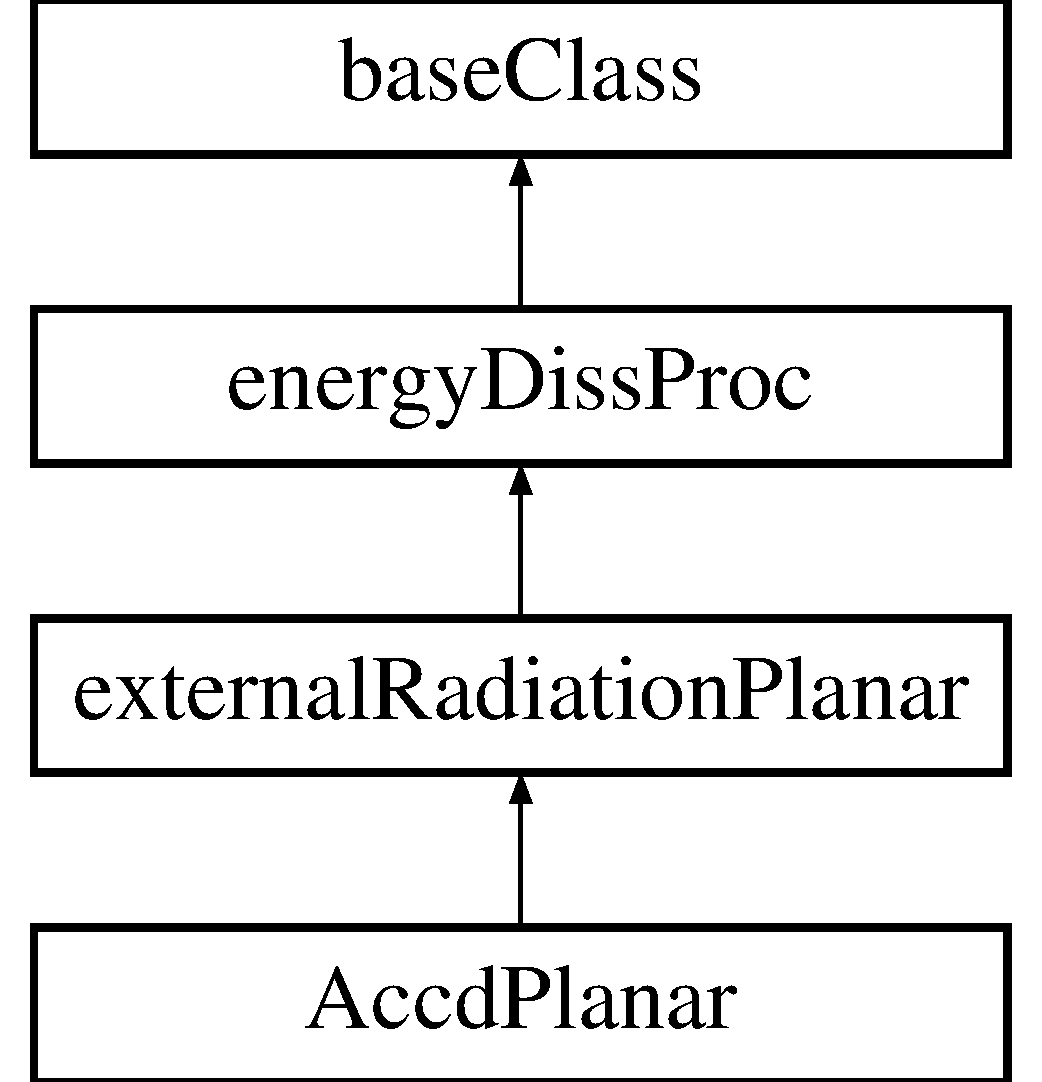
\includegraphics[height=4.000000cm]{classAccdPlanar}
\end{center}
\end{figure}


\subsection{Detailed Description}
Parameters used by class (defaults) 
\begin{DoxyParams}{Parameters}
{\em alpha} & (\hyperlink{classexternalRadiationPlanar}{external\-Radiation\-Planar}) ( alpha = -\/0.\-3333 ) \\
\hline
{\em R1} & -\/ (\hyperlink{classexternalRadiationPlanar}{external\-Radiation\-Planar}) accd lower boundary radius ('N\-E\-W' stratification) (R1 = 0.\-1$\ast$\-R\-\_\-sub) \\
\hline
{\em R2} & -\/ (\hyperlink{classexternalRadiationPlanar}{external\-Radiation\-Planar}) accd upper boundary radius ('N\-E\-W' stratification) (R2 = R\-\_\-sub) \\
\hline
{\em s} & -\/ (\hyperlink{classexternalRadiationPlanar}{external\-Radiation\-Planar}) stratification index ('N\-E\-W' stratification) (s = 2.\-0) \\
\hline
\end{DoxyParams}
\subsection*{Public Member Functions}
\begin{DoxyCompactItemize}
\item 
\hyperlink{classAccdPlanar_a380728055445c3f86558fa1fa8713871}{Accd\-Planar} (scfgp $\ast$\-\_\-cfg, \hyperlink{classjetGeometry}{jet\-Geometry} $\ast$\-\_\-r, \hyperlink{classelectrons}{electrons} $\ast$\-\_\-ele, std\-::string \-\_\-id)
\item 
\hyperlink{classAccdPlanar_a0e4ebd194cbee7b95a16cfe323ea645c}{$\sim$\-Accd\-Planar} ()
\item 
void \hyperlink{classAccdPlanar_a51960bc05d15aedf068b65a369d1899c}{print\-Info} ()
\item 
void \hyperlink{classAccdPlanar_a4e540b445accba0d2159f141ea682be3}{set\-Radius} ()
\item 
double \hyperlink{classAccdPlanar_a1f9a8eadf2626c50ecf0a56d5b9a17de}{getvext} (double \-\_\-\-R)
\item 
void \hyperlink{classAccdPlanar_ab4fdeb7f7898f380e2f9e333d430b2de}{setd\-Ld\-R} ()
\end{DoxyCompactItemize}
\subsection*{Additional Inherited Members}


\subsection{Constructor \& Destructor Documentation}
\hypertarget{classAccdPlanar_a380728055445c3f86558fa1fa8713871}{\index{Accd\-Planar@{Accd\-Planar}!Accd\-Planar@{Accd\-Planar}}
\index{Accd\-Planar@{Accd\-Planar}!AccdPlanar@{Accd\-Planar}}
\subsubsection[{Accd\-Planar}]{\setlength{\rightskip}{0pt plus 5cm}Accd\-Planar\-::\-Accd\-Planar (
\begin{DoxyParamCaption}
\item[{scfgp $\ast$}]{\-\_\-cfg, }
\item[{{\bf jet\-Geometry} $\ast$}]{\-\_\-r, }
\item[{{\bf electrons} $\ast$}]{\-\_\-ele, }
\item[{std\-::string}]{\-\_\-id}
\end{DoxyParamCaption}
)}}\label{classAccdPlanar_a380728055445c3f86558fa1fa8713871}
constructor 
\begin{DoxyParams}{Parameters}
{\em \-\_\-cfg} & -\/ scfgp class object \\
\hline
{\em \-\_\-r} & -\/ \hyperlink{classjetGeometry}{jet\-Geometry} class object \\
\hline
{\em \-\_\-ele} & -\/ electrons class object \\
\hline
{\em \-\_\-id} & \\
\hline
\end{DoxyParams}

\begin{DoxyCode}
9                                                                                  : 
      \hyperlink{classexternalRadiationPlanar_a6254e3256914a093886b7af1f1dc4876}{externalRadiationPlanar}( \hyperlink{classbaseClass_a744f87a6ebe63da08256c022d42a4ca7}{cfg}, \hyperlink{classbaseClass_a482bb9b1d94f3eb3f31026d14e9a2bb6}{r}, \hyperlink{classenergyDissProc_a0dbf0777938131e938c1fdad5df38a7f}{ele}, \textcolor{keywordtype}{id} ) \{
10   \textcolor{comment}{/* request parameters */}
11   \textcolor{comment}{/* -- */}
12 
13   \textcolor{keywordflow}{if}( R1 == 0.0 || R2 == 0.0 ) \{ \hyperlink{classAccdPlanar_a4e540b445accba0d2159f141ea682be3}{setRadius}( ); \}
14   \textcolor{keywordflow}{else} \{ bazinga::warning(\textcolor{keywordtype}{id},\textcolor{stringliteral}{"Overwritting R1 and R2 values from config file!"}); \}
15   
16   \hyperlink{classenergyDissProc_aafedd3c012010a8e8aa34247660fea3b}{vpMin} = 0.01*DSQR( \hyperlink{classenergyDissProc_a0dbf0777938131e938c1fdad5df38a7f}{ele} -> getGammaMin( ) )*\hyperlink{classAccdPlanar_a1f9a8eadf2626c50ecf0a56d5b9a17de}{getvext}( R2 );
17   vpMax = 100.0*DSQR( \hyperlink{classenergyDissProc_a0dbf0777938131e938c1fdad5df38a7f}{ele} -> getGammaMax( ) )*\hyperlink{classAccdPlanar_a1f9a8eadf2626c50ecf0a56d5b9a17de}{getvext}( R1 );
18 
19   \textcolor{comment}{/* initialize disk radius R;}
20 \textcolor{comment}{     here we use N-1 to use the same Upe as in other processes */}
21   R = \textcolor{keyword}{new} \hyperlink{classlogGeometry}{logGeometry}( R1, R2, \hyperlink{classbaseClass_a2b4d07d2b46197d495de0477f4bb22f8}{N}-1 );
22 
23   allocateUpe( ); \textcolor{comment}{// this is for storing matrix information about dUpe(r)/dR (R) }
24   allocateUpeR( ); \textcolor{comment}{// this is for storing vector information about Upe(r) }
25   allocateLpv( );
26   allocateLvPoint( );
27   allocateLvPointAvg( );
28 
29   \textcolor{keywordflow}{for}( \textcolor{keywordtype}{int} i=0;i<\hyperlink{classbaseClass_a2b4d07d2b46197d495de0477f4bb22f8}{N};i++ ) \{ set\_vp( i, \hyperlink{classenergyDissProc_aafedd3c012010a8e8aa34247660fea3b}{vpMin}*pow( vpMax/\hyperlink{classenergyDissProc_aafedd3c012010a8e8aa34247660fea3b}{vpMin},(\textcolor{keywordtype}{double})i/((\textcolor{keywordtype}{double})N-1)) ); \}
30 
31   \textcolor{comment}{/* set the values of dLdR */}
32   \hyperlink{classAccdPlanar_ab4fdeb7f7898f380e2f9e333d430b2de}{setdLdR}( ); \}
\end{DoxyCode}
\hypertarget{classAccdPlanar_a0e4ebd194cbee7b95a16cfe323ea645c}{\index{Accd\-Planar@{Accd\-Planar}!$\sim$\-Accd\-Planar@{$\sim$\-Accd\-Planar}}
\index{$\sim$\-Accd\-Planar@{$\sim$\-Accd\-Planar}!AccdPlanar@{Accd\-Planar}}
\subsubsection[{$\sim$\-Accd\-Planar}]{\setlength{\rightskip}{0pt plus 5cm}Accd\-Planar\-::$\sim$\-Accd\-Planar (
\begin{DoxyParamCaption}
{}
\end{DoxyParamCaption}
)}}\label{classAccdPlanar_a0e4ebd194cbee7b95a16cfe323ea645c}
destructor 
\begin{DoxyCode}
34                          \{
35   freeUpe( );
36   freeLpv( );
37   freeLvPoint( );
38   freeLvPointAvg( ); \}
\end{DoxyCode}


\subsection{Member Function Documentation}
\hypertarget{classAccdPlanar_a1f9a8eadf2626c50ecf0a56d5b9a17de}{\index{Accd\-Planar@{Accd\-Planar}!getvext@{getvext}}
\index{getvext@{getvext}!AccdPlanar@{Accd\-Planar}}
\subsubsection[{getvext}]{\setlength{\rightskip}{0pt plus 5cm}double Accd\-Planar\-::getvext (
\begin{DoxyParamCaption}
\item[{double}]{\-\_\-\-R}
\end{DoxyParamCaption}
)\hspace{0.3cm}{\ttfamily [virtual]}}}\label{classAccdPlanar_a1f9a8eadf2626c50ecf0a56d5b9a17de}
get v\-\_\-ext value in Hz 
\begin{DoxyParams}{Parameters}
{\em \-\_\-\-R} & -\/ radius in accretion disk plane \\
\hline
\end{DoxyParams}
\begin{DoxyReturn}{Returns}
v\-\_\-ext 
\end{DoxyReturn}


Reimplemented from \hyperlink{classexternalRadiationPlanar_aa9ea7f37d1e43219f71ec6b215a38b96}{external\-Radiation\-Planar}.


\begin{DoxyCode}
77                                       \{
78   \textcolor{keywordtype}{double} Ledd = 1.3e47*mBH;
79   \textcolor{keywordtype}{double} Ldisk = eDisk*mDot*Ledd;
80   \textcolor{keywordtype}{double} vext = 0.0;
81   \textcolor{keywordtype}{double} Fdisk;
82   \textcolor{keywordflow}{if}( \hyperlink{classenergyDissProc_a0a23854c1c830dfb9ac33d116fce5b7d}{luminosityConstNu} ) \{ Fdisk = (3.0*G\_CONST*mBH*1e09*MSUN)*mDot*Ledd/( DSQR(
      LIGHT\_SPEED)*8.0*M\_PI*pow(R2,3.0) ); \}
83   \textcolor{keywordflow}{else} \{ Fdisk = (3.0*G\_CONST*mBH*1e09*MSUN)*mDot*Ledd/( DSQR(LIGHT\_SPEED)*8.0*M\_PI*pow(\_R,3.0) ); \}
84   \textcolor{keywordtype}{double} Teff = pow( Fdisk/SIGMA\_SB, 0.25 );
85   vext = 3.92*Teff*K\_BOLTZMAN/PLANCK\_H;
86   \textcolor{keywordflow}{return} vext; \}
\end{DoxyCode}
\hypertarget{classAccdPlanar_a51960bc05d15aedf068b65a369d1899c}{\index{Accd\-Planar@{Accd\-Planar}!print\-Info@{print\-Info}}
\index{print\-Info@{print\-Info}!AccdPlanar@{Accd\-Planar}}
\subsubsection[{print\-Info}]{\setlength{\rightskip}{0pt plus 5cm}void Accd\-Planar\-::print\-Info (
\begin{DoxyParamCaption}
{}
\end{DoxyParamCaption}
)\hspace{0.3cm}{\ttfamily [virtual]}}}\label{classAccdPlanar_a51960bc05d15aedf068b65a369d1899c}
print basic information about myself (virtual) 

Reimplemented from \hyperlink{classexternalRadiationPlanar_a47e497b12dfa4e71311bffb3a4b384b2}{external\-Radiation\-Planar}.


\begin{DoxyCode}
40                             \{
41   bazinga::info(\textcolor{keywordtype}{id},\textcolor{stringliteral}{"Info"});
42   bazinga::print\_info(\textcolor{keywordtype}{id},\textcolor{stringliteral}{"N"},\hyperlink{classbaseClass_a2b4d07d2b46197d495de0477f4bb22f8}{N});
43   bazinga::info(\textcolor{keywordtype}{id},\textcolor{stringliteral}{"Using stratification version NEW (only option)"});
44   bazinga::print\_info(\textcolor{keywordtype}{id},\textcolor{stringliteral}{"radius R1"},R1,\textcolor{stringliteral}{"cm"});
45   bazinga::print\_info(\textcolor{keywordtype}{id},\textcolor{stringliteral}{"radius R2"},R2,\textcolor{stringliteral}{"cm"});
46   bazinga::print\_info(\textcolor{keywordtype}{id},\textcolor{stringliteral}{"stratification index"},s);
47   bazinga::print\_info(\textcolor{keywordtype}{id},\textcolor{stringliteral}{"alpha"},alpha);
48   bazinga::print\_info(\textcolor{keywordtype}{id},\textcolor{stringliteral}{"vpMin"},\hyperlink{classenergyDissProc_aafedd3c012010a8e8aa34247660fea3b}{vpMin},\textcolor{stringliteral}{"Hz"});
49   bazinga::print\_info(\textcolor{keywordtype}{id},\textcolor{stringliteral}{"vpMax"},vpMax,\textcolor{stringliteral}{"Hz"});
50   \textcolor{keywordflow}{if}( approx ) \{ bazinga::info(\textcolor{keywordtype}{id},\textcolor{stringliteral}{"Using approximate dependence on R"}); \} 
51   \textcolor{keywordflow}{if}( \hyperlink{classenergyDissProc_a2cc4e4eae15982f977a0dfa5458d80f4}{luminosityConstU} ) \{ bazinga::warning(\textcolor{keywordtype}{id},\textcolor{stringliteral}{"Using constant u' to calculate luminosity."}
      ); \}
52   \textcolor{keywordflow}{if}( \hyperlink{classenergyDissProc_a0a23854c1c830dfb9ac33d116fce5b7d}{luminosityConstNu} ) \{ bazinga::warning(\textcolor{keywordtype}{id},\textcolor{stringliteral}{"Using constant v\_ext to calculate
       luminosity."}); \}
53 \}
\end{DoxyCode}
\hypertarget{classAccdPlanar_ab4fdeb7f7898f380e2f9e333d430b2de}{\index{Accd\-Planar@{Accd\-Planar}!setd\-Ld\-R@{setd\-Ld\-R}}
\index{setd\-Ld\-R@{setd\-Ld\-R}!AccdPlanar@{Accd\-Planar}}
\subsubsection[{setd\-Ld\-R}]{\setlength{\rightskip}{0pt plus 5cm}void Accd\-Planar\-::setd\-Ld\-R (
\begin{DoxyParamCaption}
{}
\end{DoxyParamCaption}
)\hspace{0.3cm}{\ttfamily [virtual]}}}\label{classAccdPlanar_ab4fdeb7f7898f380e2f9e333d430b2de}
set d\-L/d\-R for particulat source 

Reimplemented from \hyperlink{classexternalRadiationPlanar_a7914df2de2d822755ac1c9e6d860e22b}{external\-Radiation\-Planar}.


\begin{DoxyCode}
63                           \{
64   \textcolor{keywordtype}{double} Ledd = 1.3e47*mBH;
65   \textcolor{keywordtype}{double} Ldisk = eDisk*mDot*Ledd;
66   \textcolor{comment}{/* fill in dLdR vector that will be used for the rest of the calculations */}
67   bazinga::info(\textcolor{keywordtype}{id},\textcolor{stringliteral}{"Seeting dLdR."});
68   \textcolor{keywordflow}{for}( \textcolor{keywordtype}{int} i=0;i<R->getMaxIndex();i++ ) \{
69       R->update( i );
70       \textcolor{keywordtype}{double} val = 0.0;
71       val = (3.0*G\_CONST*mBH*1e09*MSUN)*mDot*Ledd*pow(R->get(),-s)/( 2.0*DSQR(LIGHT\_SPEED) );
72       gsl\_vector\_set( dLdR, R->getIndex( ), val ); \}
73   \textcolor{comment}{/* Now when we have all set let us save what we have just calculated - dLdR */}
74   bazinga::info(\textcolor{keywordtype}{id},\textcolor{stringliteral}{"Saving dLdR."});
75   bazinga::save\_GSLVector( \textcolor{stringliteral}{"dLdR\_"}+this->\hyperlink{classbaseClass_a756d5accf10ced9a34024048c95a51c9}{whoAmI}( ), R->getRadius\_GSLVector( ), dLdR, 
      \hyperlink{classbaseClass_a744f87a6ebe63da08256c022d42a4ca7}{cfg}->get<std::string>(\textcolor{stringliteral}{"output"}) ); \}
\end{DoxyCode}
\hypertarget{classAccdPlanar_a4e540b445accba0d2159f141ea682be3}{\index{Accd\-Planar@{Accd\-Planar}!set\-Radius@{set\-Radius}}
\index{set\-Radius@{set\-Radius}!AccdPlanar@{Accd\-Planar}}
\subsubsection[{set\-Radius}]{\setlength{\rightskip}{0pt plus 5cm}void Accd\-Planar\-::set\-Radius (
\begin{DoxyParamCaption}
{}
\end{DoxyParamCaption}
)\hspace{0.3cm}{\ttfamily [virtual]}}}\label{classAccdPlanar_a4e540b445accba0d2159f141ea682be3}
sets rext if not provided by config file 

Reimplemented from \hyperlink{classexternalRadiationPlanar_a710859cda6258d75098ccb31e60ab261}{external\-Radiation\-Planar}.


\begin{DoxyCode}
55                             \{
56   \textcolor{keywordtype}{double} Ledd = 1.3e47*mBH;
57   \textcolor{keywordtype}{double} Ldisk = eDisk*mDot*Ledd;
58   \textcolor{keywordtype}{double} R\_sub = 1.6e-5*sqrt( Ldisk );
59   \textcolor{keywordtype}{double} Rg = mBH*1e09*MSUN*G\_CONST/DSQR(LIGHT\_SPEED);
60   R1 = Rg/(2.0*eDisk);
61   R2 = R\_sub; \}
\end{DoxyCode}


The documentation for this class was generated from the following files\-:\begin{DoxyCompactItemize}
\item 
/home/mjaniak/\-Soft/blazar++/include/\hyperlink{AccdPlanar_8hpp}{Accd\-Planar.\-hpp}\item 
/home/mjaniak/\-Soft/blazar++/src/\hyperlink{AccdPlanar_8cpp}{Accd\-Planar.\-cpp}\end{DoxyCompactItemize}

\hypertarget{classAccdSphericalGu}{\section{Accd\-Spherical\-Gu Class Reference}
\label{classAccdSphericalGu}\index{Accd\-Spherical\-Gu@{Accd\-Spherical\-Gu}}
}


{\ttfamily \#include $<$Accd\-Spherical\-Gu.\-hpp$>$}

Inheritance diagram for Accd\-Spherical\-Gu\-:\begin{figure}[H]
\begin{center}
\leavevmode
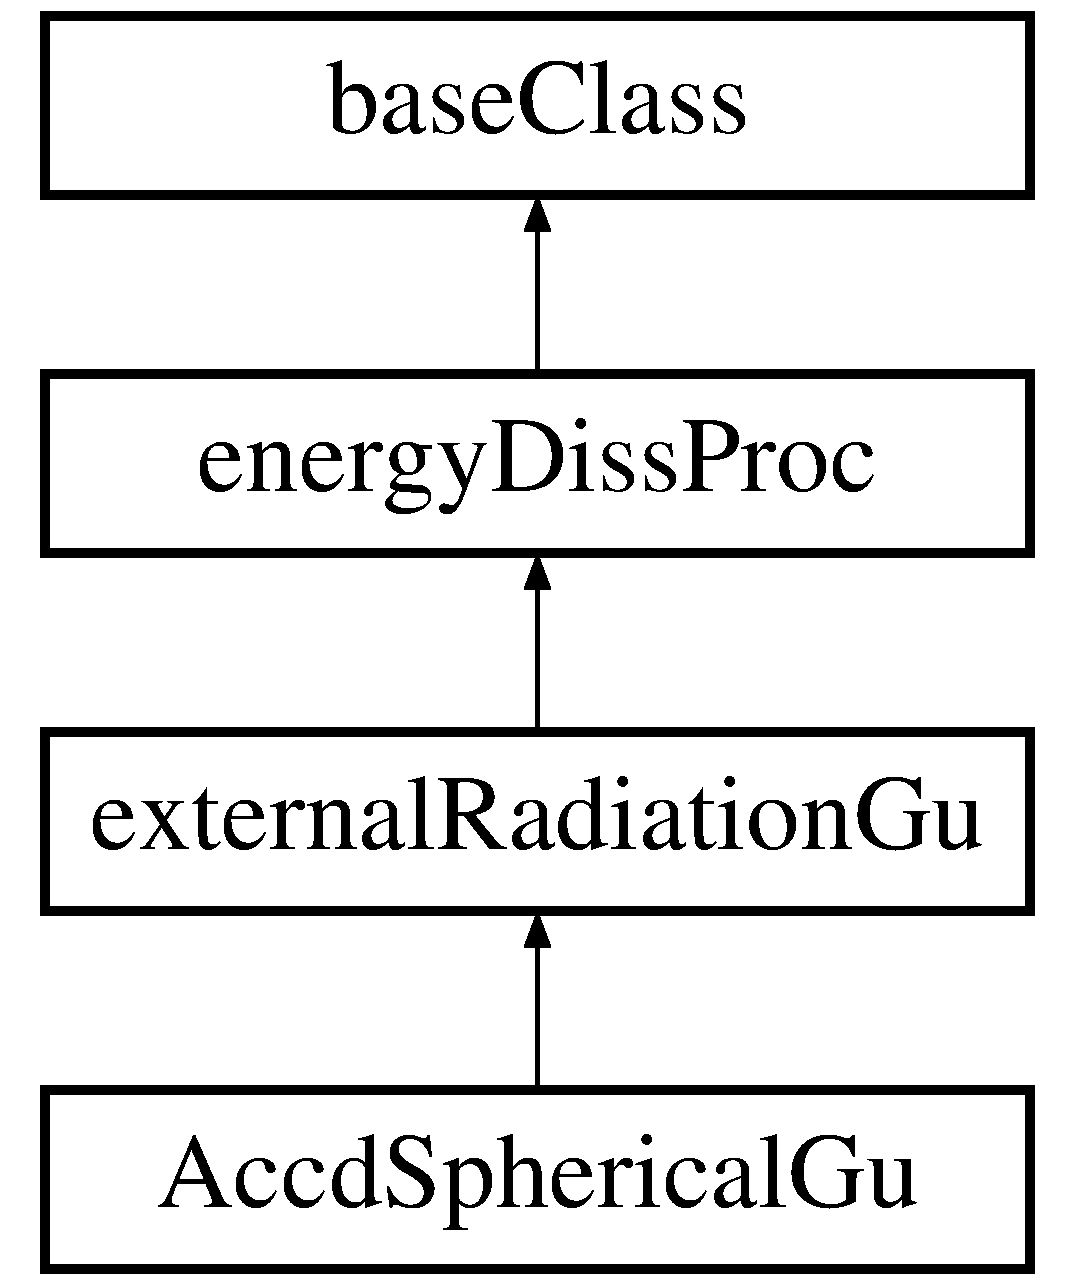
\includegraphics[height=4.000000cm]{classAccdSphericalGu}
\end{center}
\end{figure}


\subsection{Detailed Description}
Parameters used by class (defaults) 
\begin{DoxyParams}{Parameters}
{\em rext} & -\/ accretion disk inner radius \\
\hline
\end{DoxyParams}
\subsection*{Public Member Functions}
\begin{DoxyCompactItemize}
\item 
\hyperlink{classAccdSphericalGu_a0ce695a3b46e6027bb770e6b9c2ac2ae}{Accd\-Spherical\-Gu} (scfgp $\ast$\-\_\-cfg, \hyperlink{classjetGeometry}{jet\-Geometry} $\ast$\-\_\-r, \hyperlink{classelectrons}{electrons} $\ast$\-\_\-ele, std\-::string \-\_\-id)
\item 
\hyperlink{classAccdSphericalGu_ad5dfde0d63207ba0c2a14d6e8f9561e4}{$\sim$\-Accd\-Spherical\-Gu} ()
\item 
void \hyperlink{classAccdSphericalGu_a672f673606422556c3fb31a1787c6724}{print\-Info} ()
\item 
void \hyperlink{classAccdSphericalGu_a278cae9b07c99dd7398121a77fa069c9}{update} ()
\item 
double \hyperlink{classAccdSphericalGu_a802ac0782b844446953d4b59da160e46}{getvext} (double \-\_\-r)
\item 
void \hyperlink{classAccdSphericalGu_a606c270f0d33338544b48373fe294f6b}{set\-Radius} ()
\end{DoxyCompactItemize}
\subsection*{Additional Inherited Members}


\subsection{Constructor \& Destructor Documentation}
\hypertarget{classAccdSphericalGu_a0ce695a3b46e6027bb770e6b9c2ac2ae}{\index{Accd\-Spherical\-Gu@{Accd\-Spherical\-Gu}!Accd\-Spherical\-Gu@{Accd\-Spherical\-Gu}}
\index{Accd\-Spherical\-Gu@{Accd\-Spherical\-Gu}!AccdSphericalGu@{Accd\-Spherical\-Gu}}
\subsubsection[{Accd\-Spherical\-Gu}]{\setlength{\rightskip}{0pt plus 5cm}Accd\-Spherical\-Gu\-::\-Accd\-Spherical\-Gu (
\begin{DoxyParamCaption}
\item[{scfgp $\ast$}]{\-\_\-cfg, }
\item[{{\bf jet\-Geometry} $\ast$}]{\-\_\-r, }
\item[{{\bf electrons} $\ast$}]{\-\_\-ele, }
\item[{std\-::string}]{\-\_\-id}
\end{DoxyParamCaption}
)}}\label{classAccdSphericalGu_a0ce695a3b46e6027bb770e6b9c2ac2ae}
constructor 
\begin{DoxyParams}{Parameters}
{\em \-\_\-cfg} & -\/ scfgp class object \\
\hline
{\em \-\_\-r} & -\/ \hyperlink{classjetGeometry}{jet\-Geometry} class object \\
\hline
{\em \-\_\-ele} & -\/ electrons class object \\
\hline
{\em \-\_\-id} & \\
\hline
\end{DoxyParams}

\begin{DoxyCode}
9                                                                                            : 
      \hyperlink{classexternalRadiationGu_aad5903b642f08594be10d699cf9fb3b4}{externalRadiationGu}( \hyperlink{classbaseClass_a744f87a6ebe63da08256c022d42a4ca7}{cfg}, \hyperlink{classbaseClass_a482bb9b1d94f3eb3f31026d14e9a2bb6}{r}, \hyperlink{classenergyDissProc_a0dbf0777938131e938c1fdad5df38a7f}{ele}, \textcolor{keywordtype}{id} ) \{
10   \textcolor{comment}{/* requested parameters */}
11 \textcolor{comment}{//  cfg -> request<double>(id + "e", 10.0, &e );}
12 \textcolor{comment}{//  cfg -> request<double>(id + "cf", 0.1, &cf );}
13   \hyperlink{classbaseClass_a744f87a6ebe63da08256c022d42a4ca7}{cfg} -> request<double>(\textcolor{keywordtype}{id} + \textcolor{stringliteral}{"rext"}, 0.0, &rext );
14 \textcolor{comment}{//  cfg -> request<double>(id + "k", 3.0, &k );}
15 \textcolor{comment}{//}
16   \hyperlink{classbaseClass_a744f87a6ebe63da08256c022d42a4ca7}{cfg} -> updateRequests( );
17 
18   \textcolor{keywordflow}{if}( rext == 0.0 ) \{ \hyperlink{classAccdSphericalGu_a606c270f0d33338544b48373fe294f6b}{setRadius}( ); \}
19   \textcolor{keywordflow}{else} \{ bazinga::warning(\textcolor{keywordtype}{id},\textcolor{stringliteral}{"Overwritting rext value from config file!"}); \}
20   
21   \hyperlink{classenergyDissProc_aafedd3c012010a8e8aa34247660fea3b}{vpMin} = 0.01*DSQR( \hyperlink{classenergyDissProc_a0dbf0777938131e938c1fdad5df38a7f}{ele} -> getGammaMin( ) )*\hyperlink{classAccdSphericalGu_a802ac0782b844446953d4b59da160e46}{getvext}( \hyperlink{classbaseClass_a482bb9b1d94f3eb3f31026d14e9a2bb6}{r}->getRMax() );
22   vpMax = 100.0*DSQR( \hyperlink{classenergyDissProc_a0dbf0777938131e938c1fdad5df38a7f}{ele} -> getGammaMax( ) )*\hyperlink{classAccdSphericalGu_a802ac0782b844446953d4b59da160e46}{getvext}( \hyperlink{classbaseClass_a482bb9b1d94f3eb3f31026d14e9a2bb6}{r}->getR0() );
23 
24   allocateUpeR( ); \textcolor{comment}{// this is for storing vector information about Upe(r) }
25   allocateLpv( );
26   allocateLvPoint( );
27   allocateLvPointAvg( );
28 
29   \textcolor{keywordflow}{for}( \textcolor{keywordtype}{int} i=0;i<\hyperlink{classbaseClass_a2b4d07d2b46197d495de0477f4bb22f8}{N};i++ ) \{ set\_vp( i, \hyperlink{classenergyDissProc_aafedd3c012010a8e8aa34247660fea3b}{vpMin}*pow( vpMax/\hyperlink{classenergyDissProc_aafedd3c012010a8e8aa34247660fea3b}{vpMin},(\textcolor{keywordtype}{double})i/((\textcolor{keywordtype}{double})N-1)) ); \}
30 \}
\end{DoxyCode}
\hypertarget{classAccdSphericalGu_ad5dfde0d63207ba0c2a14d6e8f9561e4}{\index{Accd\-Spherical\-Gu@{Accd\-Spherical\-Gu}!$\sim$\-Accd\-Spherical\-Gu@{$\sim$\-Accd\-Spherical\-Gu}}
\index{$\sim$\-Accd\-Spherical\-Gu@{$\sim$\-Accd\-Spherical\-Gu}!AccdSphericalGu@{Accd\-Spherical\-Gu}}
\subsubsection[{$\sim$\-Accd\-Spherical\-Gu}]{\setlength{\rightskip}{0pt plus 5cm}Accd\-Spherical\-Gu\-::$\sim$\-Accd\-Spherical\-Gu (
\begin{DoxyParamCaption}
{}
\end{DoxyParamCaption}
)\hspace{0.3cm}{\ttfamily [inline]}}}\label{classAccdSphericalGu_ad5dfde0d63207ba0c2a14d6e8f9561e4}
destructor 
\begin{DoxyCode}
33 \{ \}
\end{DoxyCode}


\subsection{Member Function Documentation}
\hypertarget{classAccdSphericalGu_a802ac0782b844446953d4b59da160e46}{\index{Accd\-Spherical\-Gu@{Accd\-Spherical\-Gu}!getvext@{getvext}}
\index{getvext@{getvext}!AccdSphericalGu@{Accd\-Spherical\-Gu}}
\subsubsection[{getvext}]{\setlength{\rightskip}{0pt plus 5cm}double Accd\-Spherical\-Gu\-::getvext (
\begin{DoxyParamCaption}
\item[{double}]{\-\_\-r}
\end{DoxyParamCaption}
)\hspace{0.3cm}{\ttfamily [virtual]}}}\label{classAccdSphericalGu_a802ac0782b844446953d4b59da160e46}
get v\-\_\-ext value in Hz 
\begin{DoxyParams}{Parameters}
{\em \-\_\-r} & -\/ radius \\
\hline
\end{DoxyParams}
\begin{DoxyReturn}{Returns}
v\-\_\-ext 
\end{DoxyReturn}


Reimplemented from \hyperlink{classexternalRadiationGu_ab7e1abcc40cf0538404e88a0febdfb02}{external\-Radiation\-Gu}.


\begin{DoxyCode}
32                                            \{
33   \textcolor{keywordtype}{double} Ledd = 1.3e47*mBH;
34   \textcolor{keywordtype}{double} Ldisk = eDisk*mDot*Ledd;
35   \textcolor{keywordtype}{double} vext = 0.0;
36   \textcolor{keywordtype}{double} Fdisk;
37   \textcolor{keywordflow}{if}( \hyperlink{classenergyDissProc_a0a23854c1c830dfb9ac33d116fce5b7d}{luminosityConstNu} ) \{ Fdisk = (3.0*G\_CONST*mBH*1e09*MSUN)*mDot*Ledd/( DSQR(
      LIGHT\_SPEED)*8.0*M\_PI*pow(\_r,3.0) ); \}
38   \textcolor{keywordflow}{else} \{ Fdisk = (3.0*G\_CONST*mBH*1e09*MSUN)*mDot*Ledd/( DSQR(LIGHT\_SPEED)*8.0*M\_PI*pow(\_r,3.0) ); \}
39   \textcolor{keywordtype}{double} Teff = pow( Fdisk/SIGMA\_SB, 0.25 );
40   vext = 3.92*Teff*K\_BOLTZMAN/PLANCK\_H;
41   \textcolor{keywordflow}{return} vext; \}
\end{DoxyCode}
\hypertarget{classAccdSphericalGu_a672f673606422556c3fb31a1787c6724}{\index{Accd\-Spherical\-Gu@{Accd\-Spherical\-Gu}!print\-Info@{print\-Info}}
\index{print\-Info@{print\-Info}!AccdSphericalGu@{Accd\-Spherical\-Gu}}
\subsubsection[{print\-Info}]{\setlength{\rightskip}{0pt plus 5cm}void Accd\-Spherical\-Gu\-::print\-Info (
\begin{DoxyParamCaption}
{}
\end{DoxyParamCaption}
)\hspace{0.3cm}{\ttfamily [virtual]}}}\label{classAccdSphericalGu_a672f673606422556c3fb31a1787c6724}
print basic information about myself (virtual) 

Reimplemented from \hyperlink{classexternalRadiationGu_a8aa28d939b0ecf2651f18cc4f5f6ba25}{external\-Radiation\-Gu}.


\begin{DoxyCode}
55                                  \{
56   bazinga::info(\textcolor{keywordtype}{id},\textcolor{stringliteral}{"Info"});
57   bazinga::print\_info(\textcolor{keywordtype}{id},\textcolor{stringliteral}{"N"},\hyperlink{classbaseClass_a2b4d07d2b46197d495de0477f4bb22f8}{N});
58   bazinga::print\_info(\textcolor{keywordtype}{id},\textcolor{stringliteral}{"Avg energy (in external frame)"},\hyperlink{classAccdSphericalGu_a802ac0782b844446953d4b59da160e46}{getvext}( \hyperlink{classbaseClass_a482bb9b1d94f3eb3f31026d14e9a2bb6}{r}->getR0())*PLANCK\_H,\textcolor{stringliteral}{"eV"});
59   bazinga::print\_info(\textcolor{keywordtype}{id},\textcolor{stringliteral}{"Avg frequency (in external frame)"},\hyperlink{classAccdSphericalGu_a802ac0782b844446953d4b59da160e46}{getvext}( \hyperlink{classbaseClass_a482bb9b1d94f3eb3f31026d14e9a2bb6}{r}->getR0()),\textcolor{stringliteral}{"Hz"});
60   bazinga::print\_info(\textcolor{keywordtype}{id},\textcolor{stringliteral}{"radius rext"},rext,\textcolor{stringliteral}{"cm"});
61   bazinga::print\_info(\textcolor{keywordtype}{id},\textcolor{stringliteral}{"vpMin"},\hyperlink{classenergyDissProc_aafedd3c012010a8e8aa34247660fea3b}{vpMin},\textcolor{stringliteral}{"Hz"});
62   bazinga::print\_info(\textcolor{keywordtype}{id},\textcolor{stringliteral}{"vpMax"},vpMax,\textcolor{stringliteral}{"Hz"});
63 \}
\end{DoxyCode}
\hypertarget{classAccdSphericalGu_a606c270f0d33338544b48373fe294f6b}{\index{Accd\-Spherical\-Gu@{Accd\-Spherical\-Gu}!set\-Radius@{set\-Radius}}
\index{set\-Radius@{set\-Radius}!AccdSphericalGu@{Accd\-Spherical\-Gu}}
\subsubsection[{set\-Radius}]{\setlength{\rightskip}{0pt plus 5cm}void Accd\-Spherical\-Gu\-::set\-Radius (
\begin{DoxyParamCaption}
{}
\end{DoxyParamCaption}
)\hspace{0.3cm}{\ttfamily [virtual]}}}\label{classAccdSphericalGu_a606c270f0d33338544b48373fe294f6b}
sets rext if not provided by config file 

Reimplemented from \hyperlink{classexternalRadiationGu_a541b2bb7da733f10d83af6225b7ad5f8}{external\-Radiation\-Gu}.


\begin{DoxyCode}
65                                   \{
66   \textcolor{keywordtype}{double} Ledd = 1.3e47*mBH;
67   \textcolor{keywordtype}{double} Ldisk = eDisk*mDot*Ledd;
68   \textcolor{keywordtype}{double} R\_sub = 1.6e-5*sqrt( Ldisk );
69   \textcolor{keywordtype}{double} Rg = mBH*1e09*MSUN*G\_CONST/DSQR(LIGHT\_SPEED);
70   rext = Rg; \}
\end{DoxyCode}
\hypertarget{classAccdSphericalGu_a278cae9b07c99dd7398121a77fa069c9}{\index{Accd\-Spherical\-Gu@{Accd\-Spherical\-Gu}!update@{update}}
\index{update@{update}!AccdSphericalGu@{Accd\-Spherical\-Gu}}
\subsubsection[{update}]{\setlength{\rightskip}{0pt plus 5cm}void Accd\-Spherical\-Gu\-::update (
\begin{DoxyParamCaption}
{}
\end{DoxyParamCaption}
)\hspace{0.3cm}{\ttfamily [virtual]}}}\label{classAccdSphericalGu_a278cae9b07c99dd7398121a77fa069c9}
calculate and set Upe every time with new radius r 

Reimplemented from \hyperlink{classexternalRadiationGu_a730363f393f29aef9927e0bb84087116}{external\-Radiation\-Gu}.


\begin{DoxyCode}
43                                \{
44   \textcolor{keywordtype}{double} Ledd = 1.3e47*mBH;
45   \textcolor{keywordtype}{double} Ldisk = eDisk*mDot*Ledd;
46   \textcolor{keywordtype}{double} temp\_upe = 0.0;
47   \textcolor{keywordtype}{double} temp\_cf = 0.0;
48   temp\_cf = 0.75*(((0.28*rext)/\hyperlink{classbaseClass_a482bb9b1d94f3eb3f31026d14e9a2bb6}{r}->get())+(1.0/(4.0*DSQR(Gamma)*DSQR(Gamma))));
49   temp\_upe = (temp\_cf*Ldisk*DSQR(Gamma))/(3.0*M\_PI*DSQR(\hyperlink{classbaseClass_a482bb9b1d94f3eb3f31026d14e9a2bb6}{r}->get())*LIGHT\_SPEED);
50   gsl\_vector\_set( \hyperlink{classenergyDissProc_ac925d66519c79f36421f75a6bc9f0965}{upe\_r}, \hyperlink{classbaseClass_a482bb9b1d94f3eb3f31026d14e9a2bb6}{r}->getIndex( ), temp\_upe );
51   bazinga::print\_info(\textcolor{keywordtype}{id},\textcolor{stringliteral}{"Upe"},gsl\_vector\_get( \hyperlink{classenergyDissProc_ac925d66519c79f36421f75a6bc9f0965}{upe\_r}, \hyperlink{classbaseClass_a482bb9b1d94f3eb3f31026d14e9a2bb6}{r}->getIndex( ) ) );
52   set\_upe\_r( gsl\_vector\_get( \hyperlink{classenergyDissProc_ac925d66519c79f36421f75a6bc9f0965}{upe\_r}, \hyperlink{classbaseClass_a482bb9b1d94f3eb3f31026d14e9a2bb6}{r}->getIndex( ) ) );
53   \hyperlink{classenergyDissProc_a7b51925f603e271657cab66afe822591}{flag\_upe\_r} = \textcolor{keyword}{false}; \}
\end{DoxyCode}


The documentation for this class was generated from the following files\-:\begin{DoxyCompactItemize}
\item 
/home/mjaniak/\-Soft/blazar++/include/\hyperlink{AccdSphericalGu_8hpp}{Accd\-Spherical\-Gu.\-hpp}\item 
/home/mjaniak/\-Soft/blazar++/src/Accd\-Spherical\-Gu.\-cpp\end{DoxyCompactItemize}

\hypertarget{classbaseClass}{\section{base\-Class Class Reference}
\label{classbaseClass}\index{base\-Class@{base\-Class}}
}


{\ttfamily \#include $<$base\-Class.\-hpp$>$}

Inheritance diagram for base\-Class\-:\begin{figure}[H]
\begin{center}
\leavevmode
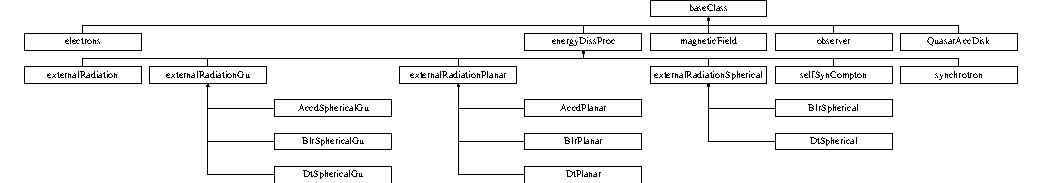
\includegraphics[height=2.456140cm]{classbaseClass}
\end{center}
\end{figure}


\subsection{Detailed Description}
Base class for all other classes used in blazar++. Provides unified way of sharing scfgp, id and \hyperlink{classjetGeometry}{jet\-Geometry} \subsection*{Public Member Functions}
\begin{DoxyCompactItemize}
\item 
\hypertarget{classbaseClass_a5771803aa5b82f52a1dcb6679fc047be}{{\bfseries base\-Class} (scfgp $\ast$\hyperlink{classbaseClass_a744f87a6ebe63da08256c022d42a4ca7}{cfg}, \hyperlink{classjetGeometry}{jet\-Geometry} $\ast$\hyperlink{classbaseClass_a482bb9b1d94f3eb3f31026d14e9a2bb6}{r}, std\-::string \hyperlink{classbaseClass_a4d5ff386a69bcbe21b5976f55b624df6}{id})}\label{classbaseClass_a5771803aa5b82f52a1dcb6679fc047be}

\item 
std\-::string \hyperlink{classbaseClass_a756d5accf10ced9a34024048c95a51c9}{who\-Am\-I} ()
\item 
virtual void \hyperlink{classbaseClass_a67f911cca483b620b908c69dfa4f3ad7}{print\-Info} ()
\item 
double \hyperlink{classbaseClass_a208facecf3a4480b47bebfce91413a39}{beta} (double x)
\item 
int \hyperlink{classbaseClass_a6ba5c4ce24742db73f45064337cf6963}{get\-N} ()
\end{DoxyCompactItemize}
\subsection*{Public Attributes}
\begin{DoxyCompactItemize}
\item 
std\-::string \hyperlink{classbaseClass_a4d5ff386a69bcbe21b5976f55b624df6}{id}
\item 
scfgp $\ast$ \hyperlink{classbaseClass_a744f87a6ebe63da08256c022d42a4ca7}{cfg}
\item 
\hyperlink{classjetGeometry}{jet\-Geometry} $\ast$ \hyperlink{classbaseClass_a482bb9b1d94f3eb3f31026d14e9a2bb6}{r}
\item 
int \hyperlink{classbaseClass_a2b4d07d2b46197d495de0477f4bb22f8}{N}
\end{DoxyCompactItemize}


\subsection{Member Function Documentation}
\hypertarget{classbaseClass_a208facecf3a4480b47bebfce91413a39}{\index{base\-Class@{base\-Class}!beta@{beta}}
\index{beta@{beta}!baseClass@{base\-Class}}
\subsubsection[{beta}]{\setlength{\rightskip}{0pt plus 5cm}double base\-Class\-::beta (
\begin{DoxyParamCaption}
\item[{double}]{x}
\end{DoxyParamCaption}
)}}\label{classbaseClass_a208facecf3a4480b47bebfce91413a39}
get beta from Lorentz factor ; it shouldn't probably be here 
\begin{DoxyCode}
16 \{ \textcolor{keywordflow}{return} sqrt(1.0-1.0/(x*x)); \}
\end{DoxyCode}
\hypertarget{classbaseClass_a6ba5c4ce24742db73f45064337cf6963}{\index{base\-Class@{base\-Class}!get\-N@{get\-N}}
\index{get\-N@{get\-N}!baseClass@{base\-Class}}
\subsubsection[{get\-N}]{\setlength{\rightskip}{0pt plus 5cm}int base\-Class\-::get\-N (
\begin{DoxyParamCaption}
{}
\end{DoxyParamCaption}
)\hspace{0.3cm}{\ttfamily [inline]}}}\label{classbaseClass_a6ba5c4ce24742db73f45064337cf6963}
get N 
\begin{DoxyCode}
51 \{ \textcolor{keywordflow}{return} \hyperlink{classbaseClass_a2b4d07d2b46197d495de0477f4bb22f8}{N}; \}
\end{DoxyCode}
\hypertarget{classbaseClass_a67f911cca483b620b908c69dfa4f3ad7}{\index{base\-Class@{base\-Class}!print\-Info@{print\-Info}}
\index{print\-Info@{print\-Info}!baseClass@{base\-Class}}
\subsubsection[{print\-Info}]{\setlength{\rightskip}{0pt plus 5cm}virtual void base\-Class\-::print\-Info (
\begin{DoxyParamCaption}
{}
\end{DoxyParamCaption}
)\hspace{0.3cm}{\ttfamily [inline]}, {\ttfamily [virtual]}}}\label{classbaseClass_a67f911cca483b620b908c69dfa4f3ad7}
print basic information about myself (virtual) 

Reimplemented in \hyperlink{classelectrons_ace657f207a4f68058b2606ff2772f3c5}{electrons}, \hyperlink{classenergyDissProc_ad1fbde0f7635a19a81412b9766916eb9}{energy\-Diss\-Proc}, \hyperlink{classobserver_a1fbeb6a33647dfadbb1ca9c0d64953bb}{observer}, \hyperlink{classexternalRadiationPlanar_a47e497b12dfa4e71311bffb3a4b384b2}{external\-Radiation\-Planar}, \hyperlink{classmagneticField_a9a0793b3b3a94962aaea1052edfe9b28}{magnetic\-Field}, \hyperlink{classQuasarAccDisk_aab9e9fbad17ba40931219473918896a7}{Quasar\-Acc\-Disk}, \hyperlink{classDtSpherical_a14440ec30b997fe2461c07f4507dd994}{Dt\-Spherical}, \hyperlink{classBlrPlanar_a3321d83625869e16c5794d9419dff073}{Blr\-Planar}, \hyperlink{classsynchrotron_a6a8610b523a6e3c656372537ad28b756}{synchrotron}, \hyperlink{classBlrSpherical_a101b95271855f15f1049fcea9efde235}{Blr\-Spherical}, \hyperlink{classexternalRadiationSpherical_a232684df0d246d8c5ec06e832bbaad0f}{external\-Radiation\-Spherical}, \hyperlink{classDtPlanar_a0d1b6697d54a08030ed50b7e4b5fbfef}{Dt\-Planar}, \hyperlink{classselfSynCompton_a46f692985a0fd74c14a018cc43f25c0b}{self\-Syn\-Compton}, \hyperlink{classAccdPlanar_a51960bc05d15aedf068b65a369d1899c}{Accd\-Planar}, \hyperlink{classexternalRadiationGu_a8aa28d939b0ecf2651f18cc4f5f6ba25}{external\-Radiation\-Gu}, \hyperlink{classBlrSphericalGu_a69de552417b7b01c3634650aaa9413d7}{Blr\-Spherical\-Gu}, \hyperlink{classDtSphericalGu_aeed0bda6440570b686aaf85bf5d2b6b3}{Dt\-Spherical\-Gu}, \hyperlink{classAccdSphericalGu_a672f673606422556c3fb31a1787c6724}{Accd\-Spherical\-Gu}, and \hyperlink{classexternalRadiation_a8747348f3468165fca0c5547e207b5a9}{external\-Radiation}.


\begin{DoxyCode}
45 \{ \};
\end{DoxyCode}
\hypertarget{classbaseClass_a756d5accf10ced9a34024048c95a51c9}{\index{base\-Class@{base\-Class}!who\-Am\-I@{who\-Am\-I}}
\index{who\-Am\-I@{who\-Am\-I}!baseClass@{base\-Class}}
\subsubsection[{who\-Am\-I}]{\setlength{\rightskip}{0pt plus 5cm}std\-::string base\-Class\-::who\-Am\-I (
\begin{DoxyParamCaption}
{}
\end{DoxyParamCaption}
)}}\label{classbaseClass_a756d5accf10ced9a34024048c95a51c9}
tell me what is my id 
\begin{DoxyCode}
14 \{ \textcolor{keywordflow}{return} \hyperlink{classbaseClass_a4d5ff386a69bcbe21b5976f55b624df6}{id}; \}
\end{DoxyCode}


\subsection{Member Data Documentation}
\hypertarget{classbaseClass_a744f87a6ebe63da08256c022d42a4ca7}{\index{base\-Class@{base\-Class}!cfg@{cfg}}
\index{cfg@{cfg}!baseClass@{base\-Class}}
\subsubsection[{cfg}]{\setlength{\rightskip}{0pt plus 5cm}scfgp$\ast$ base\-Class\-::cfg}}\label{classbaseClass_a744f87a6ebe63da08256c022d42a4ca7}
every class needs to have an information about parameters available -\/ this is realized by attaching a pointer to scfgp class \hypertarget{classbaseClass_a4d5ff386a69bcbe21b5976f55b624df6}{\index{base\-Class@{base\-Class}!id@{id}}
\index{id@{id}!baseClass@{base\-Class}}
\subsubsection[{id}]{\setlength{\rightskip}{0pt plus 5cm}std\-::string base\-Class\-::id}}\label{classbaseClass_a4d5ff386a69bcbe21b5976f55b624df6}
id characterizing object \hypertarget{classbaseClass_a2b4d07d2b46197d495de0477f4bb22f8}{\index{base\-Class@{base\-Class}!N@{N}}
\index{N@{N}!baseClass@{base\-Class}}
\subsubsection[{N}]{\setlength{\rightskip}{0pt plus 5cm}int base\-Class\-::\-N}}\label{classbaseClass_a2b4d07d2b46197d495de0477f4bb22f8}
vectors size -\/ since this is often used will be copied from model at the beginning \hypertarget{classbaseClass_a482bb9b1d94f3eb3f31026d14e9a2bb6}{\index{base\-Class@{base\-Class}!r@{r}}
\index{r@{r}!baseClass@{base\-Class}}
\subsubsection[{r}]{\setlength{\rightskip}{0pt plus 5cm}{\bf jet\-Geometry}$\ast$ base\-Class\-::r}}\label{classbaseClass_a482bb9b1d94f3eb3f31026d14e9a2bb6}
every class needs to have an information of current radius and overal geomtery -\/ this is realized by attaching a pointer to radius class 

The documentation for this class was generated from the following files\-:\begin{DoxyCompactItemize}
\item 
/home/mjaniak/\-Soft/blazar++/include/\hyperlink{baseClass_8hpp}{base\-Class.\-hpp}\item 
/home/mjaniak/\-Soft/blazar++/src/\hyperlink{baseClass_8cpp}{base\-Class.\-cpp}\end{DoxyCompactItemize}

\hypertarget{classBlrPlanar}{\section{Blr\-Planar Class Reference}
\label{classBlrPlanar}\index{Blr\-Planar@{Blr\-Planar}}
}


{\ttfamily \#include $<$Blr\-Planar.\-hpp$>$}

Inheritance diagram for Blr\-Planar\-:\begin{figure}[H]
\begin{center}
\leavevmode
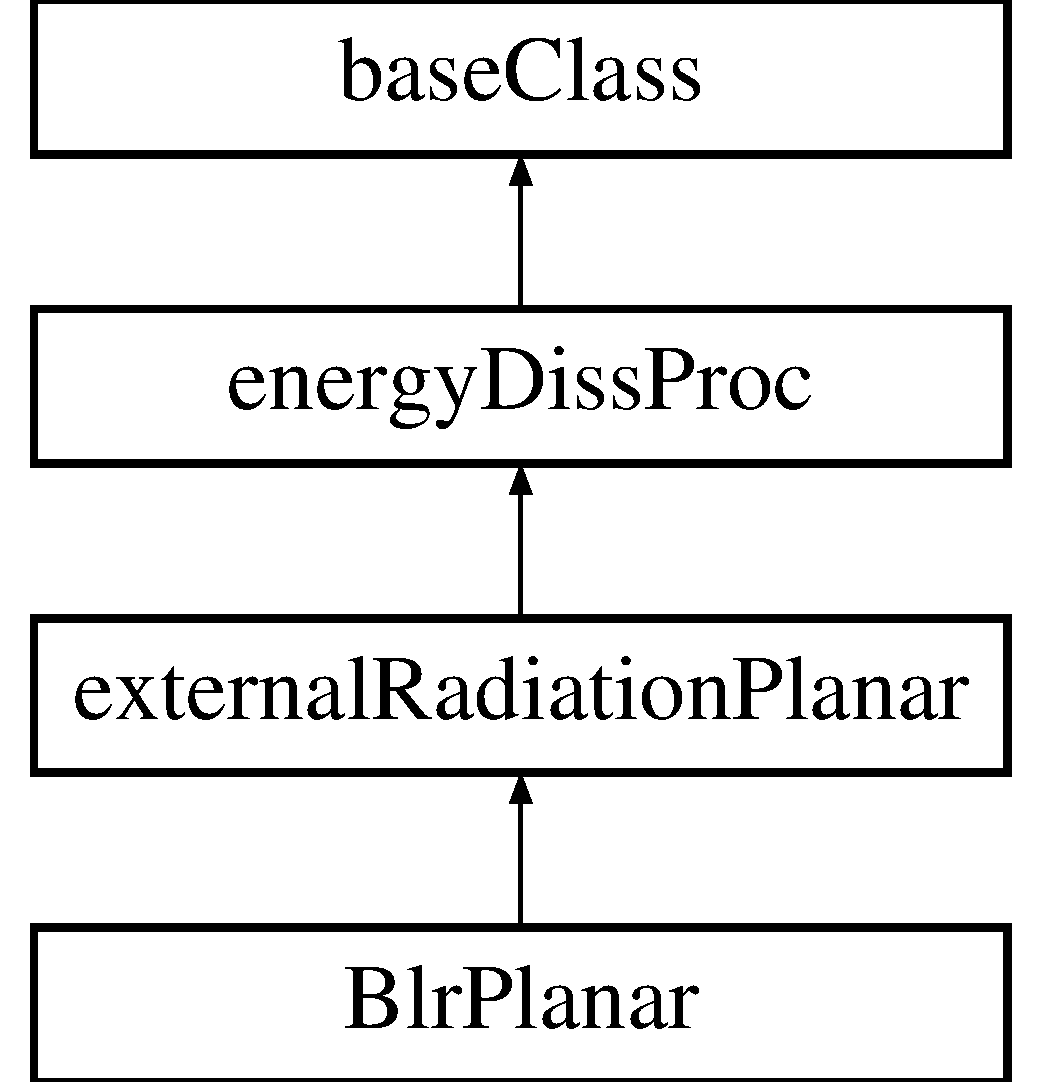
\includegraphics[height=4.000000cm]{classBlrPlanar}
\end{center}
\end{figure}


\subsection{Detailed Description}
Parameters used by class (defaults) 
\begin{DoxyParams}{Parameters}
{\em alpha} & (\hyperlink{classexternalRadiationPlanar}{external\-Radiation\-Planar}) ( alpha = 0.\-0 ) \\
\hline
{\em R1} & -\/ (\hyperlink{classexternalRadiationPlanar}{external\-Radiation\-Planar}) blr lower boundary radius ('N\-E\-W' stratification) (R1 = 0.\-1$\ast$\-R\-\_\-sub) \\
\hline
{\em R2} & -\/ (\hyperlink{classexternalRadiationPlanar}{external\-Radiation\-Planar}) blr upper boundary radius ('N\-E\-W' stratification) (R2 = R\-\_\-sub) \\
\hline
{\em s} & -\/ (\hyperlink{classexternalRadiationPlanar}{external\-Radiation\-Planar}) stratification index ('N\-E\-W' stratification) (s = 2.\-0) \\
\hline
{\em e} & -\/ energy (ext) in e\-V (e = 10.\-0) \\
\hline
{\em C\-F} & -\/ covering factor (C\-F = 0.\-1) \\
\hline
{\em q1} & -\/ lower index in stratification ('M03' stratification) (q1 = 1.\-0) \\
\hline
{\em q2} & -\/ upper index in stratification ('M03' stratification) (q2 = 1.\-0) \\
\hline
{\em Rext} & -\/ blr upper radius ('M03' stratification) (R2 = 0.\-1$\ast$\-R\-\_\-sub) \\
\hline
{\em strat} & -\/ sets stratification ('N\-E\-W' or 'M03') (strat = 'N\-E\-W')\\
\hline
\end{DoxyParams}
Parameters used by class (defaults) 
\begin{DoxyParams}{Parameters}
{\em alpha} & (\hyperlink{classexternalRadiationPlanar}{external\-Radiation\-Planar}) ( alpha = 0.\-0 ) \\
\hline
{\em R1} & -\/ (\hyperlink{classexternalRadiationPlanar}{external\-Radiation\-Planar}) dt lower boundary radius (R1 = R\-\_\-sub) \\
\hline
{\em R2} & -\/ (\hyperlink{classexternalRadiationPlanar}{external\-Radiation\-Planar}) dt upper boundary radius (R2 = 10.\-0$\ast$\-R\-\_\-sub) \\
\hline
{\em s} & -\/ (\hyperlink{classexternalRadiationPlanar}{external\-Radiation\-Planar}) stratification index (s = 1.\-0) \\
\hline
{\em e} & -\/ energy (ext) in e\-V (e = 0.\-6203 @ Rext $\sim$ 1.\-5e14 Hz) \\
\hline
{\em C\-F} & -\/ covering factor (C\-F = 0.\-1) \\
\hline
\end{DoxyParams}
\subsection*{Public Member Functions}
\begin{DoxyCompactItemize}
\item 
\hyperlink{classBlrPlanar_a3c66d1e3ed46fdaf1cf0a14b4eb2000d}{Blr\-Planar} (scfgp $\ast$\-\_\-cfg, \hyperlink{classjetGeometry}{jet\-Geometry} $\ast$\-\_\-r, \hyperlink{classelectrons}{electrons} $\ast$\-\_\-ele, std\-::string \-\_\-id)
\item 
\hyperlink{classBlrPlanar_ab800d81f438dcec82b9d6837b89dddd2}{$\sim$\-Blr\-Planar} ()
\item 
void \hyperlink{classBlrPlanar_a3321d83625869e16c5794d9419dff073}{print\-Info} ()
\item 
void \hyperlink{classBlrPlanar_a549653fdf0d0f5c91a5f5822a5b422c1}{set\-Radius} ()
\item 
double \hyperlink{classBlrPlanar_abe8831b3b2d9ea5d632a354f1305bf86}{getvext} (double \-\_\-\-R)
\item 
void \hyperlink{classBlrPlanar_afcd6617d32754c8377b123317531b613}{setd\-Ld\-R} ()
\end{DoxyCompactItemize}
\subsection*{Additional Inherited Members}


\subsection{Constructor \& Destructor Documentation}
\hypertarget{classBlrPlanar_a3c66d1e3ed46fdaf1cf0a14b4eb2000d}{\index{Blr\-Planar@{Blr\-Planar}!Blr\-Planar@{Blr\-Planar}}
\index{Blr\-Planar@{Blr\-Planar}!BlrPlanar@{Blr\-Planar}}
\subsubsection[{Blr\-Planar}]{\setlength{\rightskip}{0pt plus 5cm}Blr\-Planar\-::\-Blr\-Planar (
\begin{DoxyParamCaption}
\item[{scfgp $\ast$}]{\-\_\-cfg, }
\item[{{\bf jet\-Geometry} $\ast$}]{\-\_\-r, }
\item[{{\bf electrons} $\ast$}]{\-\_\-ele, }
\item[{std\-::string}]{\-\_\-id}
\end{DoxyParamCaption}
)}}\label{classBlrPlanar_a3c66d1e3ed46fdaf1cf0a14b4eb2000d}
constructor 
\begin{DoxyParams}{Parameters}
{\em \-\_\-cfg} & -\/ scfgp class object \\
\hline
{\em \-\_\-r} & -\/ \hyperlink{classjetGeometry}{jet\-Geometry} class object \\
\hline
{\em \-\_\-ele} & -\/ electrons class object \\
\hline
{\em \-\_\-id} & \\
\hline
\end{DoxyParams}

\begin{DoxyCode}
9                                                                                : 
      \hyperlink{classexternalRadiationPlanar_a6254e3256914a093886b7af1f1dc4876}{externalRadiationPlanar}( \hyperlink{classbaseClass_a744f87a6ebe63da08256c022d42a4ca7}{cfg}, \hyperlink{classbaseClass_a482bb9b1d94f3eb3f31026d14e9a2bb6}{r}, \hyperlink{classenergyDissProc_a0dbf0777938131e938c1fdad5df38a7f}{ele}, \textcolor{keywordtype}{id} ) \{
10   \textcolor{comment}{/* request parameters */}
11   \hyperlink{classbaseClass_a744f87a6ebe63da08256c022d42a4ca7}{cfg} -> request<double>( \textcolor{keywordtype}{id}+\textcolor{stringliteral}{"e"}, 10.0, &e );
12   \hyperlink{classbaseClass_a744f87a6ebe63da08256c022d42a4ca7}{cfg} -> request<double>( \textcolor{keywordtype}{id}+\textcolor{stringliteral}{"cf"}, 0.1, &cf );
13   \hyperlink{classbaseClass_a744f87a6ebe63da08256c022d42a4ca7}{cfg} -> request<double>( \textcolor{keywordtype}{id}+\textcolor{stringliteral}{"q1"}, 1.0, &q1 );
14   \hyperlink{classbaseClass_a744f87a6ebe63da08256c022d42a4ca7}{cfg} -> request<double>( \textcolor{keywordtype}{id}+\textcolor{stringliteral}{"q2"}, 1.0, &q2 );
15   \hyperlink{classbaseClass_a744f87a6ebe63da08256c022d42a4ca7}{cfg} -> request<double>( \textcolor{keywordtype}{id}+\textcolor{stringliteral}{"R"}, 0.0, &Rext );
16   \hyperlink{classbaseClass_a744f87a6ebe63da08256c022d42a4ca7}{cfg} -> request<std::string>( \textcolor{keywordtype}{id}+\textcolor{stringliteral}{"Strat"}, \textcolor{stringliteral}{"NEW"}, &strat );
17 
18   \hyperlink{classbaseClass_a744f87a6ebe63da08256c022d42a4ca7}{cfg} -> updateRequests( );
19 
20   \textcolor{keywordflow}{if}( strat == \textcolor{stringliteral}{"NEW"} ) \{
21     \textcolor{keywordflow}{if}( R1 == 0.0 || R2 == 0.0 ) \{ \hyperlink{classBlrPlanar_a549653fdf0d0f5c91a5f5822a5b422c1}{setRadius}( ); \}
22     \textcolor{keywordflow}{else} \{ bazinga::warning(\textcolor{keywordtype}{id},\textcolor{stringliteral}{"Overwritting R1 and R2 values from config file!"}); \}
23   \}
24   \textcolor{keywordflow}{else} \textcolor{keywordflow}{if}( strat == \textcolor{stringliteral}{"M03"} ) \{
25     \textcolor{keywordflow}{if}( Rext == 0.0 ) \{ \hyperlink{classBlrPlanar_a549653fdf0d0f5c91a5f5822a5b422c1}{setRadius}( ); \}
26     \textcolor{keywordflow}{else} \{ bazinga::warning(\textcolor{keywordtype}{id},\textcolor{stringliteral}{"Overwritting Rext value from config file!"}); \}
27   \}
28 
29   \hyperlink{classenergyDissProc_aafedd3c012010a8e8aa34247660fea3b}{vpMin} = 0.01*DSQR( \hyperlink{classenergyDissProc_a0dbf0777938131e938c1fdad5df38a7f}{ele} -> getGammaMin( ) )*\hyperlink{classBlrPlanar_abe8831b3b2d9ea5d632a354f1305bf86}{getvext}( Rext );
30   vpMax = 100.0*DSQR( \hyperlink{classenergyDissProc_a0dbf0777938131e938c1fdad5df38a7f}{ele} -> getGammaMax( ) )*\hyperlink{classBlrPlanar_abe8831b3b2d9ea5d632a354f1305bf86}{getvext}( Rext );
31 
32   \textcolor{comment}{/* initialize disk radius R;}
33 \textcolor{comment}{     here we use N-1 to use the same Upe as in other processes */}
34   R = \textcolor{keyword}{new} \hyperlink{classlogGeometry}{logGeometry}( R1, R2, \hyperlink{classbaseClass_a2b4d07d2b46197d495de0477f4bb22f8}{N}-1 );
35 
36   allocateUpe( ); \textcolor{comment}{// this is for storing matrix information about dUpe(r)/dR (R) }
37   allocateUpeR( ); \textcolor{comment}{// this is for storing vector information about Upe(r) }
38   allocateLpv( );
39   allocateLvPoint( );
40   allocateLvPointAvg( );
41 
42   \textcolor{keywordflow}{for}( \textcolor{keywordtype}{int} i=0;i<\hyperlink{classbaseClass_a2b4d07d2b46197d495de0477f4bb22f8}{N};i++ ) \{ set\_vp( i, \hyperlink{classenergyDissProc_aafedd3c012010a8e8aa34247660fea3b}{vpMin}*pow( vpMax/\hyperlink{classenergyDissProc_aafedd3c012010a8e8aa34247660fea3b}{vpMin},(\textcolor{keywordtype}{double})i/((\textcolor{keywordtype}{double})N-1)) ); \}
43   
44   \textcolor{comment}{/* set the values of dLdR */}
45   \hyperlink{classBlrPlanar_afcd6617d32754c8377b123317531b613}{setdLdR}( ); \}
\end{DoxyCode}
\hypertarget{classBlrPlanar_ab800d81f438dcec82b9d6837b89dddd2}{\index{Blr\-Planar@{Blr\-Planar}!$\sim$\-Blr\-Planar@{$\sim$\-Blr\-Planar}}
\index{$\sim$\-Blr\-Planar@{$\sim$\-Blr\-Planar}!BlrPlanar@{Blr\-Planar}}
\subsubsection[{$\sim$\-Blr\-Planar}]{\setlength{\rightskip}{0pt plus 5cm}Blr\-Planar\-::$\sim$\-Blr\-Planar (
\begin{DoxyParamCaption}
{}
\end{DoxyParamCaption}
)}}\label{classBlrPlanar_ab800d81f438dcec82b9d6837b89dddd2}
destructor 
\begin{DoxyCode}
47                        \{
48   freeUpe( );
49   freeLpv( );
50   freeLvPoint( );
51   freeLvPointAvg( ); \}
\end{DoxyCode}


\subsection{Member Function Documentation}
\hypertarget{classBlrPlanar_abe8831b3b2d9ea5d632a354f1305bf86}{\index{Blr\-Planar@{Blr\-Planar}!getvext@{getvext}}
\index{getvext@{getvext}!BlrPlanar@{Blr\-Planar}}
\subsubsection[{getvext}]{\setlength{\rightskip}{0pt plus 5cm}double Blr\-Planar\-::getvext (
\begin{DoxyParamCaption}
\item[{double}]{\-\_\-\-R}
\end{DoxyParamCaption}
)\hspace{0.3cm}{\ttfamily [virtual]}}}\label{classBlrPlanar_abe8831b3b2d9ea5d632a354f1305bf86}
get v\-\_\-ext value in Hz 
\begin{DoxyParams}{Parameters}
{\em \-\_\-\-R} & -\/ radius in accretion disk plane \\
\hline
\end{DoxyParams}
\begin{DoxyReturn}{Returns}
v\-\_\-ext 
\end{DoxyReturn}


Reimplemented from \hyperlink{classexternalRadiationPlanar_aa9ea7f37d1e43219f71ec6b215a38b96}{external\-Radiation\-Planar}.


\begin{DoxyCode}
115                                      \{
116   vext = e*eV2erg/PLANCK\_H;
117   \textcolor{keywordflow}{return} vext; \}
\end{DoxyCode}
\hypertarget{classBlrPlanar_a3321d83625869e16c5794d9419dff073}{\index{Blr\-Planar@{Blr\-Planar}!print\-Info@{print\-Info}}
\index{print\-Info@{print\-Info}!BlrPlanar@{Blr\-Planar}}
\subsubsection[{print\-Info}]{\setlength{\rightskip}{0pt plus 5cm}void Blr\-Planar\-::print\-Info (
\begin{DoxyParamCaption}
{}
\end{DoxyParamCaption}
)\hspace{0.3cm}{\ttfamily [virtual]}}}\label{classBlrPlanar_a3321d83625869e16c5794d9419dff073}
print basic information about myself (virtual) 

Reimplemented from \hyperlink{classexternalRadiationPlanar_a47e497b12dfa4e71311bffb3a4b384b2}{external\-Radiation\-Planar}.


\begin{DoxyCode}
53                            \{
54   bazinga::info(\textcolor{keywordtype}{id},\textcolor{stringliteral}{"Info"});
55   bazinga::print\_info(\textcolor{keywordtype}{id},\textcolor{stringliteral}{"N"},\hyperlink{classbaseClass_a2b4d07d2b46197d495de0477f4bb22f8}{N});
56   bazinga::print\_info(\textcolor{keywordtype}{id},\textcolor{stringliteral}{"Using stratification version"},strat);
57   \textcolor{keywordflow}{if}( strat == \textcolor{stringliteral}{"NEW"} ) \{
58     bazinga::print\_info(\textcolor{keywordtype}{id},\textcolor{stringliteral}{"radius R1"},R1,\textcolor{stringliteral}{"cm"});
59     bazinga::print\_info(\textcolor{keywordtype}{id},\textcolor{stringliteral}{"radius R2"},R2,\textcolor{stringliteral}{"cm"});
60     bazinga::print\_info(\textcolor{keywordtype}{id},\textcolor{stringliteral}{"stratification index"},s); \}
61   \textcolor{keywordflow}{if}( strat == \textcolor{stringliteral}{"M03"} ) \{
62     bazinga::print\_info(\textcolor{keywordtype}{id},\textcolor{stringliteral}{"radius Rext"},Rext,\textcolor{stringliteral}{"cm"});
63     bazinga::print\_info(\textcolor{keywordtype}{id},\textcolor{stringliteral}{"radius R1"},R1,\textcolor{stringliteral}{"cm"});
64     bazinga::print\_info(\textcolor{keywordtype}{id},\textcolor{stringliteral}{"radius R2"},R2,\textcolor{stringliteral}{"cm"});
65     bazinga::print\_info(\textcolor{keywordtype}{id},\textcolor{stringliteral}{"stratfication index q1"},q1);
66     bazinga::print\_info(\textcolor{keywordtype}{id},\textcolor{stringliteral}{"stratfication index q2"},q2); \}
67   
68   bazinga::print\_info(\textcolor{keywordtype}{id},\textcolor{stringliteral}{"Avg energy (in external frame)"},e,\textcolor{stringliteral}{"eV"});
69   bazinga::print\_info(\textcolor{keywordtype}{id},\textcolor{stringliteral}{"Avg frequency (in external frame)"},\hyperlink{classBlrPlanar_abe8831b3b2d9ea5d632a354f1305bf86}{getvext}( Rext ),\textcolor{stringliteral}{"Hz"});
70   bazinga::print\_info(\textcolor{keywordtype}{id},\textcolor{stringliteral}{"Clouds covering factor cf"},cf);
71   bazinga::print\_info(\textcolor{keywordtype}{id},\textcolor{stringliteral}{"alpha"},alpha);
72   bazinga::print\_info(\textcolor{keywordtype}{id},\textcolor{stringliteral}{"vpMin"},\hyperlink{classenergyDissProc_aafedd3c012010a8e8aa34247660fea3b}{vpMin},\textcolor{stringliteral}{"Hz"});
73   bazinga::print\_info(\textcolor{keywordtype}{id},\textcolor{stringliteral}{"vpMax"},vpMax,\textcolor{stringliteral}{"Hz"});
74   \textcolor{keywordflow}{if}( approx ) \{ bazinga::print\_info(\textcolor{keywordtype}{id},\textcolor{stringliteral}{"Using approximate dependence on R"}); \}
75   \textcolor{keywordflow}{if}( \hyperlink{classenergyDissProc_a2cc4e4eae15982f977a0dfa5458d80f4}{luminosityConstU} ) \{ bazinga::warning(\textcolor{keywordtype}{id},\textcolor{stringliteral}{"Using constant u' to calculate luminosity."}
      ); \}
76   \textcolor{keywordflow}{if}( \hyperlink{classenergyDissProc_a0a23854c1c830dfb9ac33d116fce5b7d}{luminosityConstNu} ) \{ bazinga::warning(\textcolor{keywordtype}{id},\textcolor{stringliteral}{"Using constant v\_ext to calculate
       luminosity."}); \}
77 \}
\end{DoxyCode}
\hypertarget{classBlrPlanar_afcd6617d32754c8377b123317531b613}{\index{Blr\-Planar@{Blr\-Planar}!setd\-Ld\-R@{setd\-Ld\-R}}
\index{setd\-Ld\-R@{setd\-Ld\-R}!BlrPlanar@{Blr\-Planar}}
\subsubsection[{setd\-Ld\-R}]{\setlength{\rightskip}{0pt plus 5cm}void Blr\-Planar\-::setd\-Ld\-R (
\begin{DoxyParamCaption}
{}
\end{DoxyParamCaption}
)\hspace{0.3cm}{\ttfamily [virtual]}}}\label{classBlrPlanar_afcd6617d32754c8377b123317531b613}
set d\-L/d\-R for particulat source 

Reimplemented from \hyperlink{classexternalRadiationPlanar_a7914df2de2d822755ac1c9e6d860e22b}{external\-Radiation\-Planar}.


\begin{DoxyCode}
95                          \{
96   \textcolor{keywordtype}{double} Ledd = 1.3e47*mBH;
97   \textcolor{keywordtype}{double} Ldisk = eDisk*mDot*Ledd;
98   \textcolor{comment}{/* fill in dLdR vector that will be used for the rest of the calculations */}
99   bazinga::info(\textcolor{keywordtype}{id},\textcolor{stringliteral}{"Seeting dLdR."});
100   \textcolor{keywordflow}{for}( \textcolor{keywordtype}{int} i=0;i<R->getMaxIndex();i++ ) \{
101     R -> \hyperlink{classexternalRadiationPlanar_acfddae49394d11c89d1d47229ba8a3f7}{update}( i );
102     \textcolor{keywordtype}{double} val = 0.0;
103     \textcolor{keywordflow}{if}( strat == \textcolor{stringliteral}{"NEW"} ) \{ val = cf*Ldisk*\hyperlink{classexternalRadiationPlanar_a351a13f462898c59bae55ce606829648}{ctau}( )*pow(R->get( ),-s); \}
104     \textcolor{keywordflow}{if}( strat == \textcolor{stringliteral}{"M03"} ) \{ 
105       val = cf*Ldisk/(R->get()*(q1+q2)/(q1*q2));
106       \textcolor{keywordflow}{if}( R->get() <= Rext ) \{ val *= pow(R->get()/Rext,q1); \}
107       \textcolor{keywordflow}{if}( R->get() > Rext ) \{ val *= pow(R->get()/Rext,-q2); \}
108     \}
109     gsl\_vector\_set( dLdR, R->getIndex( ), val );
110   \}
111   \textcolor{comment}{/* Now when we have all set let us save what we have just calculated - dLdR */}
112   bazinga::info(\textcolor{keywordtype}{id},\textcolor{stringliteral}{"Saving dLdR."});
113   bazinga::save\_GSLVector( \textcolor{stringliteral}{"dLdR\_"}+this->\hyperlink{classbaseClass_a756d5accf10ced9a34024048c95a51c9}{whoAmI}( ), R->getRadius\_GSLVector( ), dLdR, 
      \hyperlink{classbaseClass_a744f87a6ebe63da08256c022d42a4ca7}{cfg}->get<std::string>(\textcolor{stringliteral}{"output"}) ); \}
\end{DoxyCode}
\hypertarget{classBlrPlanar_a549653fdf0d0f5c91a5f5822a5b422c1}{\index{Blr\-Planar@{Blr\-Planar}!set\-Radius@{set\-Radius}}
\index{set\-Radius@{set\-Radius}!BlrPlanar@{Blr\-Planar}}
\subsubsection[{set\-Radius}]{\setlength{\rightskip}{0pt plus 5cm}void Blr\-Planar\-::set\-Radius (
\begin{DoxyParamCaption}
{}
\end{DoxyParamCaption}
)\hspace{0.3cm}{\ttfamily [virtual]}}}\label{classBlrPlanar_a549653fdf0d0f5c91a5f5822a5b422c1}
sets rext if not provided by config file 

Reimplemented from \hyperlink{classexternalRadiationPlanar_a710859cda6258d75098ccb31e60ab261}{external\-Radiation\-Planar}.


\begin{DoxyCode}
79                            \{
80   \textcolor{keywordtype}{double} Ledd = 1.3e47*mBH;
81   \textcolor{keywordtype}{double} Ldisk = eDisk*mDot*Ledd;
82   \textcolor{keywordtype}{double} R\_sub = 1.6e-5*sqrt( Ldisk );
83   \textcolor{keywordflow}{if}( strat == \textcolor{stringliteral}{"NEW"} ) \{
84     R1 = 0.1*R\_sub;
85     R2 = R\_sub;
86       \textcolor{comment}{/* Rext is set only to avoid 'if's in constructor when setting vpMIN and vpMAX; Rext is just set to
       R1 */}
87     Rext = R1; \}
88   \textcolor{keywordflow}{else} \textcolor{keywordflow}{if}( strat == \textcolor{stringliteral}{"M03"} ) \{
89     Rext = 0.1*R\_sub;
90     \textcolor{comment}{/* values R1 and r2 in M03 are only bounds for numerical reasons */}
91     R1 = 1.0e-5*R\_sub; \textcolor{comment}{// ???}
92     R2 = 10.0*R\_sub; \}
93 \}
\end{DoxyCode}


The documentation for this class was generated from the following files\-:\begin{DoxyCompactItemize}
\item 
/home/mjaniak/\-Soft/blazar++/include/\hyperlink{BlrPlanar_8hpp}{Blr\-Planar.\-hpp}\item 
/home/mjaniak/\-Soft/blazar++/src/\hyperlink{BlrPlanar_8cpp}{Blr\-Planar.\-cpp}\end{DoxyCompactItemize}

\hypertarget{classBlrSpherical}{\section{Blr\-Spherical Class Reference}
\label{classBlrSpherical}\index{Blr\-Spherical@{Blr\-Spherical}}
}


{\ttfamily \#include $<$Blr\-Spherical.\-hpp$>$}

Inheritance diagram for Blr\-Spherical\-:\begin{figure}[H]
\begin{center}
\leavevmode
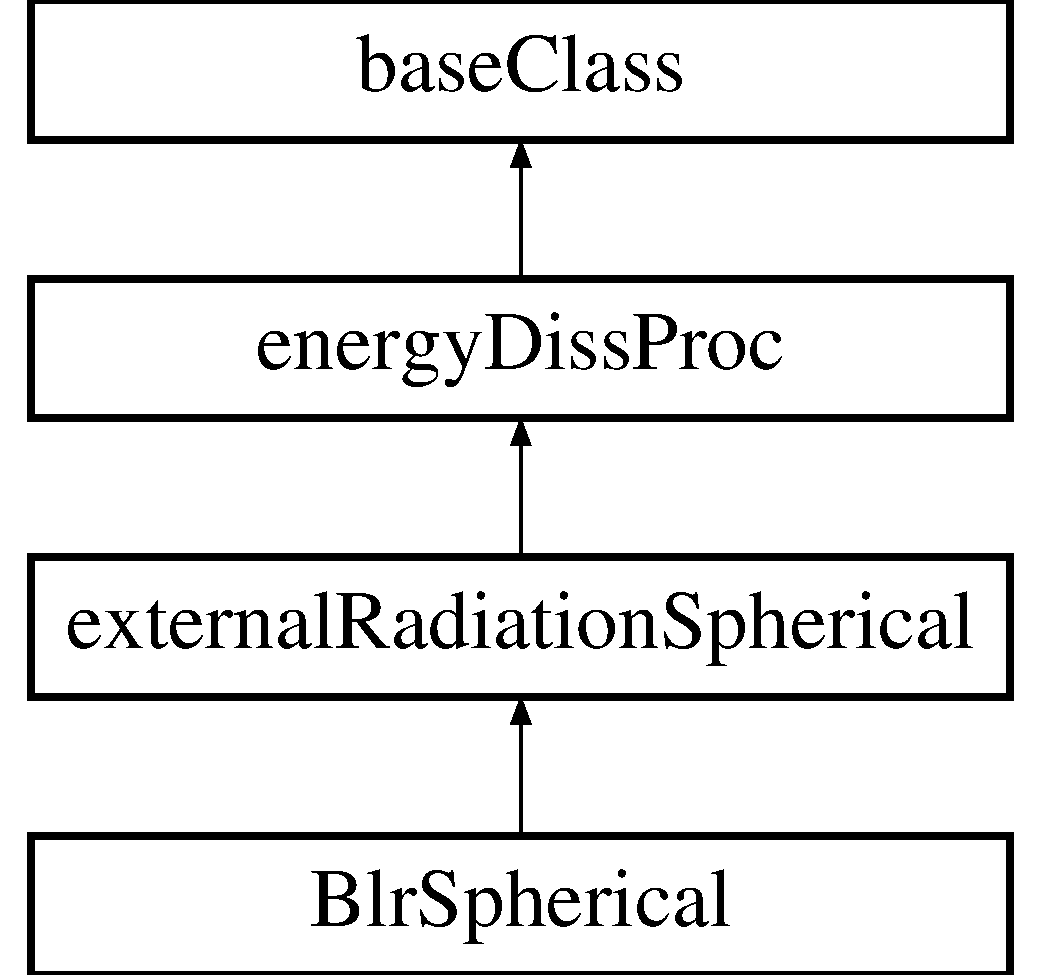
\includegraphics[height=4.000000cm]{classBlrSpherical}
\end{center}
\end{figure}


\subsection{Detailed Description}
Parameters used by class (defaults) 
\begin{DoxyParams}{Parameters}
{\em e} & (\hyperlink{classexternalRadiationSpherical}{external\-Radiation\-Spherical}) -\/ energy (ext) in e\-V (e = 10.\-0) \\
\hline
{\em cf} & (\hyperlink{classexternalRadiationSpherical}{external\-Radiation\-Spherical}) -\/ covering factor (cf = 0.\-1) \\
\hline
{\em q1} & -\/ lower index in stratification (q1 = 1.\-0) \\
\hline
{\em q2} & -\/ upper index in stratification (q2 = 3.\-0) \\
\hline
{\em rext} & -\/ blr radius (rext = 0.\-1$\ast$r\-\_\-sub) \\
\hline
\end{DoxyParams}
\subsection*{Public Member Functions}
\begin{DoxyCompactItemize}
\item 
\hyperlink{classBlrSpherical_aaa33e7d7429aaf2ece12eca0599b4273}{Blr\-Spherical} (scfgp $\ast$\-\_\-cfg, \hyperlink{classjetGeometry}{jet\-Geometry} $\ast$\-\_\-r, \hyperlink{classelectrons}{electrons} $\ast$\-\_\-ele, std\-::string \-\_\-id)
\item 
\hyperlink{classBlrSpherical_a65f7ff9e2207d6558d0ed4ada8a6f049}{$\sim$\-Blr\-Spherical} ()
\item 
void \hyperlink{classBlrSpherical_ad67ab24f0b7f0ec3a0893fd2e3170f6c}{update} ()
\item 
void \hyperlink{classBlrSpherical_a101b95271855f15f1049fcea9efde235}{print\-Info} ()
\item 
void \hyperlink{classBlrSpherical_adc2876b14e36b86f5a35d31c708d5d35}{set\-Radius} ()
\item 
double \hyperlink{classBlrSpherical_aaf00f59d04b5e193aa47959dd1cc1065}{getvext} (double \-\_\-r)
\end{DoxyCompactItemize}
\subsection*{Additional Inherited Members}


\subsection{Constructor \& Destructor Documentation}
\hypertarget{classBlrSpherical_aaa33e7d7429aaf2ece12eca0599b4273}{\index{Blr\-Spherical@{Blr\-Spherical}!Blr\-Spherical@{Blr\-Spherical}}
\index{Blr\-Spherical@{Blr\-Spherical}!BlrSpherical@{Blr\-Spherical}}
\subsubsection[{Blr\-Spherical}]{\setlength{\rightskip}{0pt plus 5cm}Blr\-Spherical\-::\-Blr\-Spherical (
\begin{DoxyParamCaption}
\item[{scfgp $\ast$}]{\-\_\-cfg, }
\item[{{\bf jet\-Geometry} $\ast$}]{\-\_\-r, }
\item[{{\bf electrons} $\ast$}]{\-\_\-ele, }
\item[{std\-::string}]{\-\_\-id}
\end{DoxyParamCaption}
)}}\label{classBlrSpherical_aaa33e7d7429aaf2ece12eca0599b4273}
constructor 
\begin{DoxyParams}{Parameters}
{\em \-\_\-cfg} & -\/ scfgp class object \\
\hline
{\em \-\_\-r} & -\/ \hyperlink{classjetGeometry}{jet\-Geometry} class object \\
\hline
{\em \-\_\-ele} & -\/ electrons class object \\
\hline
{\em \-\_\-id} & \\
\hline
\end{DoxyParams}
!! 
\begin{DoxyCode}
9                                                                                      : 
      \hyperlink{classexternalRadiationSpherical_a8bc8c23cc374776d0c4431751dda67ed}{externalRadiationSpherical}( \hyperlink{classbaseClass_a744f87a6ebe63da08256c022d42a4ca7}{cfg}, \hyperlink{classbaseClass_a482bb9b1d94f3eb3f31026d14e9a2bb6}{r}, \hyperlink{classenergyDissProc_a0dbf0777938131e938c1fdad5df38a7f}{ele}, \textcolor{keywordtype}{id} ) \{
10   \textcolor{comment}{/* request parameters */}
11   \hyperlink{classbaseClass_a744f87a6ebe63da08256c022d42a4ca7}{cfg} -> request<double>( \textcolor{keywordtype}{id}+\textcolor{stringliteral}{"q1"}, 1.0, &q1 );
12   \hyperlink{classbaseClass_a744f87a6ebe63da08256c022d42a4ca7}{cfg} -> request<double>( \textcolor{keywordtype}{id}+\textcolor{stringliteral}{"q2"}, 1.0, &q2 );
13   \hyperlink{classbaseClass_a744f87a6ebe63da08256c022d42a4ca7}{cfg} -> request<double>( \textcolor{keywordtype}{id}+\textcolor{stringliteral}{"r"}, 0.0, &rext ); 
14   \hyperlink{classbaseClass_a744f87a6ebe63da08256c022d42a4ca7}{cfg} -> request<double>(\textcolor{stringliteral}{"mBH"},1.0,&mBH);
15   \hyperlink{classbaseClass_a744f87a6ebe63da08256c022d42a4ca7}{cfg} -> request<double>(\textcolor{stringliteral}{"eDisk"},0.1,&eDisk);
16   \hyperlink{classbaseClass_a744f87a6ebe63da08256c022d42a4ca7}{cfg} -> request<double>(\textcolor{stringliteral}{"mDot"},1.0,&mDot);
17   \hyperlink{classbaseClass_a744f87a6ebe63da08256c022d42a4ca7}{cfg} -> request<double>(\textcolor{stringliteral}{"Gamma"},10.0,&Gamma);
18 
19   \hyperlink{classbaseClass_a744f87a6ebe63da08256c022d42a4ca7}{cfg} -> updateRequests( );
20 
21   \textcolor{keywordflow}{if}( rext == 0.0 ) \{ \hyperlink{classBlrSpherical_adc2876b14e36b86f5a35d31c708d5d35}{setRadius}( ); \}
22   \textcolor{keywordflow}{else} \{ bazinga::warning(\textcolor{keywordtype}{id},\textcolor{stringliteral}{"Overwritting rext value from config file!"}); \}
23 
24   \hyperlink{classenergyDissProc_aafedd3c012010a8e8aa34247660fea3b}{vpMin} = 0.01*DSQR( \hyperlink{classenergyDissProc_a0dbf0777938131e938c1fdad5df38a7f}{ele} -> getGammaMin() )*\hyperlink{classBlrSpherical_aaf00f59d04b5e193aa47959dd1cc1065}{getvext}( rext );
25   vpMax = 100.0*DSQR( \hyperlink{classenergyDissProc_a0dbf0777938131e938c1fdad5df38a7f}{ele} -> getGammaMax() )*\hyperlink{classBlrSpherical_aaf00f59d04b5e193aa47959dd1cc1065}{getvext}( rext );
26 
27   allocateUpe( );
28   allocateLpv( );
29   allocateLvPoint( );
30   allocateLvPointAvg( );
31 
32   \textcolor{keywordflow}{for}( \textcolor{keywordtype}{int} i=0;i<\hyperlink{classbaseClass_a2b4d07d2b46197d495de0477f4bb22f8}{N};i++ ) \{ set\_vp( i, \hyperlink{classenergyDissProc_aafedd3c012010a8e8aa34247660fea3b}{vpMin}*pow( vpMax/\hyperlink{classenergyDissProc_aafedd3c012010a8e8aa34247660fea3b}{vpMin},(\textcolor{keywordtype}{double})i/((\textcolor{keywordtype}{double})N-1)) ); \}
33 \}
\end{DoxyCode}
\hypertarget{classBlrSpherical_a65f7ff9e2207d6558d0ed4ada8a6f049}{\index{Blr\-Spherical@{Blr\-Spherical}!$\sim$\-Blr\-Spherical@{$\sim$\-Blr\-Spherical}}
\index{$\sim$\-Blr\-Spherical@{$\sim$\-Blr\-Spherical}!BlrSpherical@{Blr\-Spherical}}
\subsubsection[{$\sim$\-Blr\-Spherical}]{\setlength{\rightskip}{0pt plus 5cm}Blr\-Spherical\-::$\sim$\-Blr\-Spherical (
\begin{DoxyParamCaption}
{}
\end{DoxyParamCaption}
)\hspace{0.3cm}{\ttfamily [inline]}}}\label{classBlrSpherical_a65f7ff9e2207d6558d0ed4ada8a6f049}
destructor 
\begin{DoxyCode}
39 \{ \}
\end{DoxyCode}


\subsection{Member Function Documentation}
\hypertarget{classBlrSpherical_aaf00f59d04b5e193aa47959dd1cc1065}{\index{Blr\-Spherical@{Blr\-Spherical}!getvext@{getvext}}
\index{getvext@{getvext}!BlrSpherical@{Blr\-Spherical}}
\subsubsection[{getvext}]{\setlength{\rightskip}{0pt plus 5cm}double Blr\-Spherical\-::getvext (
\begin{DoxyParamCaption}
\item[{double}]{\-\_\-r}
\end{DoxyParamCaption}
)\hspace{0.3cm}{\ttfamily [virtual]}}}\label{classBlrSpherical_aaf00f59d04b5e193aa47959dd1cc1065}
get v\-\_\-ext value in Hz 
\begin{DoxyParams}{Parameters}
{\em \-\_\-r} & -\/ radius \\
\hline
\end{DoxyParams}
\begin{DoxyReturn}{Returns}
v\-\_\-ext 
\end{DoxyReturn}


Reimplemented from \hyperlink{classexternalRadiationSpherical_a444023a18bd55023dc806bd0acccb7a0}{external\-Radiation\-Spherical}.


\begin{DoxyCode}
65                                         \{
66   vext = e*eV2erg/PLANCK\_H;
67   \textcolor{keywordflow}{return} vext; \}
\end{DoxyCode}
\hypertarget{classBlrSpherical_a101b95271855f15f1049fcea9efde235}{\index{Blr\-Spherical@{Blr\-Spherical}!print\-Info@{print\-Info}}
\index{print\-Info@{print\-Info}!BlrSpherical@{Blr\-Spherical}}
\subsubsection[{print\-Info}]{\setlength{\rightskip}{0pt plus 5cm}void Blr\-Spherical\-::print\-Info (
\begin{DoxyParamCaption}
{}
\end{DoxyParamCaption}
)\hspace{0.3cm}{\ttfamily [virtual]}}}\label{classBlrSpherical_a101b95271855f15f1049fcea9efde235}
print basic information about myself (virtual) 

Reimplemented from \hyperlink{classexternalRadiationSpherical_a232684df0d246d8c5ec06e832bbaad0f}{external\-Radiation\-Spherical}.


\begin{DoxyCode}
35                               \{
36   bazinga::info(\textcolor{keywordtype}{id},\textcolor{stringliteral}{"Info"});
37   bazinga::print\_info(\textcolor{keywordtype}{id},\textcolor{stringliteral}{"N"},\hyperlink{classbaseClass_a2b4d07d2b46197d495de0477f4bb22f8}{N});
38   bazinga::print\_info(\textcolor{keywordtype}{id},\textcolor{stringliteral}{"Avg energy (in external frame)"},e,\textcolor{stringliteral}{"eV"});
39   bazinga::print\_info(\textcolor{keywordtype}{id},\textcolor{stringliteral}{"Avg frequency (in external frame)"},\hyperlink{classBlrSpherical_aaf00f59d04b5e193aa47959dd1cc1065}{getvext}( rext ),\textcolor{stringliteral}{"Hz"});
40   bazinga::print\_info(\textcolor{keywordtype}{id},\textcolor{stringliteral}{"Clouds covering factor cf"},cf);
41   bazinga::print\_info(\textcolor{keywordtype}{id},\textcolor{stringliteral}{"radius r"},rext,\textcolor{stringliteral}{"cm"});
42   bazinga::print\_info(\textcolor{keywordtype}{id},\textcolor{stringliteral}{"q1"},q1);
43   bazinga::print\_info(\textcolor{keywordtype}{id},\textcolor{stringliteral}{"q2"},q2);
44   bazinga::print\_info(\textcolor{keywordtype}{id},\textcolor{stringliteral}{"vpMin"},\hyperlink{classenergyDissProc_aafedd3c012010a8e8aa34247660fea3b}{vpMin},\textcolor{stringliteral}{"Hz"});
45   bazinga::print\_info(\textcolor{keywordtype}{id},\textcolor{stringliteral}{"vpMax"},vpMax,\textcolor{stringliteral}{"Hz"});
46   \textcolor{keywordflow}{if}( \hyperlink{classenergyDissProc_a2cc4e4eae15982f977a0dfa5458d80f4}{luminosityConstU} ) \{ bazinga::warning(\textcolor{keywordtype}{id},\textcolor{stringliteral}{"Using constant u' to calculate luminosity."}
      ); \}
47 \}
\end{DoxyCode}
\hypertarget{classBlrSpherical_adc2876b14e36b86f5a35d31c708d5d35}{\index{Blr\-Spherical@{Blr\-Spherical}!set\-Radius@{set\-Radius}}
\index{set\-Radius@{set\-Radius}!BlrSpherical@{Blr\-Spherical}}
\subsubsection[{set\-Radius}]{\setlength{\rightskip}{0pt plus 5cm}void Blr\-Spherical\-::set\-Radius (
\begin{DoxyParamCaption}
{}
\end{DoxyParamCaption}
)\hspace{0.3cm}{\ttfamily [virtual]}}}\label{classBlrSpherical_adc2876b14e36b86f5a35d31c708d5d35}
sets rext if not provided by config file 

Reimplemented from \hyperlink{classexternalRadiationSpherical_a560bd33ee97e6bdc7dc0d6138705e9b3}{external\-Radiation\-Spherical}.


\begin{DoxyCode}
49                               \{
50   \textcolor{keywordtype}{double} Ledd = 1.3e47*mBH;
51   \textcolor{keywordtype}{double} Ldisk = eDisk*mDot*Ledd;
52   \textcolor{keywordtype}{double} R\_sub = 1.6e-5*sqrt(Ldisk);
53   rext = 0.1*R\_sub; \}
\end{DoxyCode}
\hypertarget{classBlrSpherical_ad67ab24f0b7f0ec3a0893fd2e3170f6c}{\index{Blr\-Spherical@{Blr\-Spherical}!update@{update}}
\index{update@{update}!BlrSpherical@{Blr\-Spherical}}
\subsubsection[{update}]{\setlength{\rightskip}{0pt plus 5cm}void Blr\-Spherical\-::update (
\begin{DoxyParamCaption}
{}
\end{DoxyParamCaption}
)\hspace{0.3cm}{\ttfamily [virtual]}}}\label{classBlrSpherical_ad67ab24f0b7f0ec3a0893fd2e3170f6c}
calculate and set Upe every time with new radius r 

Reimplemented from \hyperlink{classexternalRadiationSpherical_a05f5cf91c3a3c7844b167ff4476e64f8}{external\-Radiation\-Spherical}.


\begin{DoxyCode}
69                             \{
70   \textcolor{keywordtype}{double} Ledd = 1.3e47*mBH;
71   \textcolor{keywordtype}{double} Ldisk = eDisk*mDot*Ledd;
72   \textcolor{keywordtype}{double} u\_ext = Gamma*Gamma*cf*Ldisk/(6.*M\_PI*LIGHT\_SPEED*rext*rext);
73   \textcolor{keywordflow}{if}( \hyperlink{classbaseClass_a482bb9b1d94f3eb3f31026d14e9a2bb6}{r}->get( ) <= rext ) \{ u\_ext *= pow( \hyperlink{classbaseClass_a482bb9b1d94f3eb3f31026d14e9a2bb6}{r}->get( )/rext, -q1 ); \}
74   \textcolor{keywordflow}{if}( \hyperlink{classbaseClass_a482bb9b1d94f3eb3f31026d14e9a2bb6}{r}->get( ) > rext ) \{ u\_ext *= pow( \hyperlink{classbaseClass_a482bb9b1d94f3eb3f31026d14e9a2bb6}{r}->get( )/rext, -q2 ); \}
75   gsl\_vector\_set( upe, \hyperlink{classbaseClass_a482bb9b1d94f3eb3f31026d14e9a2bb6}{r}->getIndex( ), u\_ext );
76   bazinga::print\_info(\textcolor{keywordtype}{id},\textcolor{stringliteral}{"Upe"},gsl\_vector\_get( upe, \hyperlink{classbaseClass_a482bb9b1d94f3eb3f31026d14e9a2bb6}{r}->getIndex( ) ) );
77   set\_upe\_r( gsl\_vector\_get( upe, \hyperlink{classbaseClass_a482bb9b1d94f3eb3f31026d14e9a2bb6}{r}->getIndex( ) ) );
78   \hyperlink{classenergyDissProc_a7b51925f603e271657cab66afe822591}{flag\_upe\_r} = \textcolor{keyword}{false}; \}
\end{DoxyCode}


The documentation for this class was generated from the following files\-:\begin{DoxyCompactItemize}
\item 
/home/mjaniak/\-Soft/blazar++/include/\hyperlink{BlrSpherical_8hpp}{Blr\-Spherical.\-hpp}\item 
/home/mjaniak/\-Soft/blazar++/src/\hyperlink{BlrSpherical_8cpp}{Blr\-Spherical.\-cpp}\end{DoxyCompactItemize}

\hypertarget{classBlrSphericalGu}{\section{Blr\-Spherical\-Gu Class Reference}
\label{classBlrSphericalGu}\index{Blr\-Spherical\-Gu@{Blr\-Spherical\-Gu}}
}


{\ttfamily \#include $<$Blr\-Spherical\-Gu.\-hpp$>$}

Inheritance diagram for Blr\-Spherical\-Gu\-:\begin{figure}[H]
\begin{center}
\leavevmode
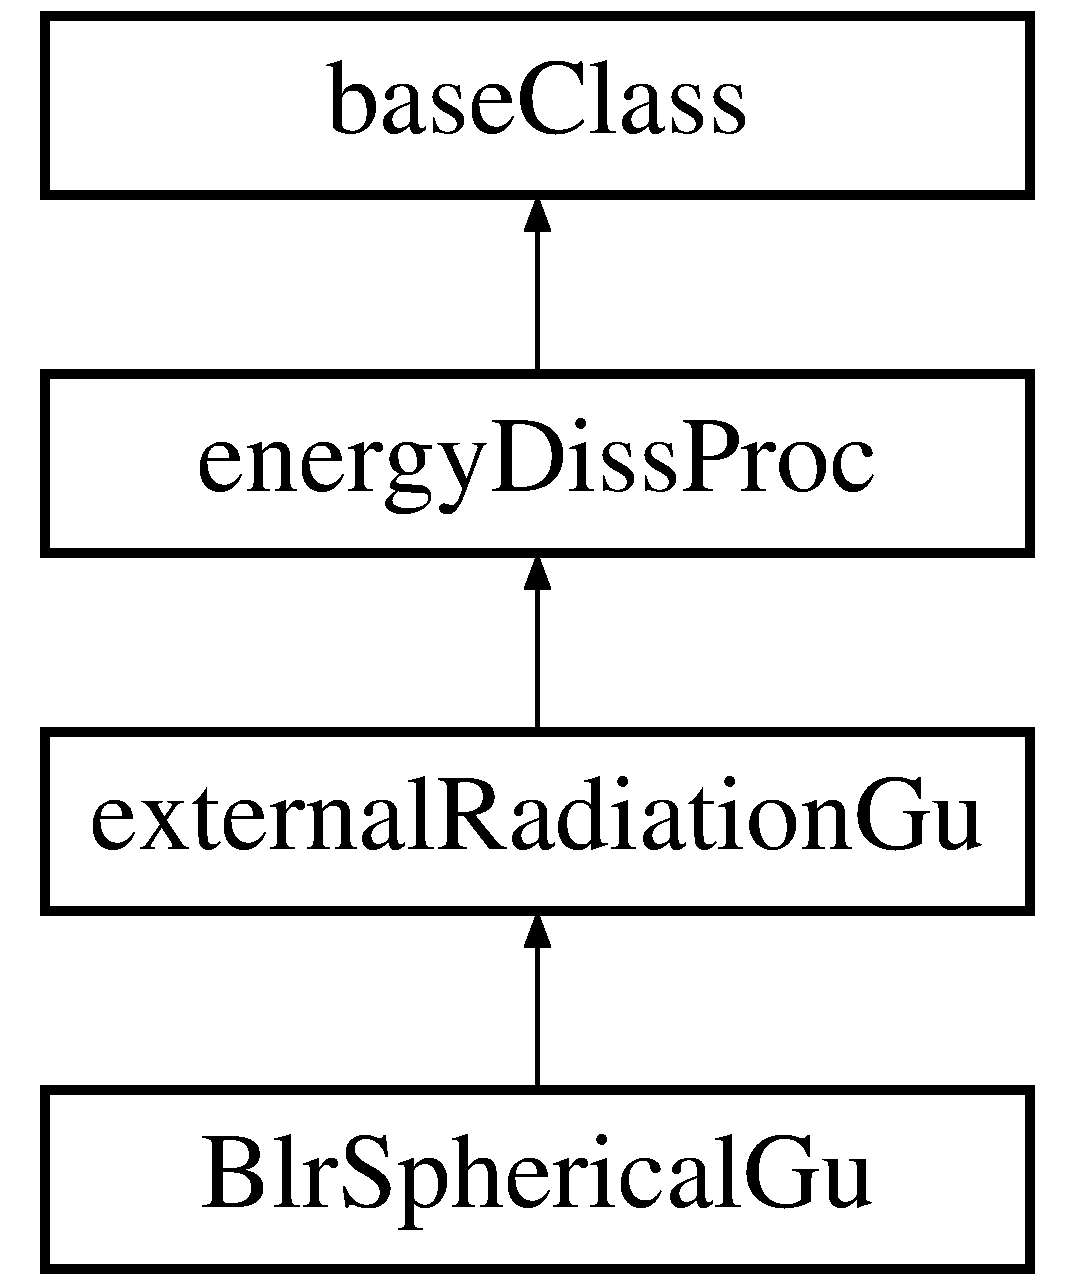
\includegraphics[height=4.000000cm]{classBlrSphericalGu}
\end{center}
\end{figure}


\subsection{Detailed Description}
Parameters used by class (defaults) 
\begin{DoxyParams}{Parameters}
{\em e} & (\hyperlink{classexternalRadiationGu}{external\-Radiation\-Gu}) -\/ energy (ext) in e\-V (e = 10.\-0) \\
\hline
{\em cf} & (external\-Radiation\-Spherical\-Gu) -\/ covering factor (cf = 0.\-1) \\
\hline
{\em rext} & -\/ blr radius (rext = 0.\-1$\ast$r\-\_\-sub) \\
\hline
{\em k} & -\/ u\-\_\-ext vs r index = 3 \\
\hline
\end{DoxyParams}
\subsection*{Public Member Functions}
\begin{DoxyCompactItemize}
\item 
\hyperlink{classBlrSphericalGu_a297b6bef804d5653ab02a7534e233334}{Blr\-Spherical\-Gu} (scfgp $\ast$\-\_\-cfg, \hyperlink{classjetGeometry}{jet\-Geometry} $\ast$\-\_\-r, \hyperlink{classelectrons}{electrons} $\ast$\-\_\-ele, std\-::string \-\_\-id)
\item 
\hyperlink{classBlrSphericalGu_ac65ecb74330a83910937e67712170e0f}{$\sim$\-Blr\-Spherical\-Gu} ()
\item 
void \hyperlink{classBlrSphericalGu_a69de552417b7b01c3634650aaa9413d7}{print\-Info} ()
\item 
void \hyperlink{classBlrSphericalGu_a0054a1bc21351e6d68b8b5190ab1a8b0}{update} ()
\item 
double \hyperlink{classBlrSphericalGu_a78d8a3ace3f41082c48df04ea01bc142}{getvext} (double \-\_\-r)
\item 
void \hyperlink{classBlrSphericalGu_a51161abb05542e2120756bbdba82fc0b}{set\-Radius} ()
\end{DoxyCompactItemize}
\subsection*{Additional Inherited Members}


\subsection{Constructor \& Destructor Documentation}
\hypertarget{classBlrSphericalGu_a297b6bef804d5653ab02a7534e233334}{\index{Blr\-Spherical\-Gu@{Blr\-Spherical\-Gu}!Blr\-Spherical\-Gu@{Blr\-Spherical\-Gu}}
\index{Blr\-Spherical\-Gu@{Blr\-Spherical\-Gu}!BlrSphericalGu@{Blr\-Spherical\-Gu}}
\subsubsection[{Blr\-Spherical\-Gu}]{\setlength{\rightskip}{0pt plus 5cm}Blr\-Spherical\-Gu\-::\-Blr\-Spherical\-Gu (
\begin{DoxyParamCaption}
\item[{scfgp $\ast$}]{\-\_\-cfg, }
\item[{{\bf jet\-Geometry} $\ast$}]{\-\_\-r, }
\item[{{\bf electrons} $\ast$}]{\-\_\-ele, }
\item[{std\-::string}]{\-\_\-id}
\end{DoxyParamCaption}
)}}\label{classBlrSphericalGu_a297b6bef804d5653ab02a7534e233334}
constructor 
\begin{DoxyParams}{Parameters}
{\em \-\_\-cfg} & -\/ scfgp class object \\
\hline
{\em \-\_\-r} & -\/ \hyperlink{classjetGeometry}{jet\-Geometry} class object \\
\hline
{\em \-\_\-ele} & -\/ electrons class object \\
\hline
{\em \-\_\-id} & \\
\hline
\end{DoxyParams}

\begin{DoxyCode}
9                                                                                          : 
      \hyperlink{classexternalRadiationGu_aad5903b642f08594be10d699cf9fb3b4}{externalRadiationGu}( \hyperlink{classbaseClass_a744f87a6ebe63da08256c022d42a4ca7}{cfg}, \hyperlink{classbaseClass_a482bb9b1d94f3eb3f31026d14e9a2bb6}{r}, \hyperlink{classenergyDissProc_a0dbf0777938131e938c1fdad5df38a7f}{ele}, \textcolor{keywordtype}{id} ) \{
10   \textcolor{comment}{/* requested parameters */}
11   \hyperlink{classbaseClass_a744f87a6ebe63da08256c022d42a4ca7}{cfg} -> request<double>(\textcolor{keywordtype}{id} + \textcolor{stringliteral}{"e"}, 10.0, &e );
12   \hyperlink{classbaseClass_a744f87a6ebe63da08256c022d42a4ca7}{cfg} -> request<double>(\textcolor{keywordtype}{id} + \textcolor{stringliteral}{"cf"}, 0.1, &cf );
13   \hyperlink{classbaseClass_a744f87a6ebe63da08256c022d42a4ca7}{cfg} -> request<double>(\textcolor{keywordtype}{id} + \textcolor{stringliteral}{"rext"}, 0.0, &rext );
14   \hyperlink{classbaseClass_a744f87a6ebe63da08256c022d42a4ca7}{cfg} -> request<double>(\textcolor{keywordtype}{id} + \textcolor{stringliteral}{"k"}, 3.0, &k );
15 
16   \hyperlink{classbaseClass_a744f87a6ebe63da08256c022d42a4ca7}{cfg} -> updateRequests( );
17 
18   \textcolor{keywordflow}{if}( rext == 0.0 ) \{ \hyperlink{classBlrSphericalGu_a51161abb05542e2120756bbdba82fc0b}{setRadius}( ); \}
19   \textcolor{keywordflow}{else} \{ bazinga::warning(\textcolor{keywordtype}{id},\textcolor{stringliteral}{"Overwritting rext value from config file!"}); \}
20   
21   \hyperlink{classenergyDissProc_aafedd3c012010a8e8aa34247660fea3b}{vpMin} = 0.01*DSQR( \hyperlink{classenergyDissProc_a0dbf0777938131e938c1fdad5df38a7f}{ele} -> getGammaMin( ) )*\hyperlink{classBlrSphericalGu_a78d8a3ace3f41082c48df04ea01bc142}{getvext}( \hyperlink{classbaseClass_a482bb9b1d94f3eb3f31026d14e9a2bb6}{r}->getRMax() );
22   vpMax = 100.0*DSQR( \hyperlink{classenergyDissProc_a0dbf0777938131e938c1fdad5df38a7f}{ele} -> getGammaMax( ) )*\hyperlink{classBlrSphericalGu_a78d8a3ace3f41082c48df04ea01bc142}{getvext}( \hyperlink{classbaseClass_a482bb9b1d94f3eb3f31026d14e9a2bb6}{r}->getR0() );
23 
24   allocateUpeR( ); \textcolor{comment}{// this is for storing vector information about Upe(r) }
25   allocateLpv( );
26   allocateLvPoint( );
27   allocateLvPointAvg( );
28 
29   \textcolor{keywordflow}{for}( \textcolor{keywordtype}{int} i=0;i<\hyperlink{classbaseClass_a2b4d07d2b46197d495de0477f4bb22f8}{N};i++ ) \{ set\_vp( i, \hyperlink{classenergyDissProc_aafedd3c012010a8e8aa34247660fea3b}{vpMin}*pow( vpMax/\hyperlink{classenergyDissProc_aafedd3c012010a8e8aa34247660fea3b}{vpMin},(\textcolor{keywordtype}{double})i/((\textcolor{keywordtype}{double})N-1)) ); \}
30 \}
\end{DoxyCode}
\hypertarget{classBlrSphericalGu_ac65ecb74330a83910937e67712170e0f}{\index{Blr\-Spherical\-Gu@{Blr\-Spherical\-Gu}!$\sim$\-Blr\-Spherical\-Gu@{$\sim$\-Blr\-Spherical\-Gu}}
\index{$\sim$\-Blr\-Spherical\-Gu@{$\sim$\-Blr\-Spherical\-Gu}!BlrSphericalGu@{Blr\-Spherical\-Gu}}
\subsubsection[{$\sim$\-Blr\-Spherical\-Gu}]{\setlength{\rightskip}{0pt plus 5cm}Blr\-Spherical\-Gu\-::$\sim$\-Blr\-Spherical\-Gu (
\begin{DoxyParamCaption}
{}
\end{DoxyParamCaption}
)\hspace{0.3cm}{\ttfamily [inline]}}}\label{classBlrSphericalGu_ac65ecb74330a83910937e67712170e0f}
destructor 
\begin{DoxyCode}
35 \{ \}
\end{DoxyCode}


\subsection{Member Function Documentation}
\hypertarget{classBlrSphericalGu_a78d8a3ace3f41082c48df04ea01bc142}{\index{Blr\-Spherical\-Gu@{Blr\-Spherical\-Gu}!getvext@{getvext}}
\index{getvext@{getvext}!BlrSphericalGu@{Blr\-Spherical\-Gu}}
\subsubsection[{getvext}]{\setlength{\rightskip}{0pt plus 5cm}double Blr\-Spherical\-Gu\-::getvext (
\begin{DoxyParamCaption}
\item[{double}]{\-\_\-r}
\end{DoxyParamCaption}
)\hspace{0.3cm}{\ttfamily [virtual]}}}\label{classBlrSphericalGu_a78d8a3ace3f41082c48df04ea01bc142}
get v\-\_\-ext value in Hz 
\begin{DoxyParams}{Parameters}
{\em \-\_\-r} & -\/ radius \\
\hline
\end{DoxyParams}
\begin{DoxyReturn}{Returns}
v\-\_\-ext 
\end{DoxyReturn}


Reimplemented from \hyperlink{classexternalRadiationGu_ab7e1abcc40cf0538404e88a0febdfb02}{external\-Radiation\-Gu}.


\begin{DoxyCode}
32 \{ \textcolor{keywordflow}{return} e*eV2erg/PLANCK\_H; \}
\end{DoxyCode}
\hypertarget{classBlrSphericalGu_a69de552417b7b01c3634650aaa9413d7}{\index{Blr\-Spherical\-Gu@{Blr\-Spherical\-Gu}!print\-Info@{print\-Info}}
\index{print\-Info@{print\-Info}!BlrSphericalGu@{Blr\-Spherical\-Gu}}
\subsubsection[{print\-Info}]{\setlength{\rightskip}{0pt plus 5cm}void Blr\-Spherical\-Gu\-::print\-Info (
\begin{DoxyParamCaption}
{}
\end{DoxyParamCaption}
)\hspace{0.3cm}{\ttfamily [virtual]}}}\label{classBlrSphericalGu_a69de552417b7b01c3634650aaa9413d7}
print basic information about myself (virtual) 

Reimplemented from \hyperlink{classexternalRadiationGu_a8aa28d939b0ecf2651f18cc4f5f6ba25}{external\-Radiation\-Gu}.


\begin{DoxyCode}
47                                 \{
48   bazinga::info(\textcolor{keywordtype}{id},\textcolor{stringliteral}{"Info"});
49   bazinga::print\_info(\textcolor{keywordtype}{id},\textcolor{stringliteral}{"N"},\hyperlink{classbaseClass_a2b4d07d2b46197d495de0477f4bb22f8}{N});
50   bazinga::print\_info(\textcolor{keywordtype}{id},\textcolor{stringliteral}{"Avg energy (in external frame)"},e,\textcolor{stringliteral}{"eV"});
51   bazinga::print\_info(\textcolor{keywordtype}{id},\textcolor{stringliteral}{"Avg frequency (in external frame)"},\hyperlink{classBlrSphericalGu_a78d8a3ace3f41082c48df04ea01bc142}{getvext}( \hyperlink{classbaseClass_a482bb9b1d94f3eb3f31026d14e9a2bb6}{r}->getR0()),\textcolor{stringliteral}{"Hz"});
52   bazinga::print\_info(\textcolor{keywordtype}{id},\textcolor{stringliteral}{"Clouds covering factor cf"},cf);
53   bazinga::print\_info(\textcolor{keywordtype}{id},\textcolor{stringliteral}{"radius rext"},rext,\textcolor{stringliteral}{"cm"});
54   bazinga::print\_info(\textcolor{keywordtype}{id},\textcolor{stringliteral}{"strat index k"},k);
55   bazinga::print\_info(\textcolor{keywordtype}{id},\textcolor{stringliteral}{"vpMin"},\hyperlink{classenergyDissProc_aafedd3c012010a8e8aa34247660fea3b}{vpMin},\textcolor{stringliteral}{"Hz"});
56   bazinga::print\_info(\textcolor{keywordtype}{id},\textcolor{stringliteral}{"vpMax"},vpMax,\textcolor{stringliteral}{"Hz"});
57 \}
\end{DoxyCode}
\hypertarget{classBlrSphericalGu_a51161abb05542e2120756bbdba82fc0b}{\index{Blr\-Spherical\-Gu@{Blr\-Spherical\-Gu}!set\-Radius@{set\-Radius}}
\index{set\-Radius@{set\-Radius}!BlrSphericalGu@{Blr\-Spherical\-Gu}}
\subsubsection[{set\-Radius}]{\setlength{\rightskip}{0pt plus 5cm}void Blr\-Spherical\-Gu\-::set\-Radius (
\begin{DoxyParamCaption}
{}
\end{DoxyParamCaption}
)\hspace{0.3cm}{\ttfamily [virtual]}}}\label{classBlrSphericalGu_a51161abb05542e2120756bbdba82fc0b}
sets rext if not provided by config file 

Reimplemented from \hyperlink{classexternalRadiationGu_a541b2bb7da733f10d83af6225b7ad5f8}{external\-Radiation\-Gu}.


\begin{DoxyCode}
59                                  \{
60   \textcolor{keywordtype}{double} Ledd = 1.3e47*mBH;
61   \textcolor{keywordtype}{double} Ldisk = eDisk*mDot*Ledd;
62   \textcolor{keywordtype}{double} R\_sub = 1.6e-5*sqrt( Ldisk );
63   rext = 0.1*R\_sub; \}
\end{DoxyCode}
\hypertarget{classBlrSphericalGu_a0054a1bc21351e6d68b8b5190ab1a8b0}{\index{Blr\-Spherical\-Gu@{Blr\-Spherical\-Gu}!update@{update}}
\index{update@{update}!BlrSphericalGu@{Blr\-Spherical\-Gu}}
\subsubsection[{update}]{\setlength{\rightskip}{0pt plus 5cm}void Blr\-Spherical\-Gu\-::update (
\begin{DoxyParamCaption}
{}
\end{DoxyParamCaption}
)\hspace{0.3cm}{\ttfamily [virtual]}}}\label{classBlrSphericalGu_a0054a1bc21351e6d68b8b5190ab1a8b0}
calculate and set Upe every time with new radius r 

Reimplemented from \hyperlink{classexternalRadiationGu_a730363f393f29aef9927e0bb84087116}{external\-Radiation\-Gu}.


\begin{DoxyCode}
34                               \{
35   \textcolor{keywordtype}{double} Ledd = 1.3e47*mBH;
36   \textcolor{keywordtype}{double} Ldisk = eDisk*mDot*Ledd;
37   \textcolor{keywordtype}{double} temp\_upe = 0.0;
38   \textcolor{keywordtype}{double} temp\_cf = 0.0;
39   temp\_cf = cf;
40   temp\_cf *= pow(\hyperlink{classbaseClass_a482bb9b1d94f3eb3f31026d14e9a2bb6}{r}->get()/rext,2)/(1.0+pow(\hyperlink{classbaseClass_a482bb9b1d94f3eb3f31026d14e9a2bb6}{r}->get()/rext,k));
41   temp\_upe = (temp\_cf*Ldisk*DSQR(Gamma))/(3.0*M\_PI*DSQR(\hyperlink{classbaseClass_a482bb9b1d94f3eb3f31026d14e9a2bb6}{r}->get())*LIGHT\_SPEED);
42   gsl\_vector\_set( \hyperlink{classenergyDissProc_ac925d66519c79f36421f75a6bc9f0965}{upe\_r}, \hyperlink{classbaseClass_a482bb9b1d94f3eb3f31026d14e9a2bb6}{r}->getIndex( ), temp\_upe );
43   bazinga::print\_info(\textcolor{keywordtype}{id},\textcolor{stringliteral}{"Upe"},gsl\_vector\_get( \hyperlink{classenergyDissProc_ac925d66519c79f36421f75a6bc9f0965}{upe\_r}, \hyperlink{classbaseClass_a482bb9b1d94f3eb3f31026d14e9a2bb6}{r}->getIndex( ) ) );
44   set\_upe\_r( gsl\_vector\_get( \hyperlink{classenergyDissProc_ac925d66519c79f36421f75a6bc9f0965}{upe\_r}, \hyperlink{classbaseClass_a482bb9b1d94f3eb3f31026d14e9a2bb6}{r}->getIndex( ) ) );
45   \hyperlink{classenergyDissProc_a7b51925f603e271657cab66afe822591}{flag\_upe\_r} = \textcolor{keyword}{false}; \}
\end{DoxyCode}


The documentation for this class was generated from the following files\-:\begin{DoxyCompactItemize}
\item 
/home/mjaniak/\-Soft/blazar++/include/\hyperlink{BlrSphericalGu_8hpp}{Blr\-Spherical\-Gu.\-hpp}\item 
/home/mjaniak/\-Soft/blazar++/src/\hyperlink{BlrSphericalGu_8cpp}{Blr\-Spherical\-Gu.\-cpp}\end{DoxyCompactItemize}

\hypertarget{classDtPlanar}{\section{Dt\-Planar Class Reference}
\label{classDtPlanar}\index{Dt\-Planar@{Dt\-Planar}}
}
Inheritance diagram for Dt\-Planar\-:\begin{figure}[H]
\begin{center}
\leavevmode
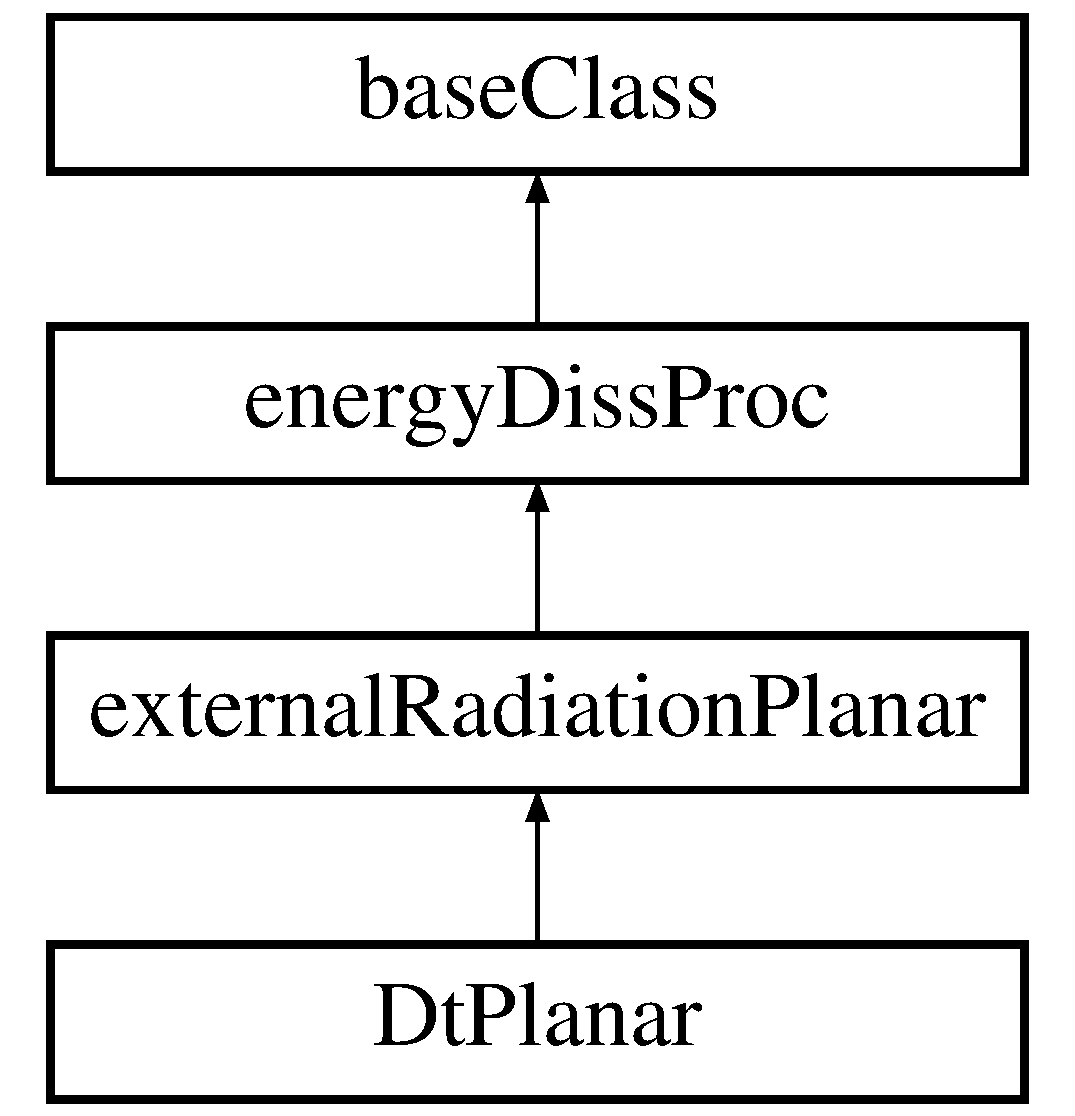
\includegraphics[height=4.000000cm]{classDtPlanar}
\end{center}
\end{figure}
\subsection*{Public Member Functions}
\begin{DoxyCompactItemize}
\item 
\hyperlink{classDtPlanar_a5d5b77f9362b9dccca97df093cf96ab2}{Dt\-Planar} (scfgp $\ast$\-\_\-cfg, \hyperlink{classjetGeometry}{jet\-Geometry} $\ast$\-\_\-r, \hyperlink{classelectrons}{electrons} $\ast$\-\_\-ele, std\-::string \-\_\-id)
\item 
\hyperlink{classDtPlanar_a5ce5e082dab0dbeea9b11c2fae22cfb8}{$\sim$\-Dt\-Planar} ()
\item 
void \hyperlink{classDtPlanar_a0d1b6697d54a08030ed50b7e4b5fbfef}{print\-Info} ()
\item 
void \hyperlink{classDtPlanar_aaa8956b3aa5b8ecff5e746a8ba84a67c}{set\-Radius} ()
\item 
double \hyperlink{classDtPlanar_a46eb0e18c9a391adccffe2623dd3dfbe}{getvext} (double \-\_\-\-R)
\item 
void \hyperlink{classDtPlanar_a6445269d74ae176c5d299ac71cd7ac87}{setd\-Ld\-R} ()
\end{DoxyCompactItemize}
\subsection*{Additional Inherited Members}


\subsection{Constructor \& Destructor Documentation}
\hypertarget{classDtPlanar_a5d5b77f9362b9dccca97df093cf96ab2}{\index{Dt\-Planar@{Dt\-Planar}!Dt\-Planar@{Dt\-Planar}}
\index{Dt\-Planar@{Dt\-Planar}!DtPlanar@{Dt\-Planar}}
\subsubsection[{Dt\-Planar}]{\setlength{\rightskip}{0pt plus 5cm}Dt\-Planar\-::\-Dt\-Planar (
\begin{DoxyParamCaption}
\item[{scfgp $\ast$}]{\-\_\-cfg, }
\item[{{\bf jet\-Geometry} $\ast$}]{\-\_\-r, }
\item[{{\bf electrons} $\ast$}]{\-\_\-ele, }
\item[{std\-::string}]{\-\_\-id}
\end{DoxyParamCaption}
)}}\label{classDtPlanar_a5d5b77f9362b9dccca97df093cf96ab2}
constructor 
\begin{DoxyParams}{Parameters}
{\em \-\_\-cfg} & -\/ scfgp class object \\
\hline
{\em \-\_\-r} & -\/ \hyperlink{classjetGeometry}{jet\-Geometry} class object \\
\hline
{\em \-\_\-ele} & -\/ electrons class object \\
\hline
{\em \-\_\-id} & \\
\hline
\end{DoxyParams}

\begin{DoxyCode}
9                                                                              : 
      \hyperlink{classexternalRadiationPlanar_a6254e3256914a093886b7af1f1dc4876}{externalRadiationPlanar}( \hyperlink{classbaseClass_a744f87a6ebe63da08256c022d42a4ca7}{cfg}, \hyperlink{classbaseClass_a482bb9b1d94f3eb3f31026d14e9a2bb6}{r}, \hyperlink{classenergyDissProc_a0dbf0777938131e938c1fdad5df38a7f}{ele}, \textcolor{keywordtype}{id} ) \{
10   \textcolor{comment}{/* request parameters */}
11   \hyperlink{classbaseClass_a744f87a6ebe63da08256c022d42a4ca7}{cfg} -> request<double>( \textcolor{keywordtype}{id}+\textcolor{stringliteral}{"e"}, 10.0, &e );
12   \hyperlink{classbaseClass_a744f87a6ebe63da08256c022d42a4ca7}{cfg} -> request<double>( \textcolor{keywordtype}{id}+\textcolor{stringliteral}{"cf"}, 0.1, &cf );
13 
14   \hyperlink{classbaseClass_a744f87a6ebe63da08256c022d42a4ca7}{cfg} -> updateRequests( );
15   
16   \textcolor{keywordflow}{if}( R1 == 0.0 || R2 == 0.0 ) \{ \hyperlink{classDtPlanar_aaa8956b3aa5b8ecff5e746a8ba84a67c}{setRadius}( ); \}
17   \textcolor{keywordflow}{else} \{ bazinga::warning(\textcolor{keywordtype}{id},\textcolor{stringliteral}{"Overwritting R1 and R2 values from config file!"}); \}
18   
19   \hyperlink{classenergyDissProc_aafedd3c012010a8e8aa34247660fea3b}{vpMin} = 0.01*DSQR( \hyperlink{classenergyDissProc_a0dbf0777938131e938c1fdad5df38a7f}{ele} -> getGammaMin( ) )*\hyperlink{classDtPlanar_a46eb0e18c9a391adccffe2623dd3dfbe}{getvext}( R2 );
20   vpMax = 100.0*DSQR( \hyperlink{classenergyDissProc_a0dbf0777938131e938c1fdad5df38a7f}{ele} -> getGammaMax( ) )*\hyperlink{classDtPlanar_a46eb0e18c9a391adccffe2623dd3dfbe}{getvext}( R1 );
21 
22   \textcolor{comment}{/* initialize disk radius R;}
23 \textcolor{comment}{     here we use N-1 to use the same Upe as in other processes */}
24   R = \textcolor{keyword}{new} \hyperlink{classlogGeometry}{logGeometry}( R1, R2, \hyperlink{classbaseClass_a2b4d07d2b46197d495de0477f4bb22f8}{N}-1 );
25 
26   allocateUpe( ); \textcolor{comment}{// this is for storing matrix information about dUpe(r)/dR (R) }
27   allocateUpeR( ); \textcolor{comment}{// this is for storing vector information about Upe(r) }
28   allocateLpv( );
29   allocateLvPoint( );
30   allocateLvPointAvg( );
31 
32   \textcolor{keywordflow}{for}( \textcolor{keywordtype}{int} i=0;i<\hyperlink{classbaseClass_a2b4d07d2b46197d495de0477f4bb22f8}{N};i++ ) \{ set\_vp( i, \hyperlink{classenergyDissProc_aafedd3c012010a8e8aa34247660fea3b}{vpMin}*pow( vpMax/\hyperlink{classenergyDissProc_aafedd3c012010a8e8aa34247660fea3b}{vpMin},(\textcolor{keywordtype}{double})i/((\textcolor{keywordtype}{double})N-1)) ); \}
33 
34   \textcolor{comment}{/* set the values of dLdR */}
35   \hyperlink{classDtPlanar_a6445269d74ae176c5d299ac71cd7ac87}{setdLdR}( ); \}
\end{DoxyCode}
\hypertarget{classDtPlanar_a5ce5e082dab0dbeea9b11c2fae22cfb8}{\index{Dt\-Planar@{Dt\-Planar}!$\sim$\-Dt\-Planar@{$\sim$\-Dt\-Planar}}
\index{$\sim$\-Dt\-Planar@{$\sim$\-Dt\-Planar}!DtPlanar@{Dt\-Planar}}
\subsubsection[{$\sim$\-Dt\-Planar}]{\setlength{\rightskip}{0pt plus 5cm}Dt\-Planar\-::$\sim$\-Dt\-Planar (
\begin{DoxyParamCaption}
{}
\end{DoxyParamCaption}
)}}\label{classDtPlanar_a5ce5e082dab0dbeea9b11c2fae22cfb8}
destructor 
\begin{DoxyCode}
37                      \{
38   freeUpe( );
39   freeLpv( );
40   freeLvPoint( );
41   freeLvPointAvg( ); \}
\end{DoxyCode}


\subsection{Member Function Documentation}
\hypertarget{classDtPlanar_a46eb0e18c9a391adccffe2623dd3dfbe}{\index{Dt\-Planar@{Dt\-Planar}!getvext@{getvext}}
\index{getvext@{getvext}!DtPlanar@{Dt\-Planar}}
\subsubsection[{getvext}]{\setlength{\rightskip}{0pt plus 5cm}double Dt\-Planar\-::getvext (
\begin{DoxyParamCaption}
\item[{double}]{\-\_\-\-R}
\end{DoxyParamCaption}
)\hspace{0.3cm}{\ttfamily [virtual]}}}\label{classDtPlanar_a46eb0e18c9a391adccffe2623dd3dfbe}
get v\-\_\-ext value in Hz 
\begin{DoxyParams}{Parameters}
{\em \-\_\-\-R} & -\/ radius in accretion disk plane \\
\hline
\end{DoxyParams}
\begin{DoxyReturn}{Returns}
v\-\_\-ext 
\end{DoxyReturn}


Reimplemented from \hyperlink{classexternalRadiationPlanar_aa9ea7f37d1e43219f71ec6b215a38b96}{external\-Radiation\-Planar}.


\begin{DoxyCode}
82                                     \{
83   vext = e*eV2erg/PLANCK\_H;
84   \textcolor{keywordflow}{if}( \hyperlink{classenergyDissProc_a0a23854c1c830dfb9ac33d116fce5b7d}{luminosityConstNu} ) \{ \textcolor{keywordflow}{return} vext; \}
85   \textcolor{keywordflow}{else} \{ \textcolor{keywordflow}{return} vext*R1/\_R; \}
86 \}
\end{DoxyCode}
\hypertarget{classDtPlanar_a0d1b6697d54a08030ed50b7e4b5fbfef}{\index{Dt\-Planar@{Dt\-Planar}!print\-Info@{print\-Info}}
\index{print\-Info@{print\-Info}!DtPlanar@{Dt\-Planar}}
\subsubsection[{print\-Info}]{\setlength{\rightskip}{0pt plus 5cm}void Dt\-Planar\-::print\-Info (
\begin{DoxyParamCaption}
{}
\end{DoxyParamCaption}
)\hspace{0.3cm}{\ttfamily [virtual]}}}\label{classDtPlanar_a0d1b6697d54a08030ed50b7e4b5fbfef}
print basic information about myself (virtual) 

Reimplemented from \hyperlink{classexternalRadiationPlanar_a47e497b12dfa4e71311bffb3a4b384b2}{external\-Radiation\-Planar}.


\begin{DoxyCode}
43                           \{
44   bazinga::info(\textcolor{keywordtype}{id},\textcolor{stringliteral}{"Info"});
45   bazinga::print\_info(\textcolor{keywordtype}{id},\textcolor{stringliteral}{"N"},\hyperlink{classbaseClass_a2b4d07d2b46197d495de0477f4bb22f8}{N});
46   bazinga::info(\textcolor{keywordtype}{id},\textcolor{stringliteral}{"Using stratification version NEW (only option)"});
47   bazinga::print\_info(\textcolor{keywordtype}{id},\textcolor{stringliteral}{"radius R1"},R1,\textcolor{stringliteral}{"cm"});
48   bazinga::print\_info(\textcolor{keywordtype}{id},\textcolor{stringliteral}{"radius R2"},R2,\textcolor{stringliteral}{"cm"});
49   bazinga::print\_info(\textcolor{keywordtype}{id},\textcolor{stringliteral}{"stratification index"},s);
50   bazinga::print\_info(\textcolor{keywordtype}{id},\textcolor{stringliteral}{"Avg energy (in external frame)"},e,\textcolor{stringliteral}{"eV"});
51   bazinga::print\_info(\textcolor{keywordtype}{id},\textcolor{stringliteral}{"Avg frequency (in external frame)"},\hyperlink{classDtPlanar_a46eb0e18c9a391adccffe2623dd3dfbe}{getvext}( R1 ),\textcolor{stringliteral}{"Hz"});
52   bazinga::print\_info(\textcolor{keywordtype}{id},\textcolor{stringliteral}{"Clouds covering factor cf"},cf);
53   bazinga::print\_info(\textcolor{keywordtype}{id},\textcolor{stringliteral}{"alpha"},alpha);
54   bazinga::print\_info(\textcolor{keywordtype}{id},\textcolor{stringliteral}{"vpMin"},\hyperlink{classenergyDissProc_aafedd3c012010a8e8aa34247660fea3b}{vpMin},\textcolor{stringliteral}{"Hz"});
55   bazinga::print\_info(\textcolor{keywordtype}{id},\textcolor{stringliteral}{"vpMax"},vpMax,\textcolor{stringliteral}{"Hz"});
56   \textcolor{keywordflow}{if}( approx ) \{ bazinga::info(\textcolor{keywordtype}{id},\textcolor{stringliteral}{"Using approximate dependence on R"}); \}
57   \textcolor{keywordflow}{if}( \hyperlink{classenergyDissProc_a2cc4e4eae15982f977a0dfa5458d80f4}{luminosityConstU} ) \{ bazinga::warning(\textcolor{keywordtype}{id},\textcolor{stringliteral}{"Using constant u' to calculate luminosity."}
      ); \}
58   \textcolor{keywordflow}{if}( \hyperlink{classenergyDissProc_a0a23854c1c830dfb9ac33d116fce5b7d}{luminosityConstNu} ) \{ bazinga::warning(\textcolor{keywordtype}{id},\textcolor{stringliteral}{"Using constant v\_ext to calculate
       luminosity."}); \}
59 \}
\end{DoxyCode}
\hypertarget{classDtPlanar_a6445269d74ae176c5d299ac71cd7ac87}{\index{Dt\-Planar@{Dt\-Planar}!setd\-Ld\-R@{setd\-Ld\-R}}
\index{setd\-Ld\-R@{setd\-Ld\-R}!DtPlanar@{Dt\-Planar}}
\subsubsection[{setd\-Ld\-R}]{\setlength{\rightskip}{0pt plus 5cm}void Dt\-Planar\-::setd\-Ld\-R (
\begin{DoxyParamCaption}
{}
\end{DoxyParamCaption}
)\hspace{0.3cm}{\ttfamily [virtual]}}}\label{classDtPlanar_a6445269d74ae176c5d299ac71cd7ac87}
set d\-L/d\-R for particulat source 

Reimplemented from \hyperlink{classexternalRadiationPlanar_a7914df2de2d822755ac1c9e6d860e22b}{external\-Radiation\-Planar}.


\begin{DoxyCode}
68                         \{
69   \textcolor{keywordtype}{double} Ledd = 1.3e47*mBH;
70   \textcolor{keywordtype}{double} Ldisk = eDisk*mDot*Ledd;
71   \textcolor{comment}{/* fill in dLdR vector that will be used for the rest of the calculations */}
72   bazinga::info(\textcolor{keywordtype}{id},\textcolor{stringliteral}{"Seeting dLdR."});
73   \textcolor{keywordflow}{for}( \textcolor{keywordtype}{int} i=0;i<R->getMaxIndex();i++ ) \{
74       R -> \hyperlink{classexternalRadiationPlanar_acfddae49394d11c89d1d47229ba8a3f7}{update}( i );
75       \textcolor{keywordtype}{double} val = 0.0;
76       val = cf*Ldisk*\hyperlink{classexternalRadiationPlanar_a351a13f462898c59bae55ce606829648}{ctau}( )*pow(R->get( ),-s);
77       gsl\_vector\_set( dLdR, R->getIndex(), val ); \}
78   \textcolor{comment}{/* Now when we have all set let us save what we have just calculated - dLdR */}
79   bazinga::info(\textcolor{keywordtype}{id},\textcolor{stringliteral}{"Saving dLdR."});
80   bazinga::save\_GSLVector( \textcolor{stringliteral}{"dLdR\_"}+this->\hyperlink{classbaseClass_a756d5accf10ced9a34024048c95a51c9}{whoAmI}( ), R->getRadius\_GSLVector( ), dLdR, 
      \hyperlink{classbaseClass_a744f87a6ebe63da08256c022d42a4ca7}{cfg}->get<std::string>(\textcolor{stringliteral}{"output"}) ); \}
\end{DoxyCode}
\hypertarget{classDtPlanar_aaa8956b3aa5b8ecff5e746a8ba84a67c}{\index{Dt\-Planar@{Dt\-Planar}!set\-Radius@{set\-Radius}}
\index{set\-Radius@{set\-Radius}!DtPlanar@{Dt\-Planar}}
\subsubsection[{set\-Radius}]{\setlength{\rightskip}{0pt plus 5cm}void Dt\-Planar\-::set\-Radius (
\begin{DoxyParamCaption}
{}
\end{DoxyParamCaption}
)\hspace{0.3cm}{\ttfamily [virtual]}}}\label{classDtPlanar_aaa8956b3aa5b8ecff5e746a8ba84a67c}
sets rext if not provided by config file 

Reimplemented from \hyperlink{classexternalRadiationPlanar_a710859cda6258d75098ccb31e60ab261}{external\-Radiation\-Planar}.


\begin{DoxyCode}
61                           \{
62   \textcolor{keywordtype}{double} Ledd = 1.3e47*mBH;
63   \textcolor{keywordtype}{double} Ldisk = eDisk*mDot*Ledd;
64   \textcolor{keywordtype}{double} R\_sub = 1.6e-5*sqrt( Ldisk );
65   R1 = R\_sub;
66   R2 = 10.0*R\_sub; \}
\end{DoxyCode}


The documentation for this class was generated from the following files\-:\begin{DoxyCompactItemize}
\item 
/home/mjaniak/\-Soft/blazar++/include/\hyperlink{DtPlanar_8hpp}{Dt\-Planar.\-hpp}\item 
/home/mjaniak/\-Soft/blazar++/src/\hyperlink{DtPlanar_8cpp}{Dt\-Planar.\-cpp}\end{DoxyCompactItemize}

\hypertarget{classDtSpherical}{\section{Dt\-Spherical Class Reference}
\label{classDtSpherical}\index{Dt\-Spherical@{Dt\-Spherical}}
}


{\ttfamily \#include $<$Dt\-Spherical.\-hpp$>$}

Inheritance diagram for Dt\-Spherical\-:\begin{figure}[H]
\begin{center}
\leavevmode
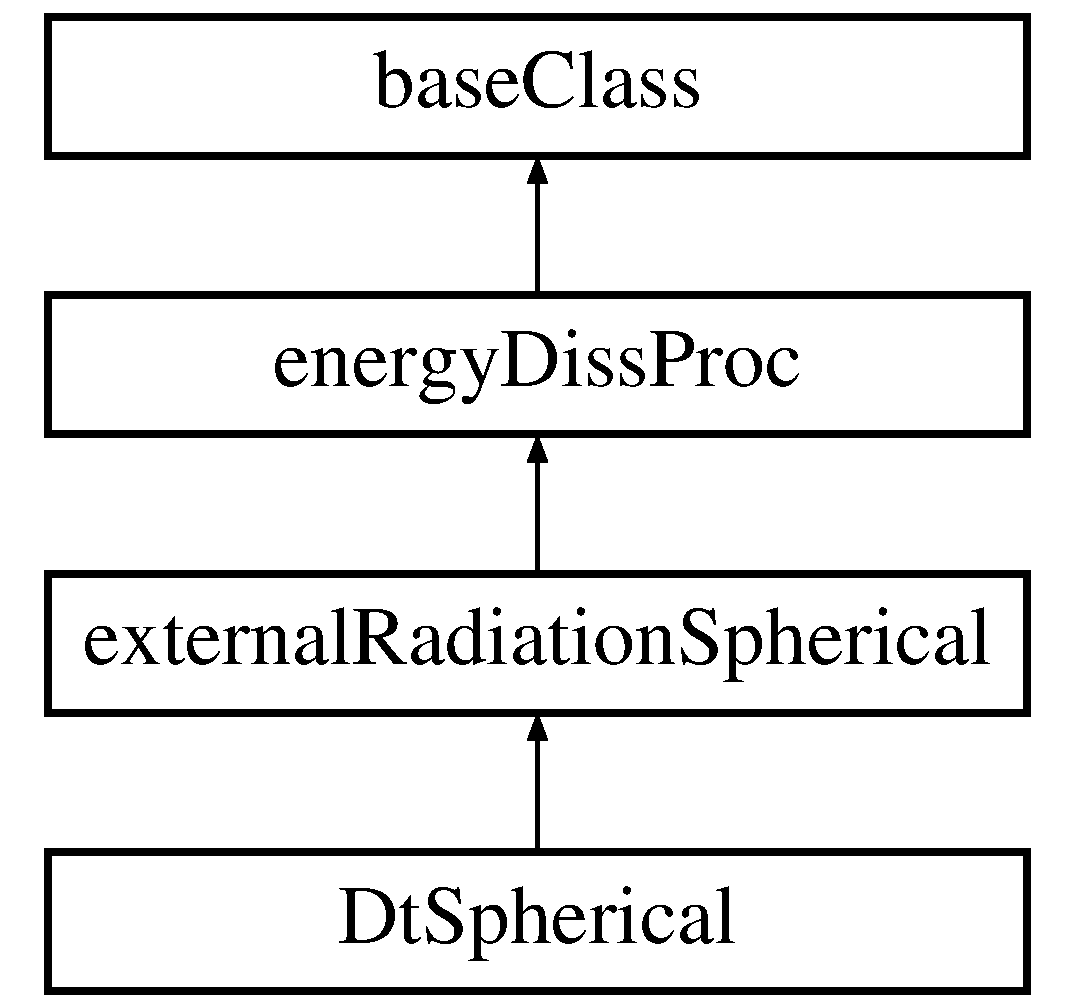
\includegraphics[height=4.000000cm]{classDtSpherical}
\end{center}
\end{figure}


\subsection{Detailed Description}
Parameters used by class (defaults) 
\begin{DoxyParams}{Parameters}
{\em e} & (\hyperlink{classexternalRadiationSpherical}{external\-Radiation\-Spherical}) -\/ energy (ext) in e\-V (e = 0.\-4136 which corresponds to 1.\-5e14\-Hz @ rext) \\
\hline
{\em cf} & (\hyperlink{classexternalRadiationSpherical}{external\-Radiation\-Spherical}) -\/ covering factor (cf = 0.\-1) \\
\hline
{\em q1} & -\/ lower index in stratification (q1 = 0.\-0) \\
\hline
{\em q2} & -\/ upper index in stratification (q2 = -\/3.\-0) \\
\hline
{\em rext} & -\/ dt radius (rext = 1.\-0$\ast$r\-\_\-sub) \\
\hline
\end{DoxyParams}
\subsection*{Public Member Functions}
\begin{DoxyCompactItemize}
\item 
\hyperlink{classDtSpherical_a5699a7154d5b512c254ce7bf63d0735f}{Dt\-Spherical} (scfgp $\ast$\-\_\-cfg, \hyperlink{classjetGeometry}{jet\-Geometry} $\ast$\-\_\-r, \hyperlink{classelectrons}{electrons} $\ast$\-\_\-ele, std\-::string \-\_\-id)
\item 
\hyperlink{classDtSpherical_a936d890404936b9aac665554f7b1ae0d}{$\sim$\-Dt\-Spherical} ()
\item 
void \hyperlink{classDtSpherical_ab9844cfdd3df5bc213bf93dd7b320bb7}{update} ()
\item 
void \hyperlink{classDtSpherical_a14440ec30b997fe2461c07f4507dd994}{print\-Info} ()
\item 
void \hyperlink{classDtSpherical_aac1ed31d84f539e4e372bc1a567e4555}{set\-Radius} ()
\item 
double \hyperlink{classDtSpherical_a25a9bd3b5a47e2d1428325614686f5ac}{getvext} (double \-\_\-r)
\end{DoxyCompactItemize}
\subsection*{Additional Inherited Members}


\subsection{Constructor \& Destructor Documentation}
\hypertarget{classDtSpherical_a5699a7154d5b512c254ce7bf63d0735f}{\index{Dt\-Spherical@{Dt\-Spherical}!Dt\-Spherical@{Dt\-Spherical}}
\index{Dt\-Spherical@{Dt\-Spherical}!DtSpherical@{Dt\-Spherical}}
\subsubsection[{Dt\-Spherical}]{\setlength{\rightskip}{0pt plus 5cm}Dt\-Spherical\-::\-Dt\-Spherical (
\begin{DoxyParamCaption}
\item[{scfgp $\ast$}]{\-\_\-cfg, }
\item[{{\bf jet\-Geometry} $\ast$}]{\-\_\-r, }
\item[{{\bf electrons} $\ast$}]{\-\_\-ele, }
\item[{std\-::string}]{\-\_\-id}
\end{DoxyParamCaption}
)}}\label{classDtSpherical_a5699a7154d5b512c254ce7bf63d0735f}
constructor 
\begin{DoxyParams}{Parameters}
{\em \-\_\-cfg} & -\/ scfgp class object \\
\hline
{\em \-\_\-r} & -\/ \hyperlink{classjetGeometry}{jet\-Geometry} class object \\
\hline
{\em \-\_\-ele} & -\/ electrons class object \\
\hline
{\em \-\_\-id} & \\
\hline
\end{DoxyParams}

\begin{DoxyCode}
9                                                                                    : 
      \hyperlink{classexternalRadiationSpherical_a8bc8c23cc374776d0c4431751dda67ed}{externalRadiationSpherical}( \hyperlink{classbaseClass_a744f87a6ebe63da08256c022d42a4ca7}{cfg}, \hyperlink{classbaseClass_a482bb9b1d94f3eb3f31026d14e9a2bb6}{r}, \hyperlink{classenergyDissProc_a0dbf0777938131e938c1fdad5df38a7f}{ele}, \textcolor{keywordtype}{id} ) \{
10   \textcolor{comment}{/* request parameters */}
11   \hyperlink{classbaseClass_a744f87a6ebe63da08256c022d42a4ca7}{cfg} -> request<double>( \textcolor{keywordtype}{id}+\textcolor{stringliteral}{"q1"}, 1.0, &q1 );
12   \hyperlink{classbaseClass_a744f87a6ebe63da08256c022d42a4ca7}{cfg} -> request<double>( \textcolor{keywordtype}{id}+\textcolor{stringliteral}{"q2"}, 1.0, &q2 );
13   \hyperlink{classbaseClass_a744f87a6ebe63da08256c022d42a4ca7}{cfg} -> request<double>( \textcolor{keywordtype}{id}+\textcolor{stringliteral}{"r"}, 0.0, &rext );
14   \hyperlink{classbaseClass_a744f87a6ebe63da08256c022d42a4ca7}{cfg} -> request<double>(\textcolor{stringliteral}{"mBH"},1.0,&mBH);
15   \hyperlink{classbaseClass_a744f87a6ebe63da08256c022d42a4ca7}{cfg} -> request<double>(\textcolor{stringliteral}{"eDisk"},0.1,&eDisk);
16   \hyperlink{classbaseClass_a744f87a6ebe63da08256c022d42a4ca7}{cfg} -> request<double>(\textcolor{stringliteral}{"mDot"},1.0,&mDot);
17   \hyperlink{classbaseClass_a744f87a6ebe63da08256c022d42a4ca7}{cfg} -> request<double>(\textcolor{stringliteral}{"Gamma"},10.0,&Gamma);
18 
19   \hyperlink{classbaseClass_a744f87a6ebe63da08256c022d42a4ca7}{cfg} -> updateRequests( );
20 
21   \textcolor{keywordflow}{if}( rext == 0.0 ) \{ \hyperlink{classDtSpherical_aac1ed31d84f539e4e372bc1a567e4555}{setRadius}( ); \}
22   \textcolor{keywordflow}{else} \{ bazinga::warning(\textcolor{keywordtype}{id},\textcolor{stringliteral}{"Overwritting rext value from config file!"}); \} 
23 
24   \hyperlink{classenergyDissProc_aafedd3c012010a8e8aa34247660fea3b}{vpMin} = 0.01*DSQR( \hyperlink{classenergyDissProc_a0dbf0777938131e938c1fdad5df38a7f}{ele} -> getGammaMin() )*\hyperlink{classDtSpherical_a25a9bd3b5a47e2d1428325614686f5ac}{getvext}( 10.*rext );
25   vpMax = 100.0*DSQR( \hyperlink{classenergyDissProc_a0dbf0777938131e938c1fdad5df38a7f}{ele} -> getGammaMax() )*\hyperlink{classDtSpherical_a25a9bd3b5a47e2d1428325614686f5ac}{getvext}( rext );
26 
27   allocateUpe( );
28   allocateLpv( );
29   allocateLvPoint( );
30   allocateLvPointAvg( );
31 
32   \textcolor{keywordflow}{for}( \textcolor{keywordtype}{int} i=0;i<\hyperlink{classbaseClass_a2b4d07d2b46197d495de0477f4bb22f8}{N};i++ ) \{ set\_vp( i, \hyperlink{classenergyDissProc_aafedd3c012010a8e8aa34247660fea3b}{vpMin}*pow( vpMax/\hyperlink{classenergyDissProc_aafedd3c012010a8e8aa34247660fea3b}{vpMin},(\textcolor{keywordtype}{double})i/((\textcolor{keywordtype}{double})N-1)) ); \}
33 \}
\end{DoxyCode}
\hypertarget{classDtSpherical_a936d890404936b9aac665554f7b1ae0d}{\index{Dt\-Spherical@{Dt\-Spherical}!$\sim$\-Dt\-Spherical@{$\sim$\-Dt\-Spherical}}
\index{$\sim$\-Dt\-Spherical@{$\sim$\-Dt\-Spherical}!DtSpherical@{Dt\-Spherical}}
\subsubsection[{$\sim$\-Dt\-Spherical}]{\setlength{\rightskip}{0pt plus 5cm}Dt\-Spherical\-::$\sim$\-Dt\-Spherical (
\begin{DoxyParamCaption}
{}
\end{DoxyParamCaption}
)\hspace{0.3cm}{\ttfamily [inline]}}}\label{classDtSpherical_a936d890404936b9aac665554f7b1ae0d}
destructor 
\begin{DoxyCode}
45 \{ \}
\end{DoxyCode}


\subsection{Member Function Documentation}
\hypertarget{classDtSpherical_a25a9bd3b5a47e2d1428325614686f5ac}{\index{Dt\-Spherical@{Dt\-Spherical}!getvext@{getvext}}
\index{getvext@{getvext}!DtSpherical@{Dt\-Spherical}}
\subsubsection[{getvext}]{\setlength{\rightskip}{0pt plus 5cm}double Dt\-Spherical\-::getvext (
\begin{DoxyParamCaption}
\item[{double}]{\-\_\-r}
\end{DoxyParamCaption}
)\hspace{0.3cm}{\ttfamily [virtual]}}}\label{classDtSpherical_a25a9bd3b5a47e2d1428325614686f5ac}
get v\-\_\-ext value in Hz 
\begin{DoxyParams}{Parameters}
{\em \-\_\-r} & -\/ radius \\
\hline
\end{DoxyParams}
\begin{DoxyReturn}{Returns}
v\-\_\-ext 
\end{DoxyReturn}


Reimplemented from \hyperlink{classexternalRadiationSpherical_a444023a18bd55023dc806bd0acccb7a0}{external\-Radiation\-Spherical}.


\begin{DoxyCode}
74                                        \{
75   vext = e*eV2erg/PLANCK\_H;
76   \textcolor{keywordflow}{if}( \hyperlink{classenergyDissProc_a0a23854c1c830dfb9ac33d116fce5b7d}{luminosityConstNu} ) \{ \textcolor{keywordflow}{return} vext; \}
77   \textcolor{keywordflow}{else} \{ \textcolor{keywordflow}{return} vext*rext/\_r; \}
78 \}
\end{DoxyCode}
\hypertarget{classDtSpherical_a14440ec30b997fe2461c07f4507dd994}{\index{Dt\-Spherical@{Dt\-Spherical}!print\-Info@{print\-Info}}
\index{print\-Info@{print\-Info}!DtSpherical@{Dt\-Spherical}}
\subsubsection[{print\-Info}]{\setlength{\rightskip}{0pt plus 5cm}void Dt\-Spherical\-::print\-Info (
\begin{DoxyParamCaption}
{}
\end{DoxyParamCaption}
)\hspace{0.3cm}{\ttfamily [virtual]}}}\label{classDtSpherical_a14440ec30b997fe2461c07f4507dd994}
print basic information about myself (virtual) 

Reimplemented from \hyperlink{classexternalRadiationSpherical_a232684df0d246d8c5ec06e832bbaad0f}{external\-Radiation\-Spherical}.


\begin{DoxyCode}
35                              \{
36   bazinga::info(\textcolor{keywordtype}{id},\textcolor{stringliteral}{"Info"});
37   bazinga::print\_info(\textcolor{keywordtype}{id},\textcolor{stringliteral}{"id"},\textcolor{keywordtype}{id});
38   bazinga::print\_info(\textcolor{keywordtype}{id},\textcolor{stringliteral}{"N"},\hyperlink{classbaseClass_a2b4d07d2b46197d495de0477f4bb22f8}{N});
39   bazinga::print\_info(\textcolor{keywordtype}{id},\textcolor{stringliteral}{"Avg energy (in external frame) @ rext"},e,\textcolor{stringliteral}{"eV"});
40   bazinga::print\_info(\textcolor{keywordtype}{id},\textcolor{stringliteral}{"Avg frequency (in external frame) @ rext"},\hyperlink{classDtSpherical_a25a9bd3b5a47e2d1428325614686f5ac}{getvext}( rext ),\textcolor{stringliteral}{"Hz"});
41   bazinga::print\_info(\textcolor{keywordtype}{id},\textcolor{stringliteral}{"Clouds covering factor cf"},cf);
42   bazinga::print\_info(\textcolor{keywordtype}{id},\textcolor{stringliteral}{"radius r"},rext,\textcolor{stringliteral}{"cm"});
43   \textcolor{comment}{//  bazinga::print\_info(id,"radius r2",r2,"cm");}
44   bazinga::print\_info(\textcolor{keywordtype}{id},\textcolor{stringliteral}{"q1"},q1);
45   bazinga::print\_info(\textcolor{keywordtype}{id},\textcolor{stringliteral}{"q2"},q2);
46   bazinga::print\_info(\textcolor{keywordtype}{id},\textcolor{stringliteral}{"vpMin"},\hyperlink{classenergyDissProc_aafedd3c012010a8e8aa34247660fea3b}{vpMin},\textcolor{stringliteral}{"Hz"});
47   bazinga::print\_info(\textcolor{keywordtype}{id},\textcolor{stringliteral}{"vpMax"},vpMax,\textcolor{stringliteral}{"Hz"});
48   \textcolor{keywordflow}{if}( \hyperlink{classenergyDissProc_a2cc4e4eae15982f977a0dfa5458d80f4}{luminosityConstU} ) \{ bazinga::warning(\textcolor{keywordtype}{id},\textcolor{stringliteral}{"Using constant u' to calculate luminosity."}
      ); \}
49   \textcolor{keywordflow}{if}( \hyperlink{classenergyDissProc_a0a23854c1c830dfb9ac33d116fce5b7d}{luminosityConstNu} ) \{ bazinga::warning(\textcolor{keywordtype}{id},\textcolor{stringliteral}{"Using constant v' to calculate
       luminosity."}); \}
50  \}
\end{DoxyCode}
\hypertarget{classDtSpherical_aac1ed31d84f539e4e372bc1a567e4555}{\index{Dt\-Spherical@{Dt\-Spherical}!set\-Radius@{set\-Radius}}
\index{set\-Radius@{set\-Radius}!DtSpherical@{Dt\-Spherical}}
\subsubsection[{set\-Radius}]{\setlength{\rightskip}{0pt plus 5cm}void Dt\-Spherical\-::set\-Radius (
\begin{DoxyParamCaption}
{}
\end{DoxyParamCaption}
)\hspace{0.3cm}{\ttfamily [virtual]}}}\label{classDtSpherical_aac1ed31d84f539e4e372bc1a567e4555}
sets rext if not provided by config file 

Reimplemented from \hyperlink{classexternalRadiationSpherical_a560bd33ee97e6bdc7dc0d6138705e9b3}{external\-Radiation\-Spherical}.


\begin{DoxyCode}
52                              \{
53   \textcolor{keywordtype}{double} Ledd = 1.3e47*mBH;
54   \textcolor{keywordtype}{double} Ldisk = eDisk*mDot*Ledd;
55   \textcolor{keywordtype}{double} R\_sub = 1.6e-5*sqrt(Ldisk);
56   rext = R\_sub; \}
\end{DoxyCode}
\hypertarget{classDtSpherical_ab9844cfdd3df5bc213bf93dd7b320bb7}{\index{Dt\-Spherical@{Dt\-Spherical}!update@{update}}
\index{update@{update}!DtSpherical@{Dt\-Spherical}}
\subsubsection[{update}]{\setlength{\rightskip}{0pt plus 5cm}void Dt\-Spherical\-::update (
\begin{DoxyParamCaption}
{}
\end{DoxyParamCaption}
)\hspace{0.3cm}{\ttfamily [virtual]}}}\label{classDtSpherical_ab9844cfdd3df5bc213bf93dd7b320bb7}
calculate and set Upe every time with new radius r 

Reimplemented from \hyperlink{classexternalRadiationSpherical_a05f5cf91c3a3c7844b167ff4476e64f8}{external\-Radiation\-Spherical}.


\begin{DoxyCode}
80                            \{
81   \textcolor{keywordtype}{double} Ledd = 1.3e47*mBH;
82   \textcolor{keywordtype}{double} Ldisk = eDisk*mDot*Ledd;
83   \textcolor{keywordtype}{double} u\_ext = Gamma*Gamma*cf*Ldisk/(3.*M\_PI*LIGHT\_SPEED*rext*rext);
84   \textcolor{keywordflow}{if}( \hyperlink{classbaseClass_a482bb9b1d94f3eb3f31026d14e9a2bb6}{r}->get( ) <= rext ) \{ u\_ext *= pow( \hyperlink{classbaseClass_a482bb9b1d94f3eb3f31026d14e9a2bb6}{r}->get( )/rext, -q1 ); \}
85   \textcolor{keywordflow}{if}( \hyperlink{classbaseClass_a482bb9b1d94f3eb3f31026d14e9a2bb6}{r}->get( ) > rext ) \{ u\_ext *= pow( \hyperlink{classbaseClass_a482bb9b1d94f3eb3f31026d14e9a2bb6}{r}->get( )/rext, -q2 ); \}
86   gsl\_vector\_set( upe, \hyperlink{classbaseClass_a482bb9b1d94f3eb3f31026d14e9a2bb6}{r}->getIndex( ), u\_ext );
87   bazinga::print\_info(\textcolor{keywordtype}{id},\textcolor{stringliteral}{"Upe"},gsl\_vector\_get( upe, \hyperlink{classbaseClass_a482bb9b1d94f3eb3f31026d14e9a2bb6}{r}->getIndex( ) ) );
88   set\_upe\_r( gsl\_vector\_get( upe, \hyperlink{classbaseClass_a482bb9b1d94f3eb3f31026d14e9a2bb6}{r}->getIndex( ) ) );
89   \hyperlink{classenergyDissProc_a7b51925f603e271657cab66afe822591}{flag\_upe\_r} = \textcolor{keyword}{false}; \}
\end{DoxyCode}


The documentation for this class was generated from the following files\-:\begin{DoxyCompactItemize}
\item 
/home/mjaniak/\-Soft/blazar++/include/\hyperlink{DtSpherical_8hpp}{Dt\-Spherical.\-hpp}\item 
/home/mjaniak/\-Soft/blazar++/src/\hyperlink{DtSpherical_8cpp}{Dt\-Spherical.\-cpp}\end{DoxyCompactItemize}

\hypertarget{classDtSphericalGu}{\section{Dt\-Spherical\-Gu Class Reference}
\label{classDtSphericalGu}\index{Dt\-Spherical\-Gu@{Dt\-Spherical\-Gu}}
}


{\ttfamily \#include $<$Dt\-Spherical\-Gu.\-hpp$>$}

Inheritance diagram for Dt\-Spherical\-Gu\-:\begin{figure}[H]
\begin{center}
\leavevmode
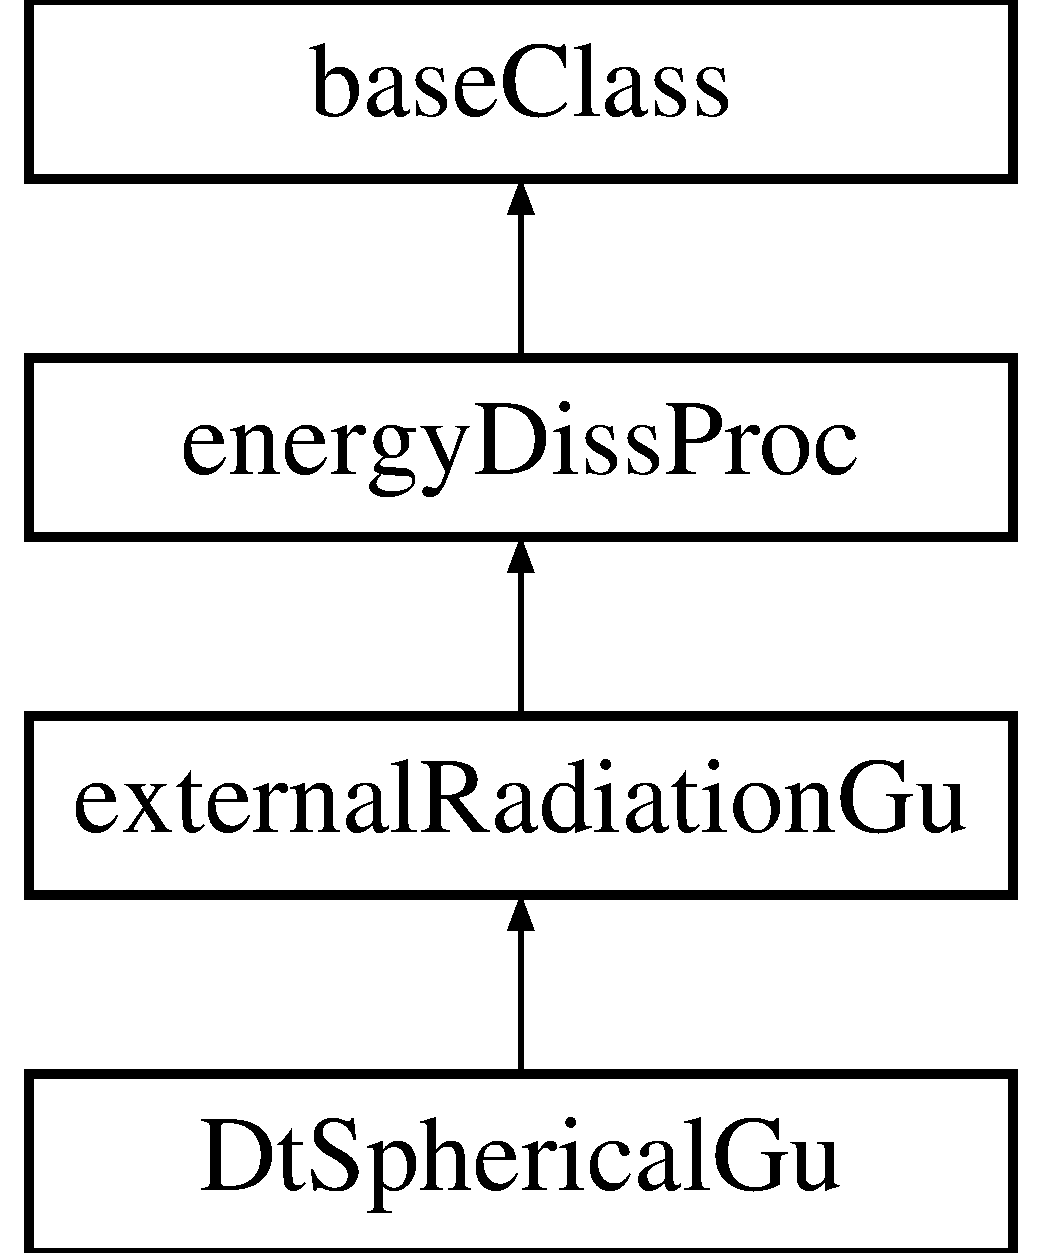
\includegraphics[height=4.000000cm]{classDtSphericalGu}
\end{center}
\end{figure}


\subsection{Detailed Description}
Parameters used by class (defaults) 
\begin{DoxyParams}{Parameters}
{\em e} & (\hyperlink{classexternalRadiationGu}{external\-Radiation\-Gu}) -\/ energy (ext) in e\-V (e = 0.\-6203) \\
\hline
{\em cf} & (external\-Radiation\-Spherical\-Gu) -\/ covering factor (cf = 0.\-1) \\
\hline
{\em rext} & -\/ blr radius (rext = 1.\-0$\ast$r\-\_\-sub) \\
\hline
{\em k} & -\/ u\-\_\-ext vs r index = 2 \\
\hline
\end{DoxyParams}
\subsection*{Public Member Functions}
\begin{DoxyCompactItemize}
\item 
\hyperlink{classDtSphericalGu_ac10430f174e0e5c62da42b2bdae446d3}{Dt\-Spherical\-Gu} (scfgp $\ast$\-\_\-cfg, \hyperlink{classjetGeometry}{jet\-Geometry} $\ast$\-\_\-r, \hyperlink{classelectrons}{electrons} $\ast$\-\_\-ele, std\-::string \-\_\-id)
\item 
\hyperlink{classDtSphericalGu_a6f5f80e9ef2f5f15283cec5ab074a1bb}{$\sim$\-Dt\-Spherical\-Gu} ()
\item 
void \hyperlink{classDtSphericalGu_aeed0bda6440570b686aaf85bf5d2b6b3}{print\-Info} ()
\item 
void \hyperlink{classDtSphericalGu_ac940befec9ea9886b136f9d96c88620a}{update} ()
\item 
double \hyperlink{classDtSphericalGu_a78218d880e1c9374058b6084ca939804}{getvext} (double \-\_\-r)
\item 
void \hyperlink{classDtSphericalGu_af8b00665c5f7caca8b4a84034a097e05}{set\-Radius} ()
\end{DoxyCompactItemize}
\subsection*{Additional Inherited Members}


\subsection{Constructor \& Destructor Documentation}
\hypertarget{classDtSphericalGu_ac10430f174e0e5c62da42b2bdae446d3}{\index{Dt\-Spherical\-Gu@{Dt\-Spherical\-Gu}!Dt\-Spherical\-Gu@{Dt\-Spherical\-Gu}}
\index{Dt\-Spherical\-Gu@{Dt\-Spherical\-Gu}!DtSphericalGu@{Dt\-Spherical\-Gu}}
\subsubsection[{Dt\-Spherical\-Gu}]{\setlength{\rightskip}{0pt plus 5cm}Dt\-Spherical\-Gu\-::\-Dt\-Spherical\-Gu (
\begin{DoxyParamCaption}
\item[{scfgp $\ast$}]{\-\_\-cfg, }
\item[{{\bf jet\-Geometry} $\ast$}]{\-\_\-r, }
\item[{{\bf electrons} $\ast$}]{\-\_\-ele, }
\item[{std\-::string}]{\-\_\-id}
\end{DoxyParamCaption}
)}}\label{classDtSphericalGu_ac10430f174e0e5c62da42b2bdae446d3}
constructor 
\begin{DoxyParams}{Parameters}
{\em \-\_\-cfg} & -\/ scfgp class object \\
\hline
{\em \-\_\-r} & -\/ \hyperlink{classjetGeometry}{jet\-Geometry} class object \\
\hline
{\em \-\_\-ele} & -\/ electrons class object \\
\hline
{\em \-\_\-id} & \\
\hline
\end{DoxyParams}

\begin{DoxyCode}
9                                                                                        : 
      \hyperlink{classexternalRadiationGu_aad5903b642f08594be10d699cf9fb3b4}{externalRadiationGu}( \hyperlink{classbaseClass_a744f87a6ebe63da08256c022d42a4ca7}{cfg}, \hyperlink{classbaseClass_a482bb9b1d94f3eb3f31026d14e9a2bb6}{r}, \hyperlink{classenergyDissProc_a0dbf0777938131e938c1fdad5df38a7f}{ele}, \textcolor{keywordtype}{id} ) \{
10   \textcolor{comment}{/* requested parameters */}
11   \hyperlink{classbaseClass_a744f87a6ebe63da08256c022d42a4ca7}{cfg} -> request<double>(\textcolor{keywordtype}{id} + \textcolor{stringliteral}{"e"}, 0.6203, &e );
12   \hyperlink{classbaseClass_a744f87a6ebe63da08256c022d42a4ca7}{cfg} -> request<double>(\textcolor{keywordtype}{id} + \textcolor{stringliteral}{"cf"}, 0.1, &cf );
13   \hyperlink{classbaseClass_a744f87a6ebe63da08256c022d42a4ca7}{cfg} -> request<double>(\textcolor{keywordtype}{id} + \textcolor{stringliteral}{"rext"}, 0.0, &rext );
14   \hyperlink{classbaseClass_a744f87a6ebe63da08256c022d42a4ca7}{cfg} -> request<double>(\textcolor{keywordtype}{id} + \textcolor{stringliteral}{"k"}, 2.0, &k );
15 
16   \hyperlink{classbaseClass_a744f87a6ebe63da08256c022d42a4ca7}{cfg} -> updateRequests( );
17 
18   \textcolor{keywordflow}{if}( rext == 0.0 ) \{ \hyperlink{classDtSphericalGu_af8b00665c5f7caca8b4a84034a097e05}{setRadius}( ); \}
19   \textcolor{keywordflow}{else} \{ bazinga::warning(\textcolor{keywordtype}{id},\textcolor{stringliteral}{"Overwritting rext value from config file!"}); \}
20   
21   \hyperlink{classenergyDissProc_aafedd3c012010a8e8aa34247660fea3b}{vpMin} = 0.01*DSQR( \hyperlink{classenergyDissProc_a0dbf0777938131e938c1fdad5df38a7f}{ele} -> getGammaMin( ) )*\hyperlink{classDtSphericalGu_a78218d880e1c9374058b6084ca939804}{getvext}( \hyperlink{classbaseClass_a482bb9b1d94f3eb3f31026d14e9a2bb6}{r}->getRMax() );
22   vpMax = 100.0*DSQR( \hyperlink{classenergyDissProc_a0dbf0777938131e938c1fdad5df38a7f}{ele} -> getGammaMax( ) )*\hyperlink{classDtSphericalGu_a78218d880e1c9374058b6084ca939804}{getvext}( \hyperlink{classbaseClass_a482bb9b1d94f3eb3f31026d14e9a2bb6}{r}->getR0() );
23 
24   allocateUpeR( ); \textcolor{comment}{// this is for storing vector information about Upe(r) }
25   allocateLpv( );
26   allocateLvPoint( );
27   allocateLvPointAvg( );
28 
29   \textcolor{keywordflow}{for}( \textcolor{keywordtype}{int} i=0;i<\hyperlink{classbaseClass_a2b4d07d2b46197d495de0477f4bb22f8}{N};i++ ) \{ set\_vp( i, \hyperlink{classenergyDissProc_aafedd3c012010a8e8aa34247660fea3b}{vpMin}*pow( vpMax/\hyperlink{classenergyDissProc_aafedd3c012010a8e8aa34247660fea3b}{vpMin},(\textcolor{keywordtype}{double})i/((\textcolor{keywordtype}{double})N-1)) ); \}
30 \}
\end{DoxyCode}
\hypertarget{classDtSphericalGu_a6f5f80e9ef2f5f15283cec5ab074a1bb}{\index{Dt\-Spherical\-Gu@{Dt\-Spherical\-Gu}!$\sim$\-Dt\-Spherical\-Gu@{$\sim$\-Dt\-Spherical\-Gu}}
\index{$\sim$\-Dt\-Spherical\-Gu@{$\sim$\-Dt\-Spherical\-Gu}!DtSphericalGu@{Dt\-Spherical\-Gu}}
\subsubsection[{$\sim$\-Dt\-Spherical\-Gu}]{\setlength{\rightskip}{0pt plus 5cm}Dt\-Spherical\-Gu\-::$\sim$\-Dt\-Spherical\-Gu (
\begin{DoxyParamCaption}
{}
\end{DoxyParamCaption}
)\hspace{0.3cm}{\ttfamily [inline]}}}\label{classDtSphericalGu_a6f5f80e9ef2f5f15283cec5ab074a1bb}
destructor 
\begin{DoxyCode}
35 \{ \}
\end{DoxyCode}


\subsection{Member Function Documentation}
\hypertarget{classDtSphericalGu_a78218d880e1c9374058b6084ca939804}{\index{Dt\-Spherical\-Gu@{Dt\-Spherical\-Gu}!getvext@{getvext}}
\index{getvext@{getvext}!DtSphericalGu@{Dt\-Spherical\-Gu}}
\subsubsection[{getvext}]{\setlength{\rightskip}{0pt plus 5cm}double Dt\-Spherical\-Gu\-::getvext (
\begin{DoxyParamCaption}
\item[{double}]{\-\_\-r}
\end{DoxyParamCaption}
)\hspace{0.3cm}{\ttfamily [virtual]}}}\label{classDtSphericalGu_a78218d880e1c9374058b6084ca939804}
get v\-\_\-ext value in Hz 
\begin{DoxyParams}{Parameters}
{\em \-\_\-r} & -\/ radius \\
\hline
\end{DoxyParams}
\begin{DoxyReturn}{Returns}
v\-\_\-ext 
\end{DoxyReturn}


Reimplemented from \hyperlink{classexternalRadiationGu_ab7e1abcc40cf0538404e88a0febdfb02}{external\-Radiation\-Gu}.


\begin{DoxyCode}
32                                          \{
33   \textcolor{keywordtype}{double} vext;
34   vext = e*eV2erg/PLANCK\_H;
35   \textcolor{keywordflow}{if}( \hyperlink{classenergyDissProc_a0a23854c1c830dfb9ac33d116fce5b7d}{luminosityConstNu} ) \{ \textcolor{keywordflow}{return} vext; \}
36   \textcolor{keywordflow}{else} \{ \textcolor{keywordflow}{return} vext*rext/\_r; \}
37 \}
\end{DoxyCode}
\hypertarget{classDtSphericalGu_aeed0bda6440570b686aaf85bf5d2b6b3}{\index{Dt\-Spherical\-Gu@{Dt\-Spherical\-Gu}!print\-Info@{print\-Info}}
\index{print\-Info@{print\-Info}!DtSphericalGu@{Dt\-Spherical\-Gu}}
\subsubsection[{print\-Info}]{\setlength{\rightskip}{0pt plus 5cm}void Dt\-Spherical\-Gu\-::print\-Info (
\begin{DoxyParamCaption}
{}
\end{DoxyParamCaption}
)\hspace{0.3cm}{\ttfamily [virtual]}}}\label{classDtSphericalGu_aeed0bda6440570b686aaf85bf5d2b6b3}
print basic information about myself (virtual) 

Reimplemented from \hyperlink{classexternalRadiationGu_a8aa28d939b0ecf2651f18cc4f5f6ba25}{external\-Radiation\-Gu}.


\begin{DoxyCode}
52                                \{
53   bazinga::info(\textcolor{keywordtype}{id},\textcolor{stringliteral}{"Info"});
54   bazinga::print\_info(\textcolor{keywordtype}{id},\textcolor{stringliteral}{"N"},\hyperlink{classbaseClass_a2b4d07d2b46197d495de0477f4bb22f8}{N});
55   bazinga::print\_info(\textcolor{keywordtype}{id},\textcolor{stringliteral}{"Avg energy (in external frame)"},e,\textcolor{stringliteral}{"eV"});
56   bazinga::print\_info(\textcolor{keywordtype}{id},\textcolor{stringliteral}{"Avg frequency (in external frame)"},\hyperlink{classDtSphericalGu_a78218d880e1c9374058b6084ca939804}{getvext}( \hyperlink{classbaseClass_a482bb9b1d94f3eb3f31026d14e9a2bb6}{r}->getR0()),\textcolor{stringliteral}{"Hz"});
57   bazinga::print\_info(\textcolor{keywordtype}{id},\textcolor{stringliteral}{"Clouds covering factor cf"},cf);
58   bazinga::print\_info(\textcolor{keywordtype}{id},\textcolor{stringliteral}{"radius rext"},rext,\textcolor{stringliteral}{"cm"});
59   bazinga::print\_info(\textcolor{keywordtype}{id},\textcolor{stringliteral}{"strat index k"},k);
60   bazinga::print\_info(\textcolor{keywordtype}{id},\textcolor{stringliteral}{"vpMin"},\hyperlink{classenergyDissProc_aafedd3c012010a8e8aa34247660fea3b}{vpMin},\textcolor{stringliteral}{"Hz"});
61   bazinga::print\_info(\textcolor{keywordtype}{id},\textcolor{stringliteral}{"vpMax"},vpMax,\textcolor{stringliteral}{"Hz"});
62 \}
\end{DoxyCode}
\hypertarget{classDtSphericalGu_af8b00665c5f7caca8b4a84034a097e05}{\index{Dt\-Spherical\-Gu@{Dt\-Spherical\-Gu}!set\-Radius@{set\-Radius}}
\index{set\-Radius@{set\-Radius}!DtSphericalGu@{Dt\-Spherical\-Gu}}
\subsubsection[{set\-Radius}]{\setlength{\rightskip}{0pt plus 5cm}void Dt\-Spherical\-Gu\-::set\-Radius (
\begin{DoxyParamCaption}
{}
\end{DoxyParamCaption}
)\hspace{0.3cm}{\ttfamily [virtual]}}}\label{classDtSphericalGu_af8b00665c5f7caca8b4a84034a097e05}
sets rext if not provided by config file 

Reimplemented from \hyperlink{classexternalRadiationGu_a541b2bb7da733f10d83af6225b7ad5f8}{external\-Radiation\-Gu}.


\begin{DoxyCode}
64                                 \{
65   \textcolor{keywordtype}{double} Ledd = 1.3e47*mBH;
66   \textcolor{keywordtype}{double} Ldisk = eDisk*mDot*Ledd;
67   \textcolor{keywordtype}{double} R\_sub = 1.6e-5*sqrt( Ldisk );
68   rext = R\_sub; \}
\end{DoxyCode}
\hypertarget{classDtSphericalGu_ac940befec9ea9886b136f9d96c88620a}{\index{Dt\-Spherical\-Gu@{Dt\-Spherical\-Gu}!update@{update}}
\index{update@{update}!DtSphericalGu@{Dt\-Spherical\-Gu}}
\subsubsection[{update}]{\setlength{\rightskip}{0pt plus 5cm}void Dt\-Spherical\-Gu\-::update (
\begin{DoxyParamCaption}
{}
\end{DoxyParamCaption}
)\hspace{0.3cm}{\ttfamily [virtual]}}}\label{classDtSphericalGu_ac940befec9ea9886b136f9d96c88620a}
calculate and set Upe every time with new radius r 

Reimplemented from \hyperlink{classexternalRadiationGu_a730363f393f29aef9927e0bb84087116}{external\-Radiation\-Gu}.


\begin{DoxyCode}
39                              \{
40   \textcolor{keywordtype}{double} Ledd = 1.3e47*mBH;
41   \textcolor{keywordtype}{double} Ldisk = eDisk*mDot*Ledd;
42   \textcolor{keywordtype}{double} temp\_upe = 0.0;
43   \textcolor{keywordtype}{double} temp\_cf = 0.0;
44   temp\_cf = cf;
45   temp\_cf *= pow(\hyperlink{classbaseClass_a482bb9b1d94f3eb3f31026d14e9a2bb6}{r}->get()/rext,2)/(1.0+pow(\hyperlink{classbaseClass_a482bb9b1d94f3eb3f31026d14e9a2bb6}{r}->get()/rext,k));
46   temp\_upe = (temp\_cf*Ldisk*DSQR(Gamma))/(3.0*M\_PI*DSQR(\hyperlink{classbaseClass_a482bb9b1d94f3eb3f31026d14e9a2bb6}{r}->get())*LIGHT\_SPEED);
47   gsl\_vector\_set( \hyperlink{classenergyDissProc_ac925d66519c79f36421f75a6bc9f0965}{upe\_r}, \hyperlink{classbaseClass_a482bb9b1d94f3eb3f31026d14e9a2bb6}{r}->getIndex( ), temp\_upe );
48   bazinga::print\_info(\textcolor{keywordtype}{id},\textcolor{stringliteral}{"Upe"},gsl\_vector\_get( \hyperlink{classenergyDissProc_ac925d66519c79f36421f75a6bc9f0965}{upe\_r}, \hyperlink{classbaseClass_a482bb9b1d94f3eb3f31026d14e9a2bb6}{r}->getIndex( ) ) );
49   set\_upe\_r( gsl\_vector\_get( \hyperlink{classenergyDissProc_ac925d66519c79f36421f75a6bc9f0965}{upe\_r}, \hyperlink{classbaseClass_a482bb9b1d94f3eb3f31026d14e9a2bb6}{r}->getIndex( ) ) );
50   \hyperlink{classenergyDissProc_a7b51925f603e271657cab66afe822591}{flag\_upe\_r} = \textcolor{keyword}{false}; \}
\end{DoxyCode}


The documentation for this class was generated from the following files\-:\begin{DoxyCompactItemize}
\item 
/home/mjaniak/\-Soft/blazar++/include/\hyperlink{DtSphericalGu_8hpp}{Dt\-Spherical\-Gu.\-hpp}\item 
/home/mjaniak/\-Soft/blazar++/src/\hyperlink{DtSphericalGu_8cpp}{Dt\-Spherical\-Gu.\-cpp}\end{DoxyCompactItemize}

\hypertarget{classelectrons}{\section{electrons Class Reference}
\label{classelectrons}\index{electrons@{electrons}}
}


{\ttfamily \#include $<$electrons.\-hpp$>$}

Inheritance diagram for electrons\-:\begin{figure}[H]
\begin{center}
\leavevmode
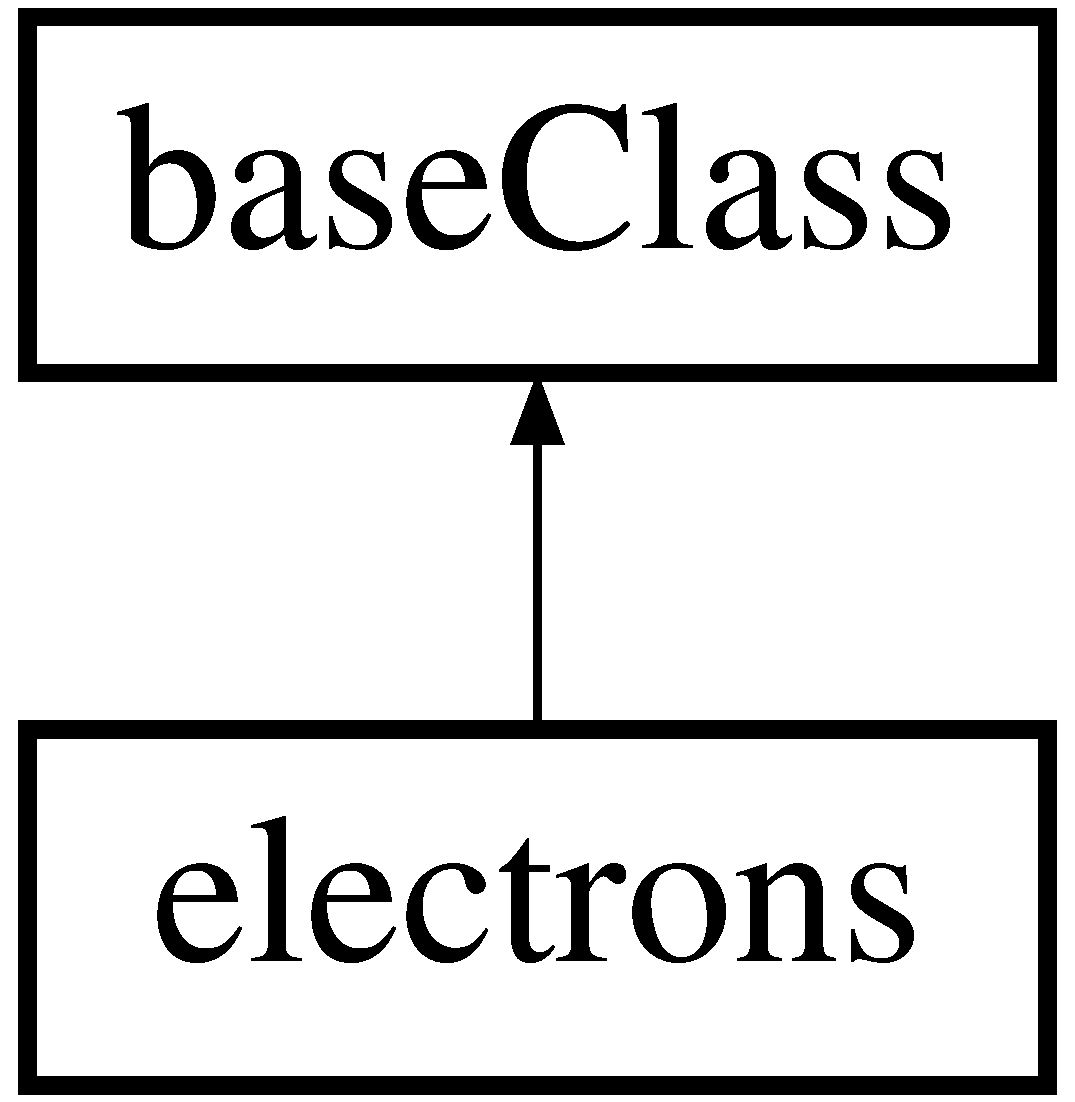
\includegraphics[height=2.000000cm]{classelectrons}
\end{center}
\end{figure}


\subsection{Detailed Description}
Class to hold all detaild for electrons in the jet (all calculated in jet co-\/moving frame); it is responsible for calculating energy losses, solving propagation equation, electron energy spectrum etc. \subsection*{Public Member Functions}
\begin{DoxyCompactItemize}
\item 
\hyperlink{classelectrons_a5532b5fbcb8b735e50116227aa8f2ebc}{electrons} (scfgp $\ast$\-\_\-cfg, \hyperlink{classjetGeometry}{jet\-Geometry} $\ast$\-\_\-r, std\-::string \-\_\-id)
\item 
\hyperlink{classelectrons_a146d787f88697a2ca2acaa245055d63b}{$\sim$electrons} ()
\item 
double \hyperlink{classelectrons_aefdd16f24a2f35cef7f5d01930da00ee}{t\-Q} (double g, double \-\_\-radius)
\item 
double \hyperlink{classelectrons_aa47f9474892a92a011f952731bf1cdeb}{gauss} (double \-\_\-radius)
\item 
double \hyperlink{classelectrons_aa9fa0208f23e0a28f50652606a7f7481}{gaussmod} (double \-\_\-radius)
\item 
double \hyperlink{classelectrons_a75b123e6b9d2ff587bee4a4be4fa3bbe}{tri} (double \-\_\-radius)
\item 
double \hyperlink{classelectrons_ae87edc2ea2e2ce2050fa554da90f2852}{inject} ()
\item 
void \hyperlink{classelectrons_a4e45b3bf040e39dad560d3b7e6572c90}{evolve} ()
\item 
double \hyperlink{classelectrons_afe0e0014e58c500a9bcf62357f781263}{dgdr} (double g)
\item 
double \hyperlink{classelectrons_afb0d9365f13787f44d23fb489732fc90}{get\-Gamma} (int i)
\item 
double \hyperlink{classelectrons_a24fbbed0acac968ce6b2ef2c5043dee4}{get\-Ngamma} (int i)
\item 
void \hyperlink{classelectrons_a41db9252c408dd206342f0d23c8edb96}{add\-En\-Diss\-Proc} (\hyperlink{classenergyDissProc}{energy\-Diss\-Proc} $\ast$\-\_\-obj)
\item 
void \hyperlink{classelectrons_a771ec6a114df4f41d09273f1c57db07d}{list\-En\-Diss\-Proc} ()
\item 
void \hyperlink{classelectrons_ace657f207a4f68058b2606ff2772f3c5}{print\-Info} ()
\item 
void \hyperlink{classelectrons_a6e630bdecdc411683d02bbcf8aa82a56}{print\-Cooling\-Info} (double g)
\item 
void \hyperlink{classelectrons_af5e619dff4d9716328664a9625b6e8dd}{avg\-Ngamma} ()
\item 
void \hyperlink{classelectrons_ad94a7b6cc694ef0e70f7efaadef8463d}{set\-Injection\-Parameters} ()
\item 
void \hyperlink{classelectrons_aac9514f742569f37097d13b3ea04239a}{set\-Energetics} ()
\item 
\hypertarget{classelectrons_ad94d84888078393333deedf0fbdad3dd}{double {\bfseries get\-Gamma\-Min} ()}\label{classelectrons_ad94d84888078393333deedf0fbdad3dd}

\item 
\hypertarget{classelectrons_aa5dfd8ba29a4bc1b7de5bf7bf64d69e3}{double {\bfseries get\-Gamma\-Max} ()}\label{classelectrons_aa5dfd8ba29a4bc1b7de5bf7bf64d69e3}

\item 
double \hyperlink{classelectrons_a22aacb80ac20a46f471430db72c95b71}{beta} (double x)
\item 
double \hyperlink{classelectrons_a4e3d4179ce211bd732580b49914874e6}{getd\-Log\-Gamma} ()
\item 
int \hyperlink{classelectrons_a18a3cd4a19f833931632da1f9800141f}{if\-Evol} ()
\item 
void \hyperlink{classelectrons_ab509cb088f16247eec3a15b9c35bc23e}{save\-Injection} ()
\item 
void \hyperlink{classelectrons_ae1bc246f7783a9b65bd1f1678bfe5cd2}{save\-Ngamma} ()
\item 
void \hyperlink{classelectrons_aac83390f974136b1bc365b36ef460723}{save\-Ngamma\-Avg} ()
\end{DoxyCompactItemize}
\subsection*{Public Attributes}
\begin{DoxyCompactItemize}
\item 
std\-::vector$<$ \hyperlink{classenergyDissProc}{energy\-Diss\-Proc} $\ast$ $>$ \hyperlink{classelectrons_a2c90bebdf0a961a720dc9b70306fb6ea}{En\-Diss\-Proc}
\item 
gsl\-\_\-vector $\ast$ \hyperlink{classelectrons_aba72b6575be27358efcb13cc3415df68}{gamma}
\item 
\hypertarget{classelectrons_ac2a11c35da2adfdf2f9ad915be55ca33}{gsl\-\_\-vector $\ast$ {\bfseries Ngamma}}\label{classelectrons_ac2a11c35da2adfdf2f9ad915be55ca33}

\item 
\hypertarget{classelectrons_aaea12887510456458b7a318edf62d4f0}{gsl\-\_\-vector $\ast$ {\bfseries Ngamma\-Avg}}\label{classelectrons_aaea12887510456458b7a318edf62d4f0}

\item 
gsl\-\_\-vector $\ast$ \hyperlink{classelectrons_a5d1c72cf1ee40f0e918fbb2d9d13393b}{A}
\item 
\hypertarget{classelectrons_a7ec0598cb033a2e77c2af1c5ef852658}{gsl\-\_\-vector $\ast$ {\bfseries B}}\label{classelectrons_a7ec0598cb033a2e77c2af1c5ef852658}

\item 
\hypertarget{classelectrons_ace04a2cb2a5ce764d53bb4a99461e709}{gsl\-\_\-vector $\ast$ {\bfseries C}}\label{classelectrons_ace04a2cb2a5ce764d53bb4a99461e709}

\item 
\hypertarget{classelectrons_ade5ba73efe54cddda0550d8de323e91d}{gsl\-\_\-vector $\ast$ {\bfseries S}}\label{classelectrons_ade5ba73efe54cddda0550d8de323e91d}

\item 
\hypertarget{classelectrons_afcef79a408b1a8f956573b85de8fb4ba}{gsl\-\_\-vector $\ast$ {\bfseries U}}\label{classelectrons_afcef79a408b1a8f956573b85de8fb4ba}

\end{DoxyCompactItemize}


\subsection{Constructor \& Destructor Documentation}
\hypertarget{classelectrons_a5532b5fbcb8b735e50116227aa8f2ebc}{\index{electrons@{electrons}!electrons@{electrons}}
\index{electrons@{electrons}!electrons@{electrons}}
\subsubsection[{electrons}]{\setlength{\rightskip}{0pt plus 5cm}electrons\-::electrons (
\begin{DoxyParamCaption}
\item[{scfgp $\ast$}]{\-\_\-cfg, }
\item[{{\bf jet\-Geometry} $\ast$}]{\-\_\-r, }
\item[{std\-::string}]{\-\_\-id}
\end{DoxyParamCaption}
)}}\label{classelectrons_a5532b5fbcb8b735e50116227aa8f2ebc}
constructor 
\begin{DoxyParams}{Parameters}
{\em scfgp} & \\
\hline
{\em \hyperlink{classjetGeometry}{jet\-Geometry}} & \\
\hline
{\em id} & \\
\hline
\end{DoxyParams}

\begin{DoxyCode}
10                                                                   : \hyperlink{classbaseClass}{baseClass}(\_cfg, \_r, \_id ) \{
11   \textcolor{comment}{/* requested parameters */}
12   \hyperlink{classbaseClass_a744f87a6ebe63da08256c022d42a4ca7}{cfg} -> request<int>(\textcolor{stringliteral}{"N"}+\hyperlink{classbaseClass_a4d5ff386a69bcbe21b5976f55b624df6}{id},200,&\hyperlink{classbaseClass_a2b4d07d2b46197d495de0477f4bb22f8}{N});
13   \hyperlink{classbaseClass_a744f87a6ebe63da08256c022d42a4ca7}{cfg} -> request<std::string>(\textcolor{stringliteral}{"eleModel"},\textcolor{stringliteral}{"blob"},&eleModel);
14   \hyperlink{classbaseClass_a744f87a6ebe63da08256c022d42a4ca7}{cfg} -> request<std::string>(\textcolor{stringliteral}{"injModel"},\textcolor{stringliteral}{"REC"},&injModel);
15   \hyperlink{classbaseClass_a744f87a6ebe63da08256c022d42a4ca7}{cfg} -> request<std::string>(\textcolor{stringliteral}{"lumModel"},\textcolor{stringliteral}{"blob"},&lumModel);
16   \hyperlink{classbaseClass_a744f87a6ebe63da08256c022d42a4ca7}{cfg} -> request<double>(\textcolor{stringliteral}{"p1"},2.0,&p1);
17   \hyperlink{classbaseClass_a744f87a6ebe63da08256c022d42a4ca7}{cfg} -> request<double>(\textcolor{stringliteral}{"p2"},2.0,&p2);
18   \hyperlink{classbaseClass_a744f87a6ebe63da08256c022d42a4ca7}{cfg} -> request<double>(\textcolor{stringliteral}{"gammaMin"},1.0,&gammaMin);
19   \hyperlink{classbaseClass_a744f87a6ebe63da08256c022d42a4ca7}{cfg} -> request<double>(\textcolor{stringliteral}{"gammaBreak"},0.0,&gammaBreak);
20   \hyperlink{classbaseClass_a744f87a6ebe63da08256c022d42a4ca7}{cfg} -> request<double>(\textcolor{stringliteral}{"gammaMax"},1.0e2,&gammaMax);
21   \hyperlink{classbaseClass_a744f87a6ebe63da08256c022d42a4ca7}{cfg} -> request<double>(\textcolor{stringliteral}{"injRm"},2.0e17,&injRm);
22   \hyperlink{classbaseClass_a744f87a6ebe63da08256c022d42a4ca7}{cfg} -> request<double>(\textcolor{stringliteral}{"injSigma"},0.6,&injSigma);
23   \hyperlink{classbaseClass_a744f87a6ebe63da08256c022d42a4ca7}{cfg} -> request<double>(\textcolor{stringliteral}{"eleK"},0.0,&eleK);
24   \hyperlink{classbaseClass_a744f87a6ebe63da08256c022d42a4ca7}{cfg} -> request<double>(\textcolor{stringliteral}{"eEle"},0.1,&eEle);
25   \hyperlink{classbaseClass_a744f87a6ebe63da08256c022d42a4ca7}{cfg} -> request<double>(\textcolor{stringliteral}{"eDiss"},0.1,&eDiss);
26   \hyperlink{classbaseClass_a744f87a6ebe63da08256c022d42a4ca7}{cfg} -> request<double>(\textcolor{stringliteral}{"Gamma"},10.0,&Gamma);
27   \hyperlink{classbaseClass_a744f87a6ebe63da08256c022d42a4ca7}{cfg} -> request<double>(\textcolor{stringliteral}{"NeNp"},0.1,&NeNp);
28   \hyperlink{classbaseClass_a744f87a6ebe63da08256c022d42a4ca7}{cfg} -> request<double>(\textcolor{stringliteral}{"mBH"},1.0,&mBH);
29   \hyperlink{classbaseClass_a744f87a6ebe63da08256c022d42a4ca7}{cfg} -> request<double>(\textcolor{stringliteral}{"eDisk"},0.1,&eDisk);
30   \hyperlink{classbaseClass_a744f87a6ebe63da08256c022d42a4ca7}{cfg} -> request<double>(\textcolor{stringliteral}{"mDot"},1.0,&mDot);
31   \hyperlink{classbaseClass_a744f87a6ebe63da08256c022d42a4ca7}{cfg} -> request<double>(\textcolor{stringliteral}{"eJet"},0.3,&eJet);
32   \hyperlink{classbaseClass_a744f87a6ebe63da08256c022d42a4ca7}{cfg} -> request<double>(\textcolor{stringliteral}{"sigmaB"},0.1,&sigmaB);
33   \hyperlink{classbaseClass_a744f87a6ebe63da08256c022d42a4ca7}{cfg} -> request<int>(\textcolor{stringliteral}{"evol"},0,&evol);
34   \hyperlink{classbaseClass_a744f87a6ebe63da08256c022d42a4ca7}{cfg} -> request<int>(\textcolor{stringliteral}{"saveElectrons"},1,&saveElectrons);
35   \hyperlink{classbaseClass_a744f87a6ebe63da08256c022d42a4ca7}{cfg} -> request<int>(\textcolor{stringliteral}{"saveElectronsAvg"},1,&saveElectronsAvg);
36 
37   \hyperlink{classbaseClass_a744f87a6ebe63da08256c022d42a4ca7}{cfg} -> updateRequests( );
38 
39   \textcolor{comment}{/* check if spectral indices are OK; for steady model p1 must be lower than 1 and p2 must be greater than
       2; otherwise calculation of break electron energy will fail;}
40 \textcolor{comment}{     for blob model it is all good to set any indices you like */}
41   \textcolor{keywordflow}{if}( (p1 > 1.0 || p2 < 2.0) && eleModel == \textcolor{stringliteral}{"steady"} && gammaBreak == 0.0 ) \{
42     bazinga::warning(\textcolor{keywordtype}{id},\textcolor{stringliteral}{"Can't use steady model with p1>1.0 or p2<2.0!"});
43     bazinga::warning(\textcolor{keywordtype}{id},\textcolor{stringliteral}{"To overwrite that you can set gammaBreak explicity."});
44     bazinga::warning(\textcolor{keywordtype}{id},\textcolor{stringliteral}{"Quit."});
45     exit(0); \}
46 
47   allocateGamma( );
48   allocateTridiag( );
49   
50   \textcolor{keywordflow}{for}( \textcolor{keywordtype}{int} i=0;i<=\hyperlink{classbaseClass_a2b4d07d2b46197d495de0477f4bb22f8}{N}+1;i++ ) \{ gsl\_vector\_set( \hyperlink{classelectrons_aba72b6575be27358efcb13cc3415df68}{gamma}, i, pow( gammaMax,(\textcolor{keywordtype}{double})i/(\textcolor{keywordtype}{double})
      \hyperlink{classbaseClass_a2b4d07d2b46197d495de0477f4bb22f8}{N} )); \}
51 
52   \hyperlink{classelectrons_aac9514f742569f37097d13b3ea04239a}{setEnergetics}( );
53   \hyperlink{classelectrons_ad94a7b6cc694ef0e70f7efaadef8463d}{setInjectionParameters}( );
54   dLogGamma = log( gsl\_vector\_get(\hyperlink{classelectrons_aba72b6575be27358efcb13cc3415df68}{gamma},1)/gsl\_vector\_get(\hyperlink{classelectrons_aba72b6575be27358efcb13cc3415df68}{gamma},0) ); \}
\end{DoxyCode}
\hypertarget{classelectrons_a146d787f88697a2ca2acaa245055d63b}{\index{electrons@{electrons}!$\sim$electrons@{$\sim$electrons}}
\index{$\sim$electrons@{$\sim$electrons}!electrons@{electrons}}
\subsubsection[{$\sim$electrons}]{\setlength{\rightskip}{0pt plus 5cm}electrons\-::$\sim$electrons (
\begin{DoxyParamCaption}
{}
\end{DoxyParamCaption}
)}}\label{classelectrons_a146d787f88697a2ca2acaa245055d63b}
destructor 
\begin{DoxyCode}
140                        \{
141   freeGamma( );
142   freeTridiag( ); \}
\end{DoxyCode}


\subsection{Member Function Documentation}
\hypertarget{classelectrons_a41db9252c408dd206342f0d23c8edb96}{\index{electrons@{electrons}!add\-En\-Diss\-Proc@{add\-En\-Diss\-Proc}}
\index{add\-En\-Diss\-Proc@{add\-En\-Diss\-Proc}!electrons@{electrons}}
\subsubsection[{add\-En\-Diss\-Proc}]{\setlength{\rightskip}{0pt plus 5cm}void electrons\-::add\-En\-Diss\-Proc (
\begin{DoxyParamCaption}
\item[{{\bf energy\-Diss\-Proc} $\ast$}]{\-\_\-obj}
\end{DoxyParamCaption}
)}}\label{classelectrons_a41db9252c408dd206342f0d23c8edb96}
add process to energy dissipation 
\begin{DoxyParams}{Parameters}
{\em \hyperlink{classenergyDissProc}{energy\-Diss\-Proc}} & \\
\hline
\end{DoxyParams}

\begin{DoxyCode}
234 \{ \hyperlink{classelectrons_a2c90bebdf0a961a720dc9b70306fb6ea}{EnDissProc}.push\_back( \_obj ); \}
\end{DoxyCode}
\hypertarget{classelectrons_af5e619dff4d9716328664a9625b6e8dd}{\index{electrons@{electrons}!avg\-Ngamma@{avg\-Ngamma}}
\index{avg\-Ngamma@{avg\-Ngamma}!electrons@{electrons}}
\subsubsection[{avg\-Ngamma}]{\setlength{\rightskip}{0pt plus 5cm}void electrons\-::avg\-Ngamma (
\begin{DoxyParamCaption}
{}
\end{DoxyParamCaption}
)}}\label{classelectrons_af5e619dff4d9716328664a9625b6e8dd}
calculate averaged electron distribution 
\begin{DoxyCode}
361                            \{
362   \textcolor{keywordflow}{for}( \textcolor{keywordtype}{int} i=0;i<\hyperlink{classbaseClass_a2b4d07d2b46197d495de0477f4bb22f8}{N};i++ ) \{ gsl\_vector\_set( NgammaAvg, i, gsl\_vector\_get( NgammaAvg, i ) + 
      \hyperlink{classelectrons_a24fbbed0acac968ce6b2ef2c5043dee4}{getNgamma}( i ) ); \} 
363 \}
\end{DoxyCode}
\hypertarget{classelectrons_a22aacb80ac20a46f471430db72c95b71}{\index{electrons@{electrons}!beta@{beta}}
\index{beta@{beta}!electrons@{electrons}}
\subsubsection[{beta}]{\setlength{\rightskip}{0pt plus 5cm}double electrons\-::beta (
\begin{DoxyParamCaption}
\item[{double}]{x}
\end{DoxyParamCaption}
)}}\label{classelectrons_a22aacb80ac20a46f471430db72c95b71}
probably doubled from \hyperlink{classbaseClass}{base\-Class}?? 
\begin{DoxyCode}
373 \{ \textcolor{keywordflow}{return} sqrt(1.0-1.0/(x*x)); \}
\end{DoxyCode}
\hypertarget{classelectrons_afe0e0014e58c500a9bcf62357f781263}{\index{electrons@{electrons}!dgdr@{dgdr}}
\index{dgdr@{dgdr}!electrons@{electrons}}
\subsubsection[{dgdr}]{\setlength{\rightskip}{0pt plus 5cm}double electrons\-::dgdr (
\begin{DoxyParamCaption}
\item[{double}]{g}
\end{DoxyParamCaption}
)}}\label{classelectrons_afe0e0014e58c500a9bcf62357f781263}
get electron cooling details 
\begin{DoxyParams}{Parameters}
{\em g} & -\/ electron Lorentz factor \\
\hline
\end{DoxyParams}
\begin{DoxyReturn}{Returns}
d gamma \textbackslash{} d t 
\end{DoxyReturn}

\begin{DoxyCode}
222                                  \{
223   \textcolor{keywordtype}{double} dotg = 0.0;
224   \textcolor{keywordflow}{for}( \textcolor{keywordtype}{int} i=0; i<\hyperlink{classelectrons_a2c90bebdf0a961a720dc9b70306fb6ea}{EnDissProc}.size(); i++ ) \{ dotg += \hyperlink{classelectrons_a2c90bebdf0a961a720dc9b70306fb6ea}{EnDissProc}[i]->dotg( g ); \}  
225   dotg *= A43sigTmec; \textcolor{comment}{/* multiply by common factor */}
226   dotg *= g*g;
227   dotg *= 1.0/(\hyperlink{classelectrons_a22aacb80ac20a46f471430db72c95b71}{beta}(Gamma)*LIGHT\_SPEED*Gamma); \textcolor{comment}{/* convert from time to radius */}  
228   \textcolor{keywordflow}{if}( \hyperlink{classbaseClass_a744f87a6ebe63da08256c022d42a4ca7}{cfg}->get<\textcolor{keywordtype}{int}>(\textcolor{stringliteral}{"Adiabatic"}) ) \{ dotg += 0.666667*g/\hyperlink{classbaseClass_a482bb9b1d94f3eb3f31026d14e9a2bb6}{r}->get(); \} \textcolor{comment}{/* adiabatic cooling */}
229   \textcolor{keywordflow}{return} dotg; \}
\end{DoxyCode}
\hypertarget{classelectrons_a4e45b3bf040e39dad560d3b7e6572c90}{\index{electrons@{electrons}!evolve@{evolve}}
\index{evolve@{evolve}!electrons@{electrons}}
\subsubsection[{evolve}]{\setlength{\rightskip}{0pt plus 5cm}void electrons\-::evolve (
\begin{DoxyParamCaption}
{}
\end{DoxyParamCaption}
)}}\label{classelectrons_a4e45b3bf040e39dad560d3b7e6572c90}
main electron evolution function; used gsl\-\_\-tridiag to solve evolution equation 
\begin{DoxyCode}
145                         \{
146   \textcolor{keywordtype}{double} err = 0.0;
147   bazinga::info(\textcolor{keywordtype}{id},\textcolor{stringliteral}{"Cooling details:"});
148   \textcolor{comment}{/* print info about cooling */}
149   bazinga::info(\textcolor{keywordtype}{id},\textcolor{stringliteral}{"@ gammaMIN:"});
150   \hyperlink{classelectrons_a6e630bdecdc411683d02bbcf8aa82a56}{printCoolingInfo}( gsl\_vector\_get(\hyperlink{classelectrons_aba72b6575be27358efcb13cc3415df68}{gamma},0) );
151   bazinga::info(\textcolor{keywordtype}{id},\textcolor{stringliteral}{"@ gammaMAX:"});
152   \hyperlink{classelectrons_a6e630bdecdc411683d02bbcf8aa82a56}{printCoolingInfo}( gsl\_vector\_get(\hyperlink{classelectrons_aba72b6575be27358efcb13cc3415df68}{gamma},\hyperlink{classbaseClass_a2b4d07d2b46197d495de0477f4bb22f8}{N}-1) );
153 
154   \textcolor{keywordflow}{if}( \hyperlink{classbaseClass_a744f87a6ebe63da08256c022d42a4ca7}{cfg}->get<\textcolor{keywordtype}{int}>(\textcolor{stringliteral}{"Ssc"}) ) \{ bazinga::info(\textcolor{keywordtype}{id},\textcolor{stringliteral}{"Ssc loop:"}); \}
155   \textcolor{keywordflow}{do} \{
156     \textcolor{comment}{/* solve equations for electrons */}
157     \textcolor{keywordflow}{for}( \textcolor{keywordtype}{int} i=0;i<\hyperlink{classbaseClass_a2b4d07d2b46197d495de0477f4bb22f8}{N};i++ )
158       \{ gsl\_vector\_set( B, i, 1.0+\hyperlink{classbaseClass_a482bb9b1d94f3eb3f31026d14e9a2bb6}{r}->getDr()*\hyperlink{classelectrons_afe0e0014e58c500a9bcf62357f781263}{dgdr}( 0.5*(gsl\_vector\_get(
      \hyperlink{classelectrons_aba72b6575be27358efcb13cc3415df68}{gamma},i)+gsl\_vector\_get(\hyperlink{classelectrons_aba72b6575be27358efcb13cc3415df68}{gamma},i+1)) )/(0.5*(gsl\_vector\_get(\hyperlink{classelectrons_aba72b6575be27358efcb13cc3415df68}{gamma},i+2)-gsl\_vector\_get(
      \hyperlink{classelectrons_aba72b6575be27358efcb13cc3415df68}{gamma},i))) ); \}
159     \textcolor{keywordflow}{for}( \textcolor{keywordtype}{int} i=0;i<N-1;i++ ) 
160       \{ gsl\_vector\_set( C, i, -\hyperlink{classbaseClass_a482bb9b1d94f3eb3f31026d14e9a2bb6}{r}->getDr()*\hyperlink{classelectrons_afe0e0014e58c500a9bcf62357f781263}{dgdr}(0.5*(gsl\_vector\_get(\hyperlink{classelectrons_aba72b6575be27358efcb13cc3415df68}{gamma},i+1)+gsl\_vector\_get(
      \hyperlink{classelectrons_aba72b6575be27358efcb13cc3415df68}{gamma},i+2)) )/(0.5*(gsl\_vector\_get(\hyperlink{classelectrons_aba72b6575be27358efcb13cc3415df68}{gamma},i+2)-gsl\_vector\_get(\hyperlink{classelectrons_aba72b6575be27358efcb13cc3415df68}{gamma},i))));    \}
161     
162     gsl\_linalg\_solve\_tridiag(B,C,\hyperlink{classelectrons_a5d1c72cf1ee40f0e918fbb2d9d13393b}{A},S,U);
163 
164     gsl\_vector\_memcpy( Ngamma, U );      
165     
166     \textcolor{keywordflow}{if} ( \hyperlink{classbaseClass_a744f87a6ebe63da08256c022d42a4ca7}{cfg}->get<\textcolor{keywordtype}{int}>(\textcolor{stringliteral}{"Ssc"}) ) \{ \textcolor{comment}{/* in order to calculate corrected model for ssc after electron
       evolution we need to first identify which pointer in array corresponds to synchrotron */}
167       \textcolor{keywordflow}{for}( \textcolor{keywordtype}{int} j=0; j<\hyperlink{classelectrons_a2c90bebdf0a961a720dc9b70306fb6ea}{EnDissProc}.size(); j++ )
168     \textcolor{keywordflow}{if}( \hyperlink{classelectrons_a2c90bebdf0a961a720dc9b70306fb6ea}{EnDissProc}[j]->\hyperlink{classbaseClass_a756d5accf10ced9a34024048c95a51c9}{whoAmI}( ) == \textcolor{stringliteral}{"syn"} ) \{ 
169       err = ( \textcolor{keyword}{static\_cast<}\hyperlink{classsynchrotron}{synchrotron}*\textcolor{keyword}{>}( \hyperlink{classelectrons_a2c90bebdf0a961a720dc9b70306fb6ea}{EnDissProc}[j] ) ) -> iterate( );
170       bazinga::print\_info(\textcolor{keywordtype}{id},\textcolor{stringliteral}{"  iteration error"},err); \}
171     \}
172   \} \textcolor{keywordflow}{while} ( err > ESP ); \}
\end{DoxyCode}
\hypertarget{classelectrons_aa47f9474892a92a011f952731bf1cdeb}{\index{electrons@{electrons}!gauss@{gauss}}
\index{gauss@{gauss}!electrons@{electrons}}
\subsubsection[{gauss}]{\setlength{\rightskip}{0pt plus 5cm}double electrons\-::gauss (
\begin{DoxyParamCaption}
\item[{double}]{\-\_\-radius}
\end{DoxyParamCaption}
)}}\label{classelectrons_aa47f9474892a92a011f952731bf1cdeb}
gaussian radial injection profile 
\begin{DoxyParams}{Parameters}
{\em radius} & \\
\hline
\end{DoxyParams}

\begin{DoxyCode}
204                                         \{
205   \textcolor{keywordtype}{double} x = \_radius/injRm;
206   \textcolor{keywordflow}{return} exp( -pow(x-1.0,2)/(pow( injSigma,2)) ); \}
\end{DoxyCode}
\hypertarget{classelectrons_aa9fa0208f23e0a28f50652606a7f7481}{\index{electrons@{electrons}!gaussmod@{gaussmod}}
\index{gaussmod@{gaussmod}!electrons@{electrons}}
\subsubsection[{gaussmod}]{\setlength{\rightskip}{0pt plus 5cm}double electrons\-::gaussmod (
\begin{DoxyParamCaption}
\item[{double}]{\-\_\-radius}
\end{DoxyParamCaption}
)}}\label{classelectrons_aa9fa0208f23e0a28f50652606a7f7481}
modified gaussian radial injection profile 
\begin{DoxyParams}{Parameters}
{\em radius} & \\
\hline
\end{DoxyParams}

\begin{DoxyCode}
208                                            \{
209   \textcolor{keywordtype}{double} x = \_radius/injRm;
210   \textcolor{keywordflow}{return} x*exp( (1-x)*(x+pow( injSigma,2)-1.0 )/pow( injSigma,2) ) ; \}
\end{DoxyCode}
\hypertarget{classelectrons_a4e3d4179ce211bd732580b49914874e6}{\index{electrons@{electrons}!getd\-Log\-Gamma@{getd\-Log\-Gamma}}
\index{getd\-Log\-Gamma@{getd\-Log\-Gamma}!electrons@{electrons}}
\subsubsection[{getd\-Log\-Gamma}]{\setlength{\rightskip}{0pt plus 5cm}double electrons\-::getd\-Log\-Gamma (
\begin{DoxyParamCaption}
{}
\end{DoxyParamCaption}
)\hspace{0.3cm}{\ttfamily [inline]}}}\label{classelectrons_a4e3d4179ce211bd732580b49914874e6}
get d gamma in log scale \begin{DoxyReturn}{Returns}
d\-Log\-Gamma 
\end{DoxyReturn}

\begin{DoxyCode}
130 \{ \textcolor{keywordflow}{return} dLogGamma; \}
\end{DoxyCode}
\hypertarget{classelectrons_afb0d9365f13787f44d23fb489732fc90}{\index{electrons@{electrons}!get\-Gamma@{get\-Gamma}}
\index{get\-Gamma@{get\-Gamma}!electrons@{electrons}}
\subsubsection[{get\-Gamma}]{\setlength{\rightskip}{0pt plus 5cm}double electrons\-::get\-Gamma (
\begin{DoxyParamCaption}
\item[{int}]{i}
\end{DoxyParamCaption}
)}}\label{classelectrons_afb0d9365f13787f44d23fb489732fc90}
get electron gamma factor 
\begin{DoxyParams}{Parameters}
{\em vector} & index \\
\hline
\end{DoxyParams}
\begin{DoxyReturn}{Returns}
electron gamma factor 
\end{DoxyReturn}

\begin{DoxyCode}
231 \{ \textcolor{keywordflow}{return} gsl\_vector\_get( \hyperlink{classelectrons_aba72b6575be27358efcb13cc3415df68}{gamma},i+1 ); \}
\end{DoxyCode}
\hypertarget{classelectrons_a24fbbed0acac968ce6b2ef2c5043dee4}{\index{electrons@{electrons}!get\-Ngamma@{get\-Ngamma}}
\index{get\-Ngamma@{get\-Ngamma}!electrons@{electrons}}
\subsubsection[{get\-Ngamma}]{\setlength{\rightskip}{0pt plus 5cm}double electrons\-::get\-Ngamma (
\begin{DoxyParamCaption}
\item[{int}]{i}
\end{DoxyParamCaption}
)}}\label{classelectrons_a24fbbed0acac968ce6b2ef2c5043dee4}
get electron Ngamma 
\begin{DoxyParams}{Parameters}
{\em vector} & index \\
\hline
\end{DoxyParams}
\begin{DoxyReturn}{Returns}
electron Ngamma 
\end{DoxyReturn}

\begin{DoxyCode}
232 \{ \textcolor{keywordflow}{return} gsl\_vector\_get( Ngamma,i ); \}
\end{DoxyCode}
\hypertarget{classelectrons_a18a3cd4a19f833931632da1f9800141f}{\index{electrons@{electrons}!if\-Evol@{if\-Evol}}
\index{if\-Evol@{if\-Evol}!electrons@{electrons}}
\subsubsection[{if\-Evol}]{\setlength{\rightskip}{0pt plus 5cm}int electrons\-::if\-Evol (
\begin{DoxyParamCaption}
{}
\end{DoxyParamCaption}
)\hspace{0.3cm}{\ttfamily [inline]}}}\label{classelectrons_a18a3cd4a19f833931632da1f9800141f}
check if we should do electron evolution 
\begin{DoxyCode}
133 \{ \textcolor{keywordflow}{return} evol; \}
\end{DoxyCode}
\hypertarget{classelectrons_ae87edc2ea2e2ce2050fa554da90f2852}{\index{electrons@{electrons}!inject@{inject}}
\index{inject@{inject}!electrons@{electrons}}
\subsubsection[{inject}]{\setlength{\rightskip}{0pt plus 5cm}double electrons\-::inject (
\begin{DoxyParamCaption}
{}
\end{DoxyParamCaption}
)}}\label{classelectrons_ae87edc2ea2e2ce2050fa554da90f2852}
electron injection function 
\begin{DoxyCode}
175                           \{
176   \textcolor{keywordflow}{for}( \textcolor{keywordtype}{int} i=1;i<=\hyperlink{classbaseClass_a2b4d07d2b46197d495de0477f4bb22f8}{N};i++ )
177     \textcolor{keywordflow}{if}( evol ) \{ gsl\_vector\_set( S, i-1, gsl\_vector\_get(Ngamma,i-1)+\hyperlink{classbaseClass_a482bb9b1d94f3eb3f31026d14e9a2bb6}{r}->getDr()*
      \hyperlink{classelectrons_aefdd16f24a2f35cef7f5d01930da00ee}{tQ}( gsl\_vector\_get(\hyperlink{classelectrons_aba72b6575be27358efcb13cc3415df68}{gamma}, i), \hyperlink{classbaseClass_a482bb9b1d94f3eb3f31026d14e9a2bb6}{r}->get( )) ); \}
178     \textcolor{keywordflow}{else} \{ gsl\_vector\_set( Ngamma, i-1, gsl\_vector\_get(Ngamma,i-1)+\hyperlink{classbaseClass_a482bb9b1d94f3eb3f31026d14e9a2bb6}{r}->getDr()*
      \hyperlink{classelectrons_aefdd16f24a2f35cef7f5d01930da00ee}{tQ}( gsl\_vector\_get(\hyperlink{classelectrons_aba72b6575be27358efcb13cc3415df68}{gamma}, i), \hyperlink{classbaseClass_a482bb9b1d94f3eb3f31026d14e9a2bb6}{r}->get()) ); \}
179 \}
\end{DoxyCode}
\hypertarget{classelectrons_a771ec6a114df4f41d09273f1c57db07d}{\index{electrons@{electrons}!list\-En\-Diss\-Proc@{list\-En\-Diss\-Proc}}
\index{list\-En\-Diss\-Proc@{list\-En\-Diss\-Proc}!electrons@{electrons}}
\subsubsection[{list\-En\-Diss\-Proc}]{\setlength{\rightskip}{0pt plus 5cm}void electrons\-::list\-En\-Diss\-Proc (
\begin{DoxyParamCaption}
{}
\end{DoxyParamCaption}
)}}\label{classelectrons_a771ec6a114df4f41d09273f1c57db07d}
list available and active energy dissipation processes 
\begin{DoxyCode}
236                                 \{
237   std::stringstream s;
238   \textcolor{keywordflow}{for}( \textcolor{keywordtype}{int} i=0; i<\hyperlink{classelectrons_a2c90bebdf0a961a720dc9b70306fb6ea}{EnDissProc}.size(); i++ ) \{ s << \hyperlink{classelectrons_a2c90bebdf0a961a720dc9b70306fb6ea}{EnDissProc}[i]->whoAmI() << \textcolor{stringliteral}{" "}; \}
239   bazinga::print\_info(\textcolor{keywordtype}{id},\textcolor{stringliteral}{"Processes used in electron cooling"},s.str( )); \}
\end{DoxyCode}
\hypertarget{classelectrons_a6e630bdecdc411683d02bbcf8aa82a56}{\index{electrons@{electrons}!print\-Cooling\-Info@{print\-Cooling\-Info}}
\index{print\-Cooling\-Info@{print\-Cooling\-Info}!electrons@{electrons}}
\subsubsection[{print\-Cooling\-Info}]{\setlength{\rightskip}{0pt plus 5cm}void electrons\-::print\-Cooling\-Info (
\begin{DoxyParamCaption}
\item[{double}]{g}
\end{DoxyParamCaption}
)}}\label{classelectrons_a6e630bdecdc411683d02bbcf8aa82a56}
print information about cooling details for active processes  electron Lorentz factor 
\begin{DoxyCode}
217                                            \{
218   \textcolor{keywordflow}{for}( \textcolor{keywordtype}{int} i=0; i<\hyperlink{classelectrons_a2c90bebdf0a961a720dc9b70306fb6ea}{EnDissProc}.size(); i++ ) \{ bazinga::print\_info(\textcolor{keywordtype}{id},
      \hyperlink{classelectrons_a2c90bebdf0a961a720dc9b70306fb6ea}{EnDissProc}[i]->\hyperlink{classbaseClass_a756d5accf10ced9a34024048c95a51c9}{whoAmI}(),\hyperlink{classelectrons_a2c90bebdf0a961a720dc9b70306fb6ea}{EnDissProc}[i]->dotg( g )*A43sigTmec*g*g/(
      \hyperlink{classelectrons_a22aacb80ac20a46f471430db72c95b71}{beta}(Gamma)*LIGHT\_SPEED*Gamma)); \} 
219   \textcolor{keywordflow}{if}( \hyperlink{classbaseClass_a744f87a6ebe63da08256c022d42a4ca7}{cfg}->get<\textcolor{keywordtype}{int}>(\textcolor{stringliteral}{"Adiabatic"}) ) \{ bazinga::print\_info(\textcolor{keywordtype}{id},\textcolor{stringliteral}{"adiabatic"},\hyperlink{classbaseClass_a744f87a6ebe63da08256c022d42a4ca7}{cfg}->get<\textcolor{keywordtype}{double}>(\textcolor{stringliteral}{"
      AdiabaticABG"})*g/\hyperlink{classbaseClass_a482bb9b1d94f3eb3f31026d14e9a2bb6}{r}->get( )); \}
220 \}
\end{DoxyCode}
\hypertarget{classelectrons_ace657f207a4f68058b2606ff2772f3c5}{\index{electrons@{electrons}!print\-Info@{print\-Info}}
\index{print\-Info@{print\-Info}!electrons@{electrons}}
\subsubsection[{print\-Info}]{\setlength{\rightskip}{0pt plus 5cm}void electrons\-::print\-Info (
\begin{DoxyParamCaption}
{}
\end{DoxyParamCaption}
)\hspace{0.3cm}{\ttfamily [virtual]}}}\label{classelectrons_ace657f207a4f68058b2606ff2772f3c5}
print basic information about myself (virtual) 

Reimplemented from \hyperlink{classbaseClass_a67f911cca483b620b908c69dfa4f3ad7}{base\-Class}.


\begin{DoxyCode}
99                            \{
100   bazinga::info(\textcolor{keywordtype}{id},\textcolor{stringliteral}{"Info"});
101   bazinga::print\_info(\textcolor{keywordtype}{id},\textcolor{stringliteral}{"evol"},evol);
102   bazinga::print\_info(\textcolor{keywordtype}{id},\textcolor{stringliteral}{"Electron model"},eleModel);
103   bazinga::print\_info(\textcolor{keywordtype}{id},\textcolor{stringliteral}{"Injection model"},injModel);
104   bazinga::print\_info(\textcolor{keywordtype}{id},\textcolor{stringliteral}{"N"},\hyperlink{classbaseClass_a2b4d07d2b46197d495de0477f4bb22f8}{N});
105   bazinga::print\_info(\textcolor{keywordtype}{id},\textcolor{stringliteral}{"Index p 1"},p1);
106   bazinga::print\_info(\textcolor{keywordtype}{id},\textcolor{stringliteral}{"Index p 2"},p2);
107   bazinga::print\_info(\textcolor{keywordtype}{id},\textcolor{stringliteral}{"Gamma MIN"},gammaMin);
108   bazinga::print\_info(\textcolor{keywordtype}{id},\textcolor{stringliteral}{"Gamma MAX"},gammaMax);
109   
110   \textcolor{keywordflow}{if}( injModel == \textcolor{stringliteral}{"GAUSS"} || injModel == \textcolor{stringliteral}{"GAUSSMOD"} ) \{
111     bazinga::print\_info(\textcolor{keywordtype}{id},\textcolor{stringliteral}{"injection maximium R\_m"}, injRm);
112     bazinga::print\_info(\textcolor{keywordtype}{id},\textcolor{stringliteral}{"injection disspersion sigma"},injSigma); \}
113   \textcolor{keywordflow}{else} \textcolor{keywordflow}{if}( injModel == \textcolor{stringliteral}{"TRI"}) \{
114     bazinga::print\_info(\textcolor{keywordtype}{id},\textcolor{stringliteral}{"injection maximium R\_m"},injRm); \}
115   
116   \textcolor{keywordflow}{if}( eleModel == \textcolor{stringliteral}{"steady"} && gammaBreak ) \{ bazinga::print\_info(\textcolor{keywordtype}{id},\textcolor{stringliteral}{"Injection average gamma"},avgGamma); \}
117   
118   bazinga::print\_info(\textcolor{keywordtype}{id},\textcolor{stringliteral}{"Gamma break"},gammaBreak);
119   bazinga::print\_info(\textcolor{keywordtype}{id},\textcolor{stringliteral}{"Electron normalization"},eleK);
120 
121   \textcolor{keywordflow}{if}( eleModel == \textcolor{stringliteral}{"steady"}) \{
122     bazinga::print\_info(\textcolor{keywordtype}{id},\textcolor{stringliteral}{"Luminosity model"},lumModel);
123     bazinga::print\_info(\textcolor{keywordtype}{id},\textcolor{stringliteral}{"eta electrons"},eEle);
124     bazinga::print\_info(\textcolor{keywordtype}{id},\textcolor{stringliteral}{"eta dissipation"},eDiss);
125     bazinga::print\_info(\textcolor{keywordtype}{id},\textcolor{stringliteral}{"Jet Lorentz factor"},Gamma);
126     bazinga::print\_info(\textcolor{keywordtype}{id},\textcolor{stringliteral}{"n\_e/n\_p"},NeNp);
127     bazinga::print\_info(\textcolor{keywordtype}{id},\textcolor{stringliteral}{"BH mass"},mBH);
128     bazinga::print\_info(\textcolor{keywordtype}{id},\textcolor{stringliteral}{"eta disk"},eDisk);
129     bazinga::print\_info(\textcolor{keywordtype}{id},\textcolor{stringliteral}{"m dot"},mDot);
130     bazinga::print\_info(\textcolor{keywordtype}{id},\textcolor{stringliteral}{"eta jet"},eJet);
131     bazinga::print\_info(\textcolor{keywordtype}{id},\textcolor{stringliteral}{"magnetic sigma"},sigmaB);
132     bazinga::print\_info(\textcolor{keywordtype}{id},\textcolor{stringliteral}{"Eddington luminosity"},Ledd,\textcolor{stringliteral}{"erg/s"});
133     bazinga::print\_info(\textcolor{keywordtype}{id},\textcolor{stringliteral}{"Accretion disk luminosity"},Ldisk,\textcolor{stringliteral}{"erg/s"});
134     bazinga::print\_info(\textcolor{keywordtype}{id},\textcolor{stringliteral}{"Jet power before dissipation"},Ljet,\textcolor{stringliteral}{"erg/s"});
135     bazinga::print\_info(\textcolor{keywordtype}{id},\textcolor{stringliteral}{"Jet power after dissipation"},LjetDiss,\textcolor{stringliteral}{"erg/s"});
136     bazinga::print\_info(\textcolor{keywordtype}{id},\textcolor{stringliteral}{"Magnetic energy flux"},Lb,\textcolor{stringliteral}{"erg/s"});
137     bazinga::print\_info(\textcolor{keywordtype}{id},\textcolor{stringliteral}{"Kinetic energy of cold protons"},Lprot,\textcolor{stringliteral}{"erg/s"}); \}
138 \}
\end{DoxyCode}
\hypertarget{classelectrons_ab509cb088f16247eec3a15b9c35bc23e}{\index{electrons@{electrons}!save\-Injection@{save\-Injection}}
\index{save\-Injection@{save\-Injection}!electrons@{electrons}}
\subsubsection[{save\-Injection}]{\setlength{\rightskip}{0pt plus 5cm}void electrons\-::save\-Injection (
\begin{DoxyParamCaption}
{}
\end{DoxyParamCaption}
)}}\label{classelectrons_ab509cb088f16247eec3a15b9c35bc23e}
save injected electron spectrum 
\begin{DoxyCode}
375                                \{
376   \textcolor{keywordflow}{if}( saveElectrons && \hyperlink{classbaseClass_a482bb9b1d94f3eb3f31026d14e9a2bb6}{r}->ifSaveRadius( ) ) \{ 
377     bazinga::info(\textcolor{keywordtype}{id},\textcolor{stringliteral}{"Saving injection"});
378     bazinga::save\_GSLVectorEle( \textcolor{stringliteral}{"Injection"}, \hyperlink{classelectrons_aba72b6575be27358efcb13cc3415df68}{gamma}, S, \hyperlink{classbaseClass_a482bb9b1d94f3eb3f31026d14e9a2bb6}{r}->getPosition( ), 
      \hyperlink{classbaseClass_a744f87a6ebe63da08256c022d42a4ca7}{cfg}->get<std::string>(\textcolor{stringliteral}{"output"}) ); \}
379 \}
\end{DoxyCode}
\hypertarget{classelectrons_ae1bc246f7783a9b65bd1f1678bfe5cd2}{\index{electrons@{electrons}!save\-Ngamma@{save\-Ngamma}}
\index{save\-Ngamma@{save\-Ngamma}!electrons@{electrons}}
\subsubsection[{save\-Ngamma}]{\setlength{\rightskip}{0pt plus 5cm}void electrons\-::save\-Ngamma (
\begin{DoxyParamCaption}
{}
\end{DoxyParamCaption}
)}}\label{classelectrons_ae1bc246f7783a9b65bd1f1678bfe5cd2}
save current electron spectrum 
\begin{DoxyCode}
381                             \{
382   \textcolor{keywordflow}{if}( saveElectrons && \hyperlink{classbaseClass_a482bb9b1d94f3eb3f31026d14e9a2bb6}{r}->ifSaveRadius( ) ) \{
383     bazinga::info(\textcolor{keywordtype}{id},\textcolor{stringliteral}{"Saving Ngamma"});
384     bazinga::save\_GSLVectorEle( \textcolor{stringliteral}{"Ngamma"}, \hyperlink{classelectrons_aba72b6575be27358efcb13cc3415df68}{gamma}, Ngamma, \hyperlink{classbaseClass_a482bb9b1d94f3eb3f31026d14e9a2bb6}{r}->getPosition( ), 
      \hyperlink{classbaseClass_a744f87a6ebe63da08256c022d42a4ca7}{cfg}->get<std::string>(\textcolor{stringliteral}{"output"}) ); \}
385 \}
\end{DoxyCode}
\hypertarget{classelectrons_aac83390f974136b1bc365b36ef460723}{\index{electrons@{electrons}!save\-Ngamma\-Avg@{save\-Ngamma\-Avg}}
\index{save\-Ngamma\-Avg@{save\-Ngamma\-Avg}!electrons@{electrons}}
\subsubsection[{save\-Ngamma\-Avg}]{\setlength{\rightskip}{0pt plus 5cm}void electrons\-::save\-Ngamma\-Avg (
\begin{DoxyParamCaption}
{}
\end{DoxyParamCaption}
)}}\label{classelectrons_aac83390f974136b1bc365b36ef460723}
save averaged electron spectrum 
\begin{DoxyCode}
387                                \{
388   \textcolor{keywordflow}{if}( saveElectronsAvg ) \{ 
389     bazinga::info(\textcolor{keywordtype}{id},\textcolor{stringliteral}{"Saving NgammaAvg"});
390     bazinga::save\_GSLVectorEle( \textcolor{stringliteral}{"Ngamma\_Avg"}, \hyperlink{classelectrons_aba72b6575be27358efcb13cc3415df68}{gamma}, NgammaAvg, \hyperlink{classbaseClass_a744f87a6ebe63da08256c022d42a4ca7}{cfg}->get<std::string>(\textcolor{stringliteral}{"output"}) ); 
      \}
391 \}
\end{DoxyCode}
\hypertarget{classelectrons_aac9514f742569f37097d13b3ea04239a}{\index{electrons@{electrons}!set\-Energetics@{set\-Energetics}}
\index{set\-Energetics@{set\-Energetics}!electrons@{electrons}}
\subsubsection[{set\-Energetics}]{\setlength{\rightskip}{0pt plus 5cm}void electrons\-::set\-Energetics (
\begin{DoxyParamCaption}
{}
\end{DoxyParamCaption}
)}}\label{classelectrons_aac9514f742569f37097d13b3ea04239a}
set jet energetics 
\begin{DoxyCode}
365                                \{
366    Ledd = 1.3e47*mBH;
367    Ldisk = eDisk*mDot*Ledd;
368    Ljet = 0.5*eJet*mDot*Ledd;
369    LjetDiss = (1.0-eDiss)*Ljet;
370    Lprot = (1.0-eDiss)*Ljet/(1.0+sigmaB);
371    Lb = sigmaB*(1.0-eDiss)*Ljet/(1.0+sigmaB); \}
\end{DoxyCode}
\hypertarget{classelectrons_ad94a7b6cc694ef0e70f7efaadef8463d}{\index{electrons@{electrons}!set\-Injection\-Parameters@{set\-Injection\-Parameters}}
\index{set\-Injection\-Parameters@{set\-Injection\-Parameters}!electrons@{electrons}}
\subsubsection[{set\-Injection\-Parameters}]{\setlength{\rightskip}{0pt plus 5cm}void electrons\-::set\-Injection\-Parameters (
\begin{DoxyParamCaption}
{}
\end{DoxyParamCaption}
)}}\label{classelectrons_ad94a7b6cc694ef0e70f7efaadef8463d}
set electron injection parameters 
\begin{DoxyCode}
281                                         \{
282   \textcolor{keywordflow}{if}( eleModel == \textcolor{stringliteral}{"steady"} ) \{
283     \textcolor{keywordflow}{if}( !gammaBreak || !eleK ) \{
284       avgGamma = mpme*eEle*eDiss*(Gamma-1.0)*(1.0+sigmaB)/( NeNp*(1.0-eDiss)*Gamma );
285       avgGamma += 1.0;
286       
287       gammaBreak = \hyperlink{electrons_8cpp_aae35005445fafd6ebf5d7eebf42e48ce}{solveGammaBreak}( p1, p2, gammaMin, gammaMax, avgGamma );
288       
289       eleK = eEle*eDiss*Ljet/( (avgGamma-1.0)*mec2 );
290       eleK /= \hyperlink{electrons_8cpp_aaf2d21d8e8a007dc3b820258a16b6a27}{f2}( p1, p2, gammaMin, gammaMax, gammaBreak ); \}
291     \textcolor{keywordflow}{else} \{ bazinga::error(\textcolor{keywordtype}{id},\textcolor{stringliteral}{"Set both gammaBreak and eleK or do not set any of them."}); \}
292 
293     \textcolor{keywordflow}{if}( lumModel == \textcolor{stringliteral}{"steady"} ) \{ eleK /= (\hyperlink{classbaseClass_a482bb9b1d94f3eb3f31026d14e9a2bb6}{r}->getNinj( )); \}
294   \}
295 \}
\end{DoxyCode}
\hypertarget{classelectrons_aefdd16f24a2f35cef7f5d01930da00ee}{\index{electrons@{electrons}!t\-Q@{t\-Q}}
\index{t\-Q@{t\-Q}!electrons@{electrons}}
\subsubsection[{t\-Q}]{\setlength{\rightskip}{0pt plus 5cm}double electrons\-::t\-Q (
\begin{DoxyParamCaption}
\item[{double}]{g, }
\item[{double}]{\-\_\-radius}
\end{DoxyParamCaption}
)}}\label{classelectrons_aefdd16f24a2f35cef7f5d01930da00ee}
electron injection function 
\begin{DoxyParams}{Parameters}
{\em g} & -\/ gamma Lorentz factor \\
\hline
{\em \-\_\-radius} & -\/ radius at which injection occurs \\
\hline
\end{DoxyParams}
\begin{DoxyReturn}{Returns}
N\-\_\-gamma 
\end{DoxyReturn}

\begin{DoxyCode}
181                                                \{
182   \textcolor{keywordtype}{double} x;
183 
184   \textcolor{keywordflow}{if}( eleModel == \textcolor{stringliteral}{"steady"} ) \{
185     \textcolor{keywordflow}{if}( g >= gammaMin && g <= gammaMax && \_radius >= \hyperlink{classbaseClass_a482bb9b1d94f3eb3f31026d14e9a2bb6}{r}->getR0( ) && \_radius <= 
      \hyperlink{classbaseClass_a482bb9b1d94f3eb3f31026d14e9a2bb6}{r}->getRInjMax( ) ) \{
186       \textcolor{keywordflow}{if}( g <= gammaBreak ) \{ x = eleK*pow( gammaBreak, p1-p2 )*pow( g, -p1 ); \}
187       \textcolor{keywordflow}{else} \{ x = eleK*pow( g, -p2 ); \}
188     \}
189     \textcolor{keywordflow}{else} \{ x = 0.0; \}
190     \textcolor{keywordflow}{return} x/(LIGHT\_SPEED*\hyperlink{classelectrons_a22aacb80ac20a46f471430db72c95b71}{beta}(Gamma)*Gamma); \}
191 
192   \textcolor{keywordflow}{if}( eleModel == \textcolor{stringliteral}{"blob"} ) \{
193     \textcolor{keywordtype}{double} corr = 1.0;
194     \textcolor{keywordflow}{if}( injModel == \textcolor{stringliteral}{"GAUSS"} ) \{ corr = \hyperlink{classelectrons_aa47f9474892a92a011f952731bf1cdeb}{gauss}( \_radius ); \}
195     \textcolor{keywordflow}{if}( injModel == \textcolor{stringliteral}{"GAUSSMOD"} ) \{ corr = \hyperlink{classelectrons_aa9fa0208f23e0a28f50652606a7f7481}{gaussmod}( \_radius ); \}
196     \textcolor{keywordflow}{if}( injModel == \textcolor{stringliteral}{"TRI"} ) \{ corr = \hyperlink{classelectrons_a75b123e6b9d2ff587bee4a4be4fa3bbe}{tri}( \_radius ); \}
197 
198     \textcolor{keywordflow}{if}( g >= gammaMin && g <= gammaMax && \_radius >= \hyperlink{classbaseClass_a482bb9b1d94f3eb3f31026d14e9a2bb6}{r}->getR0( ) && \_radius <= 
      \hyperlink{classbaseClass_a482bb9b1d94f3eb3f31026d14e9a2bb6}{r}->getRInjMax( ) ) \{
199       x = eleK*pow(g,-p1)*pow(1.0 + pow(g/gammaBreak,4.0),(p1-p2)/4.0)/(LIGHT\_SPEED*
      \hyperlink{classelectrons_a22aacb80ac20a46f471430db72c95b71}{beta}(Gamma)*Gamma); \}
200     \textcolor{keywordflow}{else} \{ x = 0.0; \}
201     \textcolor{keywordflow}{return} corr*x; \}
202 \}
\end{DoxyCode}
\hypertarget{classelectrons_a75b123e6b9d2ff587bee4a4be4fa3bbe}{\index{electrons@{electrons}!tri@{tri}}
\index{tri@{tri}!electrons@{electrons}}
\subsubsection[{tri}]{\setlength{\rightskip}{0pt plus 5cm}double electrons\-::tri (
\begin{DoxyParamCaption}
\item[{double}]{\-\_\-radius}
\end{DoxyParamCaption}
)}}\label{classelectrons_a75b123e6b9d2ff587bee4a4be4fa3bbe}
triangle radial injection profile 
\begin{DoxyParams}{Parameters}
{\em radius} & \\
\hline
\end{DoxyParams}

\begin{DoxyCode}
212                                       \{
213   \textcolor{keywordflow}{if}( \_radius < injRm ) \{ \textcolor{keywordflow}{return} 0.5+0.5*(\_radius-\hyperlink{classbaseClass_a482bb9b1d94f3eb3f31026d14e9a2bb6}{r}->getR0( ))/(injRm-\hyperlink{classbaseClass_a482bb9b1d94f3eb3f31026d14e9a2bb6}{r}->getR0( )); \}
214   \textcolor{keywordflow}{else} \textcolor{keywordflow}{if}( \_radius >= injRm ) \{ \textcolor{keywordflow}{return} 1.0+0.5*(\_radius-injRm)/(injRm-\hyperlink{classbaseClass_a482bb9b1d94f3eb3f31026d14e9a2bb6}{r}->getRInjMax( )); \}
215 \}
\end{DoxyCode}


\subsection{Member Data Documentation}
\hypertarget{classelectrons_a5d1c72cf1ee40f0e918fbb2d9d13393b}{\index{electrons@{electrons}!A@{A}}
\index{A@{A}!electrons@{electrons}}
\subsubsection[{A}]{\setlength{\rightskip}{0pt plus 5cm}gsl\-\_\-vector$\ast$ electrons\-::\-A}}\label{classelectrons_a5d1c72cf1ee40f0e918fbb2d9d13393b}
tridag vectors \hypertarget{classelectrons_a2c90bebdf0a961a720dc9b70306fb6ea}{\index{electrons@{electrons}!En\-Diss\-Proc@{En\-Diss\-Proc}}
\index{En\-Diss\-Proc@{En\-Diss\-Proc}!electrons@{electrons}}
\subsubsection[{En\-Diss\-Proc}]{\setlength{\rightskip}{0pt plus 5cm}std\-::vector$<${\bf energy\-Diss\-Proc}$\ast$$>$ electrons\-::\-En\-Diss\-Proc}}\label{classelectrons_a2c90bebdf0a961a720dc9b70306fb6ea}
vector to hold active energy dissipation processes \hypertarget{classelectrons_aba72b6575be27358efcb13cc3415df68}{\index{electrons@{electrons}!gamma@{gamma}}
\index{gamma@{gamma}!electrons@{electrons}}
\subsubsection[{gamma}]{\setlength{\rightskip}{0pt plus 5cm}gsl\-\_\-vector$\ast$ electrons\-::gamma}}\label{classelectrons_aba72b6575be27358efcb13cc3415df68}
vectors to store electron spectrum data 

The documentation for this class was generated from the following files\-:\begin{DoxyCompactItemize}
\item 
/home/mjaniak/\-Soft/blazar++/include/\hyperlink{electrons_8hpp}{electrons.\-hpp}\item 
/home/mjaniak/\-Soft/blazar++/src/\hyperlink{electrons_8cpp}{electrons.\-cpp}\end{DoxyCompactItemize}

\hypertarget{classenergyDissProc}{\section{energy\-Diss\-Proc Class Reference}
\label{classenergyDissProc}\index{energy\-Diss\-Proc@{energy\-Diss\-Proc}}
}


{\ttfamily \#include $<$energy\-Diss\-Proc.\-hpp$>$}

Inheritance diagram for energy\-Diss\-Proc\-:\begin{figure}[H]
\begin{center}
\leavevmode
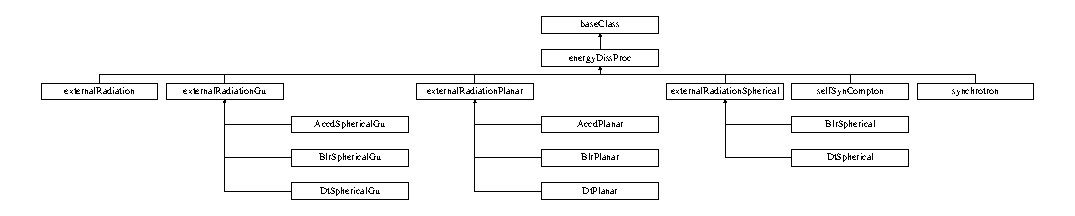
\includegraphics[height=2.456140cm]{classenergyDissProc}
\end{center}
\end{figure}


\subsection{Detailed Description}
Interface class for every energy dissipation process; provides memory management and other common methods shared by every process \subsection*{Public Member Functions}
\begin{DoxyCompactItemize}
\item 
\hyperlink{classenergyDissProc_a0cf0b423089016fbe8a697378c519590}{energy\-Diss\-Proc} (scfgp $\ast$\hyperlink{classbaseClass_a744f87a6ebe63da08256c022d42a4ca7}{cfg}, \hyperlink{classjetGeometry}{jet\-Geometry} $\ast$\hyperlink{classbaseClass_a482bb9b1d94f3eb3f31026d14e9a2bb6}{r}, \hyperlink{classelectrons}{electrons} $\ast$\hyperlink{classenergyDissProc_a0dbf0777938131e938c1fdad5df38a7f}{ele}, std\-::string \-\_\-id)
\item 
\hyperlink{classenergyDissProc_a0bef95f227129b0a24295451ae9464fd}{$\sim$energy\-Diss\-Proc} ()
\item 
virtual void \hyperlink{classenergyDissProc_a93a39df53f30801f9f057cd55c05485d}{set\-Lpv} ()
\item 
virtual double \hyperlink{classenergyDissProc_aed17a9ce8a970cbd1e250c59947407ac}{calculate\-Lpv} (double v)
\item 
virtual void \hyperlink{classenergyDissProc_a6033524ea3d0fe38056bd74622f6c4ad}{update} ()
\item 
virtual double \hyperlink{classenergyDissProc_a8074e0db5d859a8815e7136c2fc41b46}{dotg} (double g)
\item 
virtual void \hyperlink{classenergyDissProc_ad1fbde0f7635a19a81412b9766916eb9}{print\-Info} ()
\item 
void \hyperlink{classenergyDissProc_ab1f8b1a54a2e0b8ad36459c79fa719a2}{save\-Luminosity} ()
\item 
void \hyperlink{classenergyDissProc_a309e85da2d5f945980f9e5eb7afc65c0}{save\-Upe\-R} ()
\item 
\hypertarget{classenergyDissProc_a97b76448b8d2f476fe4caf43efe39353}{void {\bfseries allocate\-Lpv} ()}\label{classenergyDissProc_a97b76448b8d2f476fe4caf43efe39353}

\item 
\hypertarget{classenergyDissProc_aae94d4b633da390c21b8fe7c4a5b8aa2}{void {\bfseries allocate\-Lv\-Point} ()}\label{classenergyDissProc_aae94d4b633da390c21b8fe7c4a5b8aa2}

\item 
\hypertarget{classenergyDissProc_a3f7770c0f2f18b6d3db22addd2215aad}{void {\bfseries allocate\-Lv\-Point\-Avg} ()}\label{classenergyDissProc_a3f7770c0f2f18b6d3db22addd2215aad}

\item 
\hypertarget{classenergyDissProc_ab49630469fb4cbd85570e7c0fca3ebda}{void {\bfseries allocate\-Upe\-R} ()}\label{classenergyDissProc_ab49630469fb4cbd85570e7c0fca3ebda}

\item 
\hypertarget{classenergyDissProc_a1cc37afb4064270e6ea59735554284ca}{void {\bfseries allocate\-Upe} ()}\label{classenergyDissProc_a1cc37afb4064270e6ea59735554284ca}

\item 
\hypertarget{classenergyDissProc_ae29a12e9ce90130a2e76683ef9c5c6de}{void {\bfseries allocate\-Gamma\-K\-N} ()}\label{classenergyDissProc_ae29a12e9ce90130a2e76683ef9c5c6de}

\item 
\hypertarget{classenergyDissProc_ace7e2d8604c49806642f06cc5cffa300}{void {\bfseries free\-Lpv} ()}\label{classenergyDissProc_ace7e2d8604c49806642f06cc5cffa300}

\item 
\hypertarget{classenergyDissProc_a39d20e0e62bfe3dd3b98a598d24c2a78}{void {\bfseries free\-Lv\-Point} ()}\label{classenergyDissProc_a39d20e0e62bfe3dd3b98a598d24c2a78}

\item 
\hypertarget{classenergyDissProc_abdfac1c2548346152e32edd308fc08b9}{void {\bfseries free\-Lv\-Point\-Avg} ()}\label{classenergyDissProc_abdfac1c2548346152e32edd308fc08b9}

\item 
\hypertarget{classenergyDissProc_ad6f32ab9a7ebb77649a4c8a036f19b4a}{void {\bfseries free\-Upe} ()}\label{classenergyDissProc_ad6f32ab9a7ebb77649a4c8a036f19b4a}

\item 
\hypertarget{classenergyDissProc_a4f21c1b511d1460586c6a59551eeb35f}{void {\bfseries free\-Upe\-R} ()}\label{classenergyDissProc_a4f21c1b511d1460586c6a59551eeb35f}

\item 
\hypertarget{classenergyDissProc_a7d6d241fc80768e89a6e3967fe986b94}{void {\bfseries free\-Gamma\-K\-N} ()}\label{classenergyDissProc_a7d6d241fc80768e89a6e3967fe986b94}

\item 
\hypertarget{classenergyDissProc_ac1a5d2f5d3e4cd1cf71449a6dfe1c7da}{double {\bfseries get\-\_\-ep} (int i)}\label{classenergyDissProc_ac1a5d2f5d3e4cd1cf71449a6dfe1c7da}

\item 
\hypertarget{classenergyDissProc_a810aa6441b1e46c305f5470946512400}{double {\bfseries get\-\_\-upe} (int i)}\label{classenergyDissProc_a810aa6441b1e46c305f5470946512400}

\item 
\hypertarget{classenergyDissProc_a88f310d2f4e665d0082e5198128c3a67}{double {\bfseries get\-\_\-upe\-\_\-r} ()}\label{classenergyDissProc_a88f310d2f4e665d0082e5198128c3a67}

\item 
\hypertarget{classenergyDissProc_aa7e007d52f66e8ac3612ce7b6c11039d}{double {\bfseries get\-\_\-v\-Point} (int i)}\label{classenergyDissProc_aa7e007d52f66e8ac3612ce7b6c11039d}

\item 
\hypertarget{classenergyDissProc_aa8c9893ad2d0df90c0df7ef88b6a17b9}{double {\bfseries get\-\_\-\-Lv\-Point} (int i)}\label{classenergyDissProc_aa8c9893ad2d0df90c0df7ef88b6a17b9}

\item 
\hypertarget{classenergyDissProc_afc3e1ab967777ba9fb328c8dbfd42a4c}{double {\bfseries get\-\_\-\-Lv\-Point\-Avg} (int i)}\label{classenergyDissProc_afc3e1ab967777ba9fb328c8dbfd42a4c}

\item 
\hypertarget{classenergyDissProc_a43b078f6026c970fd87987aea954e220}{double {\bfseries get\-\_\-vp} (int i)}\label{classenergyDissProc_a43b078f6026c970fd87987aea954e220}

\item 
\hypertarget{classenergyDissProc_aed651aaf88e196cd8d225427a929dd95}{double {\bfseries get\-\_\-\-Lpv} (int i)}\label{classenergyDissProc_aed651aaf88e196cd8d225427a929dd95}

\item 
\hypertarget{classenergyDissProc_a8643da21bef260501b5ddc0548746126}{double {\bfseries get\-\_\-gamma\-K\-N} ()}\label{classenergyDissProc_a8643da21bef260501b5ddc0548746126}

\item 
\hypertarget{classenergyDissProc_ad2f07c8d60ebf53871000bad40b2cb40}{void {\bfseries set\-\_\-ep} (int i, double val)}\label{classenergyDissProc_ad2f07c8d60ebf53871000bad40b2cb40}

\item 
\hypertarget{classenergyDissProc_a1f27b82fc1dd725948bf3a29cab77372}{void {\bfseries set\-\_\-upe} (int i, double val)}\label{classenergyDissProc_a1f27b82fc1dd725948bf3a29cab77372}

\item 
\hypertarget{classenergyDissProc_a6b51c71d65457f34d351ec7299fbe732}{void {\bfseries set\-\_\-upe\-\_\-r} (double val)}\label{classenergyDissProc_a6b51c71d65457f34d351ec7299fbe732}

\item 
\hypertarget{classenergyDissProc_a46137d70a318966b6517432c10afc8d3}{void {\bfseries set\-\_\-v\-Point} (int i, double val)}\label{classenergyDissProc_a46137d70a318966b6517432c10afc8d3}

\item 
\hypertarget{classenergyDissProc_ace0f100af6f7034f5c3487f0cd6b9fd7}{void {\bfseries set\-\_\-\-Lv\-Point} (int i, double val)}\label{classenergyDissProc_ace0f100af6f7034f5c3487f0cd6b9fd7}

\item 
\hypertarget{classenergyDissProc_ae43c41e227b73a5205d9df5de1ede0d0}{void {\bfseries set\-\_\-\-Lv\-Point\-Avg} (int i, double val)}\label{classenergyDissProc_ae43c41e227b73a5205d9df5de1ede0d0}

\item 
\hypertarget{classenergyDissProc_a6a472066039c6a121e90010e66ac7535}{void {\bfseries set\-\_\-vp} (int i, double val)}\label{classenergyDissProc_a6a472066039c6a121e90010e66ac7535}

\item 
\hypertarget{classenergyDissProc_a59519f29627dcf510e7e268d138f2c53}{void {\bfseries set\-\_\-\-Lpv} (int i, double val)}\label{classenergyDissProc_a59519f29627dcf510e7e268d138f2c53}

\item 
\hypertarget{classenergyDissProc_a2d1d8edc34f87b276820c38e3c0dbd72}{double {\bfseries set\-\_\-gamma\-K\-N} (double val)}\label{classenergyDissProc_a2d1d8edc34f87b276820c38e3c0dbd72}

\item 
void \hyperlink{classenergyDissProc_a69ea4be814273e47e69e31e593c3a250}{set\-\_\-\-K\-N\-\_\-info} (double g)
\item 
void \hyperlink{classenergyDissProc_addd5bd336327bc4031644699cca16298}{print\-\_\-\-K\-N\-\_\-info} ()
\item 
double \hyperlink{classenergyDissProc_a5ef88d9ecacade52bbd277695230d237}{getd\-Log\-E} ()
\end{DoxyCompactItemize}
\subsection*{Public Attributes}
\begin{DoxyCompactItemize}
\item 
\hyperlink{classelectrons}{electrons} $\ast$ \hyperlink{classenergyDissProc_a0dbf0777938131e938c1fdad5df38a7f}{ele}
\item 
gsl\-\_\-vector $\ast$ \hyperlink{classenergyDissProc_a36330825cd7737639d5d223281b1c7e1}{ep}
\item 
gsl\-\_\-matrix $\ast$ \hyperlink{classenergyDissProc_aab57bc9681e8de22dc8a311e345bea53}{upe}
\item 
gsl\-\_\-vector $\ast$ \hyperlink{classenergyDissProc_abede39343a0a978c8dc8a064c80d6990}{vp}
\item 
gsl\-\_\-vector $\ast$ \hyperlink{classenergyDissProc_a235e694793915f34234654c58a0316b9}{Lpv}
\item 
gsl\-\_\-vector $\ast$ \hyperlink{classenergyDissProc_a1f075543ccaa902a20787c032822d8f4}{v\-Point}
\item 
gsl\-\_\-vector $\ast$ \hyperlink{classenergyDissProc_aa8463250da28ef23c71540b1efb24ee4}{Lv\-Point}
\item 
gsl\-\_\-vector $\ast$ \hyperlink{classenergyDissProc_a25546d40225b971c1b3dddb8e8f71258}{Lv\-Point\-Avg}
\item 
gsl\-\_\-vector $\ast$ \hyperlink{classenergyDissProc_ac925d66519c79f36421f75a6bc9f0965}{upe\-\_\-r}
\item 
double \hyperlink{classenergyDissProc_af1c1d91f8ef5f49f2f5831776052b651}{inj\-Rm}
\item 
int \hyperlink{classenergyDissProc_a2cc4e4eae15982f977a0dfa5458d80f4}{luminosity\-Const\-U}
\item 
int \hyperlink{classenergyDissProc_a0a23854c1c830dfb9ac33d116fce5b7d}{luminosity\-Const\-Nu}
\item 
gsl\-\_\-vector $\ast$ \hyperlink{classenergyDissProc_a22d892e2e11fc1f161ca3d0267752f9c}{gamma\-K\-N}
\item 
double \hyperlink{classenergyDissProc_a57aee74ef8fc4cb9220127a9c345174a}{ep\-Min}
\item 
\hypertarget{classenergyDissProc_ab55c8eafeef63eaaefe4eb82eef9b440}{double {\bfseries ep\-Max}}\label{classenergyDissProc_ab55c8eafeef63eaaefe4eb82eef9b440}

\item 
double \hyperlink{classenergyDissProc_aafedd3c012010a8e8aa34247660fea3b}{vp\-Min}
\item 
\hypertarget{classenergyDissProc_a5f9e91996d57a55a3508bd5596642a1e}{double {\bfseries vp\-Max}}\label{classenergyDissProc_a5f9e91996d57a55a3508bd5596642a1e}

\item 
double \hyperlink{classenergyDissProc_a270fdc20de5c26f9cc499f28dd32fb7b}{d\-Log\-E}
\item 
bool \hyperlink{classenergyDissProc_a7b51925f603e271657cab66afe822591}{flag\-\_\-upe\-\_\-r}
\end{DoxyCompactItemize}


\subsection{Constructor \& Destructor Documentation}
\hypertarget{classenergyDissProc_a0cf0b423089016fbe8a697378c519590}{\index{energy\-Diss\-Proc@{energy\-Diss\-Proc}!energy\-Diss\-Proc@{energy\-Diss\-Proc}}
\index{energy\-Diss\-Proc@{energy\-Diss\-Proc}!energyDissProc@{energy\-Diss\-Proc}}
\subsubsection[{energy\-Diss\-Proc}]{\setlength{\rightskip}{0pt plus 5cm}energy\-Diss\-Proc\-::energy\-Diss\-Proc (
\begin{DoxyParamCaption}
\item[{scfgp $\ast$}]{cfg, }
\item[{{\bf jet\-Geometry} $\ast$}]{r, }
\item[{{\bf electrons} $\ast$}]{ele, }
\item[{std\-::string}]{\-\_\-id}
\end{DoxyParamCaption}
)}}\label{classenergyDissProc_a0cf0b423089016fbe8a697378c519590}
constructor 
\begin{DoxyParams}{Parameters}
{\em scfgp} & \\
\hline
{\em \hyperlink{classjetGeometry}{jet\-Geometry}} & \\
\hline
{\em electrons} & \\
\hline
{\em id} & \\
\hline
\end{DoxyParams}

\begin{DoxyCode}
9                                                                                              : 
      \hyperlink{classbaseClass}{baseClass}(\_cfg, \_r, \_id ), \hyperlink{classenergyDissProc_a0dbf0777938131e938c1fdad5df38a7f}{ele}( \_ele ), \hyperlink{classenergyDissProc_a7b51925f603e271657cab66afe822591}{flag\_upe\_r}( \textcolor{keyword}{false} ) \{
10   
11   \textcolor{comment}{/* request parameters */}
12   \hyperlink{classbaseClass_a744f87a6ebe63da08256c022d42a4ca7}{cfg} -> request<int>(\textcolor{stringliteral}{"saveLum"},0,&saveLum);
13   \hyperlink{classbaseClass_a744f87a6ebe63da08256c022d42a4ca7}{cfg} -> request<int>(\textcolor{stringliteral}{"saveUpeVsR"},0,&saveUpeVsR);
14   \hyperlink{classbaseClass_a744f87a6ebe63da08256c022d42a4ca7}{cfg} -> request<double>(\textcolor{stringliteral}{"injRm"},2.0e17,&\hyperlink{classenergyDissProc_af1c1d91f8ef5f49f2f5831776052b651}{injRm});
15   
16   \hyperlink{classbaseClass_a744f87a6ebe63da08256c022d42a4ca7}{cfg} -> updateRequests( );
17 
18   \textcolor{comment}{/* allocate common memory */}
19   allocateGammaKN(); \}
\end{DoxyCode}
\hypertarget{classenergyDissProc_a0bef95f227129b0a24295451ae9464fd}{\index{energy\-Diss\-Proc@{energy\-Diss\-Proc}!$\sim$energy\-Diss\-Proc@{$\sim$energy\-Diss\-Proc}}
\index{$\sim$energy\-Diss\-Proc@{$\sim$energy\-Diss\-Proc}!energyDissProc@{energy\-Diss\-Proc}}
\subsubsection[{$\sim$energy\-Diss\-Proc}]{\setlength{\rightskip}{0pt plus 5cm}energy\-Diss\-Proc\-::$\sim$energy\-Diss\-Proc (
\begin{DoxyParamCaption}
{}
\end{DoxyParamCaption}
)}}\label{classenergyDissProc_a0bef95f227129b0a24295451ae9464fd}
destructor 
\begin{DoxyCode}
21                                  \{
22   freeGammaKN( );
23   \hyperlink{classenergyDissProc_a0dbf0777938131e938c1fdad5df38a7f}{ele} = NULL; \}
\end{DoxyCode}


\subsection{Member Function Documentation}
\hypertarget{classenergyDissProc_aed17a9ce8a970cbd1e250c59947407ac}{\index{energy\-Diss\-Proc@{energy\-Diss\-Proc}!calculate\-Lpv@{calculate\-Lpv}}
\index{calculate\-Lpv@{calculate\-Lpv}!energyDissProc@{energy\-Diss\-Proc}}
\subsubsection[{calculate\-Lpv}]{\setlength{\rightskip}{0pt plus 5cm}virtual double energy\-Diss\-Proc\-::calculate\-Lpv (
\begin{DoxyParamCaption}
\item[{double}]{v}
\end{DoxyParamCaption}
)\hspace{0.3cm}{\ttfamily [inline]}, {\ttfamily [virtual]}}}\label{classenergyDissProc_aed17a9ce8a970cbd1e250c59947407ac}
calculate intrinsic luminosity 
\begin{DoxyParams}{Parameters}
{\em v} & -\/ frequency (jet co-\/moving frame) \\
\hline
\end{DoxyParams}
\begin{DoxyReturn}{Returns}
L'\-\_\-v 
\end{DoxyReturn}


Reimplemented in \hyperlink{classsynchrotron_ab12acf6ee2bdc60011e2739ba42cd32a}{synchrotron}, and \hyperlink{classselfSynCompton_a39e8b6e7b4094f39f9436cd94a15775e}{self\-Syn\-Compton}.


\begin{DoxyCode}
86 \{ \};
\end{DoxyCode}
\hypertarget{classenergyDissProc_a8074e0db5d859a8815e7136c2fc41b46}{\index{energy\-Diss\-Proc@{energy\-Diss\-Proc}!dotg@{dotg}}
\index{dotg@{dotg}!energyDissProc@{energy\-Diss\-Proc}}
\subsubsection[{dotg}]{\setlength{\rightskip}{0pt plus 5cm}virtual double energy\-Diss\-Proc\-::dotg (
\begin{DoxyParamCaption}
\item[{double}]{g}
\end{DoxyParamCaption}
)\hspace{0.3cm}{\ttfamily [inline]}, {\ttfamily [virtual]}}}\label{classenergyDissProc_a8074e0db5d859a8815e7136c2fc41b46}
get d gamma \textbackslash{} d t for particular process 
\begin{DoxyParams}{Parameters}
{\em g} & -\/ electron Lorentz factor \\
\hline
\end{DoxyParams}
\begin{DoxyReturn}{Returns}
d gamma \textbackslash{} d t 
\end{DoxyReturn}


Reimplemented in \hyperlink{classexternalRadiationPlanar_a4f49eec94e9d935df18534fe021c750c}{external\-Radiation\-Planar}, \hyperlink{classexternalRadiationSpherical_a96a2857022de4cc79852824610943910}{external\-Radiation\-Spherical}, \hyperlink{classexternalRadiationGu_a266fc022608ea384a80be8ad840d5957}{external\-Radiation\-Gu}, \hyperlink{classsynchrotron_a577e2fa11ba90bf288099e88f02c756f}{synchrotron}, \hyperlink{classselfSynCompton_a51bad50f11e56a623b80e4436ef1b629}{self\-Syn\-Compton}, and \hyperlink{classexternalRadiation_af3011c765884717fac63035c51c4b0a2}{external\-Radiation}.


\begin{DoxyCode}
94 \{ \};
\end{DoxyCode}
\hypertarget{classenergyDissProc_a5ef88d9ecacade52bbd277695230d237}{\index{energy\-Diss\-Proc@{energy\-Diss\-Proc}!getd\-Log\-E@{getd\-Log\-E}}
\index{getd\-Log\-E@{getd\-Log\-E}!energyDissProc@{energy\-Diss\-Proc}}
\subsubsection[{getd\-Log\-E}]{\setlength{\rightskip}{0pt plus 5cm}double energy\-Diss\-Proc\-::getd\-Log\-E (
\begin{DoxyParamCaption}
{}
\end{DoxyParamCaption}
)\hspace{0.3cm}{\ttfamily [inline]}}}\label{classenergyDissProc_a5ef88d9ecacade52bbd277695230d237}
get log-\/energy step \begin{DoxyReturn}{Returns}
log-\/energy step 
\end{DoxyReturn}

\begin{DoxyCode}
152 \{ \textcolor{keywordflow}{return} \hyperlink{classenergyDissProc_a270fdc20de5c26f9cc499f28dd32fb7b}{dLogE}; \}
\end{DoxyCode}
\hypertarget{classenergyDissProc_addd5bd336327bc4031644699cca16298}{\index{energy\-Diss\-Proc@{energy\-Diss\-Proc}!print\-\_\-\-K\-N\-\_\-info@{print\-\_\-\-K\-N\-\_\-info}}
\index{print\-\_\-\-K\-N\-\_\-info@{print\-\_\-\-K\-N\-\_\-info}!energyDissProc@{energy\-Diss\-Proc}}
\subsubsection[{print\-\_\-\-K\-N\-\_\-info}]{\setlength{\rightskip}{0pt plus 5cm}void energy\-Diss\-Proc\-::print\-\_\-\-K\-N\-\_\-info (
\begin{DoxyParamCaption}
{}
\end{DoxyParamCaption}
)}}\label{classenergyDissProc_addd5bd336327bc4031644699cca16298}
print info whether particular process for particular electron energy is withing Klein-\/\-Nishina region already 
\begin{DoxyCode}
96                                     \{ 
97   std::cout << \textcolor{stringliteral}{" KN info "}+this->\hyperlink{classbaseClass_a756d5accf10ced9a34024048c95a51c9}{whoAmI}() << \textcolor{stringliteral}{"\(\backslash\)tradius: "} << \hyperlink{classbaseClass_a482bb9b1d94f3eb3f31026d14e9a2bb6}{r}->get() << \textcolor{stringliteral}{"\(\backslash\)tgammaKN: "};
98   \textcolor{keywordflow}{if}( get\_gammaKN() > \hyperlink{classenergyDissProc_a0dbf0777938131e938c1fdad5df38a7f}{ele}->getGammaMax( ) || get\_gammaKN( ) == 0.0 ) \{
99     std::cout << \textcolor{stringliteral}{"> gammaMax = "} << std::scientific << std::setprecision(2) << 
      \hyperlink{classenergyDissProc_a0dbf0777938131e938c1fdad5df38a7f}{ele}->getGammaMax( ) << std::endl; \}
100   \textcolor{keywordflow}{else} \{ std::cout << std::scientific << std::setprecision(2) << get\_gammaKN() << std::endl; \}
101 \}
\end{DoxyCode}
\hypertarget{classenergyDissProc_ad1fbde0f7635a19a81412b9766916eb9}{\index{energy\-Diss\-Proc@{energy\-Diss\-Proc}!print\-Info@{print\-Info}}
\index{print\-Info@{print\-Info}!energyDissProc@{energy\-Diss\-Proc}}
\subsubsection[{print\-Info}]{\setlength{\rightskip}{0pt plus 5cm}virtual void energy\-Diss\-Proc\-::print\-Info (
\begin{DoxyParamCaption}
{}
\end{DoxyParamCaption}
)\hspace{0.3cm}{\ttfamily [inline]}, {\ttfamily [virtual]}}}\label{classenergyDissProc_ad1fbde0f7635a19a81412b9766916eb9}
print basic information about myself (virtual) 

Reimplemented from \hyperlink{classbaseClass_a67f911cca483b620b908c69dfa4f3ad7}{base\-Class}.



Reimplemented in \hyperlink{classexternalRadiationPlanar_a47e497b12dfa4e71311bffb3a4b384b2}{external\-Radiation\-Planar}, \hyperlink{classDtSpherical_a14440ec30b997fe2461c07f4507dd994}{Dt\-Spherical}, \hyperlink{classBlrPlanar_a3321d83625869e16c5794d9419dff073}{Blr\-Planar}, \hyperlink{classsynchrotron_a6a8610b523a6e3c656372537ad28b756}{synchrotron}, \hyperlink{classBlrSpherical_a101b95271855f15f1049fcea9efde235}{Blr\-Spherical}, \hyperlink{classexternalRadiationSpherical_a232684df0d246d8c5ec06e832bbaad0f}{external\-Radiation\-Spherical}, \hyperlink{classDtPlanar_a0d1b6697d54a08030ed50b7e4b5fbfef}{Dt\-Planar}, \hyperlink{classselfSynCompton_a46f692985a0fd74c14a018cc43f25c0b}{self\-Syn\-Compton}, \hyperlink{classAccdPlanar_a51960bc05d15aedf068b65a369d1899c}{Accd\-Planar}, \hyperlink{classexternalRadiationGu_a8aa28d939b0ecf2651f18cc4f5f6ba25}{external\-Radiation\-Gu}, \hyperlink{classBlrSphericalGu_a69de552417b7b01c3634650aaa9413d7}{Blr\-Spherical\-Gu}, \hyperlink{classDtSphericalGu_aeed0bda6440570b686aaf85bf5d2b6b3}{Dt\-Spherical\-Gu}, \hyperlink{classAccdSphericalGu_a672f673606422556c3fb31a1787c6724}{Accd\-Spherical\-Gu}, and \hyperlink{classexternalRadiation_a8747348f3468165fca0c5547e207b5a9}{external\-Radiation}.


\begin{DoxyCode}
95 \{ \};
\end{DoxyCode}
\hypertarget{classenergyDissProc_ab1f8b1a54a2e0b8ad36459c79fa719a2}{\index{energy\-Diss\-Proc@{energy\-Diss\-Proc}!save\-Luminosity@{save\-Luminosity}}
\index{save\-Luminosity@{save\-Luminosity}!energyDissProc@{energy\-Diss\-Proc}}
\subsubsection[{save\-Luminosity}]{\setlength{\rightskip}{0pt plus 5cm}void energy\-Diss\-Proc\-::save\-Luminosity (
\begin{DoxyParamCaption}
{}
\end{DoxyParamCaption}
)}}\label{classenergyDissProc_ab1f8b1a54a2e0b8ad36459c79fa719a2}
save calulated luminosity 
\begin{DoxyCode}
103                                      \{
104   std::string type = \textcolor{stringliteral}{"Lpv\_"}+this->\hyperlink{classbaseClass_a756d5accf10ced9a34024048c95a51c9}{whoAmI}( );
105   bazinga::info(this->\hyperlink{classbaseClass_a756d5accf10ced9a34024048c95a51c9}{whoAmI}( ),\textcolor{stringliteral}{"Saving luminosity."});
106   \textcolor{keywordflow}{if}( saveLum && \hyperlink{classbaseClass_a482bb9b1d94f3eb3f31026d14e9a2bb6}{r}->ifSaveRadius( ) ) \{ bazinga::save\_GSLVector( type, this->\hyperlink{classenergyDissProc_abede39343a0a978c8dc8a064c80d6990}{vp}, 
      \hyperlink{classenergyDissProc_a0dbf0777938131e938c1fdad5df38a7f}{ele}->\hyperlink{classelectrons_aba72b6575be27358efcb13cc3415df68}{gamma}, this->Lpv, \hyperlink{classbaseClass_a482bb9b1d94f3eb3f31026d14e9a2bb6}{r}->getPosition( ), \hyperlink{classbaseClass_a744f87a6ebe63da08256c022d42a4ca7}{cfg}->get<std::string>(\textcolor{stringliteral}{"output"}) ); \}
107 \}
\end{DoxyCode}
\hypertarget{classenergyDissProc_a309e85da2d5f945980f9e5eb7afc65c0}{\index{energy\-Diss\-Proc@{energy\-Diss\-Proc}!save\-Upe\-R@{save\-Upe\-R}}
\index{save\-Upe\-R@{save\-Upe\-R}!energyDissProc@{energy\-Diss\-Proc}}
\subsubsection[{save\-Upe\-R}]{\setlength{\rightskip}{0pt plus 5cm}void energy\-Diss\-Proc\-::save\-Upe\-R (
\begin{DoxyParamCaption}
{}
\end{DoxyParamCaption}
)}}\label{classenergyDissProc_a309e85da2d5f945980f9e5eb7afc65c0}
save energy density vs radius info 
\begin{DoxyCode}
109                                \{
110   std::string type = \textcolor{stringliteral}{"UpeR\_"}+this->\hyperlink{classbaseClass_a756d5accf10ced9a34024048c95a51c9}{whoAmI}( );
111   bazinga::info(this->\hyperlink{classbaseClass_a756d5accf10ced9a34024048c95a51c9}{whoAmI}( ),\textcolor{stringliteral}{"Saving upe vs radius info."});
112   \textcolor{keywordflow}{if}( saveUpeVsR ) \{ bazinga::save\_GSLVector( type, \hyperlink{classbaseClass_a482bb9b1d94f3eb3f31026d14e9a2bb6}{r}->getRadius\_GSLVector( ), this->
      \hyperlink{classenergyDissProc_ac925d66519c79f36421f75a6bc9f0965}{upe\_r}, \hyperlink{classbaseClass_a744f87a6ebe63da08256c022d42a4ca7}{cfg}->get<std::string>(\textcolor{stringliteral}{"output"}) ); \}
113 \}
\end{DoxyCode}
\hypertarget{classenergyDissProc_a69ea4be814273e47e69e31e593c3a250}{\index{energy\-Diss\-Proc@{energy\-Diss\-Proc}!set\-\_\-\-K\-N\-\_\-info@{set\-\_\-\-K\-N\-\_\-info}}
\index{set\-\_\-\-K\-N\-\_\-info@{set\-\_\-\-K\-N\-\_\-info}!energyDissProc@{energy\-Diss\-Proc}}
\subsubsection[{set\-\_\-\-K\-N\-\_\-info}]{\setlength{\rightskip}{0pt plus 5cm}void energy\-Diss\-Proc\-::set\-\_\-\-K\-N\-\_\-info (
\begin{DoxyParamCaption}
\item[{double}]{g}
\end{DoxyParamCaption}
)}}\label{classenergyDissProc_a69ea4be814273e47e69e31e593c3a250}
set information about Klein-\/\-Nishina regime 
\begin{DoxyParams}{Parameters}
{\em -\/} & electron Lorentz factor \\
\hline
\end{DoxyParams}

\begin{DoxyCode}
91                                            \{
92   \textcolor{keywordflow}{if}( get\_gammaKN( ) == 0 ) \{ set\_gammaKN( g ); \}
93   \textcolor{keywordflow}{else} \textcolor{keywordflow}{if}( get\_gammaKN( ) > g ) \{ set\_gammaKN( g ); \}
94 \}
\end{DoxyCode}
\hypertarget{classenergyDissProc_a93a39df53f30801f9f057cd55c05485d}{\index{energy\-Diss\-Proc@{energy\-Diss\-Proc}!set\-Lpv@{set\-Lpv}}
\index{set\-Lpv@{set\-Lpv}!energyDissProc@{energy\-Diss\-Proc}}
\subsubsection[{set\-Lpv}]{\setlength{\rightskip}{0pt plus 5cm}virtual void energy\-Diss\-Proc\-::set\-Lpv (
\begin{DoxyParamCaption}
{}
\end{DoxyParamCaption}
)\hspace{0.3cm}{\ttfamily [inline]}, {\ttfamily [virtual]}}}\label{classenergyDissProc_a93a39df53f30801f9f057cd55c05485d}
set intrinsic luminosities 

Reimplemented in \hyperlink{classexternalRadiationPlanar_a8023104635baec445f038e9f1ca6c3bc}{external\-Radiation\-Planar}, \hyperlink{classexternalRadiationSpherical_a2868df3597900f03c135baef15c825a8}{external\-Radiation\-Spherical}, \hyperlink{classexternalRadiationGu_a946369eee3485a821a5619c5ba310497}{external\-Radiation\-Gu}, \hyperlink{classsynchrotron_adf30d0e7cbba05a39a16b60957d02321}{synchrotron}, \hyperlink{classselfSynCompton_ae34a13d5ddf894d3e1ede229ffb4176a}{self\-Syn\-Compton}, and \hyperlink{classexternalRadiation_a57048bff39c56bb1d9ec1e9c88d39323}{external\-Radiation}.


\begin{DoxyCode}
81 \{ \};
\end{DoxyCode}
\hypertarget{classenergyDissProc_a6033524ea3d0fe38056bd74622f6c4ad}{\index{energy\-Diss\-Proc@{energy\-Diss\-Proc}!update@{update}}
\index{update@{update}!energyDissProc@{energy\-Diss\-Proc}}
\subsubsection[{update}]{\setlength{\rightskip}{0pt plus 5cm}virtual void energy\-Diss\-Proc\-::update (
\begin{DoxyParamCaption}
{}
\end{DoxyParamCaption}
)\hspace{0.3cm}{\ttfamily [inline]}, {\ttfamily [virtual]}}}\label{classenergyDissProc_a6033524ea3d0fe38056bd74622f6c4ad}
update all process internal parameters to current radius 

Reimplemented in \hyperlink{classexternalRadiationPlanar_acfddae49394d11c89d1d47229ba8a3f7}{external\-Radiation\-Planar}, \hyperlink{classsynchrotron_a52ec26284de15395bd203037024b7ae4}{synchrotron}, \hyperlink{classDtSpherical_ab9844cfdd3df5bc213bf93dd7b320bb7}{Dt\-Spherical}, \hyperlink{classexternalRadiationSpherical_a05f5cf91c3a3c7844b167ff4476e64f8}{external\-Radiation\-Spherical}, \hyperlink{classselfSynCompton_af254f0dcd2abfe1d218c85d917992e24}{self\-Syn\-Compton}, \hyperlink{classBlrSpherical_ad67ab24f0b7f0ec3a0893fd2e3170f6c}{Blr\-Spherical}, \hyperlink{classexternalRadiationGu_a730363f393f29aef9927e0bb84087116}{external\-Radiation\-Gu}, \hyperlink{classBlrSphericalGu_a0054a1bc21351e6d68b8b5190ab1a8b0}{Blr\-Spherical\-Gu}, \hyperlink{classDtSphericalGu_ac940befec9ea9886b136f9d96c88620a}{Dt\-Spherical\-Gu}, \hyperlink{classAccdSphericalGu_a278cae9b07c99dd7398121a77fa069c9}{Accd\-Spherical\-Gu}, and \hyperlink{classexternalRadiation_aa458ea6aefe596525520b06fd6065ffd}{external\-Radiation}.


\begin{DoxyCode}
89 \{ \};
\end{DoxyCode}


\subsection{Member Data Documentation}
\hypertarget{classenergyDissProc_a270fdc20de5c26f9cc499f28dd32fb7b}{\index{energy\-Diss\-Proc@{energy\-Diss\-Proc}!d\-Log\-E@{d\-Log\-E}}
\index{d\-Log\-E@{d\-Log\-E}!energyDissProc@{energy\-Diss\-Proc}}
\subsubsection[{d\-Log\-E}]{\setlength{\rightskip}{0pt plus 5cm}double energy\-Diss\-Proc\-::d\-Log\-E}}\label{classenergyDissProc_a270fdc20de5c26f9cc499f28dd32fb7b}
ep integration step \hypertarget{classenergyDissProc_a0dbf0777938131e938c1fdad5df38a7f}{\index{energy\-Diss\-Proc@{energy\-Diss\-Proc}!ele@{ele}}
\index{ele@{ele}!energyDissProc@{energy\-Diss\-Proc}}
\subsubsection[{ele}]{\setlength{\rightskip}{0pt plus 5cm}{\bf electrons}$\ast$ energy\-Diss\-Proc\-::ele}}\label{classenergyDissProc_a0dbf0777938131e938c1fdad5df38a7f}
class needs to have access to electrons to calculate luminosities etc \hypertarget{classenergyDissProc_a36330825cd7737639d5d223281b1c7e1}{\index{energy\-Diss\-Proc@{energy\-Diss\-Proc}!ep@{ep}}
\index{ep@{ep}!energyDissProc@{energy\-Diss\-Proc}}
\subsubsection[{ep}]{\setlength{\rightskip}{0pt plus 5cm}gsl\-\_\-vector$\ast$ energy\-Diss\-Proc\-::ep}}\label{classenergyDissProc_a36330825cd7737639d5d223281b1c7e1}
data matrices and vectors; first index is radius photon field energy -\/ primed \hypertarget{classenergyDissProc_a57aee74ef8fc4cb9220127a9c345174a}{\index{energy\-Diss\-Proc@{energy\-Diss\-Proc}!ep\-Min@{ep\-Min}}
\index{ep\-Min@{ep\-Min}!energyDissProc@{energy\-Diss\-Proc}}
\subsubsection[{ep\-Min}]{\setlength{\rightskip}{0pt plus 5cm}double energy\-Diss\-Proc\-::ep\-Min}}\label{classenergyDissProc_a57aee74ef8fc4cb9220127a9c345174a}
boundary energies \hypertarget{classenergyDissProc_a7b51925f603e271657cab66afe822591}{\index{energy\-Diss\-Proc@{energy\-Diss\-Proc}!flag\-\_\-upe\-\_\-r@{flag\-\_\-upe\-\_\-r}}
\index{flag\-\_\-upe\-\_\-r@{flag\-\_\-upe\-\_\-r}!energyDissProc@{energy\-Diss\-Proc}}
\subsubsection[{flag\-\_\-upe\-\_\-r}]{\setlength{\rightskip}{0pt plus 5cm}bool energy\-Diss\-Proc\-::flag\-\_\-upe\-\_\-r}}\label{classenergyDissProc_a7b51925f603e271657cab66afe822591}
set this to true after setting upe\-\_\-r \hypertarget{classenergyDissProc_a22d892e2e11fc1f161ca3d0267752f9c}{\index{energy\-Diss\-Proc@{energy\-Diss\-Proc}!gamma\-K\-N@{gamma\-K\-N}}
\index{gamma\-K\-N@{gamma\-K\-N}!energyDissProc@{energy\-Diss\-Proc}}
\subsubsection[{gamma\-K\-N}]{\setlength{\rightskip}{0pt plus 5cm}gsl\-\_\-vector$\ast$ energy\-Diss\-Proc\-::gamma\-K\-N}}\label{classenergyDissProc_a22d892e2e11fc1f161ca3d0267752f9c}
data vector to store information on electrons energies that cool in the Klein-\/\-Nishina regime for each radius a data on electrons in K\-N in being saved \hypertarget{classenergyDissProc_af1c1d91f8ef5f49f2f5831776052b651}{\index{energy\-Diss\-Proc@{energy\-Diss\-Proc}!inj\-Rm@{inj\-Rm}}
\index{inj\-Rm@{inj\-Rm}!energyDissProc@{energy\-Diss\-Proc}}
\subsubsection[{inj\-Rm}]{\setlength{\rightskip}{0pt plus 5cm}double energy\-Diss\-Proc\-::inj\-Rm}}\label{classenergyDissProc_af1c1d91f8ef5f49f2f5831776052b651}
used to specify radial maximum of injected electrons -\/ used only for non-\/uniform injections \hypertarget{classenergyDissProc_a235e694793915f34234654c58a0316b9}{\index{energy\-Diss\-Proc@{energy\-Diss\-Proc}!Lpv@{Lpv}}
\index{Lpv@{Lpv}!energyDissProc@{energy\-Diss\-Proc}}
\subsubsection[{Lpv}]{\setlength{\rightskip}{0pt plus 5cm}gsl\-\_\-vector$\ast$ energy\-Diss\-Proc\-::\-Lpv}}\label{classenergyDissProc_a235e694793915f34234654c58a0316b9}
monochromatic apparent luminosity -\/ primed \hypertarget{classenergyDissProc_a0a23854c1c830dfb9ac33d116fce5b7d}{\index{energy\-Diss\-Proc@{energy\-Diss\-Proc}!luminosity\-Const\-Nu@{luminosity\-Const\-Nu}}
\index{luminosity\-Const\-Nu@{luminosity\-Const\-Nu}!energyDissProc@{energy\-Diss\-Proc}}
\subsubsection[{luminosity\-Const\-Nu}]{\setlength{\rightskip}{0pt plus 5cm}int energy\-Diss\-Proc\-::luminosity\-Const\-Nu}}\label{classenergyDissProc_a0a23854c1c830dfb9ac33d116fce5b7d}
set this to 1 if luminosity is to be calculated with constant v'; in such case v' will be set to a constant value given by v'(injrm) \hypertarget{classenergyDissProc_a2cc4e4eae15982f977a0dfa5458d80f4}{\index{energy\-Diss\-Proc@{energy\-Diss\-Proc}!luminosity\-Const\-U@{luminosity\-Const\-U}}
\index{luminosity\-Const\-U@{luminosity\-Const\-U}!energyDissProc@{energy\-Diss\-Proc}}
\subsubsection[{luminosity\-Const\-U}]{\setlength{\rightskip}{0pt plus 5cm}int energy\-Diss\-Proc\-::luminosity\-Const\-U}}\label{classenergyDissProc_a2cc4e4eae15982f977a0dfa5458d80f4}
set this to 1 if luminosity is to be calculated with constant u\-\_\-ext; in such case u' will be set to a constant value given by u'(injrm) \hypertarget{classenergyDissProc_aa8463250da28ef23c71540b1efb24ee4}{\index{energy\-Diss\-Proc@{energy\-Diss\-Proc}!Lv\-Point@{Lv\-Point}}
\index{Lv\-Point@{Lv\-Point}!energyDissProc@{energy\-Diss\-Proc}}
\subsubsection[{Lv\-Point}]{\setlength{\rightskip}{0pt plus 5cm}gsl\-\_\-vector$\ast$ energy\-Diss\-Proc\-::\-Lv\-Point}}\label{classenergyDissProc_aa8463250da28ef23c71540b1efb24ee4}
monochromatic apparent luminosity for point source \hypertarget{classenergyDissProc_a25546d40225b971c1b3dddb8e8f71258}{\index{energy\-Diss\-Proc@{energy\-Diss\-Proc}!Lv\-Point\-Avg@{Lv\-Point\-Avg}}
\index{Lv\-Point\-Avg@{Lv\-Point\-Avg}!energyDissProc@{energy\-Diss\-Proc}}
\subsubsection[{Lv\-Point\-Avg}]{\setlength{\rightskip}{0pt plus 5cm}gsl\-\_\-vector$\ast$ energy\-Diss\-Proc\-::\-Lv\-Point\-Avg}}\label{classenergyDissProc_a25546d40225b971c1b3dddb8e8f71258}
monochromatic apparent luminosity for point source averaged over radius \hypertarget{classenergyDissProc_aab57bc9681e8de22dc8a311e345bea53}{\index{energy\-Diss\-Proc@{energy\-Diss\-Proc}!upe@{upe}}
\index{upe@{upe}!energyDissProc@{energy\-Diss\-Proc}}
\subsubsection[{upe}]{\setlength{\rightskip}{0pt plus 5cm}gsl\-\_\-matrix$\ast$ energy\-Diss\-Proc\-::upe}}\label{classenergyDissProc_aab57bc9681e8de22dc8a311e345bea53}
photon field monochromatic energy density -\/ primed \hypertarget{classenergyDissProc_ac925d66519c79f36421f75a6bc9f0965}{\index{energy\-Diss\-Proc@{energy\-Diss\-Proc}!upe\-\_\-r@{upe\-\_\-r}}
\index{upe\-\_\-r@{upe\-\_\-r}!energyDissProc@{energy\-Diss\-Proc}}
\subsubsection[{upe\-\_\-r}]{\setlength{\rightskip}{0pt plus 5cm}gsl\-\_\-vector$\ast$ energy\-Diss\-Proc\-::upe\-\_\-r}}\label{classenergyDissProc_ac925d66519c79f36421f75a6bc9f0965}
data vector for storing energy density vs radius \hypertarget{classenergyDissProc_abede39343a0a978c8dc8a064c80d6990}{\index{energy\-Diss\-Proc@{energy\-Diss\-Proc}!vp@{vp}}
\index{vp@{vp}!energyDissProc@{energy\-Diss\-Proc}}
\subsubsection[{vp}]{\setlength{\rightskip}{0pt plus 5cm}gsl\-\_\-vector$\ast$ energy\-Diss\-Proc\-::vp}}\label{classenergyDissProc_abede39343a0a978c8dc8a064c80d6990}
frequency -\/ primed \hypertarget{classenergyDissProc_aafedd3c012010a8e8aa34247660fea3b}{\index{energy\-Diss\-Proc@{energy\-Diss\-Proc}!vp\-Min@{vp\-Min}}
\index{vp\-Min@{vp\-Min}!energyDissProc@{energy\-Diss\-Proc}}
\subsubsection[{vp\-Min}]{\setlength{\rightskip}{0pt plus 5cm}double energy\-Diss\-Proc\-::vp\-Min}}\label{classenergyDissProc_aafedd3c012010a8e8aa34247660fea3b}
boundary frequencies \hypertarget{classenergyDissProc_a1f075543ccaa902a20787c032822d8f4}{\index{energy\-Diss\-Proc@{energy\-Diss\-Proc}!v\-Point@{v\-Point}}
\index{v\-Point@{v\-Point}!energyDissProc@{energy\-Diss\-Proc}}
\subsubsection[{v\-Point}]{\setlength{\rightskip}{0pt plus 5cm}gsl\-\_\-vector$\ast$ energy\-Diss\-Proc\-::v\-Point}}\label{classenergyDissProc_a1f075543ccaa902a20787c032822d8f4}
freqency -\/ point source 

The documentation for this class was generated from the following files\-:\begin{DoxyCompactItemize}
\item 
/home/mjaniak/\-Soft/blazar++/include/\hyperlink{energyDissProc_8hpp}{energy\-Diss\-Proc.\-hpp}\item 
/home/mjaniak/\-Soft/blazar++/src/\hyperlink{energyDissProc_8cpp}{energy\-Diss\-Proc.\-cpp}\end{DoxyCompactItemize}

\hypertarget{classexternalRadiation}{\section{external\-Radiation Class Reference}
\label{classexternalRadiation}\index{external\-Radiation@{external\-Radiation}}
}
Inheritance diagram for external\-Radiation\-:\begin{figure}[H]
\begin{center}
\leavevmode
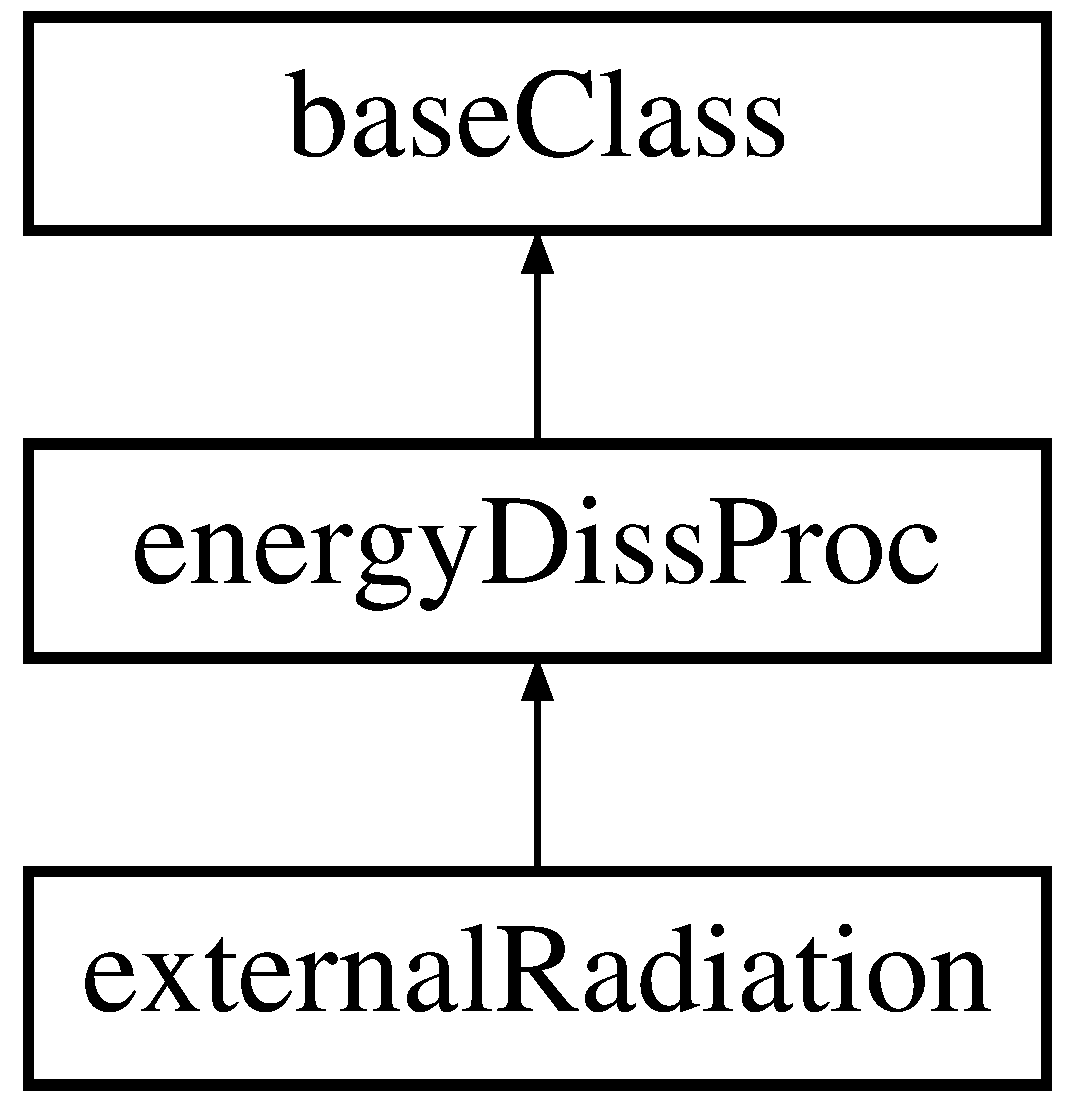
\includegraphics[height=3.000000cm]{classexternalRadiation}
\end{center}
\end{figure}
\subsection*{Public Member Functions}
\begin{DoxyCompactItemize}
\item 
\hypertarget{classexternalRadiation_af5a905e2a45845747dfcb1035ed69069}{{\bfseries external\-Radiation} (scfgp $\ast$\-\_\-cfg, \hyperlink{classjetGeometry}{jet\-Geometry} $\ast$\-\_\-r, \hyperlink{classelectrons}{electrons} $\ast$\-\_\-ele, std\-::string \-\_\-id)}\label{classexternalRadiation_af5a905e2a45845747dfcb1035ed69069}

\item 
double \hyperlink{classexternalRadiation_af3011c765884717fac63035c51c4b0a2}{dotg} (double g)
\item 
void \hyperlink{classexternalRadiation_aa458ea6aefe596525520b06fd6065ffd}{update} ()
\item 
void \hyperlink{classexternalRadiation_a57048bff39c56bb1d9ec1e9c88d39323}{set\-Lpv} ()
\item 
\hypertarget{classexternalRadiation_a7ee57d513164aff07202d27b743406c9}{double {\bfseries calculate\-Lpv} (double v, double theta)}\label{classexternalRadiation_a7ee57d513164aff07202d27b743406c9}

\item 
void \hyperlink{classexternalRadiation_a8747348f3468165fca0c5547e207b5a9}{print\-Info} ()
\end{DoxyCompactItemize}
\subsection*{Additional Inherited Members}


\subsection{Member Function Documentation}
\hypertarget{classexternalRadiation_af3011c765884717fac63035c51c4b0a2}{\index{external\-Radiation@{external\-Radiation}!dotg@{dotg}}
\index{dotg@{dotg}!externalRadiation@{external\-Radiation}}
\subsubsection[{dotg}]{\setlength{\rightskip}{0pt plus 5cm}double external\-Radiation\-::dotg (
\begin{DoxyParamCaption}
\item[{double}]{g}
\end{DoxyParamCaption}
)\hspace{0.3cm}{\ttfamily [virtual]}}}\label{classexternalRadiation_af3011c765884717fac63035c51c4b0a2}
get d gamma \textbackslash{} d t for particular process 
\begin{DoxyParams}{Parameters}
{\em g} & -\/ electron Lorentz factor \\
\hline
\end{DoxyParams}
\begin{DoxyReturn}{Returns}
d gamma \textbackslash{} d t 
\end{DoxyReturn}


Reimplemented from \hyperlink{classenergyDissProc_a8074e0db5d859a8815e7136c2fc41b46}{energy\-Diss\-Proc}.


\begin{DoxyCode}
72                                          \{
73   \textcolor{keywordtype}{double} b, sum, val = 0.0;
74   \textcolor{keywordflow}{for}( \textcolor{keywordtype}{int} i=0;i<\hyperlink{classbaseClass_a2b4d07d2b46197d495de0477f4bb22f8}{N};i++ ) \{
75       b = 4.0*get\_ep(i)*g;
76       \textcolor{keywordflow}{if}( b > 1.0 ) \{ \hyperlink{classenergyDissProc_a69ea4be814273e47e69e31e593c3a250}{set\_KN\_info}( g ); \}
77       sum += bazinga::IntCor(i,N)*get\_ep(i)*get\_upe(i)*inverseCompton::fKN(b,KN); \}
78 
79   val = \hyperlink{classenergyDissProc_a270fdc20de5c26f9cc499f28dd32fb7b}{dLogE}*sum;
80   set\_upe\_r( val );
81   \textcolor{keywordflow}{return} val; \}
\end{DoxyCode}
\hypertarget{classexternalRadiation_a8747348f3468165fca0c5547e207b5a9}{\index{external\-Radiation@{external\-Radiation}!print\-Info@{print\-Info}}
\index{print\-Info@{print\-Info}!externalRadiation@{external\-Radiation}}
\subsubsection[{print\-Info}]{\setlength{\rightskip}{0pt plus 5cm}void external\-Radiation\-::print\-Info (
\begin{DoxyParamCaption}
{}
\end{DoxyParamCaption}
)\hspace{0.3cm}{\ttfamily [virtual]}}}\label{classexternalRadiation_a8747348f3468165fca0c5547e207b5a9}
print basic information about myself (virtual) 

Reimplemented from \hyperlink{classenergyDissProc_ad1fbde0f7635a19a81412b9766916eb9}{energy\-Diss\-Proc}.


\begin{DoxyCode}
57                                    \{
58   bazinga::info(\textcolor{keywordtype}{id},\textcolor{stringliteral}{"Info"});
59   bazinga::print\_info(\textcolor{keywordtype}{id},\textcolor{stringliteral}{"N"},\hyperlink{classbaseClass_a2b4d07d2b46197d495de0477f4bb22f8}{N});
60   bazinga::print\_info(\textcolor{keywordtype}{id},\textcolor{stringliteral}{"radius R"},extr,\textcolor{stringliteral}{"cm"});
61   bazinga::print\_info(\textcolor{keywordtype}{id},\textcolor{stringliteral}{"Index kERC"},extk);
62   bazinga::info(\textcolor{keywordtype}{id},\textcolor{stringliteral}{"(in electrons co-moving frame)"});
63   bazinga::print\_info(\textcolor{keywordtype}{id},\textcolor{stringliteral}{"Avg energy"},exte,\textcolor{stringliteral}{"eV"});
64   bazinga::print\_info(\textcolor{keywordtype}{id},\textcolor{stringliteral}{"Energy density"},extu,\textcolor{stringliteral}{"erg cm-3"}); \}
\end{DoxyCode}
\hypertarget{classexternalRadiation_a57048bff39c56bb1d9ec1e9c88d39323}{\index{external\-Radiation@{external\-Radiation}!set\-Lpv@{set\-Lpv}}
\index{set\-Lpv@{set\-Lpv}!externalRadiation@{external\-Radiation}}
\subsubsection[{set\-Lpv}]{\setlength{\rightskip}{0pt plus 5cm}void external\-Radiation\-::set\-Lpv (
\begin{DoxyParamCaption}
{}
\end{DoxyParamCaption}
)\hspace{0.3cm}{\ttfamily [virtual]}}}\label{classexternalRadiation_a57048bff39c56bb1d9ec1e9c88d39323}
set intrinsic luminosities 

Reimplemented from \hyperlink{classenergyDissProc_a93a39df53f30801f9f057cd55c05485d}{energy\-Diss\-Proc}.


\begin{DoxyCode}
83                                 \{
84   \textcolor{keywordflow}{for}( \textcolor{keywordtype}{int} i=0;i<\hyperlink{classbaseClass_a2b4d07d2b46197d495de0477f4bb22f8}{N};i++ ) \{ set\_Lpv( i, calculateLpv( get\_vp(i), thetaObs ) ); \}
85 \}
\end{DoxyCode}
\hypertarget{classexternalRadiation_aa458ea6aefe596525520b06fd6065ffd}{\index{external\-Radiation@{external\-Radiation}!update@{update}}
\index{update@{update}!externalRadiation@{external\-Radiation}}
\subsubsection[{update}]{\setlength{\rightskip}{0pt plus 5cm}void external\-Radiation\-::update (
\begin{DoxyParamCaption}
{}
\end{DoxyParamCaption}
)\hspace{0.3cm}{\ttfamily [virtual]}}}\label{classexternalRadiation_aa458ea6aefe596525520b06fd6065ffd}
update all process internal parameters to current radius 

Reimplemented from \hyperlink{classenergyDissProc_a6033524ea3d0fe38056bd74622f6c4ad}{energy\-Diss\-Proc}.


\begin{DoxyCode}
66                                  \{
67   \textcolor{keywordflow}{for} (\textcolor{keywordtype}{int} i=0;i<\hyperlink{classbaseClass_a2b4d07d2b46197d495de0477f4bb22f8}{N};i++ ) \{
68     ksi = get\_ep(i)/TempX;
69     set\_upe( i, normA*pow(ksi,3)/(exp(ksi)-1.0)/(1.0e0+pow(\hyperlink{classbaseClass_a482bb9b1d94f3eb3f31026d14e9a2bb6}{r}->get()/extr,extk) ) ); \}
70   \hyperlink{classenergyDissProc_a7b51925f603e271657cab66afe822591}{flag\_upe\_r} = \textcolor{keyword}{false}; \}
\end{DoxyCode}


The documentation for this class was generated from the following files\-:\begin{DoxyCompactItemize}
\item 
/home/mjaniak/\-Soft/blazar++/include/\hyperlink{externalRadiation_8hpp}{external\-Radiation.\-hpp}\item 
/home/mjaniak/\-Soft/blazar++/src/\hyperlink{externalRadiation_8cpp}{external\-Radiation.\-cpp}\end{DoxyCompactItemize}

\hypertarget{classexternalRadiationGu}{\section{external\-Radiation\-Gu Class Reference}
\label{classexternalRadiationGu}\index{external\-Radiation\-Gu@{external\-Radiation\-Gu}}
}


{\ttfamily \#include $<$external\-Radiation\-Gu.\-hpp$>$}

Inheritance diagram for external\-Radiation\-Gu\-:\begin{figure}[H]
\begin{center}
\leavevmode
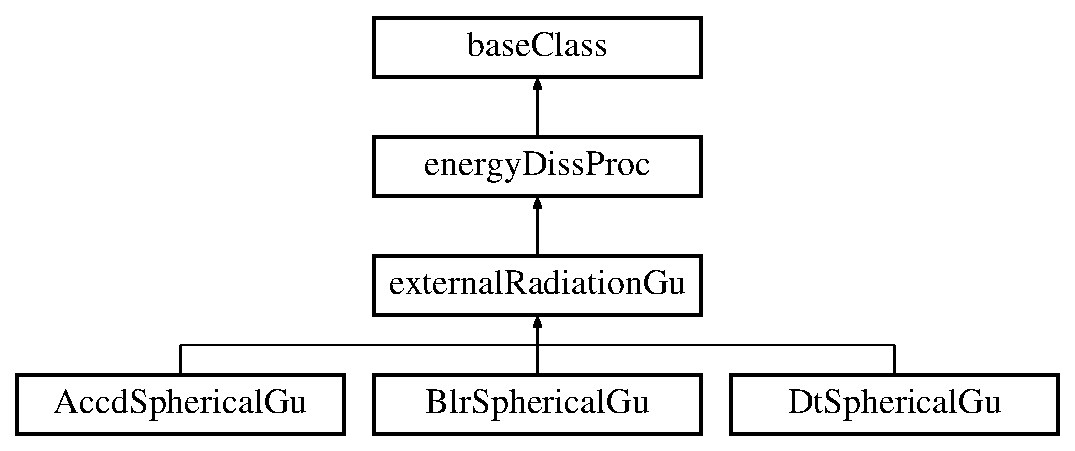
\includegraphics[height=4.000000cm]{classexternalRadiationGu}
\end{center}
\end{figure}


\subsection{Detailed Description}
Class provides electron energy losses and luminosity calculation for inverse Compton process (E\-R\-C) for seed photons comming from B\-L\-R and H\-D\-R modelled as quasi-\/spherical sources with u\-\_\-ext modified by g\-\_\-u parameter \subsection*{Public Member Functions}
\begin{DoxyCompactItemize}
\item 
\hyperlink{classexternalRadiationGu_aad5903b642f08594be10d699cf9fb3b4}{external\-Radiation\-Gu} (scfgp $\ast$\-\_\-cfg, \hyperlink{classjetGeometry}{jet\-Geometry} $\ast$\-\_\-r, \hyperlink{classelectrons}{electrons} $\ast$\-\_\-ele, std\-::string \-\_\-id)
\item 
\hyperlink{classexternalRadiationGu_afdabb07f9855b4c34a48a5c1901ac467}{$\sim$external\-Radiation\-Gu} ()
\item 
virtual void \hyperlink{classexternalRadiationGu_a8aa28d939b0ecf2651f18cc4f5f6ba25}{print\-Info} ()
\item 
virtual void \hyperlink{classexternalRadiationGu_a730363f393f29aef9927e0bb84087116}{update} ()
\item 
virtual double \hyperlink{classexternalRadiationGu_ab7e1abcc40cf0538404e88a0febdfb02}{getvext} (double \-\_\-r)
\item 
virtual void \hyperlink{classexternalRadiationGu_a541b2bb7da733f10d83af6225b7ad5f8}{set\-Radius} ()
\item 
double \hyperlink{classexternalRadiationGu_a266fc022608ea384a80be8ad840d5957}{dotg} (double g)
\item 
double \hyperlink{classexternalRadiationGu_ab49dc8bf55384ec6acf09bc1732194a4}{calculate\-Lpv} (double v, double theta)
\item 
void \hyperlink{classexternalRadiationGu_a946369eee3485a821a5619c5ba310497}{set\-Lpv} ()
\end{DoxyCompactItemize}
\subsection*{Public Attributes}
\begin{DoxyCompactItemize}
\item 
\hypertarget{classexternalRadiationGu_af9d98a13908450ce5bcea27ea86742a2}{double {\bfseries Gamma}}\label{classexternalRadiationGu_af9d98a13908450ce5bcea27ea86742a2}

\item 
\hypertarget{classexternalRadiationGu_a4ab4f6256141c4f6de874ef5af2ebb50}{double {\bfseries theta\-Obs}}\label{classexternalRadiationGu_a4ab4f6256141c4f6de874ef5af2ebb50}

\item 
\hypertarget{classexternalRadiationGu_adb7e3a102fa102262a0d2eea3ca0b1fd}{double {\bfseries m\-B\-H}}\label{classexternalRadiationGu_adb7e3a102fa102262a0d2eea3ca0b1fd}

\item 
\hypertarget{classexternalRadiationGu_a77edc9892436318a992a39efb291520d}{double {\bfseries e\-Disk}}\label{classexternalRadiationGu_a77edc9892436318a992a39efb291520d}

\item 
\hypertarget{classexternalRadiationGu_a4352a5309f0dfbd2600f6dd82bb5bead}{double {\bfseries m\-Dot}}\label{classexternalRadiationGu_a4352a5309f0dfbd2600f6dd82bb5bead}

\item 
\hypertarget{classexternalRadiationGu_ac067f1d23e69bb9c3390f4161913e3fa}{int {\bfseries K\-N}}\label{classexternalRadiationGu_ac067f1d23e69bb9c3390f4161913e3fa}

\end{DoxyCompactItemize}


\subsection{Constructor \& Destructor Documentation}
\hypertarget{classexternalRadiationGu_aad5903b642f08594be10d699cf9fb3b4}{\index{external\-Radiation\-Gu@{external\-Radiation\-Gu}!external\-Radiation\-Gu@{external\-Radiation\-Gu}}
\index{external\-Radiation\-Gu@{external\-Radiation\-Gu}!externalRadiationGu@{external\-Radiation\-Gu}}
\subsubsection[{external\-Radiation\-Gu}]{\setlength{\rightskip}{0pt plus 5cm}external\-Radiation\-Gu\-::external\-Radiation\-Gu (
\begin{DoxyParamCaption}
\item[{scfgp $\ast$}]{\-\_\-cfg, }
\item[{{\bf jet\-Geometry} $\ast$}]{\-\_\-r, }
\item[{{\bf electrons} $\ast$}]{\-\_\-ele, }
\item[{std\-::string}]{\-\_\-id}
\end{DoxyParamCaption}
)}}\label{classexternalRadiationGu_aad5903b642f08594be10d699cf9fb3b4}
constructor 
\begin{DoxyParams}{Parameters}
{\em \-\_\-cfg} & -\/ scfgp class object \\
\hline
{\em \-\_\-r} & -\/ \hyperlink{classjetGeometry}{jet\-Geometry} class object \\
\hline
{\em \-\_\-ele} & -\/ electrons class object \\
\hline
{\em \-\_\-id} & \\
\hline
\end{DoxyParams}

\begin{DoxyCode}
9                                                                                                        : 
      \hyperlink{classenergyDissProc_a0cf0b423089016fbe8a697378c519590}{energyDissProc}( \_cfg, \_r, \_ele, \_id ) \{
10   \textcolor{comment}{/* requested parameters */}
11   \hyperlink{classbaseClass_a744f87a6ebe63da08256c022d42a4ca7}{cfg} -> request<int>(\textcolor{stringliteral}{"N"} + \hyperlink{classbaseClass_a4d5ff386a69bcbe21b5976f55b624df6}{id}, 200, &\hyperlink{classbaseClass_a2b4d07d2b46197d495de0477f4bb22f8}{N} );
12   \hyperlink{classbaseClass_a744f87a6ebe63da08256c022d42a4ca7}{cfg} -> request<double>(\textcolor{stringliteral}{"Gamma"}, 10.0, &Gamma );
13   \hyperlink{classbaseClass_a744f87a6ebe63da08256c022d42a4ca7}{cfg} -> request<double>(\textcolor{stringliteral}{"thetaObs"}, 0.1, &thetaObs );
14   \hyperlink{classbaseClass_a744f87a6ebe63da08256c022d42a4ca7}{cfg} -> request<int>(\textcolor{stringliteral}{"KN"}, 0, &KN );
15   \hyperlink{classbaseClass_a744f87a6ebe63da08256c022d42a4ca7}{cfg} -> request<double>(\textcolor{stringliteral}{"mBH"},1.0,&mBH);
16   \hyperlink{classbaseClass_a744f87a6ebe63da08256c022d42a4ca7}{cfg} -> request<double>(\textcolor{stringliteral}{"eDisk"},0.1,&eDisk);
17   \hyperlink{classbaseClass_a744f87a6ebe63da08256c022d42a4ca7}{cfg} -> request<double>(\textcolor{stringliteral}{"mDot"},1.0,&mDot);
18   \hyperlink{classbaseClass_a744f87a6ebe63da08256c022d42a4ca7}{cfg} -> request<int>(\textcolor{keywordtype}{id}+\textcolor{stringliteral}{"LuminosityConstU"},0,&\hyperlink{classenergyDissProc_a2cc4e4eae15982f977a0dfa5458d80f4}{luminosityConstU});  
19   \hyperlink{classbaseClass_a744f87a6ebe63da08256c022d42a4ca7}{cfg} -> request<int>(\textcolor{keywordtype}{id}+\textcolor{stringliteral}{"LuminosityConstNu"},0,&\hyperlink{classenergyDissProc_a0a23854c1c830dfb9ac33d116fce5b7d}{luminosityConstNu});  
20 
21   \hyperlink{classbaseClass_a744f87a6ebe63da08256c022d42a4ca7}{cfg} -> updateRequests( ); \}
\end{DoxyCode}
\hypertarget{classexternalRadiationGu_afdabb07f9855b4c34a48a5c1901ac467}{\index{external\-Radiation\-Gu@{external\-Radiation\-Gu}!$\sim$external\-Radiation\-Gu@{$\sim$external\-Radiation\-Gu}}
\index{$\sim$external\-Radiation\-Gu@{$\sim$external\-Radiation\-Gu}!externalRadiationGu@{external\-Radiation\-Gu}}
\subsubsection[{$\sim$external\-Radiation\-Gu}]{\setlength{\rightskip}{0pt plus 5cm}external\-Radiation\-Gu\-::$\sim$external\-Radiation\-Gu (
\begin{DoxyParamCaption}
{}
\end{DoxyParamCaption}
)}}\label{classexternalRadiationGu_afdabb07f9855b4c34a48a5c1901ac467}
destructor 
\begin{DoxyCode}
23                                            \{
24   freeLpv( );
25   freeLvPoint( );
26   freeLvPointAvg( );
27   freeUpeR( ); \}
\end{DoxyCode}


\subsection{Member Function Documentation}
\hypertarget{classexternalRadiationGu_ab49dc8bf55384ec6acf09bc1732194a4}{\index{external\-Radiation\-Gu@{external\-Radiation\-Gu}!calculate\-Lpv@{calculate\-Lpv}}
\index{calculate\-Lpv@{calculate\-Lpv}!externalRadiationGu@{external\-Radiation\-Gu}}
\subsubsection[{calculate\-Lpv}]{\setlength{\rightskip}{0pt plus 5cm}double external\-Radiation\-Gu\-::calculate\-Lpv (
\begin{DoxyParamCaption}
\item[{double}]{v, }
\item[{double}]{theta}
\end{DoxyParamCaption}
)}}\label{classexternalRadiationGu_ab49dc8bf55384ec6acf09bc1732194a4}
calculate intrinsic luminosity 
\begin{DoxyParams}{Parameters}
{\em v} & -\/ frequency (jet co-\/moving frame) \\
\hline
\end{DoxyParams}
\begin{DoxyReturn}{Returns}
L'\-\_\-v 
\end{DoxyReturn}

\begin{DoxyCode}
36                                                                  \{
37   \textcolor{keywordtype}{double} Int = 0.0;
38   \textcolor{keywordtype}{double} e, miu, \hyperlink{classenergyDissProc_a36330825cd7737639d5d223281b1c7e1}{ep};
39 
40   e = PLANCK\_H*v/mec2;
41   miu = -( cos(theta)-\hyperlink{classbaseClass_a208facecf3a4480b47bebfce91413a39}{beta}(Gamma) )/( 1.0-\hyperlink{classbaseClass_a208facecf3a4480b47bebfce91413a39}{beta}(Gamma)*cos(theta) );
42   ep = \hyperlink{classexternalRadiationGu_ab7e1abcc40cf0538404e88a0febdfb02}{getvext}( \hyperlink{classbaseClass_a482bb9b1d94f3eb3f31026d14e9a2bb6}{r}->get() )*PLANCK\_H*Gamma/mec2;
43 
44   \textcolor{keywordflow}{for}( \textcolor{keywordtype}{int} k=0;k<\hyperlink{classenergyDissProc_a0dbf0777938131e938c1fdad5df38a7f}{ele}->\hyperlink{classbaseClass_a6ba5c4ce24742db73f45064337cf6963}{getN}( );k++ )
45     Int  += bazinga::IntCor( k, \hyperlink{classenergyDissProc_a0dbf0777938131e938c1fdad5df38a7f}{ele}->\hyperlink{classbaseClass_a6ba5c4ce24742db73f45064337cf6963}{getN}( ) )*inverseCompton::f( \hyperlink{classenergyDissProc_a0dbf0777938131e938c1fdad5df38a7f}{ele}->
      \hyperlink{classelectrons_afb0d9365f13787f44d23fb489732fc90}{getGamma}(k), \hyperlink{classenergyDissProc_a36330825cd7737639d5d223281b1c7e1}{ep}, e, miu )*\hyperlink{classenergyDissProc_a0dbf0777938131e938c1fdad5df38a7f}{ele}->\hyperlink{classelectrons_a24fbbed0acac968ce6b2ef2c5043dee4}{getNgamma}(k)/\hyperlink{classenergyDissProc_a0dbf0777938131e938c1fdad5df38a7f}{ele}->
      \hyperlink{classelectrons_afb0d9365f13787f44d23fb489732fc90}{getGamma}(k);
46 
47   \textcolor{keywordflow}{if}( \hyperlink{classenergyDissProc_a2cc4e4eae15982f977a0dfa5458d80f4}{luminosityConstU} )
48     \{ Int *= gsl\_vector\_get( \hyperlink{classenergyDissProc_ac925d66519c79f36421f75a6bc9f0965}{upe\_r}, 0 )*\hyperlink{classenergyDissProc_a0dbf0777938131e938c1fdad5df38a7f}{ele}->\hyperlink{classelectrons_a4e3d4179ce211bd732580b49914874e6}{getdLogGamma}( )/pow( 
      \hyperlink{classexternalRadiationGu_ab7e1abcc40cf0538404e88a0febdfb02}{getvext}( \hyperlink{classbaseClass_a482bb9b1d94f3eb3f31026d14e9a2bb6}{r}->get() ), 2.0 ); \}
49   \textcolor{keywordflow}{else} 
50     \{ Int *= gsl\_vector\_get( \hyperlink{classenergyDissProc_ac925d66519c79f36421f75a6bc9f0965}{upe\_r}, \hyperlink{classbaseClass_a482bb9b1d94f3eb3f31026d14e9a2bb6}{r}->getIndex( ) )*\hyperlink{classenergyDissProc_a0dbf0777938131e938c1fdad5df38a7f}{ele}->\hyperlink{classelectrons_a4e3d4179ce211bd732580b49914874e6}{getdLogGamma}( )/pow( 
      \hyperlink{classexternalRadiationGu_ab7e1abcc40cf0538404e88a0febdfb02}{getvext}( \hyperlink{classbaseClass_a482bb9b1d94f3eb3f31026d14e9a2bb6}{r}->get( ) ), 2.0 ); \}
51 
52   Int *= (3.0*SIGMA\_T*LIGHT\_SPEED)/(4.0*pow(Gamma,2.0));
53   Int *= v;
54   \textcolor{keywordflow}{return} Int; \}
\end{DoxyCode}
\hypertarget{classexternalRadiationGu_a266fc022608ea384a80be8ad840d5957}{\index{external\-Radiation\-Gu@{external\-Radiation\-Gu}!dotg@{dotg}}
\index{dotg@{dotg}!externalRadiationGu@{external\-Radiation\-Gu}}
\subsubsection[{dotg}]{\setlength{\rightskip}{0pt plus 5cm}double external\-Radiation\-Gu\-::dotg (
\begin{DoxyParamCaption}
\item[{double}]{g}
\end{DoxyParamCaption}
)\hspace{0.3cm}{\ttfamily [virtual]}}}\label{classexternalRadiationGu_a266fc022608ea384a80be8ad840d5957}
get d gamma \textbackslash{} d t for particular process 
\begin{DoxyParams}{Parameters}
{\em g} & -\/ electron Lorentz factor \\
\hline
\end{DoxyParams}
\begin{DoxyReturn}{Returns}
d gamma \textbackslash{} d t 
\end{DoxyReturn}


Reimplemented from \hyperlink{classenergyDissProc_a8074e0db5d859a8815e7136c2fc41b46}{energy\-Diss\-Proc}.


\begin{DoxyCode}
29                                            \{
30   \textcolor{keywordtype}{double} b, val = 0.0;
31   b = 4.0*g*\hyperlink{classexternalRadiationGu_ab7e1abcc40cf0538404e88a0febdfb02}{getvext}( \hyperlink{classbaseClass_a482bb9b1d94f3eb3f31026d14e9a2bb6}{r}->get() )*PLANCK\_H*Gamma/mec2;
32   \textcolor{keywordflow}{if}( b > 1.0 ) \{ \hyperlink{classenergyDissProc_a69ea4be814273e47e69e31e593c3a250}{set\_KN\_info}( g ); \}
33   val = gsl\_vector\_get( \hyperlink{classenergyDissProc_ac925d66519c79f36421f75a6bc9f0965}{upe\_r}, \hyperlink{classbaseClass_a482bb9b1d94f3eb3f31026d14e9a2bb6}{r}->getIndex( ) )*inverseCompton::fKN(b,KN); 
34   \textcolor{keywordflow}{return} val; \}
\end{DoxyCode}
\hypertarget{classexternalRadiationGu_ab7e1abcc40cf0538404e88a0febdfb02}{\index{external\-Radiation\-Gu@{external\-Radiation\-Gu}!getvext@{getvext}}
\index{getvext@{getvext}!externalRadiationGu@{external\-Radiation\-Gu}}
\subsubsection[{getvext}]{\setlength{\rightskip}{0pt plus 5cm}virtual double external\-Radiation\-Gu\-::getvext (
\begin{DoxyParamCaption}
\item[{double}]{\-\_\-r}
\end{DoxyParamCaption}
)\hspace{0.3cm}{\ttfamily [inline]}, {\ttfamily [virtual]}}}\label{classexternalRadiationGu_ab7e1abcc40cf0538404e88a0febdfb02}
get v\-\_\-ext value in Hz 
\begin{DoxyParams}{Parameters}
{\em \-\_\-r} & -\/ radius \\
\hline
\end{DoxyParams}
\begin{DoxyReturn}{Returns}
v\-\_\-ext 
\end{DoxyReturn}


Reimplemented in \hyperlink{classBlrSphericalGu_a78d8a3ace3f41082c48df04ea01bc142}{Blr\-Spherical\-Gu}, \hyperlink{classDtSphericalGu_a78218d880e1c9374058b6084ca939804}{Dt\-Spherical\-Gu}, and \hyperlink{classAccdSphericalGu_a802ac0782b844446953d4b59da160e46}{Accd\-Spherical\-Gu}.


\begin{DoxyCode}
46 \{ \}
\end{DoxyCode}
\hypertarget{classexternalRadiationGu_a8aa28d939b0ecf2651f18cc4f5f6ba25}{\index{external\-Radiation\-Gu@{external\-Radiation\-Gu}!print\-Info@{print\-Info}}
\index{print\-Info@{print\-Info}!externalRadiationGu@{external\-Radiation\-Gu}}
\subsubsection[{print\-Info}]{\setlength{\rightskip}{0pt plus 5cm}virtual void external\-Radiation\-Gu\-::print\-Info (
\begin{DoxyParamCaption}
{}
\end{DoxyParamCaption}
)\hspace{0.3cm}{\ttfamily [inline]}, {\ttfamily [virtual]}}}\label{classexternalRadiationGu_a8aa28d939b0ecf2651f18cc4f5f6ba25}
print basic information about myself (virtual) 

Reimplemented from \hyperlink{classenergyDissProc_ad1fbde0f7635a19a81412b9766916eb9}{energy\-Diss\-Proc}.



Reimplemented in \hyperlink{classBlrSphericalGu_a69de552417b7b01c3634650aaa9413d7}{Blr\-Spherical\-Gu}, \hyperlink{classDtSphericalGu_aeed0bda6440570b686aaf85bf5d2b6b3}{Dt\-Spherical\-Gu}, and \hyperlink{classAccdSphericalGu_a672f673606422556c3fb31a1787c6724}{Accd\-Spherical\-Gu}.


\begin{DoxyCode}
38 \{ \}
\end{DoxyCode}
\hypertarget{classexternalRadiationGu_a946369eee3485a821a5619c5ba310497}{\index{external\-Radiation\-Gu@{external\-Radiation\-Gu}!set\-Lpv@{set\-Lpv}}
\index{set\-Lpv@{set\-Lpv}!externalRadiationGu@{external\-Radiation\-Gu}}
\subsubsection[{set\-Lpv}]{\setlength{\rightskip}{0pt plus 5cm}void external\-Radiation\-Gu\-::set\-Lpv (
\begin{DoxyParamCaption}
{}
\end{DoxyParamCaption}
)\hspace{0.3cm}{\ttfamily [virtual]}}}\label{classexternalRadiationGu_a946369eee3485a821a5619c5ba310497}
set intrinsic luminosities 

Reimplemented from \hyperlink{classenergyDissProc_a93a39df53f30801f9f057cd55c05485d}{energy\-Diss\-Proc}.


\begin{DoxyCode}
56                                   \{
57   \textcolor{keywordflow}{for}( \textcolor{keywordtype}{int} i=0;i<\hyperlink{classbaseClass_a2b4d07d2b46197d495de0477f4bb22f8}{N};i++ ) \{ set\_Lpv( i, \hyperlink{classexternalRadiationGu_ab49dc8bf55384ec6acf09bc1732194a4}{calculateLpv}( get\_vp(i),thetaObs ) ); \}
58 \}
\end{DoxyCode}
\hypertarget{classexternalRadiationGu_a541b2bb7da733f10d83af6225b7ad5f8}{\index{external\-Radiation\-Gu@{external\-Radiation\-Gu}!set\-Radius@{set\-Radius}}
\index{set\-Radius@{set\-Radius}!externalRadiationGu@{external\-Radiation\-Gu}}
\subsubsection[{set\-Radius}]{\setlength{\rightskip}{0pt plus 5cm}virtual void external\-Radiation\-Gu\-::set\-Radius (
\begin{DoxyParamCaption}
{}
\end{DoxyParamCaption}
)\hspace{0.3cm}{\ttfamily [inline]}, {\ttfamily [virtual]}}}\label{classexternalRadiationGu_a541b2bb7da733f10d83af6225b7ad5f8}
set radial boundaries for processes 

Reimplemented in \hyperlink{classBlrSphericalGu_a51161abb05542e2120756bbdba82fc0b}{Blr\-Spherical\-Gu}, \hyperlink{classDtSphericalGu_af8b00665c5f7caca8b4a84034a097e05}{Dt\-Spherical\-Gu}, and \hyperlink{classAccdSphericalGu_a606c270f0d33338544b48373fe294f6b}{Accd\-Spherical\-Gu}.


\begin{DoxyCode}
49 \{ \}
\end{DoxyCode}
\hypertarget{classexternalRadiationGu_a730363f393f29aef9927e0bb84087116}{\index{external\-Radiation\-Gu@{external\-Radiation\-Gu}!update@{update}}
\index{update@{update}!externalRadiationGu@{external\-Radiation\-Gu}}
\subsubsection[{update}]{\setlength{\rightskip}{0pt plus 5cm}virtual void external\-Radiation\-Gu\-::update (
\begin{DoxyParamCaption}
{}
\end{DoxyParamCaption}
)\hspace{0.3cm}{\ttfamily [inline]}, {\ttfamily [virtual]}}}\label{classexternalRadiationGu_a730363f393f29aef9927e0bb84087116}
calculate and set Upe every time with new radius r 

Reimplemented from \hyperlink{classenergyDissProc_a6033524ea3d0fe38056bd74622f6c4ad}{energy\-Diss\-Proc}.



Reimplemented in \hyperlink{classBlrSphericalGu_a0054a1bc21351e6d68b8b5190ab1a8b0}{Blr\-Spherical\-Gu}, \hyperlink{classDtSphericalGu_ac940befec9ea9886b136f9d96c88620a}{Dt\-Spherical\-Gu}, and \hyperlink{classAccdSphericalGu_a278cae9b07c99dd7398121a77fa069c9}{Accd\-Spherical\-Gu}.


\begin{DoxyCode}
41 \{ \}
\end{DoxyCode}


The documentation for this class was generated from the following files\-:\begin{DoxyCompactItemize}
\item 
/home/mjaniak/\-Soft/blazar++/include/\hyperlink{externalRadiationGu_8hpp}{external\-Radiation\-Gu.\-hpp}\item 
/home/mjaniak/\-Soft/blazar++/src/\hyperlink{externalRadiationGu_8cpp}{external\-Radiation\-Gu.\-cpp}\end{DoxyCompactItemize}

\hypertarget{classexternalRadiationPlanar}{\section{external\-Radiation\-Planar Class Reference}
\label{classexternalRadiationPlanar}\index{external\-Radiation\-Planar@{external\-Radiation\-Planar}}
}


{\ttfamily \#include $<$external\-Radiation\-Planar.\-hpp$>$}

Inheritance diagram for external\-Radiation\-Planar\-:\begin{figure}[H]
\begin{center}
\leavevmode
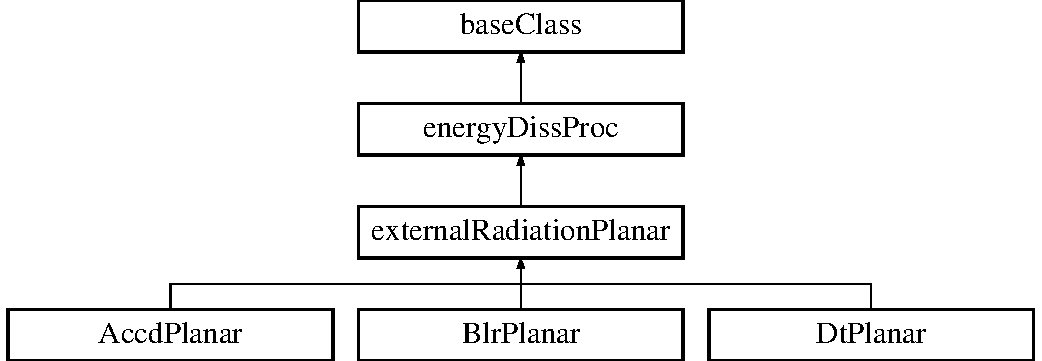
\includegraphics[height=4.000000cm]{classexternalRadiationPlanar}
\end{center}
\end{figure}


\subsection{Detailed Description}
Class provides electron energy losses and luminosity calculation for inverse Compton process (E\-R\-C) for seed photons comming from accretion disk, B\-L\-R and H\-D\-R modelled as planar source. Incoming photons are Doppler shifted depending on the geometry. Energy density of seed photons is calculated consistently based on the source characteristics in the accretion disk plane 
\begin{DoxyParams}{Parameters}
{\em alpha} & -\/ radiation vs R slope index \\
\hline
{\em R1} & -\/ inner edge \\
\hline
{\em R2} & -\/ outer edge \\
\hline
{\em s} & -\/ radiation vs R slope index \\
\hline
{\em approx} & -\/ approximation calculations switch \\
\hline
{\em fixed\-Upe} & -\/ fix u\-\_\-ext vs r \\
\hline
{\em save\-Rm} & -\/ switch to save information about R\-\_\-m \\
\hline
{\em R} & -\/ hirozontal disk plane radius \\
\hline
{\em rm} & -\/ R\-\_\-m vector info \\
\hline
{\em d\-Ld\-R} & -\/ vector to store information about d\-Ld\-R \\
\hline
\end{DoxyParams}
\subsection*{Public Member Functions}
\begin{DoxyCompactItemize}
\item 
\hyperlink{classexternalRadiationPlanar_a6254e3256914a093886b7af1f1dc4876}{external\-Radiation\-Planar} (scfgp $\ast$\-\_\-cfg, \hyperlink{classjetGeometry}{jet\-Geometry} $\ast$\-\_\-r, \hyperlink{classelectrons}{electrons} $\ast$\-\_\-ele, std\-::string \-\_\-id)
\item 
\hyperlink{classexternalRadiationPlanar_aab75f84c763bf0fb133ba3a3c5f0341c}{$\sim$external\-Radiation\-Planar} ()
\item 
virtual void \hyperlink{classexternalRadiationPlanar_a47e497b12dfa4e71311bffb3a4b384b2}{print\-Info} ()
\item 
virtual void \hyperlink{classexternalRadiationPlanar_a710859cda6258d75098ccb31e60ab261}{set\-Radius} ()
\item 
virtual double \hyperlink{classexternalRadiationPlanar_aa9ea7f37d1e43219f71ec6b215a38b96}{getvext} (double \-\_\-\-R)
\item 
virtual void \hyperlink{classexternalRadiationPlanar_a7914df2de2d822755ac1c9e6d860e22b}{setd\-Ld\-R} ()
\item 
void \hyperlink{classexternalRadiationPlanar_acfddae49394d11c89d1d47229ba8a3f7}{update} ()
\item 
double \hyperlink{classexternalRadiationPlanar_a14eca037d735b9cd1ad6d8f433052c62}{calculate\-Upe\-Full} ()
\item 
double \hyperlink{classexternalRadiationPlanar_a963d1270de3666c72509d5b1d405d72a}{calculate\-Upe\-Approx} (int index, bool flag)
\item 
double \hyperlink{classexternalRadiationPlanar_a90d75353e72674994f5a00d9de745f38}{function\-\_\-upe} (int index)
\item 
double \hyperlink{classexternalRadiationPlanar_a351a13f462898c59bae55ce606829648}{ctau} ()
\item 
double \hyperlink{classexternalRadiationPlanar_a7facfb7bbb0dfa8586ec30ae6d293aab}{getd\-Ld\-R} (int index)
\item 
double \hyperlink{classexternalRadiationPlanar_a4f49eec94e9d935df18534fe021c750c}{dotg} (double g)
\item 
void \hyperlink{classexternalRadiationPlanar_a8023104635baec445f038e9f1ca6c3bc}{set\-Lpv} ()
\item 
double \hyperlink{classexternalRadiationPlanar_a82753cf790d39965e72c07818a1bfa5e}{calculate\-Lpv} (double v, double theta)
\item 
double \hyperlink{classexternalRadiationPlanar_aaebb696a7bc742d22f9f8aadbcb4faaf}{fsc\-\_\-integral} (double v, double theta, double R)
\item 
double \hyperlink{classexternalRadiationPlanar_ab8c43b04bfea46ca0bc5e122ee12cc32}{function\-\_\-lum} (int index, double v, double theta)
\item 
\hypertarget{classexternalRadiationPlanar_aacba4508f03b16a8b19246cb6cb41eaa}{void {\bfseries allocate\-Rm} ()}\label{classexternalRadiationPlanar_aacba4508f03b16a8b19246cb6cb41eaa}

\item 
\hypertarget{classexternalRadiationPlanar_a6a42790e6070c19e8808a5527830727f}{void {\bfseries allocated\-Ld\-R} ()}\label{classexternalRadiationPlanar_a6a42790e6070c19e8808a5527830727f}

\item 
\hypertarget{classexternalRadiationPlanar_afce8fb037ad7ea93d3be175418186068}{void {\bfseries free\-Rm} ()}\label{classexternalRadiationPlanar_afce8fb037ad7ea93d3be175418186068}

\item 
double \hyperlink{classexternalRadiationPlanar_a3d9b58ccd4fcc4cdf50e583891897954}{get\-Rm} ()
\item 
void \hyperlink{classexternalRadiationPlanar_ad66a3f1f4fcc90ea0eeb40a9c3e1379a}{set\-Rm} (double val)
\item 
gsl\-\_\-vector $\ast$ \hyperlink{classexternalRadiationPlanar_a34bd0bdbb03089fce3f0a416dc4a4b72}{get\-Rm\-Vector} ()
\item 
void \hyperlink{classexternalRadiationPlanar_a1ca992aea51a737bf043a34c9f276055}{save\-Rm\-Vs\-R} ()
\end{DoxyCompactItemize}
\subsection*{Protected Attributes}
\begin{DoxyCompactItemize}
\item 
\hypertarget{classexternalRadiationPlanar_ad699086f216c0565e9246d86ef458a40}{double {\bfseries alpha}}\label{classexternalRadiationPlanar_ad699086f216c0565e9246d86ef458a40}

\item 
\hypertarget{classexternalRadiationPlanar_a20c946fc02d2cecf3f97278657a02044}{double {\bfseries R1}}\label{classexternalRadiationPlanar_a20c946fc02d2cecf3f97278657a02044}

\item 
\hypertarget{classexternalRadiationPlanar_a384b0f8bc9f8c57febeec6f4a86adcf7}{double {\bfseries R2}}\label{classexternalRadiationPlanar_a384b0f8bc9f8c57febeec6f4a86adcf7}

\item 
\hypertarget{classexternalRadiationPlanar_a2394ef823ede5bfb9222e3b73c001084}{double {\bfseries s}}\label{classexternalRadiationPlanar_a2394ef823ede5bfb9222e3b73c001084}

\item 
\hypertarget{classexternalRadiationPlanar_a77cc88ceca22b308e008cbd77c8b177e}{int {\bfseries approx}}\label{classexternalRadiationPlanar_a77cc88ceca22b308e008cbd77c8b177e}

\item 
\hypertarget{classexternalRadiationPlanar_a7446ecfda605a060bc0333cc460edbee}{double {\bfseries fixed\-Upe}}\label{classexternalRadiationPlanar_a7446ecfda605a060bc0333cc460edbee}

\item 
\hypertarget{classexternalRadiationPlanar_aa8f7460cdd0cc700fe6f1acd1f688a2f}{double {\bfseries Gamma}}\label{classexternalRadiationPlanar_aa8f7460cdd0cc700fe6f1acd1f688a2f}

\item 
\hypertarget{classexternalRadiationPlanar_a5036c94e73a39de03905eeb37a8043a8}{double {\bfseries theta\-Obs}}\label{classexternalRadiationPlanar_a5036c94e73a39de03905eeb37a8043a8}

\item 
\hypertarget{classexternalRadiationPlanar_ad25e39c6394ce3a08d7114f69b13990e}{int {\bfseries K\-N}}\label{classexternalRadiationPlanar_ad25e39c6394ce3a08d7114f69b13990e}

\item 
\hypertarget{classexternalRadiationPlanar_a04213265fbd5eca612b2709fea7cde25}{double {\bfseries m\-B\-H}}\label{classexternalRadiationPlanar_a04213265fbd5eca612b2709fea7cde25}

\item 
\hypertarget{classexternalRadiationPlanar_ac24e3609b5c2adec4382d05d0e75bb82}{double {\bfseries e\-Disk}}\label{classexternalRadiationPlanar_ac24e3609b5c2adec4382d05d0e75bb82}

\item 
\hypertarget{classexternalRadiationPlanar_a97e8ef6270b823ad876bbbcff29613ce}{double {\bfseries m\-Dot}}\label{classexternalRadiationPlanar_a97e8ef6270b823ad876bbbcff29613ce}

\item 
\hypertarget{classexternalRadiationPlanar_a6861b183760a624b958e1d53f098e858}{int {\bfseries save\-Rm}}\label{classexternalRadiationPlanar_a6861b183760a624b958e1d53f098e858}

\item 
\hypertarget{classexternalRadiationPlanar_a1dcd19343fa54db14337ac94cdb4cc1b}{\hyperlink{classlogGeometry}{log\-Geometry} $\ast$ {\bfseries R}}\label{classexternalRadiationPlanar_a1dcd19343fa54db14337ac94cdb4cc1b}

\item 
\hypertarget{classexternalRadiationPlanar_af6ba59b997f297ff1d7fd82942789a4d}{gsl\-\_\-vector $\ast$ {\bfseries rm}}\label{classexternalRadiationPlanar_af6ba59b997f297ff1d7fd82942789a4d}

\item 
\hypertarget{classexternalRadiationPlanar_a5382cffc8c19cf1d8128bc9808f16716}{gsl\-\_\-vector $\ast$ {\bfseries d\-Ld\-R}}\label{classexternalRadiationPlanar_a5382cffc8c19cf1d8128bc9808f16716}

\item 
\hypertarget{classexternalRadiationPlanar_af139b17f705a15a96de40d81a8904df1}{double {\bfseries Rm}}\label{classexternalRadiationPlanar_af139b17f705a15a96de40d81a8904df1}

\item 
\hypertarget{classexternalRadiationPlanar_a4bc11ce418aa033a86da524a5bba338d}{double {\bfseries Upe}}\label{classexternalRadiationPlanar_a4bc11ce418aa033a86da524a5bba338d}

\item 
\hypertarget{classexternalRadiationPlanar_acab7261d9c8a7f9dd0085171bcd4940c}{int {\bfseries Rm\-\_\-index}}\label{classexternalRadiationPlanar_acab7261d9c8a7f9dd0085171bcd4940c}

\end{DoxyCompactItemize}
\subsection*{Additional Inherited Members}


\subsection{Constructor \& Destructor Documentation}
\hypertarget{classexternalRadiationPlanar_a6254e3256914a093886b7af1f1dc4876}{\index{external\-Radiation\-Planar@{external\-Radiation\-Planar}!external\-Radiation\-Planar@{external\-Radiation\-Planar}}
\index{external\-Radiation\-Planar@{external\-Radiation\-Planar}!externalRadiationPlanar@{external\-Radiation\-Planar}}
\subsubsection[{external\-Radiation\-Planar}]{\setlength{\rightskip}{0pt plus 5cm}external\-Radiation\-Planar\-::external\-Radiation\-Planar (
\begin{DoxyParamCaption}
\item[{scfgp $\ast$}]{\-\_\-cfg, }
\item[{{\bf jet\-Geometry} $\ast$}]{\-\_\-r, }
\item[{{\bf electrons} $\ast$}]{\-\_\-ele, }
\item[{std\-::string}]{\-\_\-id}
\end{DoxyParamCaption}
)}}\label{classexternalRadiationPlanar_a6254e3256914a093886b7af1f1dc4876}
constructor 
\begin{DoxyParams}{Parameters}
{\em \-\_\-cfg} & -\/ scfgp class object \\
\hline
{\em \-\_\-r} & -\/ \hyperlink{classjetGeometry}{jet\-Geometry} class object \\
\hline
{\em \-\_\-ele} & -\/ electrons class object \\
\hline
{\em \-\_\-id} & \\
\hline
\end{DoxyParams}

\begin{DoxyCode}
9                                                                                                            
          : \hyperlink{classenergyDissProc_a0cf0b423089016fbe8a697378c519590}{energyDissProc}( \_cfg, \_r, \_ele, \_id ) \{
10   \textcolor{comment}{/* requested parameters */}
11   \textcolor{comment}{/* R1, R2, s, alpha - needed by Accd, BlrPl, DtPl */}
12   \hyperlink{classbaseClass_a744f87a6ebe63da08256c022d42a4ca7}{cfg} -> request<int>(\textcolor{stringliteral}{"N"} + \hyperlink{classbaseClass_a4d5ff386a69bcbe21b5976f55b624df6}{id}, 200, &\hyperlink{classbaseClass_a2b4d07d2b46197d495de0477f4bb22f8}{N} );
13   \hyperlink{classbaseClass_a744f87a6ebe63da08256c022d42a4ca7}{cfg} -> request<double>(\textcolor{keywordtype}{id} +  \textcolor{stringliteral}{"R1"}, 0.0, &R1 );
14   \hyperlink{classbaseClass_a744f87a6ebe63da08256c022d42a4ca7}{cfg} -> request<double>(\textcolor{keywordtype}{id} +  \textcolor{stringliteral}{"R2"}, 0.0, &R2 );
15   \hyperlink{classbaseClass_a744f87a6ebe63da08256c022d42a4ca7}{cfg} -> request<double>(\textcolor{keywordtype}{id} +  \textcolor{stringliteral}{"s"}, 0.0, &s );
16   \hyperlink{classbaseClass_a744f87a6ebe63da08256c022d42a4ca7}{cfg} -> request<double>(\textcolor{keywordtype}{id} +  \textcolor{stringliteral}{"alpha"}, 0.0, &alpha );
17   \hyperlink{classbaseClass_a744f87a6ebe63da08256c022d42a4ca7}{cfg} -> request<double>(\textcolor{stringliteral}{"Gamma"}, 10.0, &Gamma );
18   \hyperlink{classbaseClass_a744f87a6ebe63da08256c022d42a4ca7}{cfg} -> request<double>(\textcolor{stringliteral}{"thetaObs"}, 0.1, &thetaObs );
19   \hyperlink{classbaseClass_a744f87a6ebe63da08256c022d42a4ca7}{cfg} -> request<int>(\textcolor{stringliteral}{"KN"}, 0, &KN );
20   \hyperlink{classbaseClass_a744f87a6ebe63da08256c022d42a4ca7}{cfg} -> request<double>(\textcolor{stringliteral}{"mBH"},1.0,&mBH);
21   \hyperlink{classbaseClass_a744f87a6ebe63da08256c022d42a4ca7}{cfg} -> request<double>(\textcolor{stringliteral}{"eDisk"},0.1,&eDisk);
22   \hyperlink{classbaseClass_a744f87a6ebe63da08256c022d42a4ca7}{cfg} -> request<double>(\textcolor{stringliteral}{"mDot"},1.0,&mDot);
23   \hyperlink{classbaseClass_a744f87a6ebe63da08256c022d42a4ca7}{cfg} -> request<int>(\textcolor{keywordtype}{id}+\textcolor{stringliteral}{"LuminosityConstU"},0,&\hyperlink{classenergyDissProc_a2cc4e4eae15982f977a0dfa5458d80f4}{luminosityConstU});  
24   \hyperlink{classbaseClass_a744f87a6ebe63da08256c022d42a4ca7}{cfg} -> request<int>(\textcolor{keywordtype}{id}+\textcolor{stringliteral}{"LuminosityConstNu"},0,&\hyperlink{classenergyDissProc_a0a23854c1c830dfb9ac33d116fce5b7d}{luminosityConstNu});  
25 
26   \textcolor{comment}{/* works for both stratifications and for Accd */}
27   \hyperlink{classbaseClass_a744f87a6ebe63da08256c022d42a4ca7}{cfg} -> request<int>(\textcolor{stringliteral}{"extPlApp"},0,&approx);
28   \hyperlink{classbaseClass_a744f87a6ebe63da08256c022d42a4ca7}{cfg} -> request<int>(\textcolor{stringliteral}{"saveRmVsR"},0,&saveRm);
29   
30   \hyperlink{classbaseClass_a744f87a6ebe63da08256c022d42a4ca7}{cfg} -> updateRequests( );
31   
32   allocatedLdR( );
33   allocateRm( ); \}
\end{DoxyCode}
\hypertarget{classexternalRadiationPlanar_aab75f84c763bf0fb133ba3a3c5f0341c}{\index{external\-Radiation\-Planar@{external\-Radiation\-Planar}!$\sim$external\-Radiation\-Planar@{$\sim$external\-Radiation\-Planar}}
\index{$\sim$external\-Radiation\-Planar@{$\sim$external\-Radiation\-Planar}!externalRadiationPlanar@{external\-Radiation\-Planar}}
\subsubsection[{$\sim$external\-Radiation\-Planar}]{\setlength{\rightskip}{0pt plus 5cm}external\-Radiation\-Planar\-::$\sim$external\-Radiation\-Planar (
\begin{DoxyParamCaption}
{}
\end{DoxyParamCaption}
)}}\label{classexternalRadiationPlanar_aab75f84c763bf0fb133ba3a3c5f0341c}
destructor 
\begin{DoxyCode}
35                                                    \{
36   freeLpv( );
37   freeLvPoint( );
38   freeLvPointAvg( );
39   freeUpe( );
40   freeRm( );
41   
42   \textcolor{keyword}{delete} R;
43   R = NULL; \}
\end{DoxyCode}


\subsection{Member Function Documentation}
\hypertarget{classexternalRadiationPlanar_a82753cf790d39965e72c07818a1bfa5e}{\index{external\-Radiation\-Planar@{external\-Radiation\-Planar}!calculate\-Lpv@{calculate\-Lpv}}
\index{calculate\-Lpv@{calculate\-Lpv}!externalRadiationPlanar@{external\-Radiation\-Planar}}
\subsubsection[{calculate\-Lpv}]{\setlength{\rightskip}{0pt plus 5cm}double external\-Radiation\-Planar\-::calculate\-Lpv (
\begin{DoxyParamCaption}
\item[{double}]{v, }
\item[{double}]{theta}
\end{DoxyParamCaption}
)}}\label{classexternalRadiationPlanar_a82753cf790d39965e72c07818a1bfa5e}
calculate intrinsic luminosity 
\begin{DoxyParams}{Parameters}
{\em v} & -\/ frequency (jet co-\/moving frame) \\
\hline
\end{DoxyParams}
\begin{DoxyReturn}{Returns}
L'\-\_\-v 
\end{DoxyReturn}

\begin{DoxyCode}
152                                                                      \{
153   \textcolor{keywordtype}{double} val = 0.0;
154   \textcolor{keywordflow}{if}( approx ) \{ val = \hyperlink{classexternalRadiationPlanar_ab8c43b04bfea46ca0bc5e122ee12cc32}{function\_lum}( Rm\_index, v, theta )*Rm; \}
155   \textcolor{keywordflow}{else} \{
156     \textcolor{keywordflow}{for}( \textcolor{keywordtype}{int} i=0;i<R->getMaxIndex();i++ ) \{
157       R -> \hyperlink{classexternalRadiationPlanar_acfddae49394d11c89d1d47229ba8a3f7}{update}( i );
158       val += bazinga::IntCor( i, R->getN( ) )*\hyperlink{classexternalRadiationPlanar_ab8c43b04bfea46ca0bc5e122ee12cc32}{function\_lum}( i, v, theta )*R->getDr(i); \}
159   \}
160 
161   val *= 3.0*SIGMA\_T/(16.0*M\_PI);
162   val *= v;
163   \textcolor{keywordflow}{return} val; \}
\end{DoxyCode}
\hypertarget{classexternalRadiationPlanar_a963d1270de3666c72509d5b1d405d72a}{\index{external\-Radiation\-Planar@{external\-Radiation\-Planar}!calculate\-Upe\-Approx@{calculate\-Upe\-Approx}}
\index{calculate\-Upe\-Approx@{calculate\-Upe\-Approx}!externalRadiationPlanar@{external\-Radiation\-Planar}}
\subsubsection[{calculate\-Upe\-Approx}]{\setlength{\rightskip}{0pt plus 5cm}double external\-Radiation\-Planar\-::calculate\-Upe\-Approx (
\begin{DoxyParamCaption}
\item[{int}]{index, }
\item[{bool}]{flag}
\end{DoxyParamCaption}
)}}\label{classexternalRadiationPlanar_a963d1270de3666c72509d5b1d405d72a}
caculate u'\-\_\-ext in the jet co-\/moving frame using approximate equations 
\begin{DoxyParams}{Parameters}
{\em i} & -\/ index in radius R at which u'\-\_\-ext is calculated \\
\hline
{\em flag} & -\/ obsolete ? \\
\hline
\end{DoxyParams}
\begin{DoxyReturn}{Returns}
u'\-\_\-ext 
\end{DoxyReturn}

\begin{DoxyCode}
89 \{ \textcolor{keywordflow}{return} \hyperlink{classexternalRadiationPlanar_a90d75353e72674994f5a00d9de745f38}{function\_upe}( index )*R->get(index); \}
\end{DoxyCode}
\hypertarget{classexternalRadiationPlanar_a14eca037d735b9cd1ad6d8f433052c62}{\index{external\-Radiation\-Planar@{external\-Radiation\-Planar}!calculate\-Upe\-Full@{calculate\-Upe\-Full}}
\index{calculate\-Upe\-Full@{calculate\-Upe\-Full}!externalRadiationPlanar@{external\-Radiation\-Planar}}
\subsubsection[{calculate\-Upe\-Full}]{\setlength{\rightskip}{0pt plus 5cm}double external\-Radiation\-Planar\-::calculate\-Upe\-Full (
\begin{DoxyParamCaption}
{}
\end{DoxyParamCaption}
)}}\label{classexternalRadiationPlanar_a14eca037d735b9cd1ad6d8f433052c62}
caculate u'\-\_\-ext in the jet co-\/moving frame using full equations \begin{DoxyReturn}{Returns}
u'\-\_\-ext 
\end{DoxyReturn}

\begin{DoxyCode}
72                                                   \{
73   \textcolor{keywordtype}{double} \_Int = 0.0;
74   gsl\_vector *\_temp\_function\_upe\_vector = gsl\_vector\_alloc( \hyperlink{classbaseClass_a2b4d07d2b46197d495de0477f4bb22f8}{N} );
75   \textcolor{keywordtype}{double} \_function\_upe\_value = 0;
76 
77   \textcolor{keywordflow}{for}( \textcolor{keywordtype}{int} i=0;i<R->getMaxIndex();i++ ) \{
78     gsl\_vector\_set( \_temp\_function\_upe\_vector, i, \hyperlink{classexternalRadiationPlanar_a90d75353e72674994f5a00d9de745f38}{function\_upe}( i ) );
79     \_Int += bazinga::IntCor( i, R->getN( ) )*gsl\_vector\_get( \_temp\_function\_upe\_vector, i)*R->getDr(i);
80   \}
81   
82   \textcolor{comment}{/* before quit save \_temp\_function\_upe\_vector */}
83   bazinga::save\_GSLVector( \textcolor{stringliteral}{"dUpedR\_"}+this->\hyperlink{classbaseClass_a756d5accf10ced9a34024048c95a51c9}{whoAmI}( ), R->getRadius\_GSLVector( ), 
      \_temp\_function\_upe\_vector, R->getPosition( ), \hyperlink{classbaseClass_a744f87a6ebe63da08256c022d42a4ca7}{cfg}->get<std::string>(\textcolor{stringliteral}{"output"}) );
84   gsl\_vector\_free( \_temp\_function\_upe\_vector );
85   \_temp\_function\_upe\_vector = NULL;
86   
87   \textcolor{keywordflow}{return} \_Int; \}
\end{DoxyCode}
\hypertarget{classexternalRadiationPlanar_a351a13f462898c59bae55ce606829648}{\index{external\-Radiation\-Planar@{external\-Radiation\-Planar}!ctau@{ctau}}
\index{ctau@{ctau}!externalRadiationPlanar@{external\-Radiation\-Planar}}
\subsubsection[{ctau}]{\setlength{\rightskip}{0pt plus 5cm}double external\-Radiation\-Planar\-::ctau (
\begin{DoxyParamCaption}
{}
\end{DoxyParamCaption}
)}}\label{classexternalRadiationPlanar_a351a13f462898c59bae55ce606829648}
auxillary function to alculate u'\-\_\-ext -\/ normalization factor 
\begin{DoxyCode}
98                                       \{
99   \textcolor{keywordtype}{double} val = 0.0;
100   \textcolor{keywordflow}{if}( s == 1 ) \{ val = 1.0/log(R2/R1); \}
101   \textcolor{keywordflow}{else} \{ val = (1.0-s)/(pow(R2,1.0-s)-pow(R1,1.0-s)); \}
102   \textcolor{keywordflow}{return} val; \}
\end{DoxyCode}
\hypertarget{classexternalRadiationPlanar_a4f49eec94e9d935df18534fe021c750c}{\index{external\-Radiation\-Planar@{external\-Radiation\-Planar}!dotg@{dotg}}
\index{dotg@{dotg}!externalRadiationPlanar@{external\-Radiation\-Planar}}
\subsubsection[{dotg}]{\setlength{\rightskip}{0pt plus 5cm}double external\-Radiation\-Planar\-::dotg (
\begin{DoxyParamCaption}
\item[{double}]{g}
\end{DoxyParamCaption}
)\hspace{0.3cm}{\ttfamily [virtual]}}}\label{classexternalRadiationPlanar_a4f49eec94e9d935df18534fe021c750c}
get d gamma \textbackslash{} d t for particular process 
\begin{DoxyParams}{Parameters}
{\em g} & -\/ electron Lorentz factor \\
\hline
\end{DoxyParams}
\begin{DoxyReturn}{Returns}
d gamma \textbackslash{} d t 
\end{DoxyReturn}


Reimplemented from \hyperlink{classenergyDissProc_a8074e0db5d859a8815e7136c2fc41b46}{energy\-Diss\-Proc}.


\begin{DoxyCode}
106                                                \{
107   \textcolor{keywordtype}{double} val = 0.0;
108   \textcolor{keywordtype}{double} b = 0.0;
109   \textcolor{keywordtype}{double} r2R2 = pow(\hyperlink{classbaseClass_a482bb9b1d94f3eb3f31026d14e9a2bb6}{r}->get(),2.0)+pow(Rm,2.0);
110   
111   \textcolor{keywordtype}{double} doppler\_ext = 1.0/( Gamma*( 1.0-\hyperlink{classbaseClass_a208facecf3a4480b47bebfce91413a39}{beta}(Gamma)*(\hyperlink{classbaseClass_a482bb9b1d94f3eb3f31026d14e9a2bb6}{r}->get()/sqrt(r2R2)) ) );  
112   \textcolor{comment}{/* as e\_ext max we take e\_ext @ Rm where it is maximum; in case of BLRPL it makes no difference at all */}
113   b = 4.0*g*\hyperlink{classexternalRadiationPlanar_aa9ea7f37d1e43219f71ec6b215a38b96}{getvext}( Rm )*PLANCK\_H/(mec2*doppler\_ext);
114 
115   \textcolor{keywordflow}{if}( b > 1.0 ) \{ \hyperlink{classenergyDissProc_a69ea4be814273e47e69e31e593c3a250}{set\_KN\_info}( g ); \}
116   val = Upe*inverseCompton::FKN( b, alpha, KN ); \textcolor{comment}{/* fKN not used anymore; using FKN instead */}
117 
118   \textcolor{keywordflow}{return} val; \}
\end{DoxyCode}
\hypertarget{classexternalRadiationPlanar_aaebb696a7bc742d22f9f8aadbcb4faaf}{\index{external\-Radiation\-Planar@{external\-Radiation\-Planar}!fsc\-\_\-integral@{fsc\-\_\-integral}}
\index{fsc\-\_\-integral@{fsc\-\_\-integral}!externalRadiationPlanar@{external\-Radiation\-Planar}}
\subsubsection[{fsc\-\_\-integral}]{\setlength{\rightskip}{0pt plus 5cm}double external\-Radiation\-Planar\-::fsc\-\_\-integral (
\begin{DoxyParamCaption}
\item[{double}]{v, }
\item[{double}]{theta, }
\item[{double}]{R}
\end{DoxyParamCaption}
)}}\label{classexternalRadiationPlanar_aaebb696a7bc742d22f9f8aadbcb4faaf}
function that calculates intrinsic E\-R\-C luminosity 
\begin{DoxyParams}{Parameters}
{\em v} & -\/ frequency \\
\hline
{\em theta} & -\/ observer angle \\
\hline
{\em R} & -\/ radius in the accretion disk plane \\
\hline
\end{DoxyParams}
\begin{DoxyReturn}{Returns}
L' 
\end{DoxyReturn}

\begin{DoxyCode}
122                                                                                \{
123   \textcolor{keywordtype}{double} Int = 0.0;
124   \textcolor{keywordtype}{double} ee = PLANCK\_H*v/(ELECTRON\_MASS*LIGHT\_SPEED*LIGHT\_SPEED);
125   \textcolor{keywordtype}{double} miu = -(cos(theta)-\hyperlink{classbaseClass_a208facecf3a4480b47bebfce91413a39}{beta}(Gamma))/(1.0-\hyperlink{classbaseClass_a208facecf3a4480b47bebfce91413a39}{beta}(Gamma)*cos(theta));
126 
127   \textcolor{keywordtype}{double} r2R2, doppler\_ext;
128   \textcolor{keywordflow}{if}( \hyperlink{classenergyDissProc_a2cc4e4eae15982f977a0dfa5458d80f4}{luminosityConstU} ) \{
129     r2R2 = pow(\hyperlink{classbaseClass_a482bb9b1d94f3eb3f31026d14e9a2bb6}{r}->getRInjMax( ),2.0)+pow(R,2.0);
130     doppler\_ext = 1.0/( Gamma*( 1.0-\hyperlink{classbaseClass_a208facecf3a4480b47bebfce91413a39}{beta}(Gamma)*(\hyperlink{classbaseClass_a482bb9b1d94f3eb3f31026d14e9a2bb6}{r}->getRInjMax( )/sqrt(r2R2)) ) ); \}
131   \textcolor{keywordflow}{else} \{    
132     r2R2 = pow(\hyperlink{classbaseClass_a482bb9b1d94f3eb3f31026d14e9a2bb6}{r}->get(),2.0)+pow(R,2.0);
133     doppler\_ext = 1.0/( Gamma*( 1.0-\hyperlink{classbaseClass_a208facecf3a4480b47bebfce91413a39}{beta}(Gamma)*(\hyperlink{classbaseClass_a482bb9b1d94f3eb3f31026d14e9a2bb6}{r}->get()/sqrt(r2R2)) ) ); \}
134 
135   \textcolor{comment}{/* integration loop over electrons */}
136   \textcolor{keywordflow}{for}( \textcolor{keywordtype}{int} k=0;k<\hyperlink{classenergyDissProc_a0dbf0777938131e938c1fdad5df38a7f}{ele}->\hyperlink{classbaseClass_a6ba5c4ce24742db73f45064337cf6963}{getN}( );k++ ) \{ Int += bazinga::IntCor( k, \hyperlink{classenergyDissProc_a0dbf0777938131e938c1fdad5df38a7f}{ele}->
      \hyperlink{classbaseClass_a6ba5c4ce24742db73f45064337cf6963}{getN}( ) )*inverseCompton::f(\hyperlink{classenergyDissProc_a0dbf0777938131e938c1fdad5df38a7f}{ele}->\hyperlink{classelectrons_afb0d9365f13787f44d23fb489732fc90}{getGamma}(k), PLANCK\_H*\hyperlink{classexternalRadiationPlanar_aa9ea7f37d1e43219f71ec6b215a38b96}{getvext}( R )/(mec2*doppler\_ext
      ), ee, miu )*\hyperlink{classenergyDissProc_a0dbf0777938131e938c1fdad5df38a7f}{ele}->\hyperlink{classelectrons_a24fbbed0acac968ce6b2ef2c5043dee4}{getNgamma}(k)/\hyperlink{classenergyDissProc_a0dbf0777938131e938c1fdad5df38a7f}{ele}->\hyperlink{classelectrons_afb0d9365f13787f44d23fb489732fc90}{getGamma}(k); \}
137   
138   Int *= \hyperlink{classenergyDissProc_a0dbf0777938131e938c1fdad5df38a7f}{ele}->\hyperlink{classelectrons_a4e3d4179ce211bd732580b49914874e6}{getdLogGamma}( );
139   \textcolor{keywordflow}{return} Int; \}
\end{DoxyCode}
\hypertarget{classexternalRadiationPlanar_ab8c43b04bfea46ca0bc5e122ee12cc32}{\index{external\-Radiation\-Planar@{external\-Radiation\-Planar}!function\-\_\-lum@{function\-\_\-lum}}
\index{function\-\_\-lum@{function\-\_\-lum}!externalRadiationPlanar@{external\-Radiation\-Planar}}
\subsubsection[{function\-\_\-lum}]{\setlength{\rightskip}{0pt plus 5cm}double external\-Radiation\-Planar\-::function\-\_\-lum (
\begin{DoxyParamCaption}
\item[{int}]{index, }
\item[{double}]{v, }
\item[{double}]{theta}
\end{DoxyParamCaption}
)}}\label{classexternalRadiationPlanar_ab8c43b04bfea46ca0bc5e122ee12cc32}
auxillary function to calculate L' 
\begin{DoxyParams}{Parameters}
{\em index} & -\/ index in radius R at which L' is calculated \\
\hline
{\em v} & -\/ frequency \\
\hline
{\em theta} & -\/ observer angle \\
\hline
\end{DoxyParams}

\begin{DoxyCode}
141                                                                                 \{
142   \textcolor{keywordtype}{double} r2R2, doppler\_ext;
143   \textcolor{keywordflow}{if}( \hyperlink{classenergyDissProc_a2cc4e4eae15982f977a0dfa5458d80f4}{luminosityConstU} ) \{
144     r2R2 = pow(\hyperlink{classbaseClass_a482bb9b1d94f3eb3f31026d14e9a2bb6}{r}->getRInjMax( ),2.0)+pow(R->get(index),2.0);
145     doppler\_ext = 1.0/( Gamma*( 1.0-\hyperlink{classbaseClass_a208facecf3a4480b47bebfce91413a39}{beta}(Gamma)*(\hyperlink{classbaseClass_a482bb9b1d94f3eb3f31026d14e9a2bb6}{r}->getRInjMax( )/sqrt(r2R2)) ) ); \}
146   \textcolor{keywordflow}{else} \{    
147      r2R2 = pow(\hyperlink{classbaseClass_a482bb9b1d94f3eb3f31026d14e9a2bb6}{r}->get(),2.0)+pow(R->get(index),2.0);
148     doppler\_ext = 1.0/( Gamma*( 1.0-\hyperlink{classbaseClass_a208facecf3a4480b47bebfce91413a39}{beta}(Gamma)*(\hyperlink{classbaseClass_a482bb9b1d94f3eb3f31026d14e9a2bb6}{r}->get()/sqrt(r2R2)) ) ); \}
149 
150   \textcolor{keywordflow}{return} \hyperlink{classexternalRadiationPlanar_a7facfb7bbb0dfa8586ec30ae6d293aab}{getdLdR}(index)*\hyperlink{classexternalRadiationPlanar_aaebb696a7bc742d22f9f8aadbcb4faaf}{fsc\_integral}( v, theta, R->get(index) )/(r2R2*pow( 
      \hyperlink{classexternalRadiationPlanar_aa9ea7f37d1e43219f71ec6b215a38b96}{getvext}( R->get(index) ), 2 )); \}
\end{DoxyCode}
\hypertarget{classexternalRadiationPlanar_a90d75353e72674994f5a00d9de745f38}{\index{external\-Radiation\-Planar@{external\-Radiation\-Planar}!function\-\_\-upe@{function\-\_\-upe}}
\index{function\-\_\-upe@{function\-\_\-upe}!externalRadiationPlanar@{external\-Radiation\-Planar}}
\subsubsection[{function\-\_\-upe}]{\setlength{\rightskip}{0pt plus 5cm}double external\-Radiation\-Planar\-::function\-\_\-upe (
\begin{DoxyParamCaption}
\item[{int}]{index}
\end{DoxyParamCaption}
)}}\label{classexternalRadiationPlanar_a90d75353e72674994f5a00d9de745f38}
auxillary function to calculate u'\-\_\-ext 
\begin{DoxyParams}{Parameters}
{\em index} & -\/ index in radius R at which u'\-\_\-ext is calculated \\
\hline
\end{DoxyParams}

\begin{DoxyCode}
91                                                         \{
92   \textcolor{keywordtype}{double} val;
93   \textcolor{keywordtype}{double} r2R2 = pow(\hyperlink{classbaseClass_a482bb9b1d94f3eb3f31026d14e9a2bb6}{r}->get(),2.0)+pow(R->get(index),2);
94   val = \hyperlink{classexternalRadiationPlanar_a7facfb7bbb0dfa8586ec30ae6d293aab}{getdLdR}(index)*pow(1.0-((\hyperlink{classbaseClass_a208facecf3a4480b47bebfce91413a39}{beta}(Gamma)*\hyperlink{classbaseClass_a482bb9b1d94f3eb3f31026d14e9a2bb6}{r}->get())/sqrt(r2R2)),2)/r2R2;
95   val *= pow(Gamma,2)/(4.0*M\_PI*LIGHT\_SPEED);
96   \textcolor{keywordflow}{return} val; \}
\end{DoxyCode}
\hypertarget{classexternalRadiationPlanar_a7facfb7bbb0dfa8586ec30ae6d293aab}{\index{external\-Radiation\-Planar@{external\-Radiation\-Planar}!getd\-Ld\-R@{getd\-Ld\-R}}
\index{getd\-Ld\-R@{getd\-Ld\-R}!externalRadiationPlanar@{external\-Radiation\-Planar}}
\subsubsection[{getd\-Ld\-R}]{\setlength{\rightskip}{0pt plus 5cm}double external\-Radiation\-Planar\-::getd\-Ld\-R (
\begin{DoxyParamCaption}
\item[{int}]{index}
\end{DoxyParamCaption}
)}}\label{classexternalRadiationPlanar_a7facfb7bbb0dfa8586ec30ae6d293aab}
get fd\-Ld\-R 
\begin{DoxyParams}{Parameters}
{\em index} & in radius R at which d\-Ld\-R is calculated \\
\hline
\end{DoxyParams}

\begin{DoxyCode}
104 \{ \textcolor{keywordflow}{return} gsl\_vector\_get( dLdR, index ); \}
\end{DoxyCode}
\hypertarget{classexternalRadiationPlanar_a3d9b58ccd4fcc4cdf50e583891897954}{\index{external\-Radiation\-Planar@{external\-Radiation\-Planar}!get\-Rm@{get\-Rm}}
\index{get\-Rm@{get\-Rm}!externalRadiationPlanar@{external\-Radiation\-Planar}}
\subsubsection[{get\-Rm}]{\setlength{\rightskip}{0pt plus 5cm}double external\-Radiation\-Planar\-::get\-Rm (
\begin{DoxyParamCaption}
{}
\end{DoxyParamCaption}
)\hspace{0.3cm}{\ttfamily [inline]}}}\label{classexternalRadiationPlanar_a3d9b58ccd4fcc4cdf50e583891897954}
get R\-\_\-m -\/ radius at which contribution of u'\-\_\-ext is maximal \begin{DoxyReturn}{Returns}
R\-\_\-m 
\end{DoxyReturn}

\begin{DoxyCode}
126 \{ \textcolor{keywordflow}{return} gsl\_vector\_get( rm, \hyperlink{classbaseClass_a482bb9b1d94f3eb3f31026d14e9a2bb6}{r}->getIndex( ) ); \}
\end{DoxyCode}
\hypertarget{classexternalRadiationPlanar_a34bd0bdbb03089fce3f0a416dc4a4b72}{\index{external\-Radiation\-Planar@{external\-Radiation\-Planar}!get\-Rm\-Vector@{get\-Rm\-Vector}}
\index{get\-Rm\-Vector@{get\-Rm\-Vector}!externalRadiationPlanar@{external\-Radiation\-Planar}}
\subsubsection[{get\-Rm\-Vector}]{\setlength{\rightskip}{0pt plus 5cm}gsl\-\_\-vector$\ast$ external\-Radiation\-Planar\-::get\-Rm\-Vector (
\begin{DoxyParamCaption}
{}
\end{DoxyParamCaption}
)\hspace{0.3cm}{\ttfamily [inline]}}}\label{classexternalRadiationPlanar_a34bd0bdbb03089fce3f0a416dc4a4b72}
get vector with R\-\_\-m values stored 
\begin{DoxyCode}
134 \{ \textcolor{keywordflow}{return} rm; \}
\end{DoxyCode}
\hypertarget{classexternalRadiationPlanar_aa9ea7f37d1e43219f71ec6b215a38b96}{\index{external\-Radiation\-Planar@{external\-Radiation\-Planar}!getvext@{getvext}}
\index{getvext@{getvext}!externalRadiationPlanar@{external\-Radiation\-Planar}}
\subsubsection[{getvext}]{\setlength{\rightskip}{0pt plus 5cm}virtual double external\-Radiation\-Planar\-::getvext (
\begin{DoxyParamCaption}
\item[{double}]{\-\_\-\-R}
\end{DoxyParamCaption}
)\hspace{0.3cm}{\ttfamily [inline]}, {\ttfamily [virtual]}}}\label{classexternalRadiationPlanar_aa9ea7f37d1e43219f71ec6b215a38b96}
get v\-\_\-ext value in Hz 
\begin{DoxyParams}{Parameters}
{\em \-\_\-\-R} & -\/ radius in accretion disk plane \\
\hline
\end{DoxyParams}
\begin{DoxyReturn}{Returns}
v\-\_\-ext 
\end{DoxyReturn}


Reimplemented in \hyperlink{classBlrPlanar_abe8831b3b2d9ea5d632a354f1305bf86}{Blr\-Planar}, \hyperlink{classDtPlanar_a46eb0e18c9a391adccffe2623dd3dfbe}{Dt\-Planar}, and \hyperlink{classAccdPlanar_a1f9a8eadf2626c50ecf0a56d5b9a17de}{Accd\-Planar}.


\begin{DoxyCode}
68 \{ \textcolor{keywordflow}{return} 0; \}
\end{DoxyCode}
\hypertarget{classexternalRadiationPlanar_a47e497b12dfa4e71311bffb3a4b384b2}{\index{external\-Radiation\-Planar@{external\-Radiation\-Planar}!print\-Info@{print\-Info}}
\index{print\-Info@{print\-Info}!externalRadiationPlanar@{external\-Radiation\-Planar}}
\subsubsection[{print\-Info}]{\setlength{\rightskip}{0pt plus 5cm}virtual void external\-Radiation\-Planar\-::print\-Info (
\begin{DoxyParamCaption}
{}
\end{DoxyParamCaption}
)\hspace{0.3cm}{\ttfamily [inline]}, {\ttfamily [virtual]}}}\label{classexternalRadiationPlanar_a47e497b12dfa4e71311bffb3a4b384b2}
print basic information about myself (virtual) 

Reimplemented from \hyperlink{classenergyDissProc_ad1fbde0f7635a19a81412b9766916eb9}{energy\-Diss\-Proc}.



Reimplemented in \hyperlink{classBlrPlanar_a3321d83625869e16c5794d9419dff073}{Blr\-Planar}, \hyperlink{classDtPlanar_a0d1b6697d54a08030ed50b7e4b5fbfef}{Dt\-Planar}, and \hyperlink{classAccdPlanar_a51960bc05d15aedf068b65a369d1899c}{Accd\-Planar}.


\begin{DoxyCode}
60 \{ \}
\end{DoxyCode}
\hypertarget{classexternalRadiationPlanar_a1ca992aea51a737bf043a34c9f276055}{\index{external\-Radiation\-Planar@{external\-Radiation\-Planar}!save\-Rm\-Vs\-R@{save\-Rm\-Vs\-R}}
\index{save\-Rm\-Vs\-R@{save\-Rm\-Vs\-R}!externalRadiationPlanar@{external\-Radiation\-Planar}}
\subsubsection[{save\-Rm\-Vs\-R}]{\setlength{\rightskip}{0pt plus 5cm}void external\-Radiation\-Planar\-::save\-Rm\-Vs\-R (
\begin{DoxyParamCaption}
{}
\end{DoxyParamCaption}
)}}\label{classexternalRadiationPlanar_a1ca992aea51a737bf043a34c9f276055}
save vector with R\-\_\-m values stored 
\begin{DoxyCode}
175                                          \{
176  \textcolor{keywordflow}{if}( saveRm ) \{ bazinga::save\_GSLVector( \textcolor{stringliteral}{"Rm\_"}+ this->\hyperlink{classbaseClass_a756d5accf10ced9a34024048c95a51c9}{whoAmI}( ), \hyperlink{classbaseClass_a482bb9b1d94f3eb3f31026d14e9a2bb6}{r}->getRadius\_GSLVector( ), 
      \hyperlink{classexternalRadiationPlanar_a34bd0bdbb03089fce3f0a416dc4a4b72}{getRmVector}( ), \hyperlink{classbaseClass_a744f87a6ebe63da08256c022d42a4ca7}{cfg}->get<std::string>(\textcolor{stringliteral}{"output"}) ); \}
177 \}
\end{DoxyCode}
\hypertarget{classexternalRadiationPlanar_a7914df2de2d822755ac1c9e6d860e22b}{\index{external\-Radiation\-Planar@{external\-Radiation\-Planar}!setd\-Ld\-R@{setd\-Ld\-R}}
\index{setd\-Ld\-R@{setd\-Ld\-R}!externalRadiationPlanar@{external\-Radiation\-Planar}}
\subsubsection[{setd\-Ld\-R}]{\setlength{\rightskip}{0pt plus 5cm}virtual void external\-Radiation\-Planar\-::setd\-Ld\-R (
\begin{DoxyParamCaption}
{}
\end{DoxyParamCaption}
)\hspace{0.3cm}{\ttfamily [inline]}, {\ttfamily [virtual]}}}\label{classexternalRadiationPlanar_a7914df2de2d822755ac1c9e6d860e22b}
set d\-L/d\-R for particulat source 

Reimplemented in \hyperlink{classBlrPlanar_afcd6617d32754c8377b123317531b613}{Blr\-Planar}, \hyperlink{classDtPlanar_a6445269d74ae176c5d299ac71cd7ac87}{Dt\-Planar}, and \hyperlink{classAccdPlanar_ab4fdeb7f7898f380e2f9e333d430b2de}{Accd\-Planar}.


\begin{DoxyCode}
71 \{ \}
\end{DoxyCode}
\hypertarget{classexternalRadiationPlanar_a8023104635baec445f038e9f1ca6c3bc}{\index{external\-Radiation\-Planar@{external\-Radiation\-Planar}!set\-Lpv@{set\-Lpv}}
\index{set\-Lpv@{set\-Lpv}!externalRadiationPlanar@{external\-Radiation\-Planar}}
\subsubsection[{set\-Lpv}]{\setlength{\rightskip}{0pt plus 5cm}void external\-Radiation\-Planar\-::set\-Lpv (
\begin{DoxyParamCaption}
{}
\end{DoxyParamCaption}
)\hspace{0.3cm}{\ttfamily [virtual]}}}\label{classexternalRadiationPlanar_a8023104635baec445f038e9f1ca6c3bc}
set intrinsic luminosities 

Reimplemented from \hyperlink{classenergyDissProc_a93a39df53f30801f9f057cd55c05485d}{energy\-Diss\-Proc}.


\begin{DoxyCode}
120 \{ \textcolor{keywordflow}{for}( \textcolor{keywordtype}{int} i=0;i<\hyperlink{classbaseClass_a2b4d07d2b46197d495de0477f4bb22f8}{N};i++ ) set\_Lpv( i, \hyperlink{classexternalRadiationPlanar_a82753cf790d39965e72c07818a1bfa5e}{calculateLpv}( get\_vp(i), thetaObs )); \}
\end{DoxyCode}
\hypertarget{classexternalRadiationPlanar_a710859cda6258d75098ccb31e60ab261}{\index{external\-Radiation\-Planar@{external\-Radiation\-Planar}!set\-Radius@{set\-Radius}}
\index{set\-Radius@{set\-Radius}!externalRadiationPlanar@{external\-Radiation\-Planar}}
\subsubsection[{set\-Radius}]{\setlength{\rightskip}{0pt plus 5cm}virtual void external\-Radiation\-Planar\-::set\-Radius (
\begin{DoxyParamCaption}
{}
\end{DoxyParamCaption}
)\hspace{0.3cm}{\ttfamily [inline]}, {\ttfamily [virtual]}}}\label{classexternalRadiationPlanar_a710859cda6258d75098ccb31e60ab261}
sets rext if not provided by config file 

Reimplemented in \hyperlink{classBlrPlanar_a549653fdf0d0f5c91a5f5822a5b422c1}{Blr\-Planar}, \hyperlink{classDtPlanar_aaa8956b3aa5b8ecff5e746a8ba84a67c}{Dt\-Planar}, and \hyperlink{classAccdPlanar_a4e540b445accba0d2159f141ea682be3}{Accd\-Planar}.


\begin{DoxyCode}
63 \{ \}
\end{DoxyCode}
\hypertarget{classexternalRadiationPlanar_ad66a3f1f4fcc90ea0eeb40a9c3e1379a}{\index{external\-Radiation\-Planar@{external\-Radiation\-Planar}!set\-Rm@{set\-Rm}}
\index{set\-Rm@{set\-Rm}!externalRadiationPlanar@{external\-Radiation\-Planar}}
\subsubsection[{set\-Rm}]{\setlength{\rightskip}{0pt plus 5cm}void external\-Radiation\-Planar\-::set\-Rm (
\begin{DoxyParamCaption}
\item[{double}]{val}
\end{DoxyParamCaption}
)\hspace{0.3cm}{\ttfamily [inline]}}}\label{classexternalRadiationPlanar_ad66a3f1f4fcc90ea0eeb40a9c3e1379a}
set R\-\_\-m -\/ radius at which contribution of u'\-\_\-ext is maximal 
\begin{DoxyParams}{Parameters}
{\em val} & -\/ current R\-\_\-m \\
\hline
\end{DoxyParams}

\begin{DoxyCode}
131 \{ gsl\_vector\_set( rm, \hyperlink{classbaseClass_a482bb9b1d94f3eb3f31026d14e9a2bb6}{r}->getIndex( ), val ); \}
\end{DoxyCode}
\hypertarget{classexternalRadiationPlanar_acfddae49394d11c89d1d47229ba8a3f7}{\index{external\-Radiation\-Planar@{external\-Radiation\-Planar}!update@{update}}
\index{update@{update}!externalRadiationPlanar@{external\-Radiation\-Planar}}
\subsubsection[{update}]{\setlength{\rightskip}{0pt plus 5cm}void external\-Radiation\-Planar\-::update (
\begin{DoxyParamCaption}
{}
\end{DoxyParamCaption}
)\hspace{0.3cm}{\ttfamily [virtual]}}}\label{classexternalRadiationPlanar_acfddae49394d11c89d1d47229ba8a3f7}
update all process internal parameters to current radius 

Reimplemented from \hyperlink{classenergyDissProc_a6033524ea3d0fe38056bd74622f6c4ad}{energy\-Diss\-Proc}.


\begin{DoxyCode}
46                                        \{
47   \textcolor{comment}{/* even though we use full version we need to calculate the Rm for gamma\_dot */}
48   \textcolor{keywordtype}{double} oldUpe, currentUpe = 0.0;
49   \textcolor{keywordflow}{for}( \textcolor{keywordtype}{int} i=0;i<R->getMaxIndex();i++ ) \{
50     R -> \hyperlink{classexternalRadiationPlanar_acfddae49394d11c89d1d47229ba8a3f7}{update}( i );   
51     oldUpe = currentUpe;
52     currentUpe = \hyperlink{classexternalRadiationPlanar_a963d1270de3666c72509d5b1d405d72a}{calculateUpeApprox}( i, \textcolor{keyword}{false} );
53     set\_upe( i, currentUpe );
54     \textcolor{keywordflow}{if}( currentUpe > oldUpe ) \{
55       Rm = R->get( );
56       Rm\_index = i; \}
57     
58     \textcolor{keywordflow}{if}( Rm < R1 ) \{ Rm = R1; Rm\_index = 0; \}
59     \textcolor{keywordflow}{if}( Rm > R2 ) \{ Rm = R2; Rm\_index = R -> getMaxIndex( ); \}
60   \}
61   
62   \hyperlink{classexternalRadiationPlanar_ad66a3f1f4fcc90ea0eeb40a9c3e1379a}{setRm}( Rm );
63   bazinga::print\_info(\textcolor{keywordtype}{id},\textcolor{stringliteral}{"Radius Rm"}, \hyperlink{classexternalRadiationPlanar_a3d9b58ccd4fcc4cdf50e583891897954}{getRm}( ) );
64   
65   \textcolor{keywordflow}{if}( approx ) \{ Upe = \hyperlink{classexternalRadiationPlanar_a963d1270de3666c72509d5b1d405d72a}{calculateUpeApprox}( Rm\_index, \textcolor{keyword}{true} ); \}  \textcolor{comment}{/* approximate version */}
66   \textcolor{keywordflow}{else} \{ Upe = \hyperlink{classexternalRadiationPlanar_a14eca037d735b9cd1ad6d8f433052c62}{calculateUpeFull}( ); \}  \textcolor{comment}{/* full integral version */}
67   bazinga::print\_info(\textcolor{keywordtype}{id},\textcolor{stringliteral}{"Upe"},Upe);
68   
69   set\_upe\_r( Upe ); \textcolor{comment}{/* this is to make a plot gamma\_dot vs r */}
70   \hyperlink{classenergyDissProc_a7b51925f603e271657cab66afe822591}{flag\_upe\_r} = \textcolor{keyword}{false}; \}
\end{DoxyCode}


The documentation for this class was generated from the following files\-:\begin{DoxyCompactItemize}
\item 
/home/mjaniak/\-Soft/blazar++/include/\hyperlink{externalRadiationPlanar_8hpp}{external\-Radiation\-Planar.\-hpp}\item 
/home/mjaniak/\-Soft/blazar++/src/\hyperlink{externalRadiationPlanar_8cpp}{external\-Radiation\-Planar.\-cpp}\end{DoxyCompactItemize}

\hypertarget{classexternalRadiationSpherical}{\section{external\-Radiation\-Spherical Class Reference}
\label{classexternalRadiationSpherical}\index{external\-Radiation\-Spherical@{external\-Radiation\-Spherical}}
}


{\ttfamily \#include $<$external\-Radiation.\-hpp$>$}

Inheritance diagram for external\-Radiation\-Spherical\-:\begin{figure}[H]
\begin{center}
\leavevmode
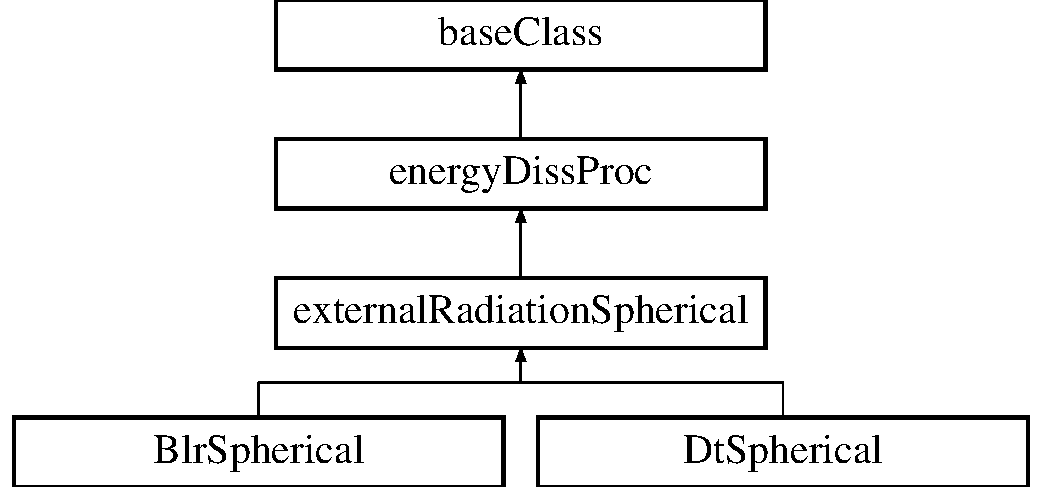
\includegraphics[height=4.000000cm]{classexternalRadiationSpherical}
\end{center}
\end{figure}


\subsection{Detailed Description}
Class provides electron energy losses and luminosity calculation for inverse Compton process (E\-R\-C) for seed photons comming from B\-L\-R and H\-D\-R modelled as spherical sources. Implementation provided by the class is identical to this in original B\-L\-A\-Z\-A\-R code from Moderski et al. (2003). it is not modified O\-R checked for consistency. Use with caution!

Class provides electron energy losses and luminosity calculation for inverse Compton process (E\-R\-C) for seed photons comming from B\-L\-R and H\-D\-R modelled as spherical sources \subsection*{Public Member Functions}
\begin{DoxyCompactItemize}
\item 
\hyperlink{classexternalRadiationSpherical_a8bc8c23cc374776d0c4431751dda67ed}{external\-Radiation\-Spherical} (scfgp $\ast$\-\_\-cfg, \hyperlink{classjetGeometry}{jet\-Geometry} $\ast$\-\_\-r, \hyperlink{classelectrons}{electrons} $\ast$\-\_\-ele, std\-::string \-\_\-id)
\item 
\hyperlink{classexternalRadiationSpherical_a9dbb13ad97d392d224e102a6f3eab62d}{$\sim$external\-Radiation\-Spherical} ()
\item 
virtual x void \hyperlink{classexternalRadiationSpherical_a560bd33ee97e6bdc7dc0d6138705e9b3}{set\-Radius} ()
\item 
virtual void \hyperlink{classexternalRadiationSpherical_a232684df0d246d8c5ec06e832bbaad0f}{print\-Info} ()
\item 
virtual void \hyperlink{classexternalRadiationSpherical_a05f5cf91c3a3c7844b167ff4476e64f8}{update} ()
\item 
virtual double \hyperlink{classexternalRadiationSpherical_a444023a18bd55023dc806bd0acccb7a0}{getvext} (double \-\_\-r)
\item 
double \hyperlink{classexternalRadiationSpherical_a96a2857022de4cc79852824610943910}{dotg} (double g)
\item 
double \hyperlink{classexternalRadiationSpherical_ac30f8dcecd62a05ff85140112c4e9b9c}{calculate\-Lpv} (double v, double theta)
\item 
void \hyperlink{classexternalRadiationSpherical_a2868df3597900f03c135baef15c825a8}{set\-Lpv} ()
\end{DoxyCompactItemize}
\subsection*{Public Attributes}
\begin{DoxyCompactItemize}
\item 
\hypertarget{classexternalRadiationSpherical_aed35674ef479631d23c334fe877b249b}{double {\bfseries cf}}\label{classexternalRadiationSpherical_aed35674ef479631d23c334fe877b249b}

\item 
\hypertarget{classexternalRadiationSpherical_aa345975e8ba7513f78e8bceedc276ef2}{double {\bfseries e}}\label{classexternalRadiationSpherical_aa345975e8ba7513f78e8bceedc276ef2}

\item 
\hypertarget{classexternalRadiationSpherical_a2ab4e8e8d8c11d30dfb6995f5dd12fbf}{double {\bfseries Gamma}}\label{classexternalRadiationSpherical_a2ab4e8e8d8c11d30dfb6995f5dd12fbf}

\item 
\hypertarget{classexternalRadiationSpherical_a55b1d81d349c305d1e0ad8f1f20b1c62}{double {\bfseries theta\-Obs}}\label{classexternalRadiationSpherical_a55b1d81d349c305d1e0ad8f1f20b1c62}

\item 
\hypertarget{classexternalRadiationSpherical_ae1e077ff5e8eaf52933b242ff6ff4e46}{int {\bfseries K\-N}}\label{classexternalRadiationSpherical_ae1e077ff5e8eaf52933b242ff6ff4e46}

\item 
\hypertarget{classexternalRadiationSpherical_a77b0da335c6c8442e1e95c0bb3cd5b36}{gsl\-\_\-vector $\ast$ {\bfseries upe}}\label{classexternalRadiationSpherical_a77b0da335c6c8442e1e95c0bb3cd5b36}

\end{DoxyCompactItemize}


\subsection{Constructor \& Destructor Documentation}
\hypertarget{classexternalRadiationSpherical_a8bc8c23cc374776d0c4431751dda67ed}{\index{external\-Radiation\-Spherical@{external\-Radiation\-Spherical}!external\-Radiation\-Spherical@{external\-Radiation\-Spherical}}
\index{external\-Radiation\-Spherical@{external\-Radiation\-Spherical}!externalRadiationSpherical@{external\-Radiation\-Spherical}}
\subsubsection[{external\-Radiation\-Spherical}]{\setlength{\rightskip}{0pt plus 5cm}external\-Radiation\-Spherical\-::external\-Radiation\-Spherical (
\begin{DoxyParamCaption}
\item[{scfgp $\ast$}]{\-\_\-cfg, }
\item[{{\bf jet\-Geometry} $\ast$}]{\-\_\-r, }
\item[{{\bf electrons} $\ast$}]{\-\_\-ele, }
\item[{std\-::string}]{\-\_\-id}
\end{DoxyParamCaption}
)}}\label{classexternalRadiationSpherical_a8bc8c23cc374776d0c4431751dda67ed}
constructor 
\begin{DoxyParams}{Parameters}
{\em \-\_\-cfg} & -\/ scfgp class object \\
\hline
{\em \-\_\-r} & -\/ \hyperlink{classjetGeometry}{jet\-Geometry} class object \\
\hline
{\em \-\_\-ele} & -\/ electrons class object \\
\hline
{\em \-\_\-id} & \\
\hline
\end{DoxyParams}

\begin{DoxyCode}
9                                                                                                            
                : \hyperlink{classenergyDissProc_a0cf0b423089016fbe8a697378c519590}{energyDissProc}( \_cfg, \_r, \_ele, \_id ) \{
10   \textcolor{comment}{/* requested parameters */}
11   \hyperlink{classbaseClass_a744f87a6ebe63da08256c022d42a4ca7}{cfg} -> request<int>(\textcolor{stringliteral}{"N"} + \hyperlink{classbaseClass_a4d5ff386a69bcbe21b5976f55b624df6}{id}, 200, &\hyperlink{classbaseClass_a2b4d07d2b46197d495de0477f4bb22f8}{N} );
12   \hyperlink{classbaseClass_a744f87a6ebe63da08256c022d42a4ca7}{cfg} -> request<double>(\textcolor{keywordtype}{id} + \textcolor{stringliteral}{"e"}, 1.0, &e );
13   \hyperlink{classbaseClass_a744f87a6ebe63da08256c022d42a4ca7}{cfg} -> request<double>(\textcolor{keywordtype}{id} + \textcolor{stringliteral}{"cf"}, 0.1, &cf );
14   \hyperlink{classbaseClass_a744f87a6ebe63da08256c022d42a4ca7}{cfg} -> request<double>(\textcolor{stringliteral}{"Gamma"}, 10.0, &Gamma );
15   \hyperlink{classbaseClass_a744f87a6ebe63da08256c022d42a4ca7}{cfg} -> request<double>(\textcolor{stringliteral}{"thetaObs"}, 0.1, &thetaObs );
16   \hyperlink{classbaseClass_a744f87a6ebe63da08256c022d42a4ca7}{cfg} -> request<int>(\textcolor{stringliteral}{"KN"}, 0, &KN );
17   \hyperlink{classbaseClass_a744f87a6ebe63da08256c022d42a4ca7}{cfg} -> request<int>(\textcolor{keywordtype}{id}+\textcolor{stringliteral}{"LuminosityConstU"},0,&\hyperlink{classenergyDissProc_a2cc4e4eae15982f977a0dfa5458d80f4}{luminosityConstU});  
18   \hyperlink{classbaseClass_a744f87a6ebe63da08256c022d42a4ca7}{cfg} -> request<int>(\textcolor{keywordtype}{id}+\textcolor{stringliteral}{"LuminosityConstNu"},0,&\hyperlink{classenergyDissProc_a0a23854c1c830dfb9ac33d116fce5b7d}{luminosityConstNu});  
19 
20   \hyperlink{classbaseClass_a744f87a6ebe63da08256c022d42a4ca7}{cfg} -> updateRequests( );
21 
22   \textcolor{comment}{/* allocate space for upe vector */}
23   upe = gsl\_vector\_alloc( \hyperlink{classbaseClass_a482bb9b1d94f3eb3f31026d14e9a2bb6}{r}->getMaxIndex( ) );
24   gsl\_vector\_set\_zero( upe );
25 
26   allocateUpeR( ); \}
\end{DoxyCode}
\hypertarget{classexternalRadiationSpherical_a9dbb13ad97d392d224e102a6f3eab62d}{\index{external\-Radiation\-Spherical@{external\-Radiation\-Spherical}!$\sim$external\-Radiation\-Spherical@{$\sim$external\-Radiation\-Spherical}}
\index{$\sim$external\-Radiation\-Spherical@{$\sim$external\-Radiation\-Spherical}!externalRadiationSpherical@{external\-Radiation\-Spherical}}
\subsubsection[{$\sim$external\-Radiation\-Spherical}]{\setlength{\rightskip}{0pt plus 5cm}external\-Radiation\-Spherical\-::$\sim$external\-Radiation\-Spherical (
\begin{DoxyParamCaption}
{}
\end{DoxyParamCaption}
)}}\label{classexternalRadiationSpherical_a9dbb13ad97d392d224e102a6f3eab62d}
destructor 
\begin{DoxyCode}
28                                                          \{
29   freeUpe( );
30   freeLpv( );
31   freeLvPoint( );
32   freeLvPointAvg( );
33   freeUpeR( );
34 
35   \textcolor{comment}{/* free space for upe vector */}
36   gsl\_vector\_free( upe );
37   upe = NULL; \}
\end{DoxyCode}


\subsection{Member Function Documentation}
\hypertarget{classexternalRadiationSpherical_ac30f8dcecd62a05ff85140112c4e9b9c}{\index{external\-Radiation\-Spherical@{external\-Radiation\-Spherical}!calculate\-Lpv@{calculate\-Lpv}}
\index{calculate\-Lpv@{calculate\-Lpv}!externalRadiationSpherical@{external\-Radiation\-Spherical}}
\subsubsection[{calculate\-Lpv}]{\setlength{\rightskip}{0pt plus 5cm}double external\-Radiation\-Spherical\-::calculate\-Lpv (
\begin{DoxyParamCaption}
\item[{double}]{v, }
\item[{double}]{theta}
\end{DoxyParamCaption}
)}}\label{classexternalRadiationSpherical_ac30f8dcecd62a05ff85140112c4e9b9c}
calculate intrinsic luminosity 
\begin{DoxyParams}{Parameters}
{\em v} & -\/ frequency (jet co-\/moving frame) \\
\hline
\end{DoxyParams}
\begin{DoxyReturn}{Returns}
L'\-\_\-v 
\end{DoxyReturn}

\begin{DoxyCode}
46                                                                         \{
47   \textcolor{keywordtype}{double} Int = 0.0;
48   \textcolor{keywordtype}{double} e, miu, \hyperlink{classenergyDissProc_a36330825cd7737639d5d223281b1c7e1}{ep};
49 
50   e = PLANCK\_H*v/mec2;
51   miu = -( cos(theta)-\hyperlink{classbaseClass_a208facecf3a4480b47bebfce91413a39}{beta}(Gamma) )/( 1.0-\hyperlink{classbaseClass_a208facecf3a4480b47bebfce91413a39}{beta}(Gamma)*cos(theta) );
52   ep = \hyperlink{classexternalRadiationSpherical_a444023a18bd55023dc806bd0acccb7a0}{getvext}( \hyperlink{classbaseClass_a482bb9b1d94f3eb3f31026d14e9a2bb6}{r}->get( ) )*PLANCK\_H*Gamma/mec2;
53 
54   \textcolor{keywordflow}{for}( \textcolor{keywordtype}{int} k=0;k<\hyperlink{classenergyDissProc_a0dbf0777938131e938c1fdad5df38a7f}{ele}->\hyperlink{classbaseClass_a6ba5c4ce24742db73f45064337cf6963}{getN}( );k++ )
55     Int  += bazinga::IntCor( k, \hyperlink{classenergyDissProc_a0dbf0777938131e938c1fdad5df38a7f}{ele}->\hyperlink{classbaseClass_a6ba5c4ce24742db73f45064337cf6963}{getN}( ) )*inverseCompton::f( \hyperlink{classenergyDissProc_a0dbf0777938131e938c1fdad5df38a7f}{ele}->
      \hyperlink{classelectrons_afb0d9365f13787f44d23fb489732fc90}{getGamma}(k), \hyperlink{classenergyDissProc_a36330825cd7737639d5d223281b1c7e1}{ep}, e, miu )*\hyperlink{classenergyDissProc_a0dbf0777938131e938c1fdad5df38a7f}{ele}->\hyperlink{classelectrons_a24fbbed0acac968ce6b2ef2c5043dee4}{getNgamma}(k)/\hyperlink{classenergyDissProc_a0dbf0777938131e938c1fdad5df38a7f}{ele}->
      \hyperlink{classelectrons_afb0d9365f13787f44d23fb489732fc90}{getGamma}(k);
56 
57   \textcolor{keywordflow}{if}( \hyperlink{classenergyDissProc_a2cc4e4eae15982f977a0dfa5458d80f4}{luminosityConstU} )
58     Int *= gsl\_vector\_get( upe, 0 )*\hyperlink{classenergyDissProc_a0dbf0777938131e938c1fdad5df38a7f}{ele}->\hyperlink{classelectrons_a4e3d4179ce211bd732580b49914874e6}{getdLogGamma}( )/pow( 
      \hyperlink{classexternalRadiationSpherical_a444023a18bd55023dc806bd0acccb7a0}{getvext}( \hyperlink{classbaseClass_a482bb9b1d94f3eb3f31026d14e9a2bb6}{r}->get( ) ), 2.0 );
59   \textcolor{keywordflow}{else} 
60     Int *= gsl\_vector\_get( upe, \hyperlink{classbaseClass_a482bb9b1d94f3eb3f31026d14e9a2bb6}{r}->getIndex( ) )*\hyperlink{classenergyDissProc_a0dbf0777938131e938c1fdad5df38a7f}{ele}->\hyperlink{classelectrons_a4e3d4179ce211bd732580b49914874e6}{getdLogGamma}( )/pow( 
      \hyperlink{classexternalRadiationSpherical_a444023a18bd55023dc806bd0acccb7a0}{getvext}( \hyperlink{classbaseClass_a482bb9b1d94f3eb3f31026d14e9a2bb6}{r}->get( ) ), 2.0 );
61 
62   Int *= (3.0*SIGMA\_T*LIGHT\_SPEED)/(4.0*pow(Gamma,2.0));
63   Int *= v;
64   \textcolor{keywordflow}{return} Int; \}
\end{DoxyCode}
\hypertarget{classexternalRadiationSpherical_a96a2857022de4cc79852824610943910}{\index{external\-Radiation\-Spherical@{external\-Radiation\-Spherical}!dotg@{dotg}}
\index{dotg@{dotg}!externalRadiationSpherical@{external\-Radiation\-Spherical}}
\subsubsection[{dotg}]{\setlength{\rightskip}{0pt plus 5cm}double external\-Radiation\-Spherical\-::dotg (
\begin{DoxyParamCaption}
\item[{double}]{g}
\end{DoxyParamCaption}
)\hspace{0.3cm}{\ttfamily [virtual]}}}\label{classexternalRadiationSpherical_a96a2857022de4cc79852824610943910}
get d gamma \textbackslash{} d t for particular process 
\begin{DoxyParams}{Parameters}
{\em g} & -\/ electron Lorentz factor \\
\hline
\end{DoxyParams}
\begin{DoxyReturn}{Returns}
d gamma \textbackslash{} d t 
\end{DoxyReturn}


Reimplemented from \hyperlink{classenergyDissProc_a8074e0db5d859a8815e7136c2fc41b46}{energy\-Diss\-Proc}.


\begin{DoxyCode}
39                                                   \{
40   \textcolor{keywordtype}{double} b, val = 0.0;
41   b = 4.0*g*\hyperlink{classexternalRadiationSpherical_a444023a18bd55023dc806bd0acccb7a0}{getvext}( \hyperlink{classbaseClass_a482bb9b1d94f3eb3f31026d14e9a2bb6}{r}->get( ) )*PLANCK\_H*Gamma/mec2;
42   \textcolor{keywordflow}{if}( b > 1.0 ) \{ \hyperlink{classenergyDissProc_a69ea4be814273e47e69e31e593c3a250}{set\_KN\_info}( g ); \}
43   val = gsl\_vector\_get( upe, \hyperlink{classbaseClass_a482bb9b1d94f3eb3f31026d14e9a2bb6}{r}->getIndex( ) )*inverseCompton::fKN(b,KN); 
44   \textcolor{keywordflow}{return} val; \}
\end{DoxyCode}
\hypertarget{classexternalRadiationSpherical_a444023a18bd55023dc806bd0acccb7a0}{\index{external\-Radiation\-Spherical@{external\-Radiation\-Spherical}!getvext@{getvext}}
\index{getvext@{getvext}!externalRadiationSpherical@{external\-Radiation\-Spherical}}
\subsubsection[{getvext}]{\setlength{\rightskip}{0pt plus 5cm}virtual double external\-Radiation\-Spherical\-::getvext (
\begin{DoxyParamCaption}
\item[{double}]{\-\_\-r}
\end{DoxyParamCaption}
)\hspace{0.3cm}{\ttfamily [inline]}, {\ttfamily [virtual]}}}\label{classexternalRadiationSpherical_a444023a18bd55023dc806bd0acccb7a0}
now obsolete virtual double getd\-Ldlnr( double \-\_\-r ) \{ return 0; \} get v\-\_\-ext value in Hz 
\begin{DoxyParams}{Parameters}
{\em \-\_\-r} & -\/ radius \\
\hline
\end{DoxyParams}
\begin{DoxyReturn}{Returns}
v\-\_\-ext 
\end{DoxyReturn}


Reimplemented in \hyperlink{classDtSpherical_a25a9bd3b5a47e2d1428325614686f5ac}{Dt\-Spherical}, and \hyperlink{classBlrSpherical_aaf00f59d04b5e193aa47959dd1cc1065}{Blr\-Spherical}.


\begin{DoxyCode}
52 \{ \textcolor{keywordflow}{return} 0; \}
\end{DoxyCode}
\hypertarget{classexternalRadiationSpherical_a232684df0d246d8c5ec06e832bbaad0f}{\index{external\-Radiation\-Spherical@{external\-Radiation\-Spherical}!print\-Info@{print\-Info}}
\index{print\-Info@{print\-Info}!externalRadiationSpherical@{external\-Radiation\-Spherical}}
\subsubsection[{print\-Info}]{\setlength{\rightskip}{0pt plus 5cm}virtual void external\-Radiation\-Spherical\-::print\-Info (
\begin{DoxyParamCaption}
{}
\end{DoxyParamCaption}
)\hspace{0.3cm}{\ttfamily [inline]}, {\ttfamily [virtual]}}}\label{classexternalRadiationSpherical_a232684df0d246d8c5ec06e832bbaad0f}
print basic information about myself (virtual) 

Reimplemented from \hyperlink{classenergyDissProc_ad1fbde0f7635a19a81412b9766916eb9}{energy\-Diss\-Proc}.



Reimplemented in \hyperlink{classDtSpherical_a14440ec30b997fe2461c07f4507dd994}{Dt\-Spherical}, and \hyperlink{classBlrSpherical_a101b95271855f15f1049fcea9efde235}{Blr\-Spherical}.


\begin{DoxyCode}
41 \{ \}
\end{DoxyCode}
\hypertarget{classexternalRadiationSpherical_a2868df3597900f03c135baef15c825a8}{\index{external\-Radiation\-Spherical@{external\-Radiation\-Spherical}!set\-Lpv@{set\-Lpv}}
\index{set\-Lpv@{set\-Lpv}!externalRadiationSpherical@{external\-Radiation\-Spherical}}
\subsubsection[{set\-Lpv}]{\setlength{\rightskip}{0pt plus 5cm}void external\-Radiation\-Spherical\-::set\-Lpv (
\begin{DoxyParamCaption}
{}
\end{DoxyParamCaption}
)\hspace{0.3cm}{\ttfamily [virtual]}}}\label{classexternalRadiationSpherical_a2868df3597900f03c135baef15c825a8}
set intrinsic luminosities 

Reimplemented from \hyperlink{classenergyDissProc_a93a39df53f30801f9f057cd55c05485d}{energy\-Diss\-Proc}.


\begin{DoxyCode}
66                                          \{
67   \textcolor{keywordflow}{for}( \textcolor{keywordtype}{int} i=0;i<\hyperlink{classbaseClass_a2b4d07d2b46197d495de0477f4bb22f8}{N};i++ ) \{ set\_Lpv( i, \hyperlink{classexternalRadiationSpherical_ac30f8dcecd62a05ff85140112c4e9b9c}{calculateLpv}( get\_vp(i),thetaObs ) ); \}
68 \}
\end{DoxyCode}
\hypertarget{classexternalRadiationSpherical_a560bd33ee97e6bdc7dc0d6138705e9b3}{\index{external\-Radiation\-Spherical@{external\-Radiation\-Spherical}!set\-Radius@{set\-Radius}}
\index{set\-Radius@{set\-Radius}!externalRadiationSpherical@{external\-Radiation\-Spherical}}
\subsubsection[{set\-Radius}]{\setlength{\rightskip}{0pt plus 5cm}virtual x void external\-Radiation\-Spherical\-::set\-Radius (
\begin{DoxyParamCaption}
{}
\end{DoxyParamCaption}
)\hspace{0.3cm}{\ttfamily [inline]}, {\ttfamily [virtual]}}}\label{classexternalRadiationSpherical_a560bd33ee97e6bdc7dc0d6138705e9b3}
sets rext if not provided by config file 

Reimplemented in \hyperlink{classDtSpherical_aac1ed31d84f539e4e372bc1a567e4555}{Dt\-Spherical}, and \hyperlink{classBlrSpherical_adc2876b14e36b86f5a35d31c708d5d35}{Blr\-Spherical}.


\begin{DoxyCode}
40 \{ \}
\end{DoxyCode}
\hypertarget{classexternalRadiationSpherical_a05f5cf91c3a3c7844b167ff4476e64f8}{\index{external\-Radiation\-Spherical@{external\-Radiation\-Spherical}!update@{update}}
\index{update@{update}!externalRadiationSpherical@{external\-Radiation\-Spherical}}
\subsubsection[{update}]{\setlength{\rightskip}{0pt plus 5cm}virtual void external\-Radiation\-Spherical\-::update (
\begin{DoxyParamCaption}
{}
\end{DoxyParamCaption}
)\hspace{0.3cm}{\ttfamily [inline]}, {\ttfamily [virtual]}}}\label{classexternalRadiationSpherical_a05f5cf91c3a3c7844b167ff4476e64f8}
calculate and set Upe every time with new radius r 

Reimplemented from \hyperlink{classenergyDissProc_a6033524ea3d0fe38056bd74622f6c4ad}{energy\-Diss\-Proc}.



Reimplemented in \hyperlink{classDtSpherical_ab9844cfdd3df5bc213bf93dd7b320bb7}{Dt\-Spherical}, and \hyperlink{classBlrSpherical_ad67ab24f0b7f0ec3a0893fd2e3170f6c}{Blr\-Spherical}.


\begin{DoxyCode}
44 \{ \}
\end{DoxyCode}


The documentation for this class was generated from the following files\-:\begin{DoxyCompactItemize}
\item 
/home/mjaniak/\-Soft/blazar++/include/\hyperlink{externalRadiationSpherical_8hpp}{external\-Radiation\-Spherical.\-hpp}\item 
/home/mjaniak/\-Soft/blazar++/src/\hyperlink{externalRadiationSpherical_8cpp}{external\-Radiation\-Spherical.\-cpp}\end{DoxyCompactItemize}

\hypertarget{structgamma__break__params}{\section{gamma\-\_\-break\-\_\-params Struct Reference}
\label{structgamma__break__params}\index{gamma\-\_\-break\-\_\-params@{gamma\-\_\-break\-\_\-params}}
}
\subsection*{Public Attributes}
\begin{DoxyCompactItemize}
\item 
\hypertarget{structgamma__break__params_ab15a7252bff47351128cde2d58ed9bf3}{double {\bfseries p1}}\label{structgamma__break__params_ab15a7252bff47351128cde2d58ed9bf3}

\item 
\hypertarget{structgamma__break__params_a4b8ccd0d1a10e20083e659cde93a9c2b}{double {\bfseries p2}}\label{structgamma__break__params_a4b8ccd0d1a10e20083e659cde93a9c2b}

\item 
\hypertarget{structgamma__break__params_a3bc9e32ac0e8640107711c06ffd8610c}{double {\bfseries gamma\-\_\-min}}\label{structgamma__break__params_a3bc9e32ac0e8640107711c06ffd8610c}

\item 
\hypertarget{structgamma__break__params_ac22a6a8ec4c755a6418a811d1d90dffb}{double {\bfseries gamma\-\_\-max}}\label{structgamma__break__params_ac22a6a8ec4c755a6418a811d1d90dffb}

\item 
\hypertarget{structgamma__break__params_a1c2c2c67b6a3ae2a370359ca37fd57fc}{double {\bfseries avg\-\_\-gamma}}\label{structgamma__break__params_a1c2c2c67b6a3ae2a370359ca37fd57fc}

\end{DoxyCompactItemize}


The documentation for this struct was generated from the following file\-:\begin{DoxyCompactItemize}
\item 
/home/mjaniak/\-Soft/blazar++/include/\hyperlink{electrons_8hpp}{electrons.\-hpp}\end{DoxyCompactItemize}

\hypertarget{classjetGeometry}{\section{jet\-Geometry Class Reference}
\label{classjetGeometry}\index{jet\-Geometry@{jet\-Geometry}}
}
\subsection*{Public Member Functions}
\begin{DoxyCompactItemize}
\item 
\hypertarget{classjetGeometry_a4ca3e81d2ce21b08e8df9638eb094b33}{{\bfseries jet\-Geometry} (scfgp $\ast$\-\_\-cfg)}\label{classjetGeometry_a4ca3e81d2ce21b08e8df9638eb094b33}

\item 
\hypertarget{classjetGeometry_a8fb63607bae0a7ec9829d1cbf62cba76}{void {\bfseries update} (int index)}\label{classjetGeometry_a8fb63607bae0a7ec9829d1cbf62cba76}

\item 
\hypertarget{classjetGeometry_a8594bcbc6a54649cedea0cb2ec77c1d8}{double {\bfseries show} ()}\label{classjetGeometry_a8594bcbc6a54649cedea0cb2ec77c1d8}

\item 
\hypertarget{classjetGeometry_a0596785494429f321d8c222896069b66}{double {\bfseries get} ()}\label{classjetGeometry_a0596785494429f321d8c222896069b66}

\item 
\hypertarget{classjetGeometry_a65ae1b4112255e05c15fdddd79328d1d}{double {\bfseries get} (int index)}\label{classjetGeometry_a65ae1b4112255e05c15fdddd79328d1d}

\item 
\hypertarget{classjetGeometry_adf1862920d3b2d378ae3a69adb6925df}{int {\bfseries get\-Index} ()}\label{classjetGeometry_adf1862920d3b2d378ae3a69adb6925df}

\item 
\hypertarget{classjetGeometry_ac164863c15809691e3160b11253c4a11}{int {\bfseries get\-Max\-Index} ()}\label{classjetGeometry_ac164863c15809691e3160b11253c4a11}

\item 
\hypertarget{classjetGeometry_abb4bfa533ecdb5fc651daab48902205a}{double {\bfseries get\-Dr} ()}\label{classjetGeometry_abb4bfa533ecdb5fc651daab48902205a}

\item 
\hypertarget{classjetGeometry_a1bb18dbf002061c08d7695a93edd3530}{double {\bfseries get\-Dr} (int index)}\label{classjetGeometry_a1bb18dbf002061c08d7695a93edd3530}

\item 
\hypertarget{classjetGeometry_ad5b17b9b6be29fda8b8c012347142c17}{double {\bfseries get\-Position} ()}\label{classjetGeometry_ad5b17b9b6be29fda8b8c012347142c17}

\item 
\hypertarget{classjetGeometry_a3490dafbe35896560ba2cc9ef1461f10}{double {\bfseries get\-Position} (int index)}\label{classjetGeometry_a3490dafbe35896560ba2cc9ef1461f10}

\item 
\hypertarget{classjetGeometry_a4a2386eda15f16e6c0a24433116898d8}{void {\bfseries print\-Info} ()}\label{classjetGeometry_a4a2386eda15f16e6c0a24433116898d8}

\item 
\hypertarget{classjetGeometry_ae66c12983e87c67a1c7601a53389575f}{int {\bfseries get\-Ninj} ()}\label{classjetGeometry_ae66c12983e87c67a1c7601a53389575f}

\item 
\hypertarget{classjetGeometry_ad0ab1140dc51cfa933b94254d659fe23}{double {\bfseries get\-R0} ()}\label{classjetGeometry_ad0ab1140dc51cfa933b94254d659fe23}

\item 
\hypertarget{classjetGeometry_ad97dbfdf7252e15d297d4c0696eff76b}{double {\bfseries get\-R\-Inj\-Max} ()}\label{classjetGeometry_ad97dbfdf7252e15d297d4c0696eff76b}

\item 
\hypertarget{classjetGeometry_ab2104e4f24e6733e8179d07b4faca1b1}{double {\bfseries get\-R\-Max} ()}\label{classjetGeometry_ab2104e4f24e6733e8179d07b4faca1b1}

\item 
\hypertarget{classjetGeometry_a54eed30a1333c075545f0aae18d9f8f7}{gsl\-\_\-vector $\ast$ {\bfseries get\-Radius\-\_\-\-G\-S\-L\-Vector} ()}\label{classjetGeometry_a54eed30a1333c075545f0aae18d9f8f7}

\item 
\hypertarget{classjetGeometry_a5422d39d309d07f4f3eee857397b8247}{int {\bfseries if\-Save\-Radius} ()}\label{classjetGeometry_a5422d39d309d07f4f3eee857397b8247}

\end{DoxyCompactItemize}


The documentation for this class was generated from the following files\-:\begin{DoxyCompactItemize}
\item 
/home/mjaniak/\-Soft/blazar++/include/jet\-Geometry.\-hpp\item 
/home/mjaniak/\-Soft/blazar++/src/jet\-Geometry.\-cpp\end{DoxyCompactItemize}

\hypertarget{classlogGeometry}{\section{log\-Geometry Class Reference}
\label{classlogGeometry}\index{log\-Geometry@{log\-Geometry}}
}
\subsection*{Public Member Functions}
\begin{DoxyCompactItemize}
\item 
\hypertarget{classlogGeometry_acbe7e42d84d706ca2e393931354e4f80}{{\bfseries log\-Geometry} (double \-\_\-r1, double \-\_\-r2, double \-\_\-\-N)}\label{classlogGeometry_acbe7e42d84d706ca2e393931354e4f80}

\item 
\hypertarget{classlogGeometry_a6bd19dfc09f969fec401802fd0a33c20}{void {\bfseries update} (int index)}\label{classlogGeometry_a6bd19dfc09f969fec401802fd0a33c20}

\item 
\hypertarget{classlogGeometry_afb47230469268443d3ba07a516522e1d}{double {\bfseries show} ()}\label{classlogGeometry_afb47230469268443d3ba07a516522e1d}

\item 
\hypertarget{classlogGeometry_aa76e4cd005253fb843e560fe84f07b97}{double {\bfseries get} ()}\label{classlogGeometry_aa76e4cd005253fb843e560fe84f07b97}

\item 
\hypertarget{classlogGeometry_a344599f7790e01d64dea6da88d5d78bb}{double {\bfseries get} (int index)}\label{classlogGeometry_a344599f7790e01d64dea6da88d5d78bb}

\item 
\hypertarget{classlogGeometry_af214c858d7d96eb6e4233cb310112f08}{int {\bfseries get\-Index} ()}\label{classlogGeometry_af214c858d7d96eb6e4233cb310112f08}

\item 
\hypertarget{classlogGeometry_a98c824014ee3b73d81251b9c17667ebb}{int {\bfseries get\-Max\-Index} ()}\label{classlogGeometry_a98c824014ee3b73d81251b9c17667ebb}

\item 
\hypertarget{classlogGeometry_a5db13e9f817b91ce4e618a28c716b93c}{double {\bfseries get\-Dr} ()}\label{classlogGeometry_a5db13e9f817b91ce4e618a28c716b93c}

\item 
\hypertarget{classlogGeometry_a42413b8e326afeef7cd6fa57ca99732c}{double {\bfseries get\-Dr} (int index)}\label{classlogGeometry_a42413b8e326afeef7cd6fa57ca99732c}

\item 
\hypertarget{classlogGeometry_aaca3ce8b82281a8000d8d8cfb4762998}{double {\bfseries get\-Position} ()}\label{classlogGeometry_aaca3ce8b82281a8000d8d8cfb4762998}

\item 
\hypertarget{classlogGeometry_a8339ccfa0b3051709fd0386c06253ad9}{double {\bfseries get\-Position} (int index)}\label{classlogGeometry_a8339ccfa0b3051709fd0386c06253ad9}

\item 
\hypertarget{classlogGeometry_af4167416bf80d5e0c6cd520c1d4530e7}{void {\bfseries print\-Info} ()}\label{classlogGeometry_af4167416bf80d5e0c6cd520c1d4530e7}

\item 
\hypertarget{classlogGeometry_a80244c6af7c29c4980c67a8b1118e518}{double {\bfseries get\-R0} ()}\label{classlogGeometry_a80244c6af7c29c4980c67a8b1118e518}

\item 
\hypertarget{classlogGeometry_a44f4c2f05b49d5611af4469209388cc1}{double {\bfseries get\-R\-Max} ()}\label{classlogGeometry_a44f4c2f05b49d5611af4469209388cc1}

\item 
\hypertarget{classlogGeometry_ad147a417537a8725770955eba55d0ec0}{int {\bfseries get\-N} ()}\label{classlogGeometry_ad147a417537a8725770955eba55d0ec0}

\item 
\hypertarget{classlogGeometry_aa6f086bdef4ffe3094e46ea26a011672}{gsl\-\_\-vector $\ast$ {\bfseries get\-Radius\-\_\-\-G\-S\-L\-Vector} ()}\label{classlogGeometry_aa6f086bdef4ffe3094e46ea26a011672}

\end{DoxyCompactItemize}


The documentation for this class was generated from the following files\-:\begin{DoxyCompactItemize}
\item 
/home/mjaniak/\-Soft/blazar++/include/log\-Geometry.\-hpp\item 
/home/mjaniak/\-Soft/blazar++/src/log\-Geometry.\-cpp\end{DoxyCompactItemize}

\hypertarget{classmagneticField}{\section{magnetic\-Field Class Reference}
\label{classmagneticField}\index{magnetic\-Field@{magnetic\-Field}}
}


{\ttfamily \#include $<$magnetic\-Field.\-hpp$>$}

Inheritance diagram for magnetic\-Field\-:\begin{figure}[H]
\begin{center}
\leavevmode
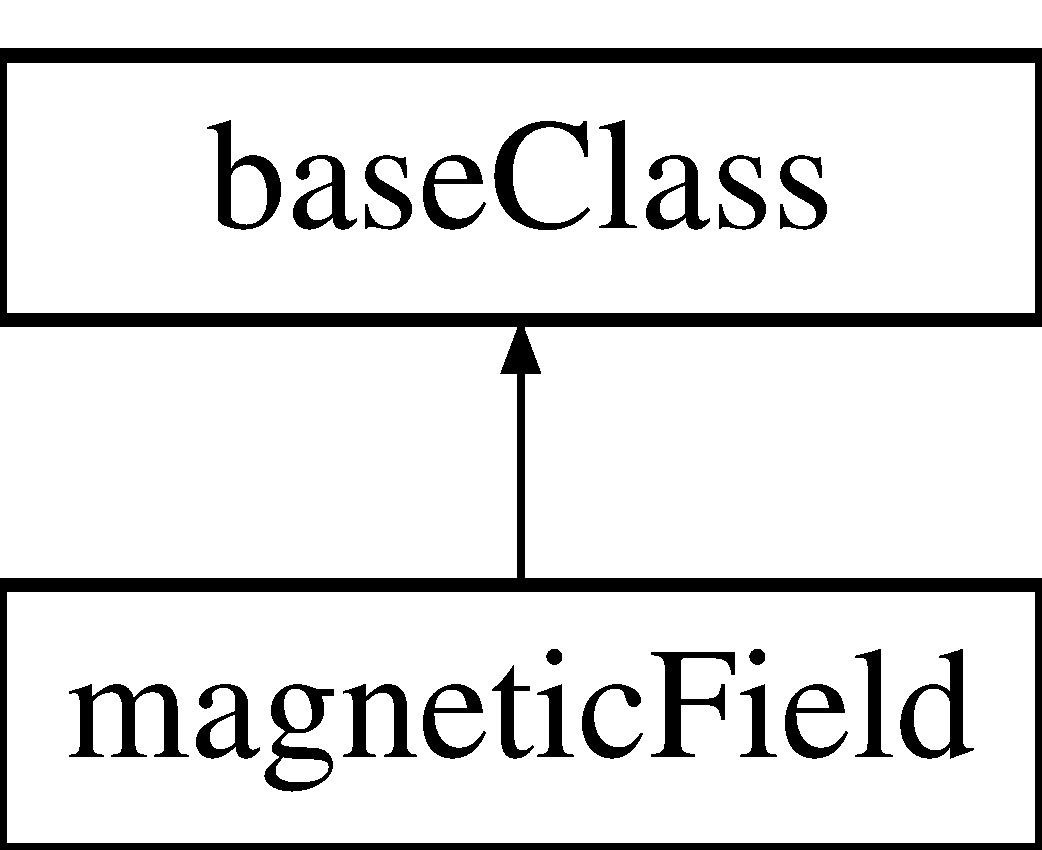
\includegraphics[height=2.000000cm]{classmagneticField}
\end{center}
\end{figure}


\subsection{Detailed Description}
Class defining magnetic field across the jet \subsection*{Public Member Functions}
\begin{DoxyCompactItemize}
\item 
\hyperlink{classmagneticField_ac856f6e43cc63fb2a16c0f013d70123b}{magnetic\-Field} (scfgp $\ast$\-\_\-cfg, \hyperlink{classjetGeometry}{jet\-Geometry} $\ast$\-\_\-r, std\-::string \-\_\-id)
\item 
\hyperlink{classmagneticField_a1d7c41029c88b3a2683d8e1bec376e16}{$\sim$magnetic\-Field} ()
\item 
double \hyperlink{classmagneticField_ac345cd6d5a111f0b96db08dadf65ff76}{get\-B} ()
\item 
double \hyperlink{classmagneticField_a24bacbdab7f8c280e0bcbbe8ff50e5eb}{get\-B} (double \-\_\-r)
\item 
double \hyperlink{classmagneticField_a3b573d12649137290d521539b903da8d}{get\-Max\-B} ()
\item 
double \hyperlink{classmagneticField_ad1184833ba01cf9ef3fdf4bbd5b6f7f9}{get\-\_\-u\-B} ()
\item 
double \hyperlink{classmagneticField_ad9d8d66260564c919d0fd253f4b3c60d}{get\-\_\-u\-B} (double \-\_\-r)
\item 
void \hyperlink{classmagneticField_a9a0793b3b3a94962aaea1052edfe9b28}{print\-Info} ()
\end{DoxyCompactItemize}
\subsection*{Additional Inherited Members}


\subsection{Constructor \& Destructor Documentation}
\hypertarget{classmagneticField_ac856f6e43cc63fb2a16c0f013d70123b}{\index{magnetic\-Field@{magnetic\-Field}!magnetic\-Field@{magnetic\-Field}}
\index{magnetic\-Field@{magnetic\-Field}!magneticField@{magnetic\-Field}}
\subsubsection[{magnetic\-Field}]{\setlength{\rightskip}{0pt plus 5cm}magnetic\-Field\-::magnetic\-Field (
\begin{DoxyParamCaption}
\item[{scfgp $\ast$}]{\-\_\-cfg, }
\item[{{\bf jet\-Geometry} $\ast$}]{\-\_\-r, }
\item[{std\-::string}]{\-\_\-id}
\end{DoxyParamCaption}
)}}\label{classmagneticField_ac856f6e43cc63fb2a16c0f013d70123b}
consructor 
\begin{DoxyParams}{Parameters}
{\em scfgp} & \\
\hline
{\em \hyperlink{classjetGeometry}{jet\-Geometry}} & \\
\hline
{\em id} & \\
\hline
\end{DoxyParams}

\begin{DoxyCode}
8                                                                           : 
      \hyperlink{classbaseClass}{baseClass}(\_cfg, \_r, \_id ) \{ 
9 
10   \textcolor{comment}{/* request parameters */}
11   \hyperlink{classbaseClass_a744f87a6ebe63da08256c022d42a4ca7}{cfg} -> request<double>(\textcolor{stringliteral}{"B0"},0.0,&B0);
12   \hyperlink{classbaseClass_a744f87a6ebe63da08256c022d42a4ca7}{cfg} -> request<double>(\textcolor{stringliteral}{"B1"},1.0,&B1);
13   \hyperlink{classbaseClass_a744f87a6ebe63da08256c022d42a4ca7}{cfg} -> request<double>(\textcolor{stringliteral}{"sigmaB"},0.01,&sigmaB);
14   \hyperlink{classbaseClass_a744f87a6ebe63da08256c022d42a4ca7}{cfg} -> request<double>(\textcolor{stringliteral}{"kB"},2.0,&kB);
15   \hyperlink{classbaseClass_a744f87a6ebe63da08256c022d42a4ca7}{cfg} -> request<std::string>(\textcolor{stringliteral}{"magModel"},\textcolor{stringliteral}{"blob"},&magModel);
16   \hyperlink{classbaseClass_a744f87a6ebe63da08256c022d42a4ca7}{cfg} -> request<double>(\textcolor{stringliteral}{"Gamma"},10.0,&Gamma);
17   \hyperlink{classbaseClass_a744f87a6ebe63da08256c022d42a4ca7}{cfg} -> request<double>(\textcolor{stringliteral}{"thetaJ"},0.1,&thetaJ);
18   \hyperlink{classbaseClass_a744f87a6ebe63da08256c022d42a4ca7}{cfg} -> request<double>(\textcolor{stringliteral}{"injRm"},2.0e17,&injRm);
19   \hyperlink{classbaseClass_a744f87a6ebe63da08256c022d42a4ca7}{cfg} -> request<double>(\textcolor{stringliteral}{"eDiss"},0.1,&eDiss);
20   \hyperlink{classbaseClass_a744f87a6ebe63da08256c022d42a4ca7}{cfg} -> request<double>(\textcolor{stringliteral}{"eEle"},0.1,&eEle);
21   \hyperlink{classbaseClass_a744f87a6ebe63da08256c022d42a4ca7}{cfg} -> request<double>(\textcolor{stringliteral}{"mBH"},1.0,&mBH);
22   \hyperlink{classbaseClass_a744f87a6ebe63da08256c022d42a4ca7}{cfg} -> request<double>(\textcolor{stringliteral}{"eJet"},0.3,&eJet);
23   \hyperlink{classbaseClass_a744f87a6ebe63da08256c022d42a4ca7}{cfg} -> request<double>(\textcolor{stringliteral}{"mDot"},1.0,&mDot);
24 
25   \hyperlink{classbaseClass_a744f87a6ebe63da08256c022d42a4ca7}{cfg} -> updateRequests( );
26 
27   \textcolor{comment}{/* set energetics and magnetic flux value if in 'steady' model */}
28   \textcolor{keywordflow}{if}( magModel == \textcolor{stringliteral}{"steady"} ) \{
29     \textcolor{keywordtype}{double} Ledd, Ljet;
30     Ledd = 1.3e47*mBH;
31     Ljet = 0.5*eJet*mDot*Ledd;
32     Lb = sigmaB*(1.0-eDiss)*Ljet/(1.0+sigmaB);
33     B0steady = sqrt(6.0*Lb/(LIGHT\_SPEED*\hyperlink{classbaseClass_a208facecf3a4480b47bebfce91413a39}{beta}(Gamma)))/(thetaJ*Gamma); \}
34 \}
\end{DoxyCode}
\hypertarget{classmagneticField_a1d7c41029c88b3a2683d8e1bec376e16}{\index{magnetic\-Field@{magnetic\-Field}!$\sim$magnetic\-Field@{$\sim$magnetic\-Field}}
\index{$\sim$magnetic\-Field@{$\sim$magnetic\-Field}!magneticField@{magnetic\-Field}}
\subsubsection[{$\sim$magnetic\-Field}]{\setlength{\rightskip}{0pt plus 5cm}magnetic\-Field\-::$\sim$magnetic\-Field (
\begin{DoxyParamCaption}
{}
\end{DoxyParamCaption}
)}}\label{classmagneticField_a1d7c41029c88b3a2683d8e1bec376e16}
destructor 

\subsection{Member Function Documentation}
\hypertarget{classmagneticField_ad1184833ba01cf9ef3fdf4bbd5b6f7f9}{\index{magnetic\-Field@{magnetic\-Field}!get\-\_\-u\-B@{get\-\_\-u\-B}}
\index{get\-\_\-u\-B@{get\-\_\-u\-B}!magneticField@{magnetic\-Field}}
\subsubsection[{get\-\_\-u\-B}]{\setlength{\rightskip}{0pt plus 5cm}double magnetic\-Field\-::get\-\_\-u\-B (
\begin{DoxyParamCaption}
{}
\end{DoxyParamCaption}
)}}\label{classmagneticField_ad1184833ba01cf9ef3fdf4bbd5b6f7f9}
get current value of magnetic energy density 
\begin{DoxyCode}
65 \{ \textcolor{keywordflow}{return}( DSQR( \hyperlink{classmagneticField_ac345cd6d5a111f0b96db08dadf65ff76}{getB}( ) )/(8.0*M\_PI) ); \}
\end{DoxyCode}
\hypertarget{classmagneticField_ad9d8d66260564c919d0fd253f4b3c60d}{\index{magnetic\-Field@{magnetic\-Field}!get\-\_\-u\-B@{get\-\_\-u\-B}}
\index{get\-\_\-u\-B@{get\-\_\-u\-B}!magneticField@{magnetic\-Field}}
\subsubsection[{get\-\_\-u\-B}]{\setlength{\rightskip}{0pt plus 5cm}double magnetic\-Field\-::get\-\_\-u\-B (
\begin{DoxyParamCaption}
\item[{double}]{\-\_\-r}
\end{DoxyParamCaption}
)}}\label{classmagneticField_ad9d8d66260564c919d0fd253f4b3c60d}
get value of magnetic energy density at aspecific radius 
\begin{DoxyParams}{Parameters}
{\em radius} & \\
\hline
\end{DoxyParams}

\begin{DoxyCode}
66 \{ \textcolor{keywordflow}{return}( DSQR( \hyperlink{classmagneticField_ac345cd6d5a111f0b96db08dadf65ff76}{getB}( \_r ) )/(8.0*M\_PI) ); \}
\end{DoxyCode}
\hypertarget{classmagneticField_ac345cd6d5a111f0b96db08dadf65ff76}{\index{magnetic\-Field@{magnetic\-Field}!get\-B@{get\-B}}
\index{get\-B@{get\-B}!magneticField@{magnetic\-Field}}
\subsubsection[{get\-B}]{\setlength{\rightskip}{0pt plus 5cm}double magnetic\-Field\-::get\-B (
\begin{DoxyParamCaption}
{}
\end{DoxyParamCaption}
)}}\label{classmagneticField_ac345cd6d5a111f0b96db08dadf65ff76}
get current value of magnetic field 
\begin{DoxyCode}
50                             \{ 
51   \textcolor{keywordflow}{if}( magModel == \textcolor{stringliteral}{"steady"} ) \{ \textcolor{keywordflow}{return} B0steady/\hyperlink{classbaseClass_a482bb9b1d94f3eb3f31026d14e9a2bb6}{r}->get( ); \};
52   \textcolor{keywordflow}{if}( magModel == \textcolor{stringliteral}{"blob"} ) \{ \textcolor{keywordflow}{return} B0+(B1*pow(injRm/\hyperlink{classbaseClass_a482bb9b1d94f3eb3f31026d14e9a2bb6}{r}->get( ),0.5*kB)); \}
53 \}
\end{DoxyCode}
\hypertarget{classmagneticField_a24bacbdab7f8c280e0bcbbe8ff50e5eb}{\index{magnetic\-Field@{magnetic\-Field}!get\-B@{get\-B}}
\index{get\-B@{get\-B}!magneticField@{magnetic\-Field}}
\subsubsection[{get\-B}]{\setlength{\rightskip}{0pt plus 5cm}double magnetic\-Field\-::get\-B (
\begin{DoxyParamCaption}
\item[{double}]{\-\_\-r}
\end{DoxyParamCaption}
)}}\label{classmagneticField_a24bacbdab7f8c280e0bcbbe8ff50e5eb}
get value of magnetic field at specific radius 
\begin{DoxyParams}{Parameters}
{\em radius} & \\
\hline
\end{DoxyParams}

\begin{DoxyCode}
55                                       \{ 
56   \textcolor{keywordflow}{if}( magModel == \textcolor{stringliteral}{"steady"} ) \{ \textcolor{keywordflow}{return} B0steady/\_r; \};
57   \textcolor{keywordflow}{if}( magModel == \textcolor{stringliteral}{"blob"} ) \{ \textcolor{keywordflow}{return} B0+(B1*pow(injRm/\_r,0.5*kB)); \}
58 \}
\end{DoxyCode}
\hypertarget{classmagneticField_a3b573d12649137290d521539b903da8d}{\index{magnetic\-Field@{magnetic\-Field}!get\-Max\-B@{get\-Max\-B}}
\index{get\-Max\-B@{get\-Max\-B}!magneticField@{magnetic\-Field}}
\subsubsection[{get\-Max\-B}]{\setlength{\rightskip}{0pt plus 5cm}double magnetic\-Field\-::get\-Max\-B (
\begin{DoxyParamCaption}
{}
\end{DoxyParamCaption}
)}}\label{classmagneticField_a3b573d12649137290d521539b903da8d}
get maximum value of magnetic field (closest radius 
\begin{DoxyCode}
60                                \{
61   \textcolor{keywordflow}{if}( magModel == \textcolor{stringliteral}{"steady"} ) \{ \textcolor{keywordflow}{return} B0steady/\hyperlink{classbaseClass_a482bb9b1d94f3eb3f31026d14e9a2bb6}{r}->getR0( ); \}
62   \textcolor{keywordflow}{if}( magModel == \textcolor{stringliteral}{"blob"} ) \{ \textcolor{keywordflow}{return} B0+(B1*pow( injRm/\hyperlink{classbaseClass_a482bb9b1d94f3eb3f31026d14e9a2bb6}{r}->getR0( ),0.5*kB)); \}
63 \}
\end{DoxyCode}
\hypertarget{classmagneticField_a9a0793b3b3a94962aaea1052edfe9b28}{\index{magnetic\-Field@{magnetic\-Field}!print\-Info@{print\-Info}}
\index{print\-Info@{print\-Info}!magneticField@{magnetic\-Field}}
\subsubsection[{print\-Info}]{\setlength{\rightskip}{0pt plus 5cm}void magnetic\-Field\-::print\-Info (
\begin{DoxyParamCaption}
{}
\end{DoxyParamCaption}
)\hspace{0.3cm}{\ttfamily [virtual]}}}\label{classmagneticField_a9a0793b3b3a94962aaea1052edfe9b28}
print basic information about myself (virtual) 

Reimplemented from \hyperlink{classbaseClass_a67f911cca483b620b908c69dfa4f3ad7}{base\-Class}.


\begin{DoxyCode}
36                                \{
37   bazinga::info(\textcolor{keywordtype}{id},\textcolor{stringliteral}{"Info"});
38   bazinga::print\_info(\textcolor{keywordtype}{id},\textcolor{stringliteral}{"Magnetic field model"},magModel);
39   \textcolor{keywordflow}{if}( magModel == \textcolor{stringliteral}{"blob"} ) \{
40       bazinga::print\_info(\textcolor{keywordtype}{id},\textcolor{stringliteral}{"B0"},B0);
41       bazinga::print\_info(\textcolor{keywordtype}{id},\textcolor{stringliteral}{"B1 @ InjRm"},B1);
42       bazinga::print\_info(\textcolor{keywordtype}{id},\textcolor{stringliteral}{"index kB"},kB); \}
43   
44   \textcolor{keywordflow}{if}( magModel == \textcolor{stringliteral}{"steady"} ) \{
45       bazinga::print\_info(\textcolor{keywordtype}{id},\textcolor{stringliteral}{"sigmaB"},sigmaB);
46       bazinga::print\_info(\textcolor{keywordtype}{id},\textcolor{stringliteral}{"B @ injRm"},B0steady/injRm);
47       bazinga::print\_info(\textcolor{keywordtype}{id},\textcolor{stringliteral}{"Magnetic field flux"}, Lb);
48       bazinga::print\_info(\textcolor{keywordtype}{id},\textcolor{stringliteral}{"thetaJ"}, thetaJ); \} \}
\end{DoxyCode}


The documentation for this class was generated from the following files\-:\begin{DoxyCompactItemize}
\item 
/home/mjaniak/\-Soft/blazar++/include/\hyperlink{magneticField_8hpp}{magnetic\-Field.\-hpp}\item 
/home/mjaniak/\-Soft/blazar++/src/\hyperlink{magneticField_8cpp}{magnetic\-Field.\-cpp}\end{DoxyCompactItemize}

\hypertarget{classobserver}{\section{observer Class Reference}
\label{classobserver}\index{observer@{observer}}
}


{\ttfamily \#include $<$observer.\-hpp$>$}

Inheritance diagram for observer\-:\begin{figure}[H]
\begin{center}
\leavevmode
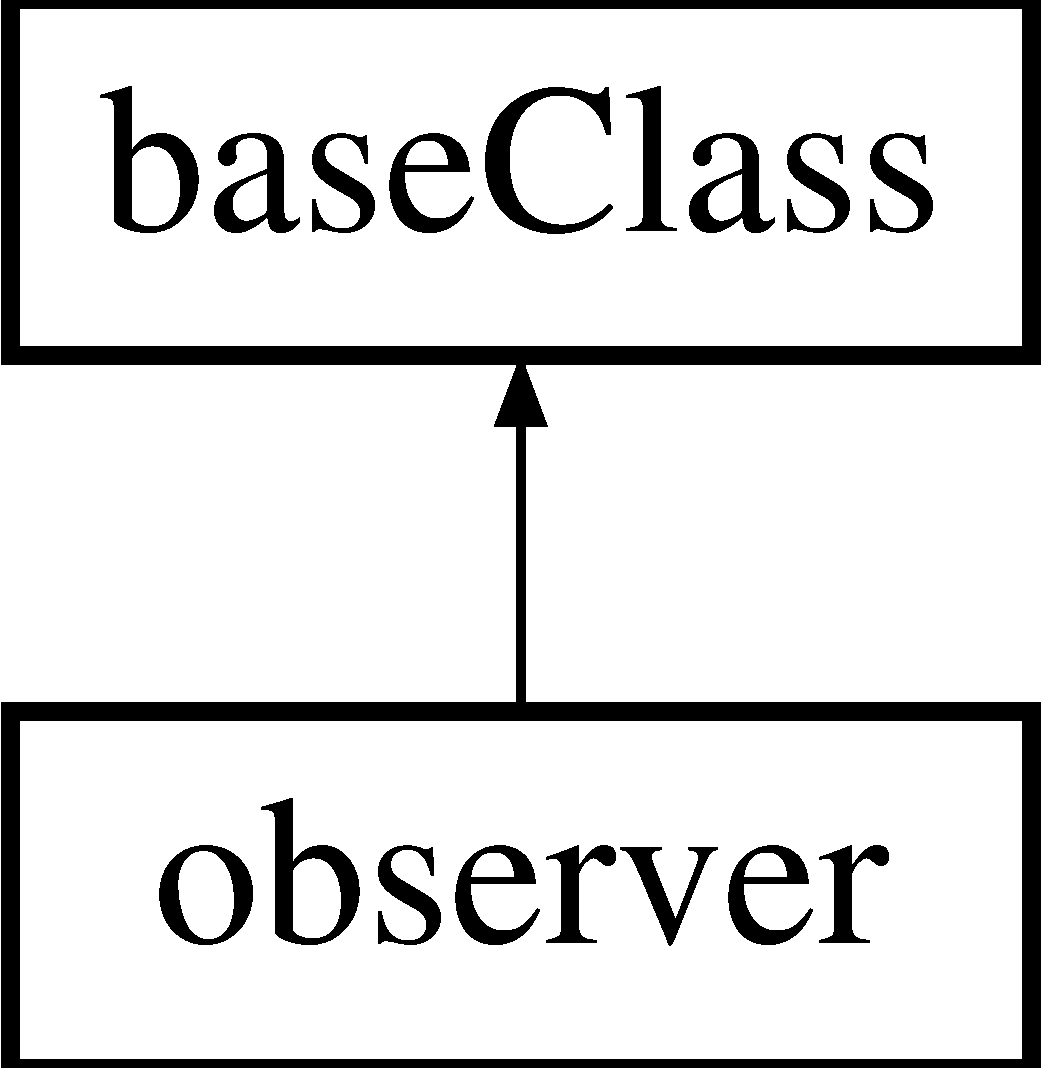
\includegraphics[height=2.000000cm]{classobserver}
\end{center}
\end{figure}


\subsection{Detailed Description}
Class is mainly used to calculate observed values from intrinsic jet properties such as observed luminosities instead of luminosities in jet co-\/moving frame or flare \subsection*{Public Member Functions}
\begin{DoxyCompactItemize}
\item 
\hyperlink{classobserver_a42314af9846ce37a6cdadd7a027eed12}{observer} (scfgp $\ast$\-\_\-cfg, \hyperlink{classjetGeometry}{jet\-Geometry} $\ast$\-\_\-r, std\-::string \-\_\-id)
\item 
\hyperlink{classobserver_acb64c4c8de3e36b5cce282dc139e602c}{$\sim$observer} ()
\item 
void \hyperlink{classobserver_a1fbeb6a33647dfadbb1ca9c0d64953bb}{print\-Info} ()
\item 
int \hyperlink{classobserver_aa28bd51f0a5bda86584ae35cd32603d6}{if\-Calculate\-Flares} ()
\item 
int \hyperlink{classobserver_af12e74dd21611778bc53e1766cbd4349}{get\-Freq\-List\-Size} ()
\item 
double \hyperlink{classobserver_a36e7c21680cd2ba038fb7cf3e6dfb77b}{get\-Freq\-List} (int i)
\item 
void \hyperlink{classobserver_a0e5aaaf485e52230ade3ebc034956608}{add\-En\-Diss\-Proc} (\hyperlink{classenergyDissProc}{energy\-Diss\-Proc} $\ast$\-\_\-obj)
\item 
void \hyperlink{classobserver_a0bfece68d09337e339436326fdf2eabc}{list\-En\-Diss\-Proc} ()
\item 
int \hyperlink{classobserver_a3455cd549f8a75cbe2f5c068ae88ec79}{size\-En\-Diss\-Proc} ()
\item 
void \hyperlink{classobserver_a9e6f78fade71b521003ee502c0eafaab}{add\-En\-Diss\-Proc\-Point} (\hyperlink{classenergyDissProc}{energy\-Diss\-Proc} $\ast$\-\_\-obj)
\item 
void \hyperlink{classobserver_ac92a23cc40135eff9c9d443becd9dfa2}{list\-En\-Diss\-Proc\-Point} ()
\item 
int \hyperlink{classobserver_ade865c5881df7e3fc884b50ca812c52e}{size\-En\-Diss\-Proc\-Point} ()
\item 
void \hyperlink{classobserver_a7755eb84eb5fc1bb7a5e84463034bf18}{add\-Ext\-Pl} (\hyperlink{classenergyDissProc}{energy\-Diss\-Proc} $\ast$\-\_\-obj)
\item 
void \hyperlink{classobserver_a86d811d98a5273c8e97444a2ac6606a1}{list\-Ext\-Pl} ()
\item 
int \hyperlink{classobserver_aa8290de1b8b9345c889ded609c7cd2d1}{size\-Ext\-Pl} ()
\item 
void \hyperlink{classobserver_a29d26dd051772217e0ca16b051ecd93f}{add\-Ext\-Sp} (\hyperlink{classenergyDissProc}{energy\-Diss\-Proc} $\ast$\-\_\-obj)
\item 
void \hyperlink{classobserver_aabb0a1a3fefbdb04844ae3555b13d038}{list\-Ext\-Sp} ()
\item 
int \hyperlink{classobserver_af0d03462bd4a837269c12d69f6b9199e}{size\-Ext\-Sp} ()
\item 
void \hyperlink{classobserver_a5f8d7efc385940222eb28d33378558b1}{add\-Ext\-Gu} (\hyperlink{classenergyDissProc}{energy\-Diss\-Proc} $\ast$\-\_\-obj)
\item 
void \hyperlink{classobserver_a06bd3a882a44a4bb4120aa18163a50f2}{list\-Ext\-Gu} ()
\item 
int \hyperlink{classobserver_ae0bf73a28d20debaa0066e4fbbac4395}{size\-Ext\-Gu} ()
\item 
void \hyperlink{classobserver_a341825cd835514e888203ffcf15ca5e6}{calculate\-Point\-Luminosity} (\hyperlink{classenergyDissProc}{energy\-Diss\-Proc} $\ast$\-\_\-obj)
\item 
void \hyperlink{classobserver_a2cdb4ba6523c5dbd3cb8383d4430a02f}{sum\-Point\-Luminosity} ()
\item 
void \hyperlink{classobserver_a78441d4287eb3e3991bfd8b19b74ef6e}{avg\-Point\-Luminosity} (\hyperlink{classenergyDissProc}{energy\-Diss\-Proc} $\ast$\-\_\-obj)
\item 
void \hyperlink{classobserver_a1906c04333220b8b121eda23e838fe63}{sum\-Point\-Avg\-Luminosity} ()
\item 
void \hyperlink{classobserver_ad34fc6b2013c4ce294c936c790747405}{add\-Q\-Accd\-Luminosity} (\hyperlink{classQuasarAccDisk}{Quasar\-Acc\-Disk} $\ast$Q\-Accd)
\item 
double \hyperlink{classobserver_a26080f0ca55ac7ae6f306bc11d18263d}{calculate\-Flare} (\hyperlink{classenergyDissProc}{energy\-Diss\-Proc} $\ast$\-\_\-obj, double nu)
\item 
void \hyperlink{classobserver_ade82015679a882a1052e6594dca46cb8}{calculate\-All\-Flares} ()
\item 
double \hyperlink{classobserver_af7fe35310b73997a7dab21cd6d4141db}{interpolate} (gsl\-\_\-vector $\ast$x, gsl\-\_\-vector $\ast$y, double x\-To\-Interpolate)
\item 
void \hyperlink{classobserver_a9b5776b8a4d70f92cc82630e30b7bfeb}{save\-Point\-Luminosity} (\hyperlink{classenergyDissProc}{energy\-Diss\-Proc} $\ast$x)
\item 
void \hyperlink{classobserver_a6785229b7211bfa2e161e6a27953caf3}{save\-Point\-Luminosity\-Sum} ()
\item 
void \hyperlink{classobserver_a339e054afe8cda7d6707b1b0f8c59127}{save\-Point\-Luminosity\-Sum} (gsl\-\_\-vector $\ast$gamma)
\item 
void \hyperlink{classobserver_aa01a0e777fe58f4b88dd80da83677a62}{save\-Averaged\-Point\-Luminosity} (\hyperlink{classenergyDissProc}{energy\-Diss\-Proc} $\ast$x)
\item 
void \hyperlink{classobserver_a779e4c80cec4aa433fcb204fe0043ed7}{save\-Averaged\-Point\-Luminosity\-Sum} ()
\item 
void \hyperlink{classobserver_a2e7b0b16db25865c6fd6f7ce251ffd5d}{save\-Averaged\-Point\-Luminosity\-Sum} (gsl\-\_\-vector $\ast$gamma)
\end{DoxyCompactItemize}
\subsection*{Public Attributes}
\begin{DoxyCompactItemize}
\item 
std\-::vector$<$ \hyperlink{classenergyDissProc}{energy\-Diss\-Proc} $\ast$ $>$ \hyperlink{classobserver_aeb5a8afa2221e268e06f74600acac7af}{En\-Diss\-Proc}
\item 
\hypertarget{classobserver_a18c7cc72d61f5610f8d56ec80c758251}{std\-::vector$<$ \hyperlink{classenergyDissProc}{energy\-Diss\-Proc} $\ast$ $>$ {\bfseries En\-Diss\-Proc\-Point}}\label{classobserver_a18c7cc72d61f5610f8d56ec80c758251}

\item 
\hypertarget{classobserver_ab825bcea700d3d9cb6dfba26edcda166}{std\-::vector$<$ \hyperlink{classenergyDissProc}{energy\-Diss\-Proc} $\ast$ $>$ {\bfseries Ext\-Pl}}\label{classobserver_ab825bcea700d3d9cb6dfba26edcda166}

\item 
\hypertarget{classobserver_a1d6a26b2cbfc866024c762525a048aaf}{std\-::vector$<$ \hyperlink{classenergyDissProc}{energy\-Diss\-Proc} $\ast$ $>$ {\bfseries Ext\-Sp}}\label{classobserver_a1d6a26b2cbfc866024c762525a048aaf}

\item 
\hypertarget{classobserver_ac69c17944b5eef96e875afc47f07f363}{std\-::vector$<$ \hyperlink{classenergyDissProc}{energy\-Diss\-Proc} $\ast$ $>$ {\bfseries Ext\-Gu}}\label{classobserver_ac69c17944b5eef96e875afc47f07f363}

\item 
gsl\-\_\-vector $\ast$ \hyperlink{classobserver_aef3c4770dc82fdb0d2ac7143e184cbc3}{v\-Point\-Sum}
\item 
\hypertarget{classobserver_a57f1a467bfc7855bec6b6ce971cc7c7e}{gsl\-\_\-vector $\ast$ {\bfseries Lv\-Point\-Sum}}\label{classobserver_a57f1a467bfc7855bec6b6ce971cc7c7e}

\item 
\hypertarget{classobserver_a1894b3a158640b8c93d6de5ce72cb775}{gsl\-\_\-vector $\ast$ {\bfseries Lv\-Point\-Avg\-Sum}}\label{classobserver_a1894b3a158640b8c93d6de5ce72cb775}

\item 
std\-::vector$<$ double $>$ \hyperlink{classobserver_a64f3e868a83ea1c693a329aba1f83560}{freq\-List}
\end{DoxyCompactItemize}


\subsection{Constructor \& Destructor Documentation}
\hypertarget{classobserver_a42314af9846ce37a6cdadd7a027eed12}{\index{observer@{observer}!observer@{observer}}
\index{observer@{observer}!observer@{observer}}
\subsubsection[{observer}]{\setlength{\rightskip}{0pt plus 5cm}observer\-::observer (
\begin{DoxyParamCaption}
\item[{scfgp $\ast$}]{\-\_\-cfg, }
\item[{{\bf jet\-Geometry} $\ast$}]{\-\_\-r, }
\item[{std\-::string}]{\-\_\-id}
\end{DoxyParamCaption}
)}}\label{classobserver_a42314af9846ce37a6cdadd7a027eed12}
constructor 
\begin{DoxyParams}{Parameters}
{\em scfgp} & \\
\hline
{\em jetgeometry} & \\
\hline
{\em id} & \\
\hline
\end{DoxyParams}

\begin{DoxyCode}
10                                                                 : \hyperlink{classbaseClass}{baseClass}(\_cfg, \_r, \_id ) \{ 
11   \textcolor{comment}{/* request parameters */}
12   \hyperlink{classbaseClass_a744f87a6ebe63da08256c022d42a4ca7}{cfg} -> request<int>(\textcolor{stringliteral}{"N"}+\hyperlink{classbaseClass_a4d5ff386a69bcbe21b5976f55b624df6}{id},1000,&\hyperlink{classbaseClass_a2b4d07d2b46197d495de0477f4bb22f8}{N});
13   \hyperlink{classbaseClass_a744f87a6ebe63da08256c022d42a4ca7}{cfg} -> request<double>(\textcolor{stringliteral}{"thetaObs"},0.1,&thetaObs);
14   \hyperlink{classbaseClass_a744f87a6ebe63da08256c022d42a4ca7}{cfg} -> request<double>(\textcolor{stringliteral}{"thetaJ"},0.1,&thetaJ);
15   \hyperlink{classbaseClass_a744f87a6ebe63da08256c022d42a4ca7}{cfg} -> request<double>(\textcolor{stringliteral}{"nu1"},0,&nu1);
16   \hyperlink{classbaseClass_a744f87a6ebe63da08256c022d42a4ca7}{cfg} -> request<double>(\textcolor{stringliteral}{"nu2"},0,&nu2);
17   \hyperlink{classbaseClass_a744f87a6ebe63da08256c022d42a4ca7}{cfg} -> request<double>(\textcolor{stringliteral}{"nu3"},0,&nu3);
18   \hyperlink{classbaseClass_a744f87a6ebe63da08256c022d42a4ca7}{cfg} -> request<double>(\textcolor{stringliteral}{"nu4"},0,&nu4);
19   \hyperlink{classbaseClass_a744f87a6ebe63da08256c022d42a4ca7}{cfg} -> request<double>(\textcolor{stringliteral}{"nu5"},0,&nu5);
20   \hyperlink{classbaseClass_a744f87a6ebe63da08256c022d42a4ca7}{cfg} -> request<double>(\textcolor{stringliteral}{"nu6"},0,&nu6);
21   \hyperlink{classbaseClass_a744f87a6ebe63da08256c022d42a4ca7}{cfg} -> request<double>(\textcolor{stringliteral}{"Gamma"},10.0,&Gamma);
22   \hyperlink{classbaseClass_a744f87a6ebe63da08256c022d42a4ca7}{cfg} -> request<std::string>(\textcolor{stringliteral}{"lumModel"},\textcolor{stringliteral}{"blob"},&lumModel);
23   \hyperlink{classbaseClass_a744f87a6ebe63da08256c022d42a4ca7}{cfg} -> request<int>(\textcolor{stringliteral}{"saveLumPoint"},0,&saveLumPoint);
24   \hyperlink{classbaseClass_a744f87a6ebe63da08256c022d42a4ca7}{cfg} -> request<int>(\textcolor{stringliteral}{"saveLumPointAvg"},0,&saveLumPointAvg);
25   \hyperlink{classbaseClass_a744f87a6ebe63da08256c022d42a4ca7}{cfg} -> request<int>(\textcolor{stringliteral}{"saveExtPlVsRm"},0,&saveExtPlVsRm);
26 
27   \hyperlink{classbaseClass_a744f87a6ebe63da08256c022d42a4ca7}{cfg} -> updateRequests( );
28   
29   allocateLvPointSum( );
30   allocateLvPointAvgSum( ); \}
\end{DoxyCode}
\hypertarget{classobserver_acb64c4c8de3e36b5cce282dc139e602c}{\index{observer@{observer}!$\sim$observer@{$\sim$observer}}
\index{$\sim$observer@{$\sim$observer}!observer@{observer}}
\subsubsection[{$\sim$observer}]{\setlength{\rightskip}{0pt plus 5cm}observer\-::$\sim$observer (
\begin{DoxyParamCaption}
{}
\end{DoxyParamCaption}
)}}\label{classobserver_acb64c4c8de3e36b5cce282dc139e602c}
destructor 
\begin{DoxyCode}
32                      \{
33   freeLvPointSum( );
34   freeLvPointAvgSum( ); \}
\end{DoxyCode}


\subsection{Member Function Documentation}
\hypertarget{classobserver_a0e5aaaf485e52230ade3ebc034956608}{\index{observer@{observer}!add\-En\-Diss\-Proc@{add\-En\-Diss\-Proc}}
\index{add\-En\-Diss\-Proc@{add\-En\-Diss\-Proc}!observer@{observer}}
\subsubsection[{add\-En\-Diss\-Proc}]{\setlength{\rightskip}{0pt plus 5cm}void observer\-::add\-En\-Diss\-Proc (
\begin{DoxyParamCaption}
\item[{{\bf energy\-Diss\-Proc} $\ast$}]{\-\_\-obj}
\end{DoxyParamCaption}
)}}\label{classobserver_a0e5aaaf485e52230ade3ebc034956608}
add energy dissipation process to list of active ones 
\begin{DoxyParams}{Parameters}
{\em \hyperlink{classenergyDissProc}{energy\-Diss\-Proc}} & \\
\hline
\end{DoxyParams}

\begin{DoxyCode}
79 \{ \hyperlink{classobserver_aeb5a8afa2221e268e06f74600acac7af}{EnDissProc}.push\_back( \_obj ); \}
\end{DoxyCode}
\hypertarget{classobserver_a9e6f78fade71b521003ee502c0eafaab}{\index{observer@{observer}!add\-En\-Diss\-Proc\-Point@{add\-En\-Diss\-Proc\-Point}}
\index{add\-En\-Diss\-Proc\-Point@{add\-En\-Diss\-Proc\-Point}!observer@{observer}}
\subsubsection[{add\-En\-Diss\-Proc\-Point}]{\setlength{\rightskip}{0pt plus 5cm}void observer\-::add\-En\-Diss\-Proc\-Point (
\begin{DoxyParamCaption}
\item[{{\bf energy\-Diss\-Proc} $\ast$}]{\-\_\-obj}
\end{DoxyParamCaption}
)}}\label{classobserver_a9e6f78fade71b521003ee502c0eafaab}
add energy dissipation process to list of those for which we have to calculate 'point source' luminosity 
\begin{DoxyParams}{Parameters}
{\em \hyperlink{classenergyDissProc}{energy\-Diss\-Proc}} & \\
\hline
\end{DoxyParams}

\begin{DoxyCode}
80 \{ EnDissProcPoint.push\_back( \_obj ); \}
\end{DoxyCode}
\hypertarget{classobserver_a5f8d7efc385940222eb28d33378558b1}{\index{observer@{observer}!add\-Ext\-Gu@{add\-Ext\-Gu}}
\index{add\-Ext\-Gu@{add\-Ext\-Gu}!observer@{observer}}
\subsubsection[{add\-Ext\-Gu}]{\setlength{\rightskip}{0pt plus 5cm}void observer\-::add\-Ext\-Gu (
\begin{DoxyParamCaption}
\item[{{\bf energy\-Diss\-Proc} $\ast$}]{\-\_\-obj}
\end{DoxyParamCaption}
)}}\label{classobserver_a5f8d7efc385940222eb28d33378558b1}
add Ext\-Gu process to list of active ones 
\begin{DoxyParams}{Parameters}
{\em \hyperlink{classenergyDissProc}{energy\-Diss\-Proc}} & \\
\hline
\end{DoxyParams}

\begin{DoxyCode}
83 \{ ExtGu.push\_back( \_obj ); \}
\end{DoxyCode}
\hypertarget{classobserver_a7755eb84eb5fc1bb7a5e84463034bf18}{\index{observer@{observer}!add\-Ext\-Pl@{add\-Ext\-Pl}}
\index{add\-Ext\-Pl@{add\-Ext\-Pl}!observer@{observer}}
\subsubsection[{add\-Ext\-Pl}]{\setlength{\rightskip}{0pt plus 5cm}void observer\-::add\-Ext\-Pl (
\begin{DoxyParamCaption}
\item[{{\bf energy\-Diss\-Proc} $\ast$}]{\-\_\-obj}
\end{DoxyParamCaption}
)}}\label{classobserver_a7755eb84eb5fc1bb7a5e84463034bf18}
add Ext\-Pl process to list of active ones 
\begin{DoxyParams}{Parameters}
{\em \hyperlink{classenergyDissProc}{energy\-Diss\-Proc}} & \\
\hline
\end{DoxyParams}

\begin{DoxyCode}
81 \{ ExtPl.push\_back( \_obj ); \}
\end{DoxyCode}
\hypertarget{classobserver_a29d26dd051772217e0ca16b051ecd93f}{\index{observer@{observer}!add\-Ext\-Sp@{add\-Ext\-Sp}}
\index{add\-Ext\-Sp@{add\-Ext\-Sp}!observer@{observer}}
\subsubsection[{add\-Ext\-Sp}]{\setlength{\rightskip}{0pt plus 5cm}void observer\-::add\-Ext\-Sp (
\begin{DoxyParamCaption}
\item[{{\bf energy\-Diss\-Proc} $\ast$}]{\-\_\-obj}
\end{DoxyParamCaption}
)}}\label{classobserver_a29d26dd051772217e0ca16b051ecd93f}
add Ext\-Sp process to list of active ones 
\begin{DoxyParams}{Parameters}
{\em \hyperlink{classenergyDissProc}{energy\-Diss\-Proc}} & \\
\hline
\end{DoxyParams}

\begin{DoxyCode}
82 \{ ExtSp.push\_back( \_obj ); \}
\end{DoxyCode}
\hypertarget{classobserver_ad34fc6b2013c4ce294c936c790747405}{\index{observer@{observer}!add\-Q\-Accd\-Luminosity@{add\-Q\-Accd\-Luminosity}}
\index{add\-Q\-Accd\-Luminosity@{add\-Q\-Accd\-Luminosity}!observer@{observer}}
\subsubsection[{add\-Q\-Accd\-Luminosity}]{\setlength{\rightskip}{0pt plus 5cm}void observer\-::add\-Q\-Accd\-Luminosity (
\begin{DoxyParamCaption}
\item[{{\bf Quasar\-Acc\-Disk} $\ast$}]{Q\-Accd}
\end{DoxyParamCaption}
)}}\label{classobserver_ad34fc6b2013c4ce294c936c790747405}
add Quasar Template to calculated luminosities 
\begin{DoxyParams}{Parameters}
{\em \hyperlink{classQuasarAccDisk}{Quasar\-Acc\-Disk}} & \\
\hline
\end{DoxyParams}

\begin{DoxyCode}
171                                                         \{
172   bazinga::info(\textcolor{keywordtype}{id},\textcolor{stringliteral}{"Adding QAccd spectra to averaged point source luminosities ..."});
173 
174   \textcolor{keywordtype}{double} QAccd\_vmin = gsl\_vector\_min( QAccd -> vTemplate );
175   \textcolor{keywordtype}{double} QAccd\_vmax = gsl\_vector\_max( QAccd -> vTemplate );
176   bazinga::print\_info(\textcolor{keywordtype}{id}, \textcolor{stringliteral}{"QAccd vmin"}, QAccd\_vmin );
177   bazinga::print\_info(\textcolor{keywordtype}{id}, \textcolor{stringliteral}{"QAccd vmax"}, QAccd\_vmax );
178 
179   \textcolor{keywordtype}{double} interpolatedValue = 0.0;
180   \textcolor{keywordflow}{for}( \textcolor{keywordtype}{int} i=0;i<\hyperlink{classbaseClass_a2b4d07d2b46197d495de0477f4bb22f8}{N};i++ ) \{
181     interpolatedValue = gsl\_vector\_get( LvPointAvgSum, i );
182     \textcolor{keywordflow}{if}( gsl\_vector\_get( \hyperlink{classobserver_aef3c4770dc82fdb0d2ac7143e184cbc3}{vPointSum}, i ) > QAccd\_vmin && gsl\_vector\_get( 
      \hyperlink{classobserver_aef3c4770dc82fdb0d2ac7143e184cbc3}{vPointSum}, i ) < QAccd\_vmax )
183       interpolatedValue += \hyperlink{classobserver_af7fe35310b73997a7dab21cd6d4141db}{interpolate}( QAccd -> vTemplate, QAccd -> LvTemplate, gsl\_vector\_get(
       \hyperlink{classobserver_aef3c4770dc82fdb0d2ac7143e184cbc3}{vPointSum}, i ) );
184     
185     gsl\_vector\_set( LvPointAvgSum, i, interpolatedValue );
186   \}
187 \}
\end{DoxyCode}
\hypertarget{classobserver_a78441d4287eb3e3991bfd8b19b74ef6e}{\index{observer@{observer}!avg\-Point\-Luminosity@{avg\-Point\-Luminosity}}
\index{avg\-Point\-Luminosity@{avg\-Point\-Luminosity}!observer@{observer}}
\subsubsection[{avg\-Point\-Luminosity}]{\setlength{\rightskip}{0pt plus 5cm}void observer\-::avg\-Point\-Luminosity (
\begin{DoxyParamCaption}
\item[{{\bf energy\-Diss\-Proc} $\ast$}]{\-\_\-obj}
\end{DoxyParamCaption}
)}}\label{classobserver_a78441d4287eb3e3991bfd8b19b74ef6e}
calculate averaged 'point-\/source' luminosity; avergaed over all s-\/cells in the jet avtive region 
\begin{DoxyParams}{Parameters}
{\em \hyperlink{classenergyDissProc}{energy\-Diss\-Proc}} & \\
\hline
\end{DoxyParams}

\begin{DoxyCode}
125                                                      \{
126   bazinga::info(\textcolor{keywordtype}{id},\textcolor{stringliteral}{"Averaging spectra"}, x -> \hyperlink{classbaseClass_a756d5accf10ced9a34024048c95a51c9}{whoAmI}( ) );
127   \textcolor{keywordflow}{for}( \textcolor{keywordtype}{int} i=0;i<x->N;i++ ) \{
128     \textcolor{keywordflow}{if}( lumModel == \textcolor{stringliteral}{"blob"} ) \{ x->set\_LvPointAvg( i, x->get\_LvPointAvg( i ) + x->get\_LvPoint( i )/
      \hyperlink{classbaseClass_a482bb9b1d94f3eb3f31026d14e9a2bb6}{r}->getNinj( ) ); \}
129     \textcolor{keywordflow}{if}( lumModel == \textcolor{stringliteral}{"steady"} ) \{ x->set\_LvPointAvg( i, x->get\_LvPointAvg( i ) + x->get\_LvPoint( i ) ); \}
130   \}
131 \}
\end{DoxyCode}
\hypertarget{classobserver_ade82015679a882a1052e6594dca46cb8}{\index{observer@{observer}!calculate\-All\-Flares@{calculate\-All\-Flares}}
\index{calculate\-All\-Flares@{calculate\-All\-Flares}!observer@{observer}}
\subsubsection[{calculate\-All\-Flares}]{\setlength{\rightskip}{0pt plus 5cm}void observer\-::calculate\-All\-Flares (
\begin{DoxyParamCaption}
{}
\end{DoxyParamCaption}
)}}\label{classobserver_ade82015679a882a1052e6594dca46cb8}
calculate all flares 
\begin{DoxyCode}
40                                    \{
41   \textcolor{keywordflow}{if}( nu1 || nu2 || nu3 || nu4 || nu5 || nu6 ) \{
42     bazinga::info(\textcolor{keywordtype}{id},\textcolor{stringliteral}{"Calculating flares"});
43     \textcolor{keywordflow}{for}( \textcolor{keywordtype}{int} j=0; j<\hyperlink{classobserver_ade865c5881df7e3fc884b50ca812c52e}{sizeEnDissProcPoint}(); j++ ) \{
44       bazinga::info(\textcolor{keywordtype}{id},\textcolor{stringliteral}{"Calculating point source flare"},EnDissProcPoint[j]->
      \hyperlink{classbaseClass_a756d5accf10ced9a34024048c95a51c9}{whoAmI}( ));
45       \textcolor{keywordflow}{for}( \textcolor{keywordtype}{int} k=0; k<\hyperlink{classobserver_af12e74dd21611778bc53e1766cbd4349}{getFreqListSize}(); k++ ) \{
46     \hyperlink{classobserver_a26080f0ca55ac7ae6f306bc11d18263d}{calculateFlare}( \hyperlink{classobserver_aeb5a8afa2221e268e06f74600acac7af}{EnDissProc}[j], \hyperlink{classobserver_a36e7c21680cd2ba038fb7cf3e6dfb77b}{getFreqList}(k) );
47     bazinga::print\_info(\textcolor{keywordtype}{id},\textcolor{stringliteral}{"frequency"},\hyperlink{classobserver_a36e7c21680cd2ba038fb7cf3e6dfb77b}{getFreqList}(k),\textcolor{stringliteral}{"Hz"}); \}
48     \}
49   \}
50 \}
\end{DoxyCode}
\hypertarget{classobserver_a26080f0ca55ac7ae6f306bc11d18263d}{\index{observer@{observer}!calculate\-Flare@{calculate\-Flare}}
\index{calculate\-Flare@{calculate\-Flare}!observer@{observer}}
\subsubsection[{calculate\-Flare}]{\setlength{\rightskip}{0pt plus 5cm}double observer\-::calculate\-Flare (
\begin{DoxyParamCaption}
\item[{{\bf energy\-Diss\-Proc} $\ast$}]{\-\_\-obj, }
\item[{double}]{nu}
\end{DoxyParamCaption}
)}}\label{classobserver_a26080f0ca55ac7ae6f306bc11d18263d}
calculate flares 
\begin{DoxyParams}{Parameters}
{\em \hyperlink{classenergyDissProc}{energy\-Diss\-Proc}} & \\
\hline
{\em frequency} & \\
\hline
\end{DoxyParams}

\begin{DoxyCode}
229                                                                 \{
230   gsl\_vector* temp\_x = gsl\_vector\_alloc( obj->N );
231   gsl\_vector* temp\_y = gsl\_vector\_alloc( obj->N );
232   
233   gsl\_vector* rad = gsl\_vector\_alloc( \hyperlink{classbaseClass_a482bb9b1d94f3eb3f31026d14e9a2bb6}{r}->getMaxIndex() );
234   gsl\_vector* flare = gsl\_vector\_alloc( \hyperlink{classbaseClass_a482bb9b1d94f3eb3f31026d14e9a2bb6}{r}->getMaxIndex() );
235   
236   \textcolor{keywordflow}{for}( \textcolor{keywordtype}{int} i=0;i<\hyperlink{classbaseClass_a482bb9b1d94f3eb3f31026d14e9a2bb6}{r}->getMaxIndex();i++ ) \{
237     gsl\_vector\_set\_zero( temp\_x );
238     gsl\_vector\_set\_zero( temp\_y );
239     
240     \hyperlink{classbaseClass_a482bb9b1d94f3eb3f31026d14e9a2bb6}{r}->update( i );
241       
242     gsl\_vector\_memcpy( temp\_x, obj->vPoint );
243     gsl\_vector\_memcpy( temp\_y, obj->LvPoint );
244     gsl\_vector\_mul( temp\_y, temp\_x );
245     
246     gsl\_vector\_set( rad, i, \hyperlink{classbaseClass_a482bb9b1d94f3eb3f31026d14e9a2bb6}{r}->get() );
247     gsl\_vector\_set( flare, i, \hyperlink{classobserver_af7fe35310b73997a7dab21cd6d4141db}{interpolate}( temp\_x, temp\_y, nu ) ); \}
248   
249   std::string type = \textcolor{stringliteral}{"FlarePoint\_"};
250   type += obj->whoAmI( );
251   bazinga::info(\textcolor{keywordtype}{id},\textcolor{stringliteral}{"Saving flare."});
252   bazinga::save\_GSLVectorFlare( type, \hyperlink{classbaseClass_a482bb9b1d94f3eb3f31026d14e9a2bb6}{r}->getRadius\_GSLVector( ), flare, nu, \hyperlink{classbaseClass_a744f87a6ebe63da08256c022d42a4ca7}{cfg}->get<std::string>(\textcolor{stringliteral}{"
      output"}) );
253 
254   gsl\_vector\_free( temp\_x );
255   gsl\_vector\_free( temp\_y );
256   
257   gsl\_vector\_free( rad );
258   gsl\_vector\_free( flare ); \}
\end{DoxyCode}
\hypertarget{classobserver_a341825cd835514e888203ffcf15ca5e6}{\index{observer@{observer}!calculate\-Point\-Luminosity@{calculate\-Point\-Luminosity}}
\index{calculate\-Point\-Luminosity@{calculate\-Point\-Luminosity}!observer@{observer}}
\subsubsection[{calculate\-Point\-Luminosity}]{\setlength{\rightskip}{0pt plus 5cm}void observer\-::calculate\-Point\-Luminosity (
\begin{DoxyParamCaption}
\item[{{\bf energy\-Diss\-Proc} $\ast$}]{\-\_\-obj}
\end{DoxyParamCaption}
)}}\label{classobserver_a341825cd835514e888203ffcf15ca5e6}
caluclate 'point-\/source' luminosity 
\begin{DoxyParams}{Parameters}
{\em \hyperlink{classenergyDissProc}{energy\-Diss\-Proc}} & \\
\hline
\end{DoxyParams}

\begin{DoxyCode}
115                                                            \{
116   bazinga::info(\textcolor{keywordtype}{id},\textcolor{stringliteral}{"Calculating point source luminosity"}, x -> \hyperlink{classbaseClass_a756d5accf10ced9a34024048c95a51c9}{whoAmI}( ) );
117   \textcolor{keywordtype}{double} Doppler = 1.0/(Gamma*(1.0-cos( thetaObs )*\hyperlink{classbaseClass_a208facecf3a4480b47bebfce91413a39}{beta}(Gamma)));
118   \textcolor{keywordflow}{for}( \textcolor{keywordtype}{int} i=0;i<x->N;i++ ) \{
119     x->set\_vPoint( i, x->get\_vp( i )*Doppler );
120     \textcolor{keywordflow}{if}( lumModel == \textcolor{stringliteral}{"blob"} ) \{ x->set\_LvPoint( i, x->get\_Lpv( i )*pow(Doppler, 3) ); \}
121     \textcolor{keywordflow}{if}( lumModel == \textcolor{stringliteral}{"steady"} ) \{ x->set\_LvPoint( i, x->get\_Lpv( i )*pow(Doppler, 2)/Gamma ); \}
122   \}
123 \}
\end{DoxyCode}
\hypertarget{classobserver_a36e7c21680cd2ba038fb7cf3e6dfb77b}{\index{observer@{observer}!get\-Freq\-List@{get\-Freq\-List}}
\index{get\-Freq\-List@{get\-Freq\-List}!observer@{observer}}
\subsubsection[{get\-Freq\-List}]{\setlength{\rightskip}{0pt plus 5cm}double observer\-::get\-Freq\-List (
\begin{DoxyParamCaption}
\item[{int}]{i}
\end{DoxyParamCaption}
)}}\label{classobserver_a36e7c21680cd2ba038fb7cf3e6dfb77b}
get frequency 
\begin{DoxyParams}{Parameters}
{\em index} & \\
\hline
\end{DoxyParams}
\begin{DoxyReturn}{Returns}
i-\/th frequency 
\end{DoxyReturn}

\begin{DoxyCode}
38 \{ \textcolor{keywordflow}{return} \hyperlink{classobserver_a64f3e868a83ea1c693a329aba1f83560}{freqList}[i]; \}
\end{DoxyCode}
\hypertarget{classobserver_af12e74dd21611778bc53e1766cbd4349}{\index{observer@{observer}!get\-Freq\-List\-Size@{get\-Freq\-List\-Size}}
\index{get\-Freq\-List\-Size@{get\-Freq\-List\-Size}!observer@{observer}}
\subsubsection[{get\-Freq\-List\-Size}]{\setlength{\rightskip}{0pt plus 5cm}int observer\-::get\-Freq\-List\-Size (
\begin{DoxyParamCaption}
{}
\end{DoxyParamCaption}
)}}\label{classobserver_af12e74dd21611778bc53e1766cbd4349}
check how many frequencies to look at wen calculating flares \begin{DoxyReturn}{Returns}
number of frequencies 
\end{DoxyReturn}

\begin{DoxyCode}
36 \{ \textcolor{keywordflow}{return} \hyperlink{classobserver_a64f3e868a83ea1c693a329aba1f83560}{freqList}.size(); \}
\end{DoxyCode}
\hypertarget{classobserver_aa28bd51f0a5bda86584ae35cd32603d6}{\index{observer@{observer}!if\-Calculate\-Flares@{if\-Calculate\-Flares}}
\index{if\-Calculate\-Flares@{if\-Calculate\-Flares}!observer@{observer}}
\subsubsection[{if\-Calculate\-Flares}]{\setlength{\rightskip}{0pt plus 5cm}int observer\-::if\-Calculate\-Flares (
\begin{DoxyParamCaption}
{}
\end{DoxyParamCaption}
)}}\label{classobserver_aa28bd51f0a5bda86584ae35cd32603d6}
check if you should calculate flares \begin{DoxyReturn}{Returns}
1 if yes, 0 if no 
\end{DoxyReturn}

\begin{DoxyCode}
357                                  \{
358   \textcolor{keywordflow}{if}( nu1 || nu2 || nu3 || nu4 || nu5 || nu6 ) \{ \textcolor{keywordflow}{return} 1; \}
359   \textcolor{keywordflow}{else} \{ \textcolor{keywordflow}{return} 0; \}
360 \}
\end{DoxyCode}
\hypertarget{classobserver_af7fe35310b73997a7dab21cd6d4141db}{\index{observer@{observer}!interpolate@{interpolate}}
\index{interpolate@{interpolate}!observer@{observer}}
\subsubsection[{interpolate}]{\setlength{\rightskip}{0pt plus 5cm}double observer\-::interpolate (
\begin{DoxyParamCaption}
\item[{gsl\-\_\-vector $\ast$}]{x, }
\item[{gsl\-\_\-vector $\ast$}]{y, }
\item[{double}]{x\-To\-Interpolate}
\end{DoxyParamCaption}
)}}\label{classobserver_af7fe35310b73997a7dab21cd6d4141db}
technical\-: interpolate data y( x ) 
\begin{DoxyParams}{Parameters}
{\em gsl\-\_\-vector} & x \\
\hline
{\em gsl\-\_\-vector} & y \\
\hline
{\em x\-\_\-value} & to calculate y( x\-\_\-value ) \\
\hline
\end{DoxyParams}

\begin{DoxyCode}
260                                                                       \{
261   \textcolor{keywordtype}{double} interpolatedValue;
262   \textcolor{keywordtype}{double} xmin, xmax = 0.0;
263   
264   \textcolor{keywordflow}{if}( \_x < gsl\_vector\_min( x ) || \_x > gsl\_vector\_max( x ) ) \{ interpolatedValue = 1.0; \}
265   
266   \textcolor{keywordflow}{for}( \textcolor{keywordtype}{int} i=0; i<x->size-1; i++ ) \{
267     \textcolor{keywordflow}{if}( gsl\_vector\_get( x, i ) > \_x ) \{
268       \textcolor{keywordflow}{if}( gsl\_vector\_get( y, i ) == 0 || gsl\_vector\_get( y, i+1 ) == 0 ) \{ interpolatedValue = 0.0; \}
269       \textcolor{keywordflow}{else} \{
270     interpolatedValue = log( gsl\_vector\_get( y, i ) ) + log(gsl\_vector\_get( y, i+1 )/gsl\_vector\_get( y, i )
      )/log(gsl\_vector\_get( x, i+1 )/gsl\_vector\_get( x, i ))*log(\_x/gsl\_vector\_get( x, i ) );
271       \}
272       interpolatedValue = exp(interpolatedValue);
273       \textcolor{comment}{//      interpolatedValue = 0.5*( gsl\_vector\_get( y, i ) + gsl\_vector\_get( y, i+1 ) );}
274       \textcolor{keywordflow}{break}; \}
275   \}   
276 
277   \textcolor{keywordflow}{return} interpolatedValue; \}
\end{DoxyCode}
\hypertarget{classobserver_a0bfece68d09337e339436326fdf2eabc}{\index{observer@{observer}!list\-En\-Diss\-Proc@{list\-En\-Diss\-Proc}}
\index{list\-En\-Diss\-Proc@{list\-En\-Diss\-Proc}!observer@{observer}}
\subsubsection[{list\-En\-Diss\-Proc}]{\setlength{\rightskip}{0pt plus 5cm}void observer\-::list\-En\-Diss\-Proc (
\begin{DoxyParamCaption}
{}
\end{DoxyParamCaption}
)}}\label{classobserver_a0bfece68d09337e339436326fdf2eabc}
show active energy dissipation processes 
\begin{DoxyCode}
105                                \{
106   std::stringstream s;
107   \textcolor{keywordflow}{for}( \textcolor{keywordtype}{int} i=0; i<\hyperlink{classobserver_aeb5a8afa2221e268e06f74600acac7af}{EnDissProc}.size(); i++ ) s << \hyperlink{classobserver_aeb5a8afa2221e268e06f74600acac7af}{EnDissProc}[i]->
      \hyperlink{classbaseClass_a756d5accf10ced9a34024048c95a51c9}{whoAmI}() << \textcolor{stringliteral}{" "};
108   bazinga::print\_info(\textcolor{keywordtype}{id},\textcolor{stringliteral}{"Processes used to calculate intrinsic lumonisities"},s.str()); \}
\end{DoxyCode}
\hypertarget{classobserver_ac92a23cc40135eff9c9d443becd9dfa2}{\index{observer@{observer}!list\-En\-Diss\-Proc\-Point@{list\-En\-Diss\-Proc\-Point}}
\index{list\-En\-Diss\-Proc\-Point@{list\-En\-Diss\-Proc\-Point}!observer@{observer}}
\subsubsection[{list\-En\-Diss\-Proc\-Point}]{\setlength{\rightskip}{0pt plus 5cm}void observer\-::list\-En\-Diss\-Proc\-Point (
\begin{DoxyParamCaption}
{}
\end{DoxyParamCaption}
)}}\label{classobserver_ac92a23cc40135eff9c9d443becd9dfa2}
show active energy dissipation processes for which we have to calculate 'point source' luminosity 
\begin{DoxyCode}
110                                     \{
111   std::stringstream s;
112   \textcolor{keywordflow}{for}( \textcolor{keywordtype}{int} i=0; i<EnDissProcPoint.size(); i++ ) s << EnDissProcPoint[i]->\hyperlink{classbaseClass_a756d5accf10ced9a34024048c95a51c9}{whoAmI}() << \textcolor{stringliteral}{" "};
113   bazinga::print\_info(\textcolor{keywordtype}{id},\textcolor{stringliteral}{"Processes used to calculate point lumonisities"},s.str()); \}
\end{DoxyCode}
\hypertarget{classobserver_a06bd3a882a44a4bb4120aa18163a50f2}{\index{observer@{observer}!list\-Ext\-Gu@{list\-Ext\-Gu}}
\index{list\-Ext\-Gu@{list\-Ext\-Gu}!observer@{observer}}
\subsubsection[{list\-Ext\-Gu}]{\setlength{\rightskip}{0pt plus 5cm}void observer\-::list\-Ext\-Gu (
\begin{DoxyParamCaption}
{}
\end{DoxyParamCaption}
)}}\label{classobserver_a06bd3a882a44a4bb4120aa18163a50f2}
show active Ext\-Gu energy dissipation processes 
\begin{DoxyCode}
100                           \{
101   std::stringstream s;
102   \textcolor{keywordflow}{for}( \textcolor{keywordtype}{int} i=0; i<ExtGu.size(); i++ ) s << ExtGu[i]->\hyperlink{classbaseClass_a756d5accf10ced9a34024048c95a51c9}{whoAmI}() << \textcolor{stringliteral}{" "};
103   bazinga::print\_info(\textcolor{keywordtype}{id},\textcolor{stringliteral}{"External Radiation Gu Sources"},s.str()); \}
\end{DoxyCode}
\hypertarget{classobserver_a86d811d98a5273c8e97444a2ac6606a1}{\index{observer@{observer}!list\-Ext\-Pl@{list\-Ext\-Pl}}
\index{list\-Ext\-Pl@{list\-Ext\-Pl}!observer@{observer}}
\subsubsection[{list\-Ext\-Pl}]{\setlength{\rightskip}{0pt plus 5cm}void observer\-::list\-Ext\-Pl (
\begin{DoxyParamCaption}
{}
\end{DoxyParamCaption}
)}}\label{classobserver_a86d811d98a5273c8e97444a2ac6606a1}
show active Ext\-Pl energy dissipation processes 
\begin{DoxyCode}
90                           \{
91   std::stringstream s;
92   \textcolor{keywordflow}{for}( \textcolor{keywordtype}{int} i=0; i<ExtPl.size(); i++ ) s << ExtPl[i]->\hyperlink{classbaseClass_a756d5accf10ced9a34024048c95a51c9}{whoAmI}() << \textcolor{stringliteral}{" "};
93   bazinga::print\_info(\textcolor{keywordtype}{id},\textcolor{stringliteral}{"External Radiation Planar Sources"},s.str()); \}
\end{DoxyCode}
\hypertarget{classobserver_aabb0a1a3fefbdb04844ae3555b13d038}{\index{observer@{observer}!list\-Ext\-Sp@{list\-Ext\-Sp}}
\index{list\-Ext\-Sp@{list\-Ext\-Sp}!observer@{observer}}
\subsubsection[{list\-Ext\-Sp}]{\setlength{\rightskip}{0pt plus 5cm}void observer\-::list\-Ext\-Sp (
\begin{DoxyParamCaption}
{}
\end{DoxyParamCaption}
)}}\label{classobserver_aabb0a1a3fefbdb04844ae3555b13d038}
show active Ext\-Sp energy dissipation processes 
\begin{DoxyCode}
95                           \{
96   std::stringstream s;
97   \textcolor{keywordflow}{for}( \textcolor{keywordtype}{int} i=0; i<ExtSp.size(); i++ ) s << ExtSp[i]->\hyperlink{classbaseClass_a756d5accf10ced9a34024048c95a51c9}{whoAmI}() << \textcolor{stringliteral}{" "};
98   bazinga::print\_info(\textcolor{keywordtype}{id},\textcolor{stringliteral}{"External Radiation Spherical Sources"},s.str()); \}
\end{DoxyCode}
\hypertarget{classobserver_a1fbeb6a33647dfadbb1ca9c0d64953bb}{\index{observer@{observer}!print\-Info@{print\-Info}}
\index{print\-Info@{print\-Info}!observer@{observer}}
\subsubsection[{print\-Info}]{\setlength{\rightskip}{0pt plus 5cm}void observer\-::print\-Info (
\begin{DoxyParamCaption}
{}
\end{DoxyParamCaption}
)\hspace{0.3cm}{\ttfamily [virtual]}}}\label{classobserver_a1fbeb6a33647dfadbb1ca9c0d64953bb}
print basic information about myself (virtual) 

Reimplemented from \hyperlink{classbaseClass_a67f911cca483b620b908c69dfa4f3ad7}{base\-Class}.


\begin{DoxyCode}
52                           \{
53   bazinga::info(\textcolor{keywordtype}{id},\textcolor{stringliteral}{"Info"});
54   bazinga::print\_info(\textcolor{keywordtype}{id},\textcolor{stringliteral}{"N"},\hyperlink{classbaseClass_a2b4d07d2b46197d495de0477f4bb22f8}{N});
55   bazinga::print\_info(\textcolor{keywordtype}{id},\textcolor{stringliteral}{"Observer @"},thetaObs,\textcolor{stringliteral}{"rad"});
56   \textcolor{keywordflow}{if}( nu1 || nu2 || nu3 || nu4 || nu5 || nu6 ) \{
57       bazinga::info(\textcolor{keywordtype}{id},\textcolor{stringliteral}{"Calculating flares"});
58       \textcolor{keywordflow}{if}( nu1 ) \{
59     \hyperlink{classobserver_a64f3e868a83ea1c693a329aba1f83560}{freqList}.push\_back( nu1 );
60     bazinga::print\_info(\textcolor{keywordtype}{id},\textcolor{stringliteral}{"@ frequency"},nu1); \}
61       \textcolor{keywordflow}{if}( nu2 ) \{
62     \hyperlink{classobserver_a64f3e868a83ea1c693a329aba1f83560}{freqList}.push\_back( nu2 );
63     bazinga::print\_info(\textcolor{keywordtype}{id},\textcolor{stringliteral}{"@ frequency"},nu2); \}
64       \textcolor{keywordflow}{if}( nu3 ) \{
65     \hyperlink{classobserver_a64f3e868a83ea1c693a329aba1f83560}{freqList}.push\_back( nu3 );
66     bazinga::print\_info(\textcolor{keywordtype}{id},\textcolor{stringliteral}{"@ frequency"},nu3); \}
67       \textcolor{keywordflow}{if}( nu4 ) \{
68     \hyperlink{classobserver_a64f3e868a83ea1c693a329aba1f83560}{freqList}.push\_back( nu4 );
69     bazinga::print\_info(\textcolor{keywordtype}{id},\textcolor{stringliteral}{"@ frequency"},nu4); \}
70       \textcolor{keywordflow}{if}( nu5 ) \{
71     \hyperlink{classobserver_a64f3e868a83ea1c693a329aba1f83560}{freqList}.push\_back( nu5 );
72     bazinga::print\_info(\textcolor{keywordtype}{id},\textcolor{stringliteral}{"@ frequency"},nu5); \}
73       \textcolor{keywordflow}{if}( nu6 ) \{
74     \hyperlink{classobserver_a64f3e868a83ea1c693a329aba1f83560}{freqList}.push\_back( nu6 );
75     bazinga::print\_info(\textcolor{keywordtype}{id},\textcolor{stringliteral}{"@ frequency"},nu6); \}
76   \}
77 \}
\end{DoxyCode}
\hypertarget{classobserver_aa01a0e777fe58f4b88dd80da83677a62}{\index{observer@{observer}!save\-Averaged\-Point\-Luminosity@{save\-Averaged\-Point\-Luminosity}}
\index{save\-Averaged\-Point\-Luminosity@{save\-Averaged\-Point\-Luminosity}!observer@{observer}}
\subsubsection[{save\-Averaged\-Point\-Luminosity}]{\setlength{\rightskip}{0pt plus 5cm}void observer\-::save\-Averaged\-Point\-Luminosity (
\begin{DoxyParamCaption}
\item[{{\bf energy\-Diss\-Proc} $\ast$}]{x}
\end{DoxyParamCaption}
)}}\label{classobserver_aa01a0e777fe58f4b88dd80da83677a62}
save averaged 'point-\/source' luminosity 
\begin{DoxyParams}{Parameters}
{\em \hyperlink{classenergyDissProc}{energy\-Diss\-Proc}} & \\
\hline
\end{DoxyParams}

\begin{DoxyCode}
336                                                               \{
337   \textcolor{keywordflow}{if}( saveLumPointAvg ) \{ 
338     bazinga::info(\textcolor{keywordtype}{id},\textcolor{stringliteral}{"Saving averaged point luminosities."});
339     std::string type = \textcolor{stringliteral}{"LvPointAvg\_"} + x->\hyperlink{classbaseClass_a756d5accf10ced9a34024048c95a51c9}{whoAmI}( );
340     bazinga::save\_GSLVector( type, x->\hyperlink{classenergyDissProc_a1f075543ccaa902a20787c032822d8f4}{vPoint}, x->\hyperlink{classenergyDissProc_a0dbf0777938131e938c1fdad5df38a7f}{ele}->\hyperlink{classelectrons_aba72b6575be27358efcb13cc3415df68}{gamma}, x->
      \hyperlink{classenergyDissProc_a25546d40225b971c1b3dddb8e8f71258}{LvPointAvg}, \hyperlink{classbaseClass_a744f87a6ebe63da08256c022d42a4ca7}{cfg}->get<std::string>(\textcolor{stringliteral}{"output"}) ); \}
341 \}
\end{DoxyCode}
\hypertarget{classobserver_a779e4c80cec4aa433fcb204fe0043ed7}{\index{observer@{observer}!save\-Averaged\-Point\-Luminosity\-Sum@{save\-Averaged\-Point\-Luminosity\-Sum}}
\index{save\-Averaged\-Point\-Luminosity\-Sum@{save\-Averaged\-Point\-Luminosity\-Sum}!observer@{observer}}
\subsubsection[{save\-Averaged\-Point\-Luminosity\-Sum}]{\setlength{\rightskip}{0pt plus 5cm}void observer\-::save\-Averaged\-Point\-Luminosity\-Sum (
\begin{DoxyParamCaption}
{}
\end{DoxyParamCaption}
)}}\label{classobserver_a779e4c80cec4aa433fcb204fe0043ed7}
save summed averaged 'point-\/source' luminosity 
\begin{DoxyCode}
343                                                \{
344   \textcolor{keywordflow}{if}( saveLumPointAvg  ) \{
345     bazinga::info(\textcolor{keywordtype}{id},\textcolor{stringliteral}{"Saving summed averaged point luminosities."});
346     std::string type = \textcolor{stringliteral}{"LvPointAvg\_"} + this->\hyperlink{classbaseClass_a756d5accf10ced9a34024048c95a51c9}{whoAmI}( );
347     bazinga::save\_GSLVector( type, \hyperlink{classobserver_aef3c4770dc82fdb0d2ac7143e184cbc3}{vPointSum}, LvPointAvgSum, \hyperlink{classbaseClass_a744f87a6ebe63da08256c022d42a4ca7}{cfg}->get<std::string>(\textcolor{stringliteral}{"output"}) );
       \}
348 \}
\end{DoxyCode}
\hypertarget{classobserver_a2e7b0b16db25865c6fd6f7ce251ffd5d}{\index{observer@{observer}!save\-Averaged\-Point\-Luminosity\-Sum@{save\-Averaged\-Point\-Luminosity\-Sum}}
\index{save\-Averaged\-Point\-Luminosity\-Sum@{save\-Averaged\-Point\-Luminosity\-Sum}!observer@{observer}}
\subsubsection[{save\-Averaged\-Point\-Luminosity\-Sum}]{\setlength{\rightskip}{0pt plus 5cm}void observer\-::save\-Averaged\-Point\-Luminosity\-Sum (
\begin{DoxyParamCaption}
\item[{gsl\-\_\-vector $\ast$}]{gamma}
\end{DoxyParamCaption}
)}}\label{classobserver_a2e7b0b16db25865c6fd6f7ce251ffd5d}
save summed averaged 'point-\/source' luminosity along with electron gamma values (obsolete) 
\begin{DoxyParams}{Parameters}
{\em gsl\-\_\-vector} & gamma \\
\hline
\end{DoxyParams}

\begin{DoxyCode}
350                                                                  \{
351   \textcolor{keywordflow}{if}( saveLumPointAvg  ) \{
352     bazinga::info(\textcolor{keywordtype}{id},\textcolor{stringliteral}{"Saving summed averaged point luminosities."});
353     std::string type = \textcolor{stringliteral}{"LvPointAvg\_"} + this->\hyperlink{classbaseClass_a756d5accf10ced9a34024048c95a51c9}{whoAmI}( );
354     bazinga::save\_GSLVector( type, \hyperlink{classobserver_aef3c4770dc82fdb0d2ac7143e184cbc3}{vPointSum}, gamma, LvPointAvgSum, \hyperlink{classbaseClass_a744f87a6ebe63da08256c022d42a4ca7}{cfg}->get<std::string>(\textcolor{stringliteral}{"
      output"}) ); \}
355 \}
\end{DoxyCode}
\hypertarget{classobserver_a9b5776b8a4d70f92cc82630e30b7bfeb}{\index{observer@{observer}!save\-Point\-Luminosity@{save\-Point\-Luminosity}}
\index{save\-Point\-Luminosity@{save\-Point\-Luminosity}!observer@{observer}}
\subsubsection[{save\-Point\-Luminosity}]{\setlength{\rightskip}{0pt plus 5cm}void observer\-::save\-Point\-Luminosity (
\begin{DoxyParamCaption}
\item[{{\bf energy\-Diss\-Proc} $\ast$}]{x}
\end{DoxyParamCaption}
)}}\label{classobserver_a9b5776b8a4d70f92cc82630e30b7bfeb}
save 'point-\/source' luminosity 
\begin{DoxyParams}{Parameters}
{\em \hyperlink{classenergyDissProc}{energy\-Diss\-Proc}} & \\
\hline
\end{DoxyParams}

\begin{DoxyCode}
315                                                       \{
316   \textcolor{keywordflow}{if}( saveLumPoint && \hyperlink{classbaseClass_a482bb9b1d94f3eb3f31026d14e9a2bb6}{r}->ifSaveRadius( ) ) \{
317     bazinga::info(\textcolor{keywordtype}{id},\textcolor{stringliteral}{"Saving point luminosities."});
318     std::string type = \textcolor{stringliteral}{"LvPoint\_"} + x -> \hyperlink{classbaseClass_a756d5accf10ced9a34024048c95a51c9}{whoAmI}( );
319     bazinga::save\_GSLVector( type, x->\hyperlink{classenergyDissProc_a1f075543ccaa902a20787c032822d8f4}{vPoint}, x->\hyperlink{classenergyDissProc_a0dbf0777938131e938c1fdad5df38a7f}{ele}->\hyperlink{classelectrons_aba72b6575be27358efcb13cc3415df68}{gamma}, x->
      \hyperlink{classenergyDissProc_aa8463250da28ef23c71540b1efb24ee4}{LvPoint}, \hyperlink{classbaseClass_a482bb9b1d94f3eb3f31026d14e9a2bb6}{r}->getPosition( ), \hyperlink{classbaseClass_a744f87a6ebe63da08256c022d42a4ca7}{cfg}->get<std::string>(\textcolor{stringliteral}{"output"}) ); \}
320 \}
\end{DoxyCode}
\hypertarget{classobserver_a6785229b7211bfa2e161e6a27953caf3}{\index{observer@{observer}!save\-Point\-Luminosity\-Sum@{save\-Point\-Luminosity\-Sum}}
\index{save\-Point\-Luminosity\-Sum@{save\-Point\-Luminosity\-Sum}!observer@{observer}}
\subsubsection[{save\-Point\-Luminosity\-Sum}]{\setlength{\rightskip}{0pt plus 5cm}void observer\-::save\-Point\-Luminosity\-Sum (
\begin{DoxyParamCaption}
{}
\end{DoxyParamCaption}
)}}\label{classobserver_a6785229b7211bfa2e161e6a27953caf3}
save summed 'point-\/source' luminosity 
\begin{DoxyCode}
322                                        \{
323   \textcolor{keywordflow}{if}( saveLumPoint && \hyperlink{classbaseClass_a482bb9b1d94f3eb3f31026d14e9a2bb6}{r}->ifSaveRadius( ) ) \{
324     bazinga::info(\textcolor{keywordtype}{id},\textcolor{stringliteral}{"Saving summed point luminosities."});
325     std::string type = \textcolor{stringliteral}{"LvPoint\_"} + \textcolor{keyword}{this} -> \hyperlink{classbaseClass_a756d5accf10ced9a34024048c95a51c9}{whoAmI}( );
326     bazinga::save\_GSLVector( type, \hyperlink{classobserver_aef3c4770dc82fdb0d2ac7143e184cbc3}{vPointSum}, LvPointSum, \hyperlink{classbaseClass_a482bb9b1d94f3eb3f31026d14e9a2bb6}{r}->getPosition( ), 
      \hyperlink{classbaseClass_a744f87a6ebe63da08256c022d42a4ca7}{cfg}->get<std::string>(\textcolor{stringliteral}{"output"}) ); \}
327 \}
\end{DoxyCode}
\hypertarget{classobserver_a339e054afe8cda7d6707b1b0f8c59127}{\index{observer@{observer}!save\-Point\-Luminosity\-Sum@{save\-Point\-Luminosity\-Sum}}
\index{save\-Point\-Luminosity\-Sum@{save\-Point\-Luminosity\-Sum}!observer@{observer}}
\subsubsection[{save\-Point\-Luminosity\-Sum}]{\setlength{\rightskip}{0pt plus 5cm}void observer\-::save\-Point\-Luminosity\-Sum (
\begin{DoxyParamCaption}
\item[{gsl\-\_\-vector $\ast$}]{gamma}
\end{DoxyParamCaption}
)}}\label{classobserver_a339e054afe8cda7d6707b1b0f8c59127}
save summed 'point-\/source' luminosity along with electron gamma values (obsolete) 
\begin{DoxyParams}{Parameters}
{\em gsl\-\_\-vector} & gamma \\
\hline
\end{DoxyParams}

\begin{DoxyCode}
329                                                          \{
330   \textcolor{keywordflow}{if}( saveLumPoint && \hyperlink{classbaseClass_a482bb9b1d94f3eb3f31026d14e9a2bb6}{r}->ifSaveRadius( ) ) \{
331     bazinga::info(\textcolor{keywordtype}{id},\textcolor{stringliteral}{"Saving summed point luminosities."});
332     std::string type = \textcolor{stringliteral}{"LvPoint\_"} + \textcolor{keyword}{this} -> \hyperlink{classbaseClass_a756d5accf10ced9a34024048c95a51c9}{whoAmI}( );
333     bazinga::save\_GSLVector( type, \hyperlink{classobserver_aef3c4770dc82fdb0d2ac7143e184cbc3}{vPointSum}, gamma, LvPointSum, \hyperlink{classbaseClass_a482bb9b1d94f3eb3f31026d14e9a2bb6}{r}->getPosition( ), 
      \hyperlink{classbaseClass_a744f87a6ebe63da08256c022d42a4ca7}{cfg}->get<std::string>(\textcolor{stringliteral}{"output"}) ); \}
334 \}
\end{DoxyCode}
\hypertarget{classobserver_a3455cd549f8a75cbe2f5c068ae88ec79}{\index{observer@{observer}!size\-En\-Diss\-Proc@{size\-En\-Diss\-Proc}}
\index{size\-En\-Diss\-Proc@{size\-En\-Diss\-Proc}!observer@{observer}}
\subsubsection[{size\-En\-Diss\-Proc}]{\setlength{\rightskip}{0pt plus 5cm}int observer\-::size\-En\-Diss\-Proc (
\begin{DoxyParamCaption}
{}
\end{DoxyParamCaption}
)}}\label{classobserver_a3455cd549f8a75cbe2f5c068ae88ec79}
show how many active energy dissipation processes there are \begin{DoxyReturn}{Returns}
int 
\end{DoxyReturn}

\begin{DoxyCode}
84 \{ \textcolor{keywordflow}{return} \hyperlink{classobserver_aeb5a8afa2221e268e06f74600acac7af}{EnDissProc}.size(); \}
\end{DoxyCode}
\hypertarget{classobserver_ade865c5881df7e3fc884b50ca812c52e}{\index{observer@{observer}!size\-En\-Diss\-Proc\-Point@{size\-En\-Diss\-Proc\-Point}}
\index{size\-En\-Diss\-Proc\-Point@{size\-En\-Diss\-Proc\-Point}!observer@{observer}}
\subsubsection[{size\-En\-Diss\-Proc\-Point}]{\setlength{\rightskip}{0pt plus 5cm}int observer\-::size\-En\-Diss\-Proc\-Point (
\begin{DoxyParamCaption}
{}
\end{DoxyParamCaption}
)}}\label{classobserver_ade865c5881df7e3fc884b50ca812c52e}
show how many active energy dissipation processes for which we have to calculate 'point source' luminosity there are \begin{DoxyReturn}{Returns}
int 
\end{DoxyReturn}

\begin{DoxyCode}
85 \{ \textcolor{keywordflow}{return} EnDissProcPoint.size(); \}
\end{DoxyCode}
\hypertarget{classobserver_ae0bf73a28d20debaa0066e4fbbac4395}{\index{observer@{observer}!size\-Ext\-Gu@{size\-Ext\-Gu}}
\index{size\-Ext\-Gu@{size\-Ext\-Gu}!observer@{observer}}
\subsubsection[{size\-Ext\-Gu}]{\setlength{\rightskip}{0pt plus 5cm}int observer\-::size\-Ext\-Gu (
\begin{DoxyParamCaption}
{}
\end{DoxyParamCaption}
)}}\label{classobserver_ae0bf73a28d20debaa0066e4fbbac4395}
show how many active Ext\-Gu energy dissipation processes there are \begin{DoxyReturn}{Returns}
int 
\end{DoxyReturn}

\begin{DoxyCode}
88 \{ \textcolor{keywordflow}{return} ExtGu.size(); \}
\end{DoxyCode}
\hypertarget{classobserver_aa8290de1b8b9345c889ded609c7cd2d1}{\index{observer@{observer}!size\-Ext\-Pl@{size\-Ext\-Pl}}
\index{size\-Ext\-Pl@{size\-Ext\-Pl}!observer@{observer}}
\subsubsection[{size\-Ext\-Pl}]{\setlength{\rightskip}{0pt plus 5cm}int observer\-::size\-Ext\-Pl (
\begin{DoxyParamCaption}
{}
\end{DoxyParamCaption}
)}}\label{classobserver_aa8290de1b8b9345c889ded609c7cd2d1}
show how many active Ext\-Pl energy dissipation processes there are \begin{DoxyReturn}{Returns}
int 
\end{DoxyReturn}

\begin{DoxyCode}
86 \{ \textcolor{keywordflow}{return} ExtPl.size(); \}
\end{DoxyCode}
\hypertarget{classobserver_af0d03462bd4a837269c12d69f6b9199e}{\index{observer@{observer}!size\-Ext\-Sp@{size\-Ext\-Sp}}
\index{size\-Ext\-Sp@{size\-Ext\-Sp}!observer@{observer}}
\subsubsection[{size\-Ext\-Sp}]{\setlength{\rightskip}{0pt plus 5cm}int observer\-::size\-Ext\-Sp (
\begin{DoxyParamCaption}
{}
\end{DoxyParamCaption}
)}}\label{classobserver_af0d03462bd4a837269c12d69f6b9199e}
show how many active Ext\-Sp energy dissipation processes there are \begin{DoxyReturn}{Returns}
int 
\end{DoxyReturn}

\begin{DoxyCode}
87 \{ \textcolor{keywordflow}{return} ExtSp.size(); \}
\end{DoxyCode}
\hypertarget{classobserver_a1906c04333220b8b121eda23e838fe63}{\index{observer@{observer}!sum\-Point\-Avg\-Luminosity@{sum\-Point\-Avg\-Luminosity}}
\index{sum\-Point\-Avg\-Luminosity@{sum\-Point\-Avg\-Luminosity}!observer@{observer}}
\subsubsection[{sum\-Point\-Avg\-Luminosity}]{\setlength{\rightskip}{0pt plus 5cm}void observer\-::sum\-Point\-Avg\-Luminosity (
\begin{DoxyParamCaption}
{}
\end{DoxyParamCaption}
)}}\label{classobserver_a1906c04333220b8b121eda23e838fe63}
caculate a sum of all averaged 'point-\/source' luminosities from every process involved 
\begin{DoxyCode}
190 \{
191   bazinga::info(\textcolor{keywordtype}{id},\textcolor{stringliteral}{"Summing calculated averaged point source luminosities ..."});
192 
193   \textcolor{comment}{/* preparing vector for interpolated data */}
194   gsl\_vector* xx = gsl\_vector\_alloc( \hyperlink{classbaseClass_a2b4d07d2b46197d495de0477f4bb22f8}{N} );
195   gsl\_vector* yy = gsl\_vector\_alloc( \hyperlink{classbaseClass_a2b4d07d2b46197d495de0477f4bb22f8}{N} );
196   
197   gsl\_vector\_set\_zero( xx );
198   gsl\_vector\_set\_zero( yy );
199   
200   \textcolor{keywordflow}{for}( \textcolor{keywordtype}{int} i=0;i<\hyperlink{classbaseClass_a2b4d07d2b46197d495de0477f4bb22f8}{N};i++ ) \{ gsl\_vector\_set( xx, i, vmin*pow(vmax/vmin,(\textcolor{keywordtype}{double})i/(\textcolor{keywordtype}{double})N) ); \}
201     
202   \textcolor{keywordflow}{for}( \textcolor{keywordtype}{int} i=0; i<\hyperlink{classobserver_ade865c5881df7e3fc884b50ca812c52e}{sizeEnDissProcPoint}(); i++ ) \{
203     bazinga::print\_info(\textcolor{keywordtype}{id},\textcolor{stringliteral}{"Add"},EnDissProcPoint[i]->\hyperlink{classbaseClass_a756d5accf10ced9a34024048c95a51c9}{whoAmI}());
204     
205     \textcolor{comment}{/* we will copy actual values stores in matrices to gsl\_vectors; y vector is nu L nu!! */}
206     gsl\_vector* temp\_x = gsl\_vector\_alloc( EnDissProcPoint[i]->N );
207     gsl\_vector* temp\_y = gsl\_vector\_alloc( EnDissProcPoint[i]->N );
208       
209     gsl\_vector\_memcpy( temp\_x, EnDissProcPoint[i]->vPoint );
210     gsl\_vector\_memcpy( temp\_y, EnDissProcPoint[i]->LvPointAvg );
211     
212     \textcolor{comment}{/* nu F nu! */}
213     gsl\_vector\_mul( temp\_y, temp\_x );
214     
215     \textcolor{comment}{/* fill in the final vector and add only those values which are within boundaries */}
216     \textcolor{keywordflow}{for}( \textcolor{keywordtype}{int} k=0; k<\hyperlink{classbaseClass_a2b4d07d2b46197d495de0477f4bb22f8}{N}; k++ ) \{ gsl\_vector\_set( yy, k, gsl\_vector\_get( yy, k ) + 
      \hyperlink{classobserver_af7fe35310b73997a7dab21cd6d4141db}{interpolate}( temp\_x, temp\_y, gsl\_vector\_get( xx, k ) ) ); \}
217 
218     gsl\_vector\_free( temp\_x );
219     gsl\_vector\_free( temp\_y ); \}
220   
221   \textcolor{comment}{/* copy vector to matrix */}
222   \textcolor{keywordflow}{for}( \textcolor{keywordtype}{int} i=0;i<\hyperlink{classbaseClass_a2b4d07d2b46197d495de0477f4bb22f8}{N};i++ ) \{
223     gsl\_vector\_set( \hyperlink{classobserver_aef3c4770dc82fdb0d2ac7143e184cbc3}{vPointSum}, i, gsl\_vector\_get( xx, i ) );    
224     gsl\_vector\_set( LvPointAvgSum, i, gsl\_vector\_get( yy, i ) ); \}
225   
226   gsl\_vector\_free( xx );
227   gsl\_vector\_free( yy ); \}
\end{DoxyCode}
\hypertarget{classobserver_a2cdb4ba6523c5dbd3cb8383d4430a02f}{\index{observer@{observer}!sum\-Point\-Luminosity@{sum\-Point\-Luminosity}}
\index{sum\-Point\-Luminosity@{sum\-Point\-Luminosity}!observer@{observer}}
\subsubsection[{sum\-Point\-Luminosity}]{\setlength{\rightskip}{0pt plus 5cm}void observer\-::sum\-Point\-Luminosity (
\begin{DoxyParamCaption}
{}
\end{DoxyParamCaption}
)}}\label{classobserver_a2cdb4ba6523c5dbd3cb8383d4430a02f}
caculate a sum of all 'point-\/source' luminosities from every process involved 
\begin{DoxyCode}
133                                    \{
134   \textcolor{comment}{/* preparing vector for interpolated data */}
135   gsl\_vector* xx = gsl\_vector\_alloc( \hyperlink{classbaseClass_a2b4d07d2b46197d495de0477f4bb22f8}{N} );
136   gsl\_vector* yy = gsl\_vector\_alloc( \hyperlink{classbaseClass_a2b4d07d2b46197d495de0477f4bb22f8}{N} );
137   
138   gsl\_vector\_set\_zero( xx );
139   gsl\_vector\_set\_zero( yy );
140   
141   \textcolor{keywordflow}{for}( \textcolor{keywordtype}{int} i=0;i<\hyperlink{classbaseClass_a2b4d07d2b46197d495de0477f4bb22f8}{N};i++ ) \{ gsl\_vector\_set( xx, i, vmin*pow(vmax/vmin,(\textcolor{keywordtype}{double})i/(\textcolor{keywordtype}{double})N) ); \}
142   
143   \textcolor{keywordflow}{for}( \textcolor{keywordtype}{int} i=0; i<\hyperlink{classobserver_ade865c5881df7e3fc884b50ca812c52e}{sizeEnDissProcPoint}(); i++ ) \{
144     bazinga::print\_info(\textcolor{keywordtype}{id},\textcolor{stringliteral}{"Add"},EnDissProcPoint[i]->\hyperlink{classbaseClass_a756d5accf10ced9a34024048c95a51c9}{whoAmI}());
145     
146     \textcolor{comment}{/* we will copy actual values stores in matrices to gsl\_vectors; y vector is nu L nu!! */}
147     gsl\_vector* temp\_x = gsl\_vector\_alloc( EnDissProcPoint[i]->N );
148     gsl\_vector* temp\_y = gsl\_vector\_alloc( EnDissProcPoint[i]->N );
149     
150     gsl\_vector\_memcpy( temp\_x, EnDissProcPoint[i]->vPoint );
151     gsl\_vector\_memcpy( temp\_y, EnDissProcPoint[i]->LvPoint );
152       
153     \textcolor{comment}{/* nu F nu! */}
154     gsl\_vector\_mul( temp\_y, temp\_x );
155       
156     \textcolor{comment}{/* fill in the final vector and add only those values which are within boundaries */}
157     \textcolor{keywordflow}{for}( \textcolor{keywordtype}{int} k=0; k<\hyperlink{classbaseClass_a2b4d07d2b46197d495de0477f4bb22f8}{N}; k++ ) \{ gsl\_vector\_set( yy, k, gsl\_vector\_get( yy, k ) + 
      \hyperlink{classobserver_af7fe35310b73997a7dab21cd6d4141db}{interpolate}( temp\_x, temp\_y, gsl\_vector\_get( xx, k ) ) ); \}
158     
159     gsl\_vector\_free( temp\_x );
160     gsl\_vector\_free( temp\_y ); \}
161   
162   \textcolor{comment}{/* copy vector to matrix */}
163   \textcolor{keywordflow}{for}( \textcolor{keywordtype}{int} i=0;i<\hyperlink{classbaseClass_a2b4d07d2b46197d495de0477f4bb22f8}{N};i++ ) \{
164     gsl\_vector\_set( \hyperlink{classobserver_aef3c4770dc82fdb0d2ac7143e184cbc3}{vPointSum}, i, gsl\_vector\_get( xx, i ) );    
165     gsl\_vector\_set( LvPointSum, i, gsl\_vector\_get( yy, i ) );
166  \}
167   
168   gsl\_vector\_free( xx );
169   gsl\_vector\_free( yy ); \}
\end{DoxyCode}


\subsection{Member Data Documentation}
\hypertarget{classobserver_aeb5a8afa2221e268e06f74600acac7af}{\index{observer@{observer}!En\-Diss\-Proc@{En\-Diss\-Proc}}
\index{En\-Diss\-Proc@{En\-Diss\-Proc}!observer@{observer}}
\subsubsection[{En\-Diss\-Proc}]{\setlength{\rightskip}{0pt plus 5cm}std\-::vector$<${\bf energy\-Diss\-Proc}$\ast$$>$ observer\-::\-En\-Diss\-Proc}}\label{classobserver_aeb5a8afa2221e268e06f74600acac7af}
vectors to hold processes being used in calculations \hypertarget{classobserver_a64f3e868a83ea1c693a329aba1f83560}{\index{observer@{observer}!freq\-List@{freq\-List}}
\index{freq\-List@{freq\-List}!observer@{observer}}
\subsubsection[{freq\-List}]{\setlength{\rightskip}{0pt plus 5cm}std\-::vector$<$double$>$ observer\-::freq\-List}}\label{classobserver_a64f3e868a83ea1c693a329aba1f83560}
frequency list \hypertarget{classobserver_aef3c4770dc82fdb0d2ac7143e184cbc3}{\index{observer@{observer}!v\-Point\-Sum@{v\-Point\-Sum}}
\index{v\-Point\-Sum@{v\-Point\-Sum}!observer@{observer}}
\subsubsection[{v\-Point\-Sum}]{\setlength{\rightskip}{0pt plus 5cm}gsl\-\_\-vector$\ast$ observer\-::v\-Point\-Sum}}\label{classobserver_aef3c4770dc82fdb0d2ac7143e184cbc3}
vectors to store summed luminosities 

The documentation for this class was generated from the following files\-:\begin{DoxyCompactItemize}
\item 
/home/mjaniak/\-Soft/blazar++/include/\hyperlink{observer_8hpp}{observer.\-hpp}\item 
/home/mjaniak/\-Soft/blazar++/src/\hyperlink{observer_8cpp}{observer.\-cpp}\end{DoxyCompactItemize}

\hypertarget{classQuasarAccDisk}{\section{Quasar\-Acc\-Disk Class Reference}
\label{classQuasarAccDisk}\index{Quasar\-Acc\-Disk@{Quasar\-Acc\-Disk}}
}


{\ttfamily \#include $<$Quasar\-Acc\-Disk.\-hpp$>$}

Inheritance diagram for Quasar\-Acc\-Disk\-:\begin{figure}[H]
\begin{center}
\leavevmode
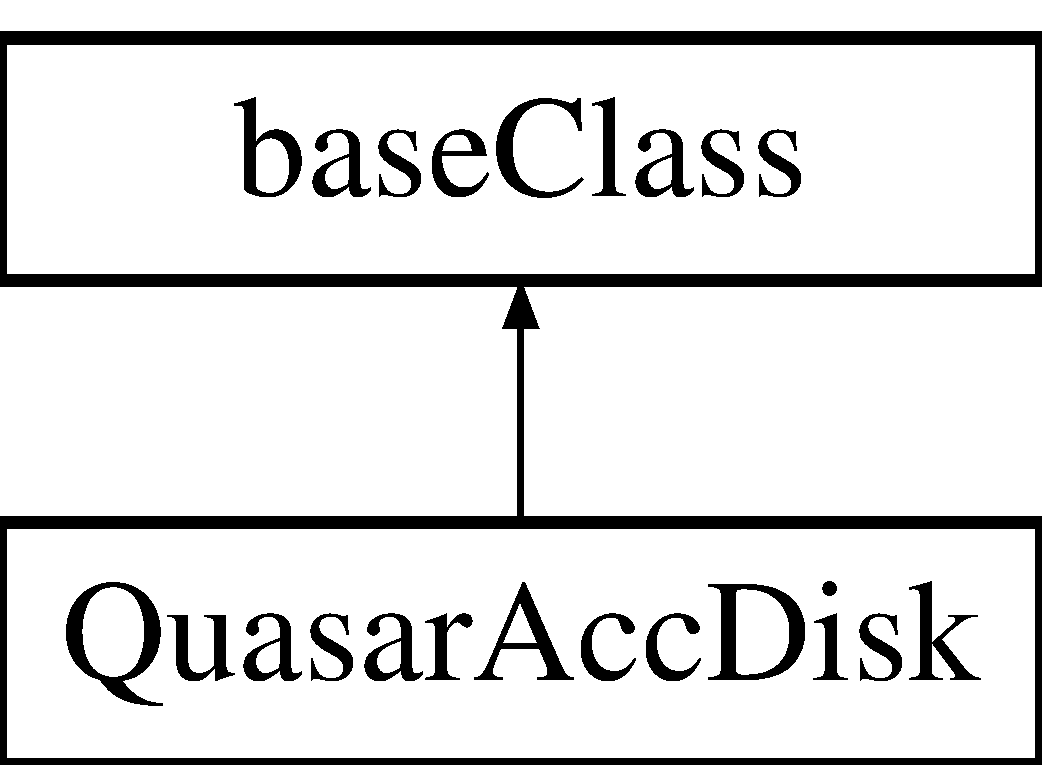
\includegraphics[height=2.000000cm]{classQuasarAccDisk}
\end{center}
\end{figure}


\subsection{Detailed Description}
Class used to process quasar radiation template and add it to calculated jet radiation; at the moment quasar radiation is not stricty calculated but a radius-\/loud quasar radiation template from Elvis et al. (1994) is used. Class has some basic methods to calculate standard multitemperature Shakura-\/\-Sunyayev disk radiation but it is not used currently as it need much, much detailed study and modelling of dusty torus, coronae etc \subsection*{Public Member Functions}
\begin{DoxyCompactItemize}
\item 
\hyperlink{classQuasarAccDisk_af3ebbefab21b01d1a4d86199fb2f643c}{Quasar\-Acc\-Disk} (scfgp $\ast$\-\_\-cfg, std\-::string \-\_\-id)
\item 
\hyperlink{classQuasarAccDisk_ab562cc81ade45ea51cf3ab27f7885d07}{$\sim$\-Quasar\-Acc\-Disk} ()
\item 
void \hyperlink{classQuasarAccDisk_aab9e9fbad17ba40931219473918896a7}{print\-Info} ()
\item 
double \hyperlink{classQuasarAccDisk_ac4abec686db321e73e0186ae8c6cd16c}{get\-Temperature} (double \-\_\-r)
\item 
double \hyperlink{classQuasarAccDisk_a8a29f029fd2e38784bce7dbe8f9533d2}{calculate\-Lv} (double v, int radius\-\_\-index)
\item 
void \hyperlink{classQuasarAccDisk_a60c8439e66b7a9933e35eeb6fe12dd89}{calculate\-Luminosity} ()
\item 
void \hyperlink{classQuasarAccDisk_ad565b960520076ca8e82d10286e05aef}{set\-Radius} ()
\item 
void \hyperlink{classQuasarAccDisk_a8f1f855a229a0247e3b4af731b9d7b29}{set\-Energetics} ()
\item 
int \hyperlink{classQuasarAccDisk_a8e81488ad8604d0b4b1ebb904a5830da}{read\-Template} ()
\item 
void \hyperlink{classQuasarAccDisk_a632f415a0df6afd015f27c8ae447129b}{scale\-Template} ()
\item 
int \hyperlink{classQuasarAccDisk_a64ce6d4ea6be61e97b9bc5c1a87398e5}{save\-Template} ()
\item 
void \hyperlink{classQuasarAccDisk_a88d65d7d654293daedabbb0ecbd81d72}{allocate\-Lv} ()
\item 
\hypertarget{classQuasarAccDisk_a5369e43384d98b527114e81412445b56}{void {\bfseries free\-Lv} ()}\label{classQuasarAccDisk_a5369e43384d98b527114e81412445b56}

\item 
\hypertarget{classQuasarAccDisk_ac9ad8e0fd51bfa2fa8fdd6140e4f1830}{void {\bfseries allocate\-Lv\-Template} ()}\label{classQuasarAccDisk_ac9ad8e0fd51bfa2fa8fdd6140e4f1830}

\item 
\hypertarget{classQuasarAccDisk_a43bf4ee038beb51661aede7e8bea452a}{void {\bfseries free\-Lv\-Template} ()}\label{classQuasarAccDisk_a43bf4ee038beb51661aede7e8bea452a}

\item 
\hypertarget{classQuasarAccDisk_a9bd872ab0f30ba940185a801174d0ee4}{void {\bfseries set\-\_\-v} (int i, double val)}\label{classQuasarAccDisk_a9bd872ab0f30ba940185a801174d0ee4}

\item 
\hypertarget{classQuasarAccDisk_a0fc9028abafdf012d4f0edb99f9624db}{void {\bfseries set\-\_\-\-Lv} (int i, double val)}\label{classQuasarAccDisk_a0fc9028abafdf012d4f0edb99f9624db}

\item 
\hypertarget{classQuasarAccDisk_a4384e3fbeae13417a9ad69b6fed5a609}{int {\bfseries get\-N} ()}\label{classQuasarAccDisk_a4384e3fbeae13417a9ad69b6fed5a609}

\item 
\hypertarget{classQuasarAccDisk_a7dfc8b822bc5f71a9d481a6467edc466}{gsl\-\_\-vector $\ast$ {\bfseries get\-\_\-v} ()}\label{classQuasarAccDisk_a7dfc8b822bc5f71a9d481a6467edc466}

\item 
\hypertarget{classQuasarAccDisk_adc29e040d3f5f4362379a71f584d8186}{gsl\-\_\-vector $\ast$ {\bfseries get\-\_\-\-Lv} ()}\label{classQuasarAccDisk_adc29e040d3f5f4362379a71f584d8186}

\item 
\hypertarget{classQuasarAccDisk_a7adca85d6b441a5f911ffd395a0ac179}{int {\bfseries get\-\_\-save\-\_\-\-Lr} ()}\label{classQuasarAccDisk_a7adca85d6b441a5f911ffd395a0ac179}

\end{DoxyCompactItemize}
\subsection*{Public Attributes}
\begin{DoxyCompactItemize}
\item 
gsl\-\_\-vector $\ast$ \hyperlink{classQuasarAccDisk_a9ec136403f3df7f3a2582968a28fdfcb}{v\-Template}
\item 
\hypertarget{classQuasarAccDisk_a85f88e9936d636004014fa3893de6abe}{gsl\-\_\-vector $\ast$ {\bfseries Lv\-Template}}\label{classQuasarAccDisk_a85f88e9936d636004014fa3893de6abe}

\item 
\hyperlink{classlogGeometry}{log\-Geometry} $\ast$ \hyperlink{classQuasarAccDisk_a470359d2a40c176d5eef36a7bf2fc5bf}{R}
\end{DoxyCompactItemize}


\subsection{Constructor \& Destructor Documentation}
\hypertarget{classQuasarAccDisk_af3ebbefab21b01d1a4d86199fb2f643c}{\index{Quasar\-Acc\-Disk@{Quasar\-Acc\-Disk}!Quasar\-Acc\-Disk@{Quasar\-Acc\-Disk}}
\index{Quasar\-Acc\-Disk@{Quasar\-Acc\-Disk}!QuasarAccDisk@{Quasar\-Acc\-Disk}}
\subsubsection[{Quasar\-Acc\-Disk}]{\setlength{\rightskip}{0pt plus 5cm}Quasar\-Acc\-Disk\-::\-Quasar\-Acc\-Disk (
\begin{DoxyParamCaption}
\item[{scfgp $\ast$}]{\-\_\-cfg, }
\item[{std\-::string}]{\-\_\-id}
\end{DoxyParamCaption}
)}}\label{classQuasarAccDisk_af3ebbefab21b01d1a4d86199fb2f643c}
constructor 
\begin{DoxyParams}{Parameters}
{\em scfgp} & \\
\hline
{\em id} & \\
\hline
\end{DoxyParams}

\begin{DoxyCode}
8                                                          : \hyperlink{classbaseClass}{baseClass}( \_cfg, NULL, \_id ) \{
9   \textcolor{comment}{/* requested parameters */}
10   \hyperlink{classbaseClass_a744f87a6ebe63da08256c022d42a4ca7}{cfg} -> request<double>(\textcolor{stringliteral}{"mBH"},1.0,&mBH);
11   \hyperlink{classbaseClass_a744f87a6ebe63da08256c022d42a4ca7}{cfg} -> request<double>(\textcolor{stringliteral}{"mDot"},1.0,&mDot);
12   \hyperlink{classbaseClass_a744f87a6ebe63da08256c022d42a4ca7}{cfg} -> request<double>(\textcolor{stringliteral}{"eDisk"},0.1,&eDisk);
13   \hyperlink{classbaseClass_a744f87a6ebe63da08256c022d42a4ca7}{cfg} -> request<int>(\textcolor{stringliteral}{"N"} + \hyperlink{classbaseClass_a4d5ff386a69bcbe21b5976f55b624df6}{id}, 200, &N );
14   \hyperlink{classbaseClass_a744f87a6ebe63da08256c022d42a4ca7}{cfg} -> request<double>(\textcolor{keywordtype}{id} + \textcolor{stringliteral}{"R1"}, 0.0, &R1 );
15   \hyperlink{classbaseClass_a744f87a6ebe63da08256c022d42a4ca7}{cfg} -> request<double>(\textcolor{keywordtype}{id} + \textcolor{stringliteral}{"R2"}, 0.0, &R2 );
16   \hyperlink{classbaseClass_a744f87a6ebe63da08256c022d42a4ca7}{cfg} -> request<std::string>(\textcolor{keywordtype}{id} + \textcolor{stringliteral}{"TemplateFilename"}, \textcolor{stringliteral}{"dat/elvisRL.dat"}, &templateFilename );
17 
18   \hyperlink{classbaseClass_a744f87a6ebe63da08256c022d42a4ca7}{cfg} -> request<int>(\textcolor{keywordtype}{id} + \textcolor{stringliteral}{"SaveLr"}, 0, &save\_Lr);
19 
20   \hyperlink{classbaseClass_a744f87a6ebe63da08256c022d42a4ca7}{cfg} -> updateRequests( );
21 
22   \hyperlink{classQuasarAccDisk_a8f1f855a229a0247e3b4af731b9d7b29}{setEnergetics}( );
23 
24   \textcolor{keywordflow}{if}( R1 == 0.0 || R2 == 0.0 ) \{ \hyperlink{classQuasarAccDisk_ad565b960520076ca8e82d10286e05aef}{setRadius}( ); \}
25 
26   vMin = 1.0e12;
27   vMax = 1.0e18;
28 
29   numLines = 0;
30 
31   \hyperlink{classQuasarAccDisk_a88d65d7d654293daedabbb0ecbd81d72}{allocateLv}( );
32 
33   \textcolor{keywordflow}{for}( \textcolor{keywordtype}{int} i=0;i<N;i++ ) \{ set\_v( i, vMin*pow( vMax/vMin,(\textcolor{keywordtype}{double})i/((\textcolor{keywordtype}{double})N-1)) ); \}
34   \hyperlink{classQuasarAccDisk_a470359d2a40c176d5eef36a7bf2fc5bf}{R} = \textcolor{keyword}{new} \hyperlink{classlogGeometry}{logGeometry}( R1, R2, 1000 );
35 \}
\end{DoxyCode}
\hypertarget{classQuasarAccDisk_ab562cc81ade45ea51cf3ab27f7885d07}{\index{Quasar\-Acc\-Disk@{Quasar\-Acc\-Disk}!$\sim$\-Quasar\-Acc\-Disk@{$\sim$\-Quasar\-Acc\-Disk}}
\index{$\sim$\-Quasar\-Acc\-Disk@{$\sim$\-Quasar\-Acc\-Disk}!QuasarAccDisk@{Quasar\-Acc\-Disk}}
\subsubsection[{$\sim$\-Quasar\-Acc\-Disk}]{\setlength{\rightskip}{0pt plus 5cm}Quasar\-Acc\-Disk\-::$\sim$\-Quasar\-Acc\-Disk (
\begin{DoxyParamCaption}
{}
\end{DoxyParamCaption}
)}}\label{classQuasarAccDisk_ab562cc81ade45ea51cf3ab27f7885d07}
destructor 
\begin{DoxyCode}
37                                \{
38   freeLv( );
39   freeLvTemplate( );
40 \}
\end{DoxyCode}


\subsection{Member Function Documentation}
\hypertarget{classQuasarAccDisk_a88d65d7d654293daedabbb0ecbd81d72}{\index{Quasar\-Acc\-Disk@{Quasar\-Acc\-Disk}!allocate\-Lv@{allocate\-Lv}}
\index{allocate\-Lv@{allocate\-Lv}!QuasarAccDisk@{Quasar\-Acc\-Disk}}
\subsubsection[{allocate\-Lv}]{\setlength{\rightskip}{0pt plus 5cm}void Quasar\-Acc\-Disk\-::allocate\-Lv (
\begin{DoxyParamCaption}
{}
\end{DoxyParamCaption}
)}}\label{classQuasarAccDisk_a88d65d7d654293daedabbb0ecbd81d72}
methods to allocate and free memory 
\begin{DoxyCode}
173                                 \{
174   v = gsl\_vector\_alloc( N );
175   Lv = gsl\_vector\_alloc( N );
176   bazinga::print\_GSLVector\_allocated\_memory( \textcolor{keywordtype}{id}, v );
177   bazinga::print\_GSLVector\_allocated\_memory( \textcolor{keywordtype}{id}, Lv );
178   gsl\_vector\_set\_zero( v );
179   gsl\_vector\_set\_zero( Lv ); \}
\end{DoxyCode}
\hypertarget{classQuasarAccDisk_a60c8439e66b7a9933e35eeb6fe12dd89}{\index{Quasar\-Acc\-Disk@{Quasar\-Acc\-Disk}!calculate\-Luminosity@{calculate\-Luminosity}}
\index{calculate\-Luminosity@{calculate\-Luminosity}!QuasarAccDisk@{Quasar\-Acc\-Disk}}
\subsubsection[{calculate\-Luminosity}]{\setlength{\rightskip}{0pt plus 5cm}void Quasar\-Acc\-Disk\-::calculate\-Luminosity (
\begin{DoxyParamCaption}
{}
\end{DoxyParamCaption}
)}}\label{classQuasarAccDisk_a60c8439e66b7a9933e35eeb6fe12dd89}
calculate a whole disk luminosity 
\begin{DoxyCode}
197                                          \{
198   bazinga::info(\textcolor{keywordtype}{id},\textcolor{stringliteral}{"Calculating luminosity."});
199   gsl\_vector* tempLv = gsl\_vector\_alloc( N );
200 
201   \textcolor{keywordflow}{for}( \textcolor{keywordtype}{int} i=0;i<\hyperlink{classQuasarAccDisk_a470359d2a40c176d5eef36a7bf2fc5bf}{R}->getMaxIndex();i++ ) \{
202     \hyperlink{classQuasarAccDisk_a470359d2a40c176d5eef36a7bf2fc5bf}{R} -> update( i );
203     gsl\_vector\_set\_zero( tempLv );
204 
205     \textcolor{keywordflow}{for}( \textcolor{keywordtype}{int} j=0;j<N;j++ ) \{
206       \textcolor{keywordflow}{if}( save\_Lr ) \{
207     gsl\_vector\_set( tempLv, j, \hyperlink{classQuasarAccDisk_a8a29f029fd2e38784bce7dbe8f9533d2}{calculateLv}( gsl\_vector\_get(v,j), i ) ); \}
208       gsl\_vector\_set( Lv, j, gsl\_vector\_get( Lv, j ) + \hyperlink{classQuasarAccDisk_a8a29f029fd2e38784bce7dbe8f9533d2}{calculateLv}( gsl\_vector\_get(v,j), i ) );
209     \}
210 
211     \textcolor{keywordflow}{if}( save\_Lr ) \{
212       std::string type = \textcolor{stringliteral}{"Lv\_"};
213       type += this->\hyperlink{classbaseClass_a756d5accf10ced9a34024048c95a51c9}{whoAmI}( );
214       bazinga::print\_info(\textcolor{keywordtype}{id},\textcolor{stringliteral}{"Saving QLuminosity."},\hyperlink{classQuasarAccDisk_a470359d2a40c176d5eef36a7bf2fc5bf}{R}->get( )/\hyperlink{classQuasarAccDisk_a470359d2a40c176d5eef36a7bf2fc5bf}{R}->getR0( ));
215       bazinga::save\_GSLVector( type, v, tempLv, \hyperlink{classQuasarAccDisk_a470359d2a40c176d5eef36a7bf2fc5bf}{R}->get( )/\hyperlink{classQuasarAccDisk_a470359d2a40c176d5eef36a7bf2fc5bf}{R}->getR0( ), \hyperlink{classbaseClass_a744f87a6ebe63da08256c022d42a4ca7}{cfg}->get<std::string>(\textcolor{stringliteral}{"output"})
       ); \}
216   \}
217 
218   gsl\_vector\_free( tempLv );
219   tempLv = NULL;
220 
221   std::string type = \textcolor{stringliteral}{"Lv\_"};
222   type += this->\hyperlink{classbaseClass_a756d5accf10ced9a34024048c95a51c9}{whoAmI}( );
223   bazinga::info(\textcolor{keywordtype}{id},\textcolor{stringliteral}{"Saving QLuminosity."});
224   bazinga::save\_GSLVector( type, v, Lv, \hyperlink{classbaseClass_a744f87a6ebe63da08256c022d42a4ca7}{cfg}->get<std::string>(\textcolor{stringliteral}{"output"}) );
225 
226   \textcolor{keywordtype}{double} integral = 0.0;
227   tempLv = gsl\_vector\_alloc( N );
228   gsl\_vector\_set\_zero( tempLv );
229   gsl\_vector\_memcpy( tempLv, Lv );
230   gsl\_vector\_mul( tempLv, v );
231   integral = loglogIntegrate( v, tempLv );
232   bazinga::print\_info( \textcolor{keywordtype}{id}, \textcolor{stringliteral}{"Acc Disk Lbol"}, integral );    
233 \}
\end{DoxyCode}
\hypertarget{classQuasarAccDisk_a8a29f029fd2e38784bce7dbe8f9533d2}{\index{Quasar\-Acc\-Disk@{Quasar\-Acc\-Disk}!calculate\-Lv@{calculate\-Lv}}
\index{calculate\-Lv@{calculate\-Lv}!QuasarAccDisk@{Quasar\-Acc\-Disk}}
\subsubsection[{calculate\-Lv}]{\setlength{\rightskip}{0pt plus 5cm}double Quasar\-Acc\-Disk\-::calculate\-Lv (
\begin{DoxyParamCaption}
\item[{double}]{v, }
\item[{int}]{radius\-\_\-index}
\end{DoxyParamCaption}
)}}\label{classQuasarAccDisk_a8a29f029fd2e38784bce7dbe8f9533d2}
calculate disk luminosity 
\begin{DoxyParams}{Parameters}
{\em frequency} & v \\
\hline
{\em radius\-\_\-index} & \\
\hline
\end{DoxyParams}

\begin{DoxyCode}
235                                                    \{
236   \textcolor{keywordtype}{double} val = ( 16.0*pow(M\_PI,2)*PLANCK\_H*cos(0.0)*pow(v,3) )/( pow(LIGHT\_SPEED,2) );
237   \textcolor{keywordflow}{return} val*( \hyperlink{classQuasarAccDisk_a470359d2a40c176d5eef36a7bf2fc5bf}{R}->get(i)*\hyperlink{classQuasarAccDisk_a470359d2a40c176d5eef36a7bf2fc5bf}{R}->getDr(i) )/( exp( (PLANCK\_H*v)/(K\_BOLTZMAN*
      \hyperlink{classQuasarAccDisk_ac4abec686db321e73e0186ae8c6cd16c}{getTemperature}(\hyperlink{classQuasarAccDisk_a470359d2a40c176d5eef36a7bf2fc5bf}{R}->get(i)) ) ) - 1.0 );
238 \}
\end{DoxyCode}
\hypertarget{classQuasarAccDisk_ac4abec686db321e73e0186ae8c6cd16c}{\index{Quasar\-Acc\-Disk@{Quasar\-Acc\-Disk}!get\-Temperature@{get\-Temperature}}
\index{get\-Temperature@{get\-Temperature}!QuasarAccDisk@{Quasar\-Acc\-Disk}}
\subsubsection[{get\-Temperature}]{\setlength{\rightskip}{0pt plus 5cm}double Quasar\-Acc\-Disk\-::get\-Temperature (
\begin{DoxyParamCaption}
\item[{double}]{\-\_\-r}
\end{DoxyParamCaption}
)}}\label{classQuasarAccDisk_ac4abec686db321e73e0186ae8c6cd16c}
get B\-B temperature at distance r (S\-S disk) 
\begin{DoxyParams}{Parameters}
{\em radius} & r \\
\hline
\end{DoxyParams}

\begin{DoxyCode}
168                                                 \{
169   \textcolor{keywordtype}{double} Risco = 6.0*Rg;
170   \textcolor{keywordflow}{return} pow( ( 3.0*G\_CONST*1.3e56*pow(mBH,2)*MSUN*mDot )*( 1.0-sqrt(Risco/\_r) )/( 8.0*M\_PI*pow(\_r, 3)*
      SIGMA\_SB*pow(LIGHT\_SPEED,2) ), 0.25 );
171 \}
\end{DoxyCode}
\hypertarget{classQuasarAccDisk_aab9e9fbad17ba40931219473918896a7}{\index{Quasar\-Acc\-Disk@{Quasar\-Acc\-Disk}!print\-Info@{print\-Info}}
\index{print\-Info@{print\-Info}!QuasarAccDisk@{Quasar\-Acc\-Disk}}
\subsubsection[{print\-Info}]{\setlength{\rightskip}{0pt plus 5cm}void Quasar\-Acc\-Disk\-::print\-Info (
\begin{DoxyParamCaption}
{}
\end{DoxyParamCaption}
)\hspace{0.3cm}{\ttfamily [virtual]}}}\label{classQuasarAccDisk_aab9e9fbad17ba40931219473918896a7}
print basic information about myself (virtual) 

Reimplemented from \hyperlink{classbaseClass_a67f911cca483b620b908c69dfa4f3ad7}{base\-Class}.


\begin{DoxyCode}
154                                \{
155   bazinga::info( \textcolor{keywordtype}{id}, \textcolor{stringliteral}{"Info"} );
156   bazinga::print\_info( \textcolor{keywordtype}{id}, \textcolor{stringliteral}{"N"}, N );
157   bazinga::print\_info( \textcolor{keywordtype}{id}, \textcolor{stringliteral}{"Gravitational radius"}, Rg, \textcolor{stringliteral}{"cm"} );
158   bazinga::print\_info( \textcolor{keywordtype}{id}, \textcolor{stringliteral}{"R1"}, R1, \textcolor{stringliteral}{"cm"} );
159   bazinga::print\_info( \textcolor{keywordtype}{id}, \textcolor{stringliteral}{"R2"}, R2, \textcolor{stringliteral}{"cm"} );
160   bazinga::print\_info( \textcolor{keywordtype}{id}, \textcolor{stringliteral}{"Save luminosity"}, save\_Lr );
161   bazinga::print\_info(\textcolor{keywordtype}{id},\textcolor{stringliteral}{"BH mass"},mBH);
162   bazinga::print\_info(\textcolor{keywordtype}{id},\textcolor{stringliteral}{"eta disk"},eDisk);
163   bazinga::print\_info(\textcolor{keywordtype}{id},\textcolor{stringliteral}{"m dot"},mDot);
164   bazinga::print\_info(\textcolor{keywordtype}{id},\textcolor{stringliteral}{"Eddington luminosity"},Ledd,\textcolor{stringliteral}{"erg/s"});
165   bazinga::print\_info( \textcolor{keywordtype}{id}, \textcolor{stringliteral}{"Accretion disk luminosity"}, Ldisk, \textcolor{stringliteral}{"erg/s"});
166 \}
\end{DoxyCode}
\hypertarget{classQuasarAccDisk_a8e81488ad8604d0b4b1ebb904a5830da}{\index{Quasar\-Acc\-Disk@{Quasar\-Acc\-Disk}!read\-Template@{read\-Template}}
\index{read\-Template@{read\-Template}!QuasarAccDisk@{Quasar\-Acc\-Disk}}
\subsubsection[{read\-Template}]{\setlength{\rightskip}{0pt plus 5cm}int Quasar\-Acc\-Disk\-::read\-Template (
\begin{DoxyParamCaption}
{}
\end{DoxyParamCaption}
)}}\label{classQuasarAccDisk_a8e81488ad8604d0b4b1ebb904a5830da}
read quasar radiation template \begin{DoxyReturn}{Returns}
1 if success; 0 otherwise 
\end{DoxyReturn}

\begin{DoxyCode}
115                                 \{
116   std::ifstream input( templateFilename.c\_str() );
117   bazinga::print\_info( \textcolor{keywordtype}{id}, \textcolor{stringliteral}{"Reading quasar template data from file "},templateFilename.c\_str());
118      \textcolor{keywordflow}{if}( input == NULL )
119     \{
120       bazinga::error(\textcolor{keywordtype}{id},\textcolor{stringliteral}{"Opening file:"},templateFilename);
121       \textcolor{keywordflow}{return} 1;
122     \}
123       \textcolor{keywordflow}{else}
124     \{
125       \textcolor{comment}{// check how many lines there are}
126       std::string unused;
127       \textcolor{keywordflow}{while} ( std::getline(input, unused) )
128         ++numLines;
129       
130       bazinga::print\_info(\textcolor{keywordtype}{id},\textcolor{stringliteral}{"Found"},numLines,\textcolor{stringliteral}{"lines"});
131       
132       \textcolor{comment}{// allocate space for vectors}
133       allocateLvTemplate( );
134 
135       \textcolor{comment}{// read data from template}
136       input.clear();
137       input.seekg(0, std::ios::beg);
138       \textcolor{keywordtype}{double} x, y;
139       \textcolor{keywordtype}{int} i = 0; \textcolor{comment}{// gsl counter}
140       \textcolor{keywordflow}{while}( std::getline(input, unused) ) \{
141       std::istringstream ss(unused);
142       std::istream\_iterator<std::string> begin(ss), end;
143       
144       \textcolor{comment}{//putting all the tokens in the vector}
145       std::vector<std::string> arrayTokens(begin, end); 
146       
147       gsl\_vector\_set( \hyperlink{classQuasarAccDisk_a9ec136403f3df7f3a2582968a28fdfcb}{vTemplate}, i, atof( arrayTokens[0].c\_str() ) );
148       gsl\_vector\_set( LvTemplate, i, atof( arrayTokens[1].c\_str() ) );           
149       ++i; \}
150       \textcolor{keywordflow}{return} 0;
151     \}
152 \}
\end{DoxyCode}
\hypertarget{classQuasarAccDisk_a64ce6d4ea6be61e97b9bc5c1a87398e5}{\index{Quasar\-Acc\-Disk@{Quasar\-Acc\-Disk}!save\-Template@{save\-Template}}
\index{save\-Template@{save\-Template}!QuasarAccDisk@{Quasar\-Acc\-Disk}}
\subsubsection[{save\-Template}]{\setlength{\rightskip}{0pt plus 5cm}int Quasar\-Acc\-Disk\-::save\-Template (
\begin{DoxyParamCaption}
{}
\end{DoxyParamCaption}
)}}\label{classQuasarAccDisk_a64ce6d4ea6be61e97b9bc5c1a87398e5}
save scaled quasar radiation template 
\begin{DoxyCode}
101                                  \{
102   std::string type = \textcolor{stringliteral}{"LvTemplate\_"}+this->\hyperlink{classbaseClass_a756d5accf10ced9a34024048c95a51c9}{whoAmI}( );
103   bazinga::info(this->\hyperlink{classbaseClass_a756d5accf10ced9a34024048c95a51c9}{whoAmI}( ),\textcolor{stringliteral}{"Saving luminosity."});
104 
105   gsl\_vector* LvTemplateTemp = gsl\_vector\_alloc( numLines );
106   gsl\_vector\_set\_zero( LvTemplateTemp );
107   gsl\_vector\_memcpy( LvTemplateTemp, LvTemplate );
108   gsl\_vector\_div( LvTemplateTemp, \hyperlink{classQuasarAccDisk_a9ec136403f3df7f3a2582968a28fdfcb}{vTemplate} );
109     
110   bazinga::save\_GSLVector( type, this->\hyperlink{classQuasarAccDisk_a9ec136403f3df7f3a2582968a28fdfcb}{vTemplate}, LvTemplateTemp, \hyperlink{classbaseClass_a744f87a6ebe63da08256c022d42a4ca7}{cfg}->get<std::string>(\textcolor{stringliteral}{"output
      "}) );
111   gsl\_vector\_free( LvTemplateTemp );
112   LvTemplateTemp = NULL;
113  \}
\end{DoxyCode}
\hypertarget{classQuasarAccDisk_a632f415a0df6afd015f27c8ae447129b}{\index{Quasar\-Acc\-Disk@{Quasar\-Acc\-Disk}!scale\-Template@{scale\-Template}}
\index{scale\-Template@{scale\-Template}!QuasarAccDisk@{Quasar\-Acc\-Disk}}
\subsubsection[{scale\-Template}]{\setlength{\rightskip}{0pt plus 5cm}void Quasar\-Acc\-Disk\-::scale\-Template (
\begin{DoxyParamCaption}
{}
\end{DoxyParamCaption}
)}}\label{classQuasarAccDisk_a632f415a0df6afd015f27c8ae447129b}
scale quasar radiation template to match set accretion disk efficiency 
\begin{DoxyCode}
49                                    \{
50   \textcolor{keywordtype}{double} integral = loglogIntegrate( \hyperlink{classQuasarAccDisk_a9ec136403f3df7f3a2582968a28fdfcb}{vTemplate}, LvTemplate );
51   \textcolor{keywordtype}{double} correctionFactor = Ldisk/integral;
52   bazinga::print\_info( \textcolor{keywordtype}{id}, \textcolor{stringliteral}{"Template correction factor"}, correctionFactor );
53   gsl\_vector\_scale( LvTemplate, correctionFactor );
54   integral = loglogIntegrate( \hyperlink{classQuasarAccDisk_a9ec136403f3df7f3a2582968a28fdfcb}{vTemplate}, LvTemplate );
55   bazinga::print\_info( \textcolor{keywordtype}{id}, \textcolor{stringliteral}{"Template Lbol after correction"}, integral );
56   
57   \textcolor{comment}{// Find peak in IR, Optical and X-ray}
58   \textcolor{keywordtype}{double} IRmin = 1.0e10;
59   \textcolor{keywordtype}{double} IRmax = 2.0e14;
60   \textcolor{keywordtype}{double} OPTmin = IRmax;
61   \textcolor{keywordtype}{double} OPTmax = 7.0e16;
62   \textcolor{keywordtype}{double} Xmin = OPTmax;
63   \textcolor{keywordtype}{double} Xmax = 1.0e20;
64 
65   \textcolor{keywordtype}{double} vIRpeak = 0.0;
66   \textcolor{keywordtype}{double} vOPTpeak = 0.0;
67   \textcolor{keywordtype}{double} vXpeak = 0.0;
68 
69   \textcolor{keywordtype}{double} vLvIRpeak = 0.0;
70   \textcolor{keywordtype}{double} vLvOPTpeak = 0.0;
71   \textcolor{keywordtype}{double} vLvXpeak = 0.0;
72   
73   \textcolor{keywordflow}{for}( \textcolor{keywordtype}{int} i=0; i<\hyperlink{classQuasarAccDisk_a9ec136403f3df7f3a2582968a28fdfcb}{vTemplate}->size-1; ++i ) \{
74     \textcolor{keywordflow}{if}( gsl\_vector\_get( \hyperlink{classQuasarAccDisk_a9ec136403f3df7f3a2582968a28fdfcb}{vTemplate}, i ) >= IRmin && gsl\_vector\_get( 
      \hyperlink{classQuasarAccDisk_a9ec136403f3df7f3a2582968a28fdfcb}{vTemplate}, i ) <= IRmax )
75       \textcolor{keywordflow}{if}( gsl\_vector\_get( LvTemplate, i ) > vLvIRpeak ) \{
76     vLvIRpeak = gsl\_vector\_get( LvTemplate, i );
77     vIRpeak = gsl\_vector\_get( \hyperlink{classQuasarAccDisk_a9ec136403f3df7f3a2582968a28fdfcb}{vTemplate}, i ); \}
78   \}
79   bazinga::print\_info( \textcolor{keywordtype}{id}, \textcolor{stringliteral}{"IR template v peak"}, vIRpeak );
80   bazinga::print\_info( \textcolor{keywordtype}{id}, \textcolor{stringliteral}{"IR template vLv peak"}, vLvIRpeak );
81 
82   \textcolor{keywordflow}{for}( \textcolor{keywordtype}{int} i=0; i<\hyperlink{classQuasarAccDisk_a9ec136403f3df7f3a2582968a28fdfcb}{vTemplate}->size-1; ++i ) \{
83     \textcolor{keywordflow}{if}( gsl\_vector\_get( \hyperlink{classQuasarAccDisk_a9ec136403f3df7f3a2582968a28fdfcb}{vTemplate}, i ) >= OPTmin && gsl\_vector\_get( 
      \hyperlink{classQuasarAccDisk_a9ec136403f3df7f3a2582968a28fdfcb}{vTemplate}, i ) <= OPTmax )
84       \textcolor{keywordflow}{if}( gsl\_vector\_get( LvTemplate, i ) > vLvOPTpeak ) \{
85     vLvOPTpeak = gsl\_vector\_get( LvTemplate, i );
86     vOPTpeak = gsl\_vector\_get( \hyperlink{classQuasarAccDisk_a9ec136403f3df7f3a2582968a28fdfcb}{vTemplate}, i ); \}
87   \}
88   bazinga::print\_info( \textcolor{keywordtype}{id}, \textcolor{stringliteral}{"OPT template v peak"}, vOPTpeak );
89   bazinga::print\_info( \textcolor{keywordtype}{id}, \textcolor{stringliteral}{"OPT template vLv peak"}, vLvOPTpeak );
90 
91   \textcolor{keywordflow}{for}( \textcolor{keywordtype}{int} i=0; i<\hyperlink{classQuasarAccDisk_a9ec136403f3df7f3a2582968a28fdfcb}{vTemplate}->size-1; ++i ) \{
92     \textcolor{keywordflow}{if}( gsl\_vector\_get( \hyperlink{classQuasarAccDisk_a9ec136403f3df7f3a2582968a28fdfcb}{vTemplate}, i ) >= Xmin && gsl\_vector\_get( 
      \hyperlink{classQuasarAccDisk_a9ec136403f3df7f3a2582968a28fdfcb}{vTemplate}, i ) <= Xmax )
93       \textcolor{keywordflow}{if}( gsl\_vector\_get( LvTemplate, i ) > vLvXpeak ) \{
94     vLvXpeak = gsl\_vector\_get( LvTemplate, i );
95     vXpeak = gsl\_vector\_get( \hyperlink{classQuasarAccDisk_a9ec136403f3df7f3a2582968a28fdfcb}{vTemplate}, i ); \}
96   \}
97   bazinga::print\_info( \textcolor{keywordtype}{id}, \textcolor{stringliteral}{"X template v peak"}, vXpeak );
98   bazinga::print\_info( \textcolor{keywordtype}{id}, \textcolor{stringliteral}{"X template vLv peak"}, vLvXpeak );
99 \}
\end{DoxyCode}
\hypertarget{classQuasarAccDisk_a8f1f855a229a0247e3b4af731b9d7b29}{\index{Quasar\-Acc\-Disk@{Quasar\-Acc\-Disk}!set\-Energetics@{set\-Energetics}}
\index{set\-Energetics@{set\-Energetics}!QuasarAccDisk@{Quasar\-Acc\-Disk}}
\subsubsection[{set\-Energetics}]{\setlength{\rightskip}{0pt plus 5cm}void Quasar\-Acc\-Disk\-::set\-Energetics (
\begin{DoxyParamCaption}
{}
\end{DoxyParamCaption}
)}}\label{classQuasarAccDisk_a8f1f855a229a0247e3b4af731b9d7b29}
set energetics for further calculations 
\begin{DoxyCode}
247                                    \{
248    Ledd = 1.3e47*mBH;
249    Ldisk = eDisk*mDot*Ledd; \}
\end{DoxyCode}
\hypertarget{classQuasarAccDisk_ad565b960520076ca8e82d10286e05aef}{\index{Quasar\-Acc\-Disk@{Quasar\-Acc\-Disk}!set\-Radius@{set\-Radius}}
\index{set\-Radius@{set\-Radius}!QuasarAccDisk@{Quasar\-Acc\-Disk}}
\subsubsection[{set\-Radius}]{\setlength{\rightskip}{0pt plus 5cm}void Quasar\-Acc\-Disk\-::set\-Radius (
\begin{DoxyParamCaption}
{}
\end{DoxyParamCaption}
)}}\label{classQuasarAccDisk_ad565b960520076ca8e82d10286e05aef}
set accretion disk radial boundaries 
\begin{DoxyCode}
240                                \{
241   \textcolor{comment}{/* gravitational radius */}
242   Rg = (2.0*G\_CONST*mBH*1.0e9*MSUN)/pow(LIGHT\_SPEED,2);
243   R1 = 6.0*Rg;
244   \textcolor{keywordtype}{double} R\_sub = 1.6e-5*sqrt( Ldisk );
245   R2 = R\_sub; \}
\end{DoxyCode}


\subsection{Member Data Documentation}
\hypertarget{classQuasarAccDisk_a470359d2a40c176d5eef36a7bf2fc5bf}{\index{Quasar\-Acc\-Disk@{Quasar\-Acc\-Disk}!R@{R}}
\index{R@{R}!QuasarAccDisk@{Quasar\-Acc\-Disk}}
\subsubsection[{R}]{\setlength{\rightskip}{0pt plus 5cm}{\bf log\-Geometry}$\ast$ Quasar\-Acc\-Disk\-::\-R}}\label{classQuasarAccDisk_a470359d2a40c176d5eef36a7bf2fc5bf}
\hyperlink{classlogGeometry}{log\-Geometry} to store log-\/spaced data for loglog-\/interpolation \hypertarget{classQuasarAccDisk_a9ec136403f3df7f3a2582968a28fdfcb}{\index{Quasar\-Acc\-Disk@{Quasar\-Acc\-Disk}!v\-Template@{v\-Template}}
\index{v\-Template@{v\-Template}!QuasarAccDisk@{Quasar\-Acc\-Disk}}
\subsubsection[{v\-Template}]{\setlength{\rightskip}{0pt plus 5cm}gsl\-\_\-vector$\ast$ Quasar\-Acc\-Disk\-::v\-Template}}\label{classQuasarAccDisk_a9ec136403f3df7f3a2582968a28fdfcb}
vectors to store data 

The documentation for this class was generated from the following files\-:\begin{DoxyCompactItemize}
\item 
/home/mjaniak/\-Soft/blazar++/include/\hyperlink{QuasarAccDisk_8hpp}{Quasar\-Acc\-Disk.\-hpp}\item 
/home/mjaniak/\-Soft/blazar++/src/\hyperlink{QuasarAccDisk_8cpp}{Quasar\-Acc\-Disk.\-cpp}\end{DoxyCompactItemize}

\hypertarget{classselfSynCompton}{\section{self\-Syn\-Compton Class Reference}
\label{classselfSynCompton}\index{self\-Syn\-Compton@{self\-Syn\-Compton}}
}


{\ttfamily \#include $<$self\-Syn\-Compton.\-hpp$>$}

Inheritance diagram for self\-Syn\-Compton\-:\begin{figure}[H]
\begin{center}
\leavevmode
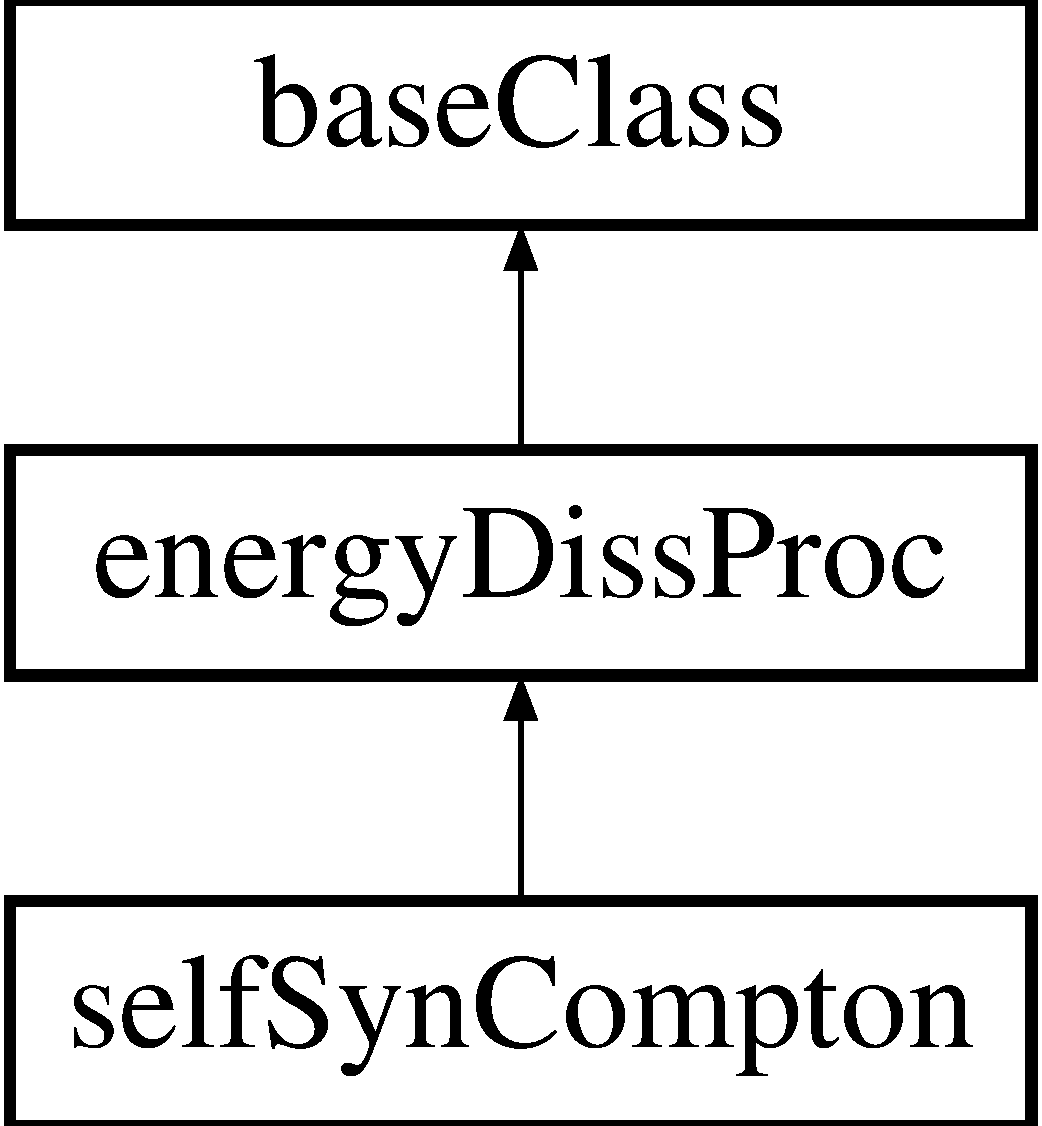
\includegraphics[height=3.000000cm]{classselfSynCompton}
\end{center}
\end{figure}


\subsection{Detailed Description}
Class provides S\-S\-C electron energy losses and S\-S\-C luminosity calculation \subsection*{Public Member Functions}
\begin{DoxyCompactItemize}
\item 
\hyperlink{classselfSynCompton_a577dca084342cabf74de2765f0b187d0}{self\-Syn\-Compton} (scfgp $\ast$\-\_\-cfg, \hyperlink{classjetGeometry}{jet\-Geometry} $\ast$\-\_\-r, \hyperlink{classelectrons}{electrons} $\ast$\-\_\-ele, \hyperlink{classmagneticField}{magnetic\-Field} $\ast$\-\_\-\-B, std\-::string \-\_\-id)
\item 
\hyperlink{classselfSynCompton_adc3ac6dc66cc436b48d0a36ab26871fd}{$\sim$self\-Syn\-Compton} ()
\item 
void \hyperlink{classselfSynCompton_a46f692985a0fd74c14a018cc43f25c0b}{print\-Info} ()
\item 
double \hyperlink{classselfSynCompton_a51bad50f11e56a623b80e4436ef1b629}{dotg} (double g)
\item 
void \hyperlink{classselfSynCompton_af254f0dcd2abfe1d218c85d917992e24}{update} ()
\item 
double \hyperlink{classselfSynCompton_a39e8b6e7b4094f39f9436cd94a15775e}{calculate\-Lpv} (double v)
\item 
void \hyperlink{classselfSynCompton_ae34a13d5ddf894d3e1ede229ffb4176a}{set\-Lpv} ()
\end{DoxyCompactItemize}
\subsection*{Public Attributes}
\begin{DoxyCompactItemize}
\item 
\hyperlink{classmagneticField}{magnetic\-Field} $\ast$ \hyperlink{classselfSynCompton_a7f24c41ccf47e77fefab4c946e9397f6}{B}
\item 
\hyperlink{classenergyDissProc}{energy\-Diss\-Proc} $\ast$ \hyperlink{classselfSynCompton_a98b1421fe0ab8028d180d16d48ccbcc8}{syn}
\end{DoxyCompactItemize}


\subsection{Constructor \& Destructor Documentation}
\hypertarget{classselfSynCompton_a577dca084342cabf74de2765f0b187d0}{\index{self\-Syn\-Compton@{self\-Syn\-Compton}!self\-Syn\-Compton@{self\-Syn\-Compton}}
\index{self\-Syn\-Compton@{self\-Syn\-Compton}!selfSynCompton@{self\-Syn\-Compton}}
\subsubsection[{self\-Syn\-Compton}]{\setlength{\rightskip}{0pt plus 5cm}self\-Syn\-Compton\-::self\-Syn\-Compton (
\begin{DoxyParamCaption}
\item[{scfgp $\ast$}]{\-\_\-cfg, }
\item[{{\bf jet\-Geometry} $\ast$}]{\-\_\-r, }
\item[{{\bf electrons} $\ast$}]{\-\_\-ele, }
\item[{{\bf magnetic\-Field} $\ast$}]{\-\_\-\-B, }
\item[{std\-::string}]{\-\_\-id}
\end{DoxyParamCaption}
)}}\label{classselfSynCompton_a577dca084342cabf74de2765f0b187d0}
constructor 
\begin{DoxyParams}{Parameters}
{\em \-\_\-cfg} & -\/ scfgp class object \\
\hline
{\em \-\_\-r} & -\/ \hyperlink{classjetGeometry}{jet\-Geometry} class object \\
\hline
{\em \-\_\-ele} & -\/ electrons class object \\
\hline
{\em \-\_\-\-B} & -\/ \hyperlink{classmagneticField}{magnetic\-Field} class object \\
\hline
{\em \-\_\-id} & \\
\hline
\end{DoxyParams}

\begin{DoxyCode}
9                                                                                                            
           : \hyperlink{classenergyDissProc_a0cf0b423089016fbe8a697378c519590}{energyDissProc}( \_cfg, \_r, \_ele, \_id  ), \hyperlink{classselfSynCompton_a7f24c41ccf47e77fefab4c946e9397f6}{B}(\_B) \{
10   \textcolor{comment}{/* requested parameters */}
11   \hyperlink{classbaseClass_a744f87a6ebe63da08256c022d42a4ca7}{cfg} -> request<int>(\textcolor{stringliteral}{"N"}+\hyperlink{classbaseClass_a4d5ff386a69bcbe21b5976f55b624df6}{id},200,&\hyperlink{classbaseClass_a2b4d07d2b46197d495de0477f4bb22f8}{N});
12   \hyperlink{classbaseClass_a744f87a6ebe63da08256c022d42a4ca7}{cfg} -> request<int>(\textcolor{stringliteral}{"KN"},0,&KN);
13   
14   \hyperlink{classbaseClass_a744f87a6ebe63da08256c022d42a4ca7}{cfg} -> updateRequests( );
15 
16   \hyperlink{classenergyDissProc_aafedd3c012010a8e8aa34247660fea3b}{vpMin} = 1.0;
17   \textcolor{comment}{/* here we set vpMAX to a maximum value specified by maximal value of magnetic field at R0 */}
18   vpMax = 100.0*A43*DSQR(\hyperlink{classenergyDissProc_a0dbf0777938131e938c1fdad5df38a7f}{ele}->getGammaMax( ))*DSQR(\hyperlink{classenergyDissProc_a0dbf0777938131e938c1fdad5df38a7f}{ele}->getGammaMax( ))*( 
      \hyperlink{classselfSynCompton_a7f24c41ccf47e77fefab4c946e9397f6}{B}->\hyperlink{classmagneticField_a3b573d12649137290d521539b903da8d}{getMaxB}( )/B\_CR )*mec2h;
19 
20   allocateUpe( );
21   allocateUpeR( );
22   allocateLpv( );
23   allocateLvPoint( );
24   allocateLvPointAvg( );
25 
26   \textcolor{keywordflow}{for}( \textcolor{keywordtype}{int} i=0;i<\hyperlink{classbaseClass_a2b4d07d2b46197d495de0477f4bb22f8}{N};i++ ) \{ set\_vp( i, \hyperlink{classenergyDissProc_aafedd3c012010a8e8aa34247660fea3b}{vpMin}*pow( vpMax/\hyperlink{classenergyDissProc_aafedd3c012010a8e8aa34247660fea3b}{vpMin},(\textcolor{keywordtype}{double})i/((\textcolor{keywordtype}{double})N-1)) ); \}
27  \}
\end{DoxyCode}
\hypertarget{classselfSynCompton_adc3ac6dc66cc436b48d0a36ab26871fd}{\index{self\-Syn\-Compton@{self\-Syn\-Compton}!$\sim$self\-Syn\-Compton@{$\sim$self\-Syn\-Compton}}
\index{$\sim$self\-Syn\-Compton@{$\sim$self\-Syn\-Compton}!selfSynCompton@{self\-Syn\-Compton}}
\subsubsection[{$\sim$self\-Syn\-Compton}]{\setlength{\rightskip}{0pt plus 5cm}self\-Syn\-Compton\-::$\sim$self\-Syn\-Compton (
\begin{DoxyParamCaption}
{}
\end{DoxyParamCaption}
)}}\label{classselfSynCompton_adc3ac6dc66cc436b48d0a36ab26871fd}
destructor 
\begin{DoxyCode}
29                                  \{
30   freeLpv( );
31   freeLvPoint( );
32   freeLvPointAvg( );
33   freeUpe( ); \}
\end{DoxyCode}


\subsection{Member Function Documentation}
\hypertarget{classselfSynCompton_a39e8b6e7b4094f39f9436cd94a15775e}{\index{self\-Syn\-Compton@{self\-Syn\-Compton}!calculate\-Lpv@{calculate\-Lpv}}
\index{calculate\-Lpv@{calculate\-Lpv}!selfSynCompton@{self\-Syn\-Compton}}
\subsubsection[{calculate\-Lpv}]{\setlength{\rightskip}{0pt plus 5cm}double self\-Syn\-Compton\-::calculate\-Lpv (
\begin{DoxyParamCaption}
\item[{double}]{v}
\end{DoxyParamCaption}
)\hspace{0.3cm}{\ttfamily [virtual]}}}\label{classselfSynCompton_a39e8b6e7b4094f39f9436cd94a15775e}
calculate intrinsic luminosity 
\begin{DoxyParams}{Parameters}
{\em v} & -\/ frequency (jet co-\/moving frame) \\
\hline
\end{DoxyParams}
\begin{DoxyReturn}{Returns}
L'\-\_\-v 
\end{DoxyReturn}


Reimplemented from \hyperlink{classenergyDissProc_aed17a9ce8a970cbd1e250c59947407ac}{energy\-Diss\-Proc}.


\begin{DoxyCode}
59                                               \{
60   \textcolor{keywordtype}{double} dg,de,j;
61   \textcolor{keywordtype}{double} Int1;
62   \textcolor{keywordtype}{double} e;
63   Int1 = 0.0;
64   j = 0.0;
65 
66   e = PLANCK\_H*v/(ELECTRON\_MASS*LIGHT\_SPEED*LIGHT\_SPEED);
67   
68   dg = \hyperlink{classenergyDissProc_a0dbf0777938131e938c1fdad5df38a7f}{ele}->\hyperlink{classelectrons_a4e3d4179ce211bd732580b49914874e6}{getdLogGamma}( );
69   de = \hyperlink{classselfSynCompton_a98b1421fe0ab8028d180d16d48ccbcc8}{syn}->\hyperlink{classenergyDissProc_a5ef88d9ecacade52bbd277695230d237}{getdLogE}( );
70 
71   \textcolor{keywordflow}{for}( \textcolor{keywordtype}{int} i=0; i<\hyperlink{classselfSynCompton_a98b1421fe0ab8028d180d16d48ccbcc8}{syn}->\hyperlink{classbaseClass_a6ba5c4ce24742db73f45064337cf6963}{getN}( );i++ ) \{
72     Int1 = 0.0;
73     \textcolor{comment}{/* integration over electron energy (gamma) */}
74     \textcolor{keywordflow}{for}( \textcolor{keywordtype}{int} k=0;k<\hyperlink{classenergyDissProc_a0dbf0777938131e938c1fdad5df38a7f}{ele}->\hyperlink{classbaseClass_a6ba5c4ce24742db73f45064337cf6963}{getN}( );k++ ) \{ 
75       Int1  += bazinga::IntCor( k, \hyperlink{classenergyDissProc_a0dbf0777938131e938c1fdad5df38a7f}{ele}->\hyperlink{classbaseClass_a6ba5c4ce24742db73f45064337cf6963}{getN}( ) )*inverseCompton::fiso( 
      \hyperlink{classenergyDissProc_a0dbf0777938131e938c1fdad5df38a7f}{ele}->\hyperlink{classelectrons_afb0d9365f13787f44d23fb489732fc90}{getGamma}(k), \hyperlink{classselfSynCompton_a98b1421fe0ab8028d180d16d48ccbcc8}{syn}->get\_ep(i),e )*\hyperlink{classenergyDissProc_a0dbf0777938131e938c1fdad5df38a7f}{ele}->\hyperlink{classelectrons_a24fbbed0acac968ce6b2ef2c5043dee4}{getNgamma}(k)/
      \hyperlink{classenergyDissProc_a0dbf0777938131e938c1fdad5df38a7f}{ele}->\hyperlink{classelectrons_afb0d9365f13787f44d23fb489732fc90}{getGamma}(k); \}
76     
77       \textcolor{comment}{/* integration over seed photon energy */}
78     j += bazinga::IntCor( i, \hyperlink{classselfSynCompton_a98b1421fe0ab8028d180d16d48ccbcc8}{syn}->\hyperlink{classbaseClass_a6ba5c4ce24742db73f45064337cf6963}{getN}( ) )*\hyperlink{classselfSynCompton_a98b1421fe0ab8028d180d16d48ccbcc8}{syn}->get\_upe(i)/\hyperlink{classselfSynCompton_a98b1421fe0ab8028d180d16d48ccbcc8}{syn}->get\_ep(i)*Int1*dg; \}
79 
80   j *= constC1*e*de;
81   \textcolor{keywordflow}{return} j; \}
\end{DoxyCode}
\hypertarget{classselfSynCompton_a51bad50f11e56a623b80e4436ef1b629}{\index{self\-Syn\-Compton@{self\-Syn\-Compton}!dotg@{dotg}}
\index{dotg@{dotg}!selfSynCompton@{self\-Syn\-Compton}}
\subsubsection[{dotg}]{\setlength{\rightskip}{0pt plus 5cm}double self\-Syn\-Compton\-::dotg (
\begin{DoxyParamCaption}
\item[{double}]{g}
\end{DoxyParamCaption}
)\hspace{0.3cm}{\ttfamily [virtual]}}}\label{classselfSynCompton_a51bad50f11e56a623b80e4436ef1b629}
get d gamma \textbackslash{} d t for particular process 
\begin{DoxyParams}{Parameters}
{\em g} & -\/ electron Lorentz factor \\
\hline
\end{DoxyParams}
\begin{DoxyReturn}{Returns}
d gamma \textbackslash{} d t 
\end{DoxyReturn}


Reimplemented from \hyperlink{classenergyDissProc_a8074e0db5d859a8815e7136c2fc41b46}{energy\-Diss\-Proc}.


\begin{DoxyCode}
42                                       \{
43   \textcolor{keywordtype}{double} b,sum, val = 0.0;
44 
45   \textcolor{keywordflow}{for}( \textcolor{keywordtype}{int} i=0;i<\hyperlink{classselfSynCompton_a98b1421fe0ab8028d180d16d48ccbcc8}{syn}->\hyperlink{classbaseClass_a6ba5c4ce24742db73f45064337cf6963}{getN}( );i++ ) \{
46     b = 4.0*\hyperlink{classselfSynCompton_a98b1421fe0ab8028d180d16d48ccbcc8}{syn}->get\_ep(i)*g;
47     \textcolor{keywordflow}{if}( b > 1.0 ) \{ \hyperlink{classenergyDissProc_a69ea4be814273e47e69e31e593c3a250}{set\_KN\_info}( g ); \}
48     sum += bazinga::IntCor( i, \hyperlink{classselfSynCompton_a98b1421fe0ab8028d180d16d48ccbcc8}{syn}->\hyperlink{classbaseClass_a6ba5c4ce24742db73f45064337cf6963}{getN}( ) )*\hyperlink{classselfSynCompton_a98b1421fe0ab8028d180d16d48ccbcc8}{syn}->get\_ep(i)*\hyperlink{classselfSynCompton_a98b1421fe0ab8028d180d16d48ccbcc8}{syn}->get\_upe(i)*
      inverseCompton::fKN( b, KN ); \}
49   
50   val = \hyperlink{classselfSynCompton_a98b1421fe0ab8028d180d16d48ccbcc8}{syn}->\hyperlink{classenergyDissProc_a5ef88d9ecacade52bbd277695230d237}{getdLogE}( )*sum;
51   
52   set\_upe\_r( val );  
53   \textcolor{keywordflow}{return}( val ); \}
\end{DoxyCode}
\hypertarget{classselfSynCompton_a46f692985a0fd74c14a018cc43f25c0b}{\index{self\-Syn\-Compton@{self\-Syn\-Compton}!print\-Info@{print\-Info}}
\index{print\-Info@{print\-Info}!selfSynCompton@{self\-Syn\-Compton}}
\subsubsection[{print\-Info}]{\setlength{\rightskip}{0pt plus 5cm}void self\-Syn\-Compton\-::print\-Info (
\begin{DoxyParamCaption}
{}
\end{DoxyParamCaption}
)\hspace{0.3cm}{\ttfamily [virtual]}}}\label{classselfSynCompton_a46f692985a0fd74c14a018cc43f25c0b}
print basic information about myself (virtual) 

Reimplemented from \hyperlink{classenergyDissProc_ad1fbde0f7635a19a81412b9766916eb9}{energy\-Diss\-Proc}.


\begin{DoxyCode}
35                                 \{
36   bazinga::info(\textcolor{keywordtype}{id},\textcolor{stringliteral}{"Info"});
37   bazinga::print\_info(\textcolor{keywordtype}{id},\textcolor{stringliteral}{"N"},\hyperlink{classbaseClass_a2b4d07d2b46197d495de0477f4bb22f8}{N});
38   bazinga::print\_info(\textcolor{keywordtype}{id},\textcolor{stringliteral}{"KN"},KN); \}
\end{DoxyCode}
\hypertarget{classselfSynCompton_ae34a13d5ddf894d3e1ede229ffb4176a}{\index{self\-Syn\-Compton@{self\-Syn\-Compton}!set\-Lpv@{set\-Lpv}}
\index{set\-Lpv@{set\-Lpv}!selfSynCompton@{self\-Syn\-Compton}}
\subsubsection[{set\-Lpv}]{\setlength{\rightskip}{0pt plus 5cm}void self\-Syn\-Compton\-::set\-Lpv (
\begin{DoxyParamCaption}
{}
\end{DoxyParamCaption}
)\hspace{0.3cm}{\ttfamily [virtual]}}}\label{classselfSynCompton_ae34a13d5ddf894d3e1ede229ffb4176a}
set intrinsic luminosities 

Reimplemented from \hyperlink{classenergyDissProc_a93a39df53f30801f9f057cd55c05485d}{energy\-Diss\-Proc}.


\begin{DoxyCode}
55                              \{
56   \textcolor{keywordflow}{for}( \textcolor{keywordtype}{int} i=0;i<\hyperlink{classbaseClass_a2b4d07d2b46197d495de0477f4bb22f8}{N};i++ ) \{ set\_Lpv( i, \hyperlink{classselfSynCompton_a39e8b6e7b4094f39f9436cd94a15775e}{calculateLpv}( get\_vp(i) ) ); \} 
57 \}
\end{DoxyCode}
\hypertarget{classselfSynCompton_af254f0dcd2abfe1d218c85d917992e24}{\index{self\-Syn\-Compton@{self\-Syn\-Compton}!update@{update}}
\index{update@{update}!selfSynCompton@{self\-Syn\-Compton}}
\subsubsection[{update}]{\setlength{\rightskip}{0pt plus 5cm}void self\-Syn\-Compton\-::update (
\begin{DoxyParamCaption}
{}
\end{DoxyParamCaption}
)\hspace{0.3cm}{\ttfamily [virtual]}}}\label{classselfSynCompton_af254f0dcd2abfe1d218c85d917992e24}
update all process internal parameters to current radius 

Reimplemented from \hyperlink{classenergyDissProc_a6033524ea3d0fe38056bd74622f6c4ad}{energy\-Diss\-Proc}.


\begin{DoxyCode}
40 \{ \hyperlink{classenergyDissProc_a7b51925f603e271657cab66afe822591}{flag\_upe\_r} = \textcolor{keyword}{false}; \}
\end{DoxyCode}


\subsection{Member Data Documentation}
\hypertarget{classselfSynCompton_a7f24c41ccf47e77fefab4c946e9397f6}{\index{self\-Syn\-Compton@{self\-Syn\-Compton}!B@{B}}
\index{B@{B}!selfSynCompton@{self\-Syn\-Compton}}
\subsubsection[{B}]{\setlength{\rightskip}{0pt plus 5cm}{\bf magnetic\-Field}$\ast$ self\-Syn\-Compton\-::\-B}}\label{classselfSynCompton_a7f24c41ccf47e77fefab4c946e9397f6}
magenetic field B' \hypertarget{classselfSynCompton_a98b1421fe0ab8028d180d16d48ccbcc8}{\index{self\-Syn\-Compton@{self\-Syn\-Compton}!syn@{syn}}
\index{syn@{syn}!selfSynCompton@{self\-Syn\-Compton}}
\subsubsection[{syn}]{\setlength{\rightskip}{0pt plus 5cm}{\bf energy\-Diss\-Proc}$\ast$ self\-Syn\-Compton\-::syn}}\label{classselfSynCompton_a98b1421fe0ab8028d180d16d48ccbcc8}
synchrotron process pointer 

The documentation for this class was generated from the following files\-:\begin{DoxyCompactItemize}
\item 
/home/mjaniak/\-Soft/blazar++/include/\hyperlink{selfSynCompton_8hpp}{self\-Syn\-Compton.\-hpp}\item 
/home/mjaniak/\-Soft/blazar++/src/\hyperlink{selfSynCompton_8cpp}{self\-Syn\-Compton.\-cpp}\end{DoxyCompactItemize}

\hypertarget{classstruct}{\section{struct Class Reference}
\label{classstruct}\index{struct@{struct}}
}


\subsection{Detailed Description}
used to calculate break in electron energy 

The documentation for this class was generated from the following file\-:\begin{DoxyCompactItemize}
\item 
/home/mjaniak/\-Soft/blazar++/include/\hyperlink{electrons_8hpp}{electrons.\-hpp}\end{DoxyCompactItemize}

\hypertarget{classsynchrotron}{\section{synchrotron Class Reference}
\label{classsynchrotron}\index{synchrotron@{synchrotron}}
}


{\ttfamily \#include $<$synchrotron.\-hpp$>$}

Inheritance diagram for synchrotron\-:\begin{figure}[H]
\begin{center}
\leavevmode
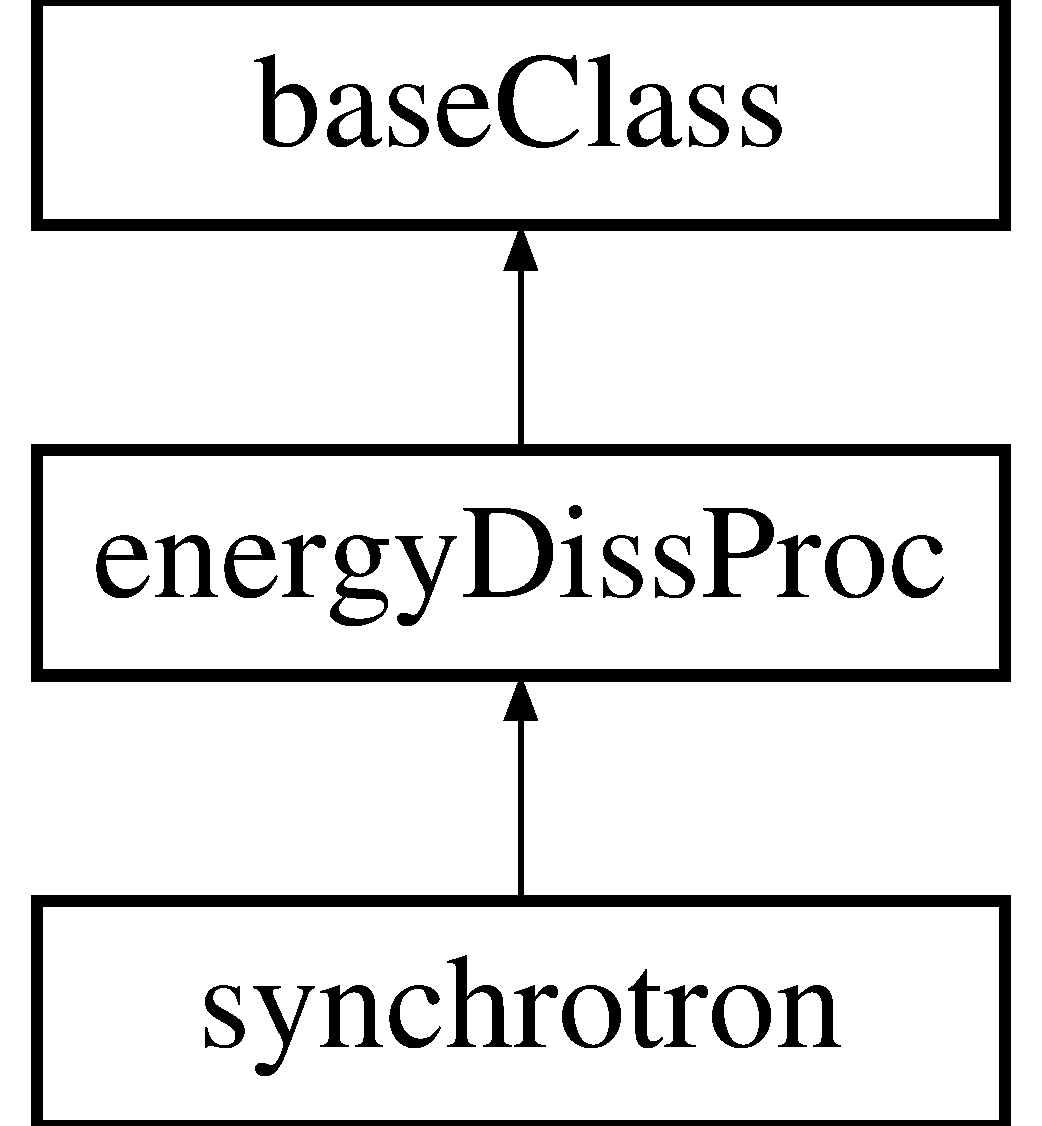
\includegraphics[height=3.000000cm]{classsynchrotron}
\end{center}
\end{figure}


\subsection{Detailed Description}
Class provides synchrotron electron energy losses and synchrotron luminosity calculation \subsection*{Public Member Functions}
\begin{DoxyCompactItemize}
\item 
\hyperlink{classsynchrotron_ab02aaf0264ad332a77524487993e122b}{synchrotron} (scfgp $\ast$\-\_\-cfg, \hyperlink{classjetGeometry}{jet\-Geometry} $\ast$\-\_\-r, \hyperlink{classelectrons}{electrons} $\ast$\-\_\-ele, \hyperlink{classmagneticField}{magnetic\-Field} $\ast$\-\_\-\-B, std\-::string \-\_\-id)
\item 
\hyperlink{classsynchrotron_a5a4aed3b6187a30e25343753ea5e4fa6}{$\sim$synchrotron} ()
\item 
void \hyperlink{classsynchrotron_a6a8610b523a6e3c656372537ad28b756}{print\-Info} ()
\item 
double \hyperlink{classsynchrotron_a0587f0a1da199ec87019a96589fcb58c}{iterate} ()
\item 
double \hyperlink{classsynchrotron_a577e2fa11ba90bf288099e88f02c756f}{dotg} (double g)
\item 
void \hyperlink{classsynchrotron_a52ec26284de15395bd203037024b7ae4}{update} ()
\item 
void \hyperlink{classsynchrotron_adf30d0e7cbba05a39a16b60957d02321}{set\-Lpv} ()
\item 
double \hyperlink{classsynchrotron_ab12acf6ee2bdc60011e2739ba42cd32a}{calculate\-Lpv} (double v)
\end{DoxyCompactItemize}
\subsection*{Additional Inherited Members}


\subsection{Constructor \& Destructor Documentation}
\hypertarget{classsynchrotron_ab02aaf0264ad332a77524487993e122b}{\index{synchrotron@{synchrotron}!synchrotron@{synchrotron}}
\index{synchrotron@{synchrotron}!synchrotron@{synchrotron}}
\subsubsection[{synchrotron}]{\setlength{\rightskip}{0pt plus 5cm}synchrotron\-::synchrotron (
\begin{DoxyParamCaption}
\item[{scfgp $\ast$}]{\-\_\-cfg, }
\item[{{\bf jet\-Geometry} $\ast$}]{\-\_\-r, }
\item[{{\bf electrons} $\ast$}]{\-\_\-ele, }
\item[{{\bf magnetic\-Field} $\ast$}]{\-\_\-\-B, }
\item[{std\-::string}]{\-\_\-id}
\end{DoxyParamCaption}
)}}\label{classsynchrotron_ab02aaf0264ad332a77524487993e122b}
constructor 
\begin{DoxyParams}{Parameters}
{\em \-\_\-cfg} & -\/ scfgp class object \\
\hline
{\em \-\_\-r} & -\/ \hyperlink{classjetGeometry}{jet\-Geometry} class object \\
\hline
{\em \-\_\-ele} & -\/ electrons class object \\
\hline
{\em \-\_\-\-B} & -\/ magnetic field class object \\
\hline
{\em \-\_\-id} & \\
\hline
\end{DoxyParams}

\begin{DoxyCode}
9                                                                                                           :
       \hyperlink{classenergyDissProc_a0cf0b423089016fbe8a697378c519590}{energyDissProc}( \_cfg, \_r, \_ele, \_id ), B(\_B) \{
10   \textcolor{comment}{/* requested parameters */}
11   \hyperlink{classbaseClass_a744f87a6ebe63da08256c022d42a4ca7}{cfg} -> request<int>(\textcolor{stringliteral}{"N"}+\hyperlink{classbaseClass_a4d5ff386a69bcbe21b5976f55b624df6}{id},200,&\hyperlink{classbaseClass_a2b4d07d2b46197d495de0477f4bb22f8}{N});
12   \hyperlink{classbaseClass_a744f87a6ebe63da08256c022d42a4ca7}{cfg} -> request<std::string>(\textcolor{stringliteral}{"lumModel"},\textcolor{stringliteral}{"blob"},&lumModel);
13   \hyperlink{classbaseClass_a744f87a6ebe63da08256c022d42a4ca7}{cfg} -> request<double>(\textcolor{stringliteral}{"thetaJ"},0.1,&thetaJ);
14   \hyperlink{classbaseClass_a744f87a6ebe63da08256c022d42a4ca7}{cfg} -> request<double>(\textcolor{stringliteral}{"Gamma"},10.0,&Gamma);
15   \hyperlink{classbaseClass_a744f87a6ebe63da08256c022d42a4ca7}{cfg} -> request<int>(\textcolor{stringliteral}{"SABS"},1,&SABS);
16   \hyperlink{classbaseClass_a744f87a6ebe63da08256c022d42a4ca7}{cfg} -> request<int>(\textcolor{keywordtype}{id}+\textcolor{stringliteral}{"LuminosityConstU"},0,&\hyperlink{classenergyDissProc_a2cc4e4eae15982f977a0dfa5458d80f4}{luminosityConstU});  
17   \hyperlink{classbaseClass_a744f87a6ebe63da08256c022d42a4ca7}{cfg} -> request<int>(\textcolor{keywordtype}{id}+\textcolor{stringliteral}{"LuminosityConstNu"},0,&\hyperlink{classenergyDissProc_a0a23854c1c830dfb9ac33d116fce5b7d}{luminosityConstNu});  
18   \hyperlink{classbaseClass_a744f87a6ebe63da08256c022d42a4ca7}{cfg} -> request<int>(\textcolor{stringliteral}{"setSSCBlob"},0,&setSSCBlob);  
19 
20   \hyperlink{classbaseClass_a744f87a6ebe63da08256c022d42a4ca7}{cfg} -> updateRequests( );
21 
22   \hyperlink{classenergyDissProc_aafedd3c012010a8e8aa34247660fea3b}{vpMin} = 1.0;
23   \textcolor{comment}{/* here we set vpMAX to a maximum value specified by maximal value of magnetic field at R0 */}
24   vpMax = 100.0*A43*DSQR(\hyperlink{classenergyDissProc_a0dbf0777938131e938c1fdad5df38a7f}{ele}->getGammaMax( ))*( B->\hyperlink{classmagneticField_a3b573d12649137290d521539b903da8d}{getMaxB}( )/B\_CR )*mec2h;
25   \hyperlink{classenergyDissProc_a57aee74ef8fc4cb9220127a9c345174a}{epMin} = PLANCK\_H/mec2;
26   epMax = vpMax/mec2h;
27   
28   allocateUpe( );
29   allocateUpeR( );
30   allocateLpv( );
31   allocateLvPoint( );
32   allocateLvPointAvg( );
33 
34   \textcolor{keywordflow}{for}( \textcolor{keywordtype}{int} i=0;i<\hyperlink{classbaseClass_a2b4d07d2b46197d495de0477f4bb22f8}{N};i++ ) \{
35     set\_ep( i, epMax*pow( epMax/epMin,(\textcolor{keywordtype}{double})i/(\textcolor{keywordtype}{double})(N-1)) );
36     set\_vp( i, \hyperlink{classenergyDissProc_aafedd3c012010a8e8aa34247660fea3b}{vpMin}*pow( vpMax/\hyperlink{classenergyDissProc_aafedd3c012010a8e8aa34247660fea3b}{vpMin},(\textcolor{keywordtype}{double})i/((\textcolor{keywordtype}{double})N-1)) ); \}
37 
38   \hyperlink{classenergyDissProc_a270fdc20de5c26f9cc499f28dd32fb7b}{dLogE} = log(get\_ep(1)/get\_ep(0)); \}
\end{DoxyCode}
\hypertarget{classsynchrotron_a5a4aed3b6187a30e25343753ea5e4fa6}{\index{synchrotron@{synchrotron}!$\sim$synchrotron@{$\sim$synchrotron}}
\index{$\sim$synchrotron@{$\sim$synchrotron}!synchrotron@{synchrotron}}
\subsubsection[{$\sim$synchrotron}]{\setlength{\rightskip}{0pt plus 5cm}synchrotron\-::$\sim$synchrotron (
\begin{DoxyParamCaption}
{}
\end{DoxyParamCaption}
)}}\label{classsynchrotron_a5a4aed3b6187a30e25343753ea5e4fa6}
destructor 
\begin{DoxyCode}
40                            \{
41   freeLpv( );
42   freeLvPoint( );
43   freeLvPointAvg( );
44   freeUpe( ); \}
\end{DoxyCode}


\subsection{Member Function Documentation}
\hypertarget{classsynchrotron_ab12acf6ee2bdc60011e2739ba42cd32a}{\index{synchrotron@{synchrotron}!calculate\-Lpv@{calculate\-Lpv}}
\index{calculate\-Lpv@{calculate\-Lpv}!synchrotron@{synchrotron}}
\subsubsection[{calculate\-Lpv}]{\setlength{\rightskip}{0pt plus 5cm}double synchrotron\-::calculate\-Lpv (
\begin{DoxyParamCaption}
\item[{double}]{v}
\end{DoxyParamCaption}
)\hspace{0.3cm}{\ttfamily [virtual]}}}\label{classsynchrotron_ab12acf6ee2bdc60011e2739ba42cd32a}
calculate intrinsic luminosity 
\begin{DoxyParams}{Parameters}
{\em v} & -\/ frequency (jet co-\/moving frame) \\
\hline
\end{DoxyParams}
\begin{DoxyReturn}{Returns}
L'\-\_\-v 
\end{DoxyReturn}


Reimplemented from \hyperlink{classenergyDissProc_aed17a9ce8a970cbd1e250c59947407ac}{energy\-Diss\-Proc}.


\begin{DoxyCode}
91                                            \{
92   \textcolor{keywordtype}{double} a,jS,sigmaS,corr;
93   \textcolor{keywordtype}{double} vB,h,t,L,tau;
94   
95   vB = ELECTRON\_CHARGE*B->\hyperlink{classmagneticField_ac345cd6d5a111f0b96db08dadf65ff76}{getB}( )/(2.0*M\_PI*ELECTRON\_MASS*LIGHT\_SPEED);
96   h = \hyperlink{classenergyDissProc_a0dbf0777938131e938c1fdad5df38a7f}{ele}->\hyperlink{classelectrons_a4e3d4179ce211bd732580b49914874e6}{getdLogGamma}( );
97   L = tau = 0.0e0;
98 
99   \textcolor{keywordflow}{for}( \textcolor{keywordtype}{int} i=0;i<\hyperlink{classenergyDissProc_a0dbf0777938131e938c1fdad5df38a7f}{ele}->\hyperlink{classbaseClass_a6ba5c4ce24742db73f45064337cf6963}{getN}( );i++) \{
100       t = v/(3.0*DSQR( \hyperlink{classenergyDissProc_a0dbf0777938131e938c1fdad5df38a7f}{ele}->\hyperlink{classelectrons_afb0d9365f13787f44d23fb489732fc90}{getGamma}(i))*vB );
101       FS(t,&jS,&sigmaS);
102       tau += bazinga::IntCor( i, \hyperlink{classenergyDissProc_a0dbf0777938131e938c1fdad5df38a7f}{ele}->\hyperlink{classbaseClass_a6ba5c4ce24742db73f45064337cf6963}{getN}( ) )*sigmaS*\hyperlink{classenergyDissProc_a0dbf0777938131e938c1fdad5df38a7f}{ele}->\hyperlink{classelectrons_a24fbbed0acac968ce6b2ef2c5043dee4}{getNgamma}(i)/pow(
      \hyperlink{classenergyDissProc_a0dbf0777938131e938c1fdad5df38a7f}{ele}->\hyperlink{classelectrons_afb0d9365f13787f44d23fb489732fc90}{getGamma}(i),4);
103       L += bazinga::IntCor( i, \hyperlink{classenergyDissProc_a0dbf0777938131e938c1fdad5df38a7f}{ele}->\hyperlink{classbaseClass_a6ba5c4ce24742db73f45064337cf6963}{getN}( ) )*\hyperlink{classenergyDissProc_a0dbf0777938131e938c1fdad5df38a7f}{ele}->\hyperlink{classelectrons_afb0d9365f13787f44d23fb489732fc90}{getGamma}(i)*
      \hyperlink{classenergyDissProc_a0dbf0777938131e938c1fdad5df38a7f}{ele}->\hyperlink{classelectrons_a24fbbed0acac968ce6b2ef2c5043dee4}{getNgamma}(i)*jS; \}
104 
105   
106   \textcolor{keywordflow}{if}( SABS && (\hyperlink{classbaseClass_a482bb9b1d94f3eb3f31026d14e9a2bb6}{r}->get( )>=\hyperlink{classbaseClass_a482bb9b1d94f3eb3f31026d14e9a2bb6}{r}->getR0( )) ) \{
107       \textcolor{comment}{/* since in a there is r-r0 then first luminosity wont have absorption; original blazar code had
       different naming: }
108 \textcolor{comment}{     all quantities calculated at r were tagged as r+rd - we do not follow this approach thus r>*
      (model->R0) and not }
109 \textcolor{comment}{     r>=R0 (it gives errors) */}
110       \textcolor{comment}{/* I cheat; I set DR to be dr for r=R0; is it a bad approximation? I dunno */}
111       \textcolor{keywordtype}{double} DR = 0;
112       \textcolor{keywordflow}{if}( \hyperlink{classbaseClass_a482bb9b1d94f3eb3f31026d14e9a2bb6}{r}->get() == \hyperlink{classbaseClass_a482bb9b1d94f3eb3f31026d14e9a2bb6}{r}->getR0( ) ) \{ DR = \hyperlink{classbaseClass_a482bb9b1d94f3eb3f31026d14e9a2bb6}{r}->getDr(); \}
113       \textcolor{keywordflow}{else} \{ DR = \hyperlink{classbaseClass_a482bb9b1d94f3eb3f31026d14e9a2bb6}{r}->get( )-(\hyperlink{classbaseClass_a482bb9b1d94f3eb3f31026d14e9a2bb6}{r}->getR0( )); \}
114 
115       a = 2.0*DR/(\hyperlink{classbaseClass_a208facecf3a4480b47bebfce91413a39}{beta}(Gamma)*Gamma);
116       tau *= h*3.0/(4.0*M\_PI*a*a)*2.0*sqrt(3.0)*M\_PI/15.0*ELECTRON\_CHARGE/B->
      \hyperlink{classmagneticField_ac345cd6d5a111f0b96db08dadf65ff76}{getB}( );
117       corr = (tau>1.0e-5) ? (1.0-exp(-tau))/tau : (1.0-0.5*tau+1.0/6.0*tau*tau-1.0/24.0*pow(tau,3)+1.0/120.
      0*pow(tau,4)-1.0/720.0*pow(tau,5));
118   \} \textcolor{keywordflow}{else} \{ corr = 1.0e0; \}
119   
120   \textcolor{keywordflow}{if}( \hyperlink{classenergyDissProc_a2cc4e4eae15982f977a0dfa5458d80f4}{luminosityConstU} || \hyperlink{classenergyDissProc_a0a23854c1c830dfb9ac33d116fce5b7d}{luminosityConstNu} ) \{   L *= h*3.0*sqrt(3.0)*
      SIGMA\_T*LIGHT\_SPEED*B->\hyperlink{classmagneticField_ad1184833ba01cf9ef3fdf4bbd5b6f7f9}{get\_uB}( \hyperlink{classenergyDissProc_af1c1d91f8ef5f49f2f5831776052b651}{injRm} )/(M\_PI*vB)*corr; \}
121   \textcolor{keywordflow}{else} \{   L *= h*3.0*sqrt(3.0)*SIGMA\_T*LIGHT\_SPEED*B->\hyperlink{classmagneticField_ad1184833ba01cf9ef3fdf4bbd5b6f7f9}{get\_uB}( )/(M\_PI*vB)*corr; \}
122   
123   \textcolor{keywordflow}{return} L; \}
\end{DoxyCode}
\hypertarget{classsynchrotron_a577e2fa11ba90bf288099e88f02c756f}{\index{synchrotron@{synchrotron}!dotg@{dotg}}
\index{dotg@{dotg}!synchrotron@{synchrotron}}
\subsubsection[{dotg}]{\setlength{\rightskip}{0pt plus 5cm}double synchrotron\-::dotg (
\begin{DoxyParamCaption}
\item[{double}]{g}
\end{DoxyParamCaption}
)\hspace{0.3cm}{\ttfamily [virtual]}}}\label{classsynchrotron_a577e2fa11ba90bf288099e88f02c756f}
get d gamma \textbackslash{} d t for particular process 
\begin{DoxyParams}{Parameters}
{\em g} & -\/ electron Lorentz factor \\
\hline
\end{DoxyParams}
\begin{DoxyReturn}{Returns}
d gamma \textbackslash{} d t 
\end{DoxyReturn}


Reimplemented from \hyperlink{classenergyDissProc_a8074e0db5d859a8815e7136c2fc41b46}{energy\-Diss\-Proc}.


\begin{DoxyCode}
58 \{ \textcolor{keywordflow}{return} B->\hyperlink{classmagneticField_ad1184833ba01cf9ef3fdf4bbd5b6f7f9}{get\_uB}( ); \}
\end{DoxyCode}
\hypertarget{classsynchrotron_a0587f0a1da199ec87019a96589fcb58c}{\index{synchrotron@{synchrotron}!iterate@{iterate}}
\index{iterate@{iterate}!synchrotron@{synchrotron}}
\subsubsection[{iterate}]{\setlength{\rightskip}{0pt plus 5cm}double synchrotron\-::iterate (
\begin{DoxyParamCaption}
{}
\end{DoxyParamCaption}
)}}\label{classsynchrotron_a0587f0a1da199ec87019a96589fcb58c}
iterate synchrotron and S\-S\-C calculation to achieve steady state and balance between synchrotron and S\-S\-C luminosities 
\begin{DoxyCode}
125                              \{
126   \textcolor{keywordtype}{double} sumN = 0.0;
127   \textcolor{keywordtype}{double} err = 0.0;
128   gsl\_vector* temp\_upe = gsl\_vector\_alloc( \hyperlink{classbaseClass_a2b4d07d2b46197d495de0477f4bb22f8}{N} );
129   
130   \textcolor{comment}{/* copy current upe to temp\_upe */}
131   \textcolor{keywordflow}{for}( \textcolor{keywordtype}{int} i=0;i<\hyperlink{classbaseClass_a2b4d07d2b46197d495de0477f4bb22f8}{N};i++ ) \{ gsl\_vector\_set( temp\_upe, i, get\_upe( i ) ); \}
132 
133   \textcolor{comment}{/* calculate synchrotron energy densities and luminosities with new Ngamma*/}
134   \hyperlink{classsynchrotron_a52ec26284de15395bd203037024b7ae4}{update}( );
135       
136   \textcolor{keywordflow}{for}( \textcolor{keywordtype}{int} i=0;i<\hyperlink{classbaseClass_a2b4d07d2b46197d495de0477f4bb22f8}{N};i++ ) \{
137       sumN += get\_upe( i );
138       err += fabs( get\_upe( i ) - gsl\_vector\_get( temp\_upe, i ) ); \}
139   err /= sumN;
140   gsl\_vector\_free( temp\_upe );
141   temp\_upe = NULL;
142 
143   \textcolor{keywordflow}{return} err; \}
\end{DoxyCode}
\hypertarget{classsynchrotron_a6a8610b523a6e3c656372537ad28b756}{\index{synchrotron@{synchrotron}!print\-Info@{print\-Info}}
\index{print\-Info@{print\-Info}!synchrotron@{synchrotron}}
\subsubsection[{print\-Info}]{\setlength{\rightskip}{0pt plus 5cm}void synchrotron\-::print\-Info (
\begin{DoxyParamCaption}
{}
\end{DoxyParamCaption}
)\hspace{0.3cm}{\ttfamily [virtual]}}}\label{classsynchrotron_a6a8610b523a6e3c656372537ad28b756}
print basic information about myself (virtual) 

Reimplemented from \hyperlink{classenergyDissProc_ad1fbde0f7635a19a81412b9766916eb9}{energy\-Diss\-Proc}.


\begin{DoxyCode}
46                              \{
47   bazinga::info(\textcolor{keywordtype}{id},\textcolor{stringliteral}{"Info"});
48   bazinga::print\_info(\textcolor{keywordtype}{id},\textcolor{stringliteral}{"N"},\hyperlink{classbaseClass_a2b4d07d2b46197d495de0477f4bb22f8}{N});
49   bazinga::print\_info(\textcolor{keywordtype}{id},\textcolor{stringliteral}{"SABS"},SABS);
50   \textcolor{keywordflow}{if}( setSSCBlob ) \{ 
51     bazinga::print\_info(\textcolor{keywordtype}{id},\textcolor{stringliteral}{"setSSCBlob"},setSSCBlob); \}
52 
53   \textcolor{keywordflow}{if}( \hyperlink{classenergyDissProc_a2cc4e4eae15982f977a0dfa5458d80f4}{luminosityConstU} || \hyperlink{classenergyDissProc_a0a23854c1c830dfb9ac33d116fce5b7d}{luminosityConstNu} ) \{ 
54     bazinga::warning(\textcolor{keywordtype}{id},\textcolor{stringliteral}{"Using constant u' to calculate luminosity."});
55     bazinga::warning(\textcolor{keywordtype}{id},\textcolor{stringliteral}{"Using constant v' to calculate luminosity."}); \}
56 \}
\end{DoxyCode}
\hypertarget{classsynchrotron_adf30d0e7cbba05a39a16b60957d02321}{\index{synchrotron@{synchrotron}!set\-Lpv@{set\-Lpv}}
\index{set\-Lpv@{set\-Lpv}!synchrotron@{synchrotron}}
\subsubsection[{set\-Lpv}]{\setlength{\rightskip}{0pt plus 5cm}void synchrotron\-::set\-Lpv (
\begin{DoxyParamCaption}
{}
\end{DoxyParamCaption}
)\hspace{0.3cm}{\ttfamily [virtual]}}}\label{classsynchrotron_adf30d0e7cbba05a39a16b60957d02321}
set intrinsic luminosities 

Reimplemented from \hyperlink{classenergyDissProc_a93a39df53f30801f9f057cd55c05485d}{energy\-Diss\-Proc}.


\begin{DoxyCode}
74                           \{
75   \textcolor{keywordflow}{for}( \textcolor{keywordtype}{int} i=0;i<\hyperlink{classbaseClass_a2b4d07d2b46197d495de0477f4bb22f8}{N};i++ ) \{
76     set\_vp( i, \hyperlink{classenergyDissProc_aafedd3c012010a8e8aa34247660fea3b}{vpMin}*pow( vpMax/\hyperlink{classenergyDissProc_aafedd3c012010a8e8aa34247660fea3b}{vpMin},(\textcolor{keywordtype}{double})i/((\textcolor{keywordtype}{double})N-1)) );
77     set\_Lpv( i, \hyperlink{classsynchrotron_ab12acf6ee2bdc60011e2739ba42cd32a}{calculateLpv}( get\_vp(i) ) ); \}
78 \}
\end{DoxyCode}
\hypertarget{classsynchrotron_a52ec26284de15395bd203037024b7ae4}{\index{synchrotron@{synchrotron}!update@{update}}
\index{update@{update}!synchrotron@{synchrotron}}
\subsubsection[{update}]{\setlength{\rightskip}{0pt plus 5cm}void synchrotron\-::update (
\begin{DoxyParamCaption}
{}
\end{DoxyParamCaption}
)\hspace{0.3cm}{\ttfamily [virtual]}}}\label{classsynchrotron_a52ec26284de15395bd203037024b7ae4}
update all process internal parameters to current radius 

Reimplemented from \hyperlink{classenergyDissProc_a6033524ea3d0fe38056bd74622f6c4ad}{energy\-Diss\-Proc}.


\begin{DoxyCode}
60                           \{
61   \hyperlink{classsynchrotron_adf30d0e7cbba05a39a16b60957d02321}{setLpv}( );
62   \textcolor{keywordtype}{double} lum\_to\_upe = 0.0;
63   \textcolor{keywordflow}{if}( lumModel == \textcolor{stringliteral}{"blob"} || setSSCBlob ) \{ lum\_to\_upe = 2.0*M\_PI*thetaJ*thetaJ*\hyperlink{classbaseClass_a482bb9b1d94f3eb3f31026d14e9a2bb6}{r}->get( )*
      \hyperlink{classbaseClass_a482bb9b1d94f3eb3f31026d14e9a2bb6}{r}->get( )*LIGHT\_SPEED; \}
64   \textcolor{keywordflow}{if}( lumModel == \textcolor{stringliteral}{"steady"} && !setSSCBlob ) \{ lum\_to\_upe = 2.0*M\_PI*\hyperlink{classbaseClass_a482bb9b1d94f3eb3f31026d14e9a2bb6}{r}->get( )*\hyperlink{classbaseClass_a482bb9b1d94f3eb3f31026d14e9a2bb6}{r}->getDr( )*thetaJ*Gamma*
      LIGHT\_SPEED; \}
65 
66   \textcolor{keywordflow}{for}( \textcolor{keywordtype}{int} i=0;i<\hyperlink{classbaseClass_a2b4d07d2b46197d495de0477f4bb22f8}{N};i++ ) \{
67       set\_ep( i, \hyperlink{classenergyDissProc_a57aee74ef8fc4cb9220127a9c345174a}{epMin}*pow(epMax/\hyperlink{classenergyDissProc_a57aee74ef8fc4cb9220127a9c345174a}{epMin},(\textcolor{keywordtype}{double})i/((\textcolor{keywordtype}{double})N-1)) );
68       set\_upe( i, mec2h*get\_Lpv(i)/lum\_to\_upe ); \}
69 
70   set\_upe\_r( B->\hyperlink{classmagneticField_ad1184833ba01cf9ef3fdf4bbd5b6f7f9}{get\_uB}( ) );
71   \textcolor{comment}{//  std::cout << "BFIELD " << r->get() << " " << B->getB();}
72   \hyperlink{classenergyDissProc_a7b51925f603e271657cab66afe822591}{flag\_upe\_r} = \textcolor{keyword}{false}; \}
\end{DoxyCode}


The documentation for this class was generated from the following files\-:\begin{DoxyCompactItemize}
\item 
/home/mjaniak/\-Soft/blazar++/include/\hyperlink{synchrotron_8hpp}{synchrotron.\-hpp}\item 
/home/mjaniak/\-Soft/blazar++/src/\hyperlink{synchrotron_8cpp}{synchrotron.\-cpp}\end{DoxyCompactItemize}

\chapter{File Documentation}
\hypertarget{AccdPlanar_8hpp}{\section{/home/mjaniak/\-Soft/blazar++/include/\-Accd\-Planar.hpp File Reference}
\label{AccdPlanar_8hpp}\index{/home/mjaniak/\-Soft/blazar++/include/\-Accd\-Planar.\-hpp@{/home/mjaniak/\-Soft/blazar++/include/\-Accd\-Planar.\-hpp}}
}
{\ttfamily \#include \char`\"{}external\-Radiation\-Planar.\-hpp\char`\"{}}\\*


\subsection{Detailed Description}
\begin{DoxyAuthor}{Author}
Mateusz Janiak 
\end{DoxyAuthor}
\subsection*{Classes}
\begin{DoxyCompactItemize}
\item 
class \hyperlink{classAccdPlanar}{Accd\-Planar}
\end{DoxyCompactItemize}

\hypertarget{AccdSphericalGu_8hpp}{\section{/home/mjaniak/\-Soft/blazar++/include/\-Accd\-Spherical\-Gu.hpp File Reference}
\label{AccdSphericalGu_8hpp}\index{/home/mjaniak/\-Soft/blazar++/include/\-Accd\-Spherical\-Gu.\-hpp@{/home/mjaniak/\-Soft/blazar++/include/\-Accd\-Spherical\-Gu.\-hpp}}
}
{\ttfamily \#include \char`\"{}external\-Radiation\-Gu.\-hpp\char`\"{}}\\*
{\ttfamily \#include \char`\"{}inverse\-Compton.\-hpp\char`\"{}}\\*


\subsection{Detailed Description}
\begin{DoxyAuthor}{Author}
Mateusz Janiak 
\end{DoxyAuthor}
\subsection*{Classes}
\begin{DoxyCompactItemize}
\item 
class \hyperlink{classAccdSphericalGu}{Accd\-Spherical\-Gu}
\end{DoxyCompactItemize}

\hypertarget{baseClass_8hpp}{\section{/home/mjaniak/\-Soft/blazar++/include/base\-Class.hpp File Reference}
\label{baseClass_8hpp}\index{/home/mjaniak/\-Soft/blazar++/include/base\-Class.\-hpp@{/home/mjaniak/\-Soft/blazar++/include/base\-Class.\-hpp}}
}
{\ttfamily \#include $<$string$>$}\\*
{\ttfamily \#include $<$sstream$>$}\\*
{\ttfamily \#include $<$iostream$>$}\\*
{\ttfamily \#include $<$iomanip$>$}\\*
{\ttfamily \#include $<$cmath$>$}\\*
{\ttfamily \#include $<$scfgp.\-hpp$>$}\\*
{\ttfamily \#include $<$bazinga.\-hpp$>$}\\*
{\ttfamily \#include \char`\"{}jet\-Geometry.\-hpp\char`\"{}}\\*


\subsection{Detailed Description}
\begin{DoxyAuthor}{Author}
Mateusz Janiak 
\end{DoxyAuthor}
\subsection*{Classes}
\begin{DoxyCompactItemize}
\item 
class \hyperlink{classbaseClass}{base\-Class}
\end{DoxyCompactItemize}

\hypertarget{blazar_8hpp}{\section{/home/mjaniak/\-Soft/blazar++/include/blazar.hpp File Reference}
\label{blazar_8hpp}\index{/home/mjaniak/\-Soft/blazar++/include/blazar.\-hpp@{/home/mjaniak/\-Soft/blazar++/include/blazar.\-hpp}}
}
{\ttfamily \#include $<$scfgp.\-hpp$>$}\\*
{\ttfamily \#include $<$bazinga.\-hpp$>$}\\*
{\ttfamily \#include \char`\"{}electrons.\-hpp\char`\"{}}\\*


\subsection{Detailed Description}
Main blazar++'s header file

\begin{DoxyAuthor}{Author}
Mateusz Janiak 
\end{DoxyAuthor}
\subsection*{Functions}
\begin{DoxyCompactItemize}
\item 
void \hyperlink{blazar_8hpp_aa336cd7d684b9456fd23e34deb31bd7f}{get\-Config\-Switches} (scfgp $\ast$\-\_\-cfg)
\item 
void \hyperlink{blazar_8hpp_aa73d1988fad45eadd6960ac0ec4a7e9e}{safety\-Config\-Switches} (scfgp $\ast$\-\_\-cfg, \hyperlink{classelectrons}{electrons} $\ast$\-\_\-ele)
\end{DoxyCompactItemize}


\subsection{Function Documentation}
\hypertarget{blazar_8hpp_aa336cd7d684b9456fd23e34deb31bd7f}{\index{blazar.\-hpp@{blazar.\-hpp}!get\-Config\-Switches@{get\-Config\-Switches}}
\index{get\-Config\-Switches@{get\-Config\-Switches}!blazar.hpp@{blazar.\-hpp}}
\subsubsection[{get\-Config\-Switches}]{\setlength{\rightskip}{0pt plus 5cm}void get\-Config\-Switches (
\begin{DoxyParamCaption}
\item[{scfgp $\ast$}]{\-\_\-cfg}
\end{DoxyParamCaption}
)}}\label{blazar_8hpp_aa336cd7d684b9456fd23e34deb31bd7f}
Read main config switches from configuration file 
\begin{DoxyParams}{Parameters}
{\em scfgp} & \\
\hline
\end{DoxyParams}

\begin{DoxyCode}
20                                       \{
21   \_cfg -> add<int>(\textcolor{stringliteral}{"lumSyn"},0);
22   \_cfg -> add<int>(\textcolor{stringliteral}{"lumSsc"},0);
23   \_cfg -> add<int>(\textcolor{stringliteral}{"lumExt1"},0);
24   \_cfg -> add<int>(\textcolor{stringliteral}{"lumExt2"},0);
25   \_cfg -> add<int>(\textcolor{stringliteral}{"lumBlrPl"},0);
26   \_cfg -> add<int>(\textcolor{stringliteral}{"lumDtPl"},0);
27   \_cfg -> add<int>(\textcolor{stringliteral}{"lumAccd"},0);
28   \_cfg -> add<int>(\textcolor{stringliteral}{"lumBlrSp"},0);
29   \_cfg -> add<int>(\textcolor{stringliteral}{"lumDtSp"},0);
30   \_cfg -> add<int>(\textcolor{stringliteral}{"lumBlrGu"},0);
31   \_cfg -> add<int>(\textcolor{stringliteral}{"lumDtGu"},0);
32   \_cfg -> add<int>(\textcolor{stringliteral}{"lumAccdGu"},0);
33   \_cfg -> add<int>(\textcolor{stringliteral}{"lumSynPoint"},0);
34   \_cfg -> add<int>(\textcolor{stringliteral}{"lumSscPoint"},0);
35   \_cfg -> add<int>(\textcolor{stringliteral}{"lumExt1Point"},0);
36   \_cfg -> add<int>(\textcolor{stringliteral}{"lumExt2Point"},0);
37   \_cfg -> add<int>(\textcolor{stringliteral}{"lumBlrPlPoint"},0);
38   \_cfg -> add<int>(\textcolor{stringliteral}{"lumDtPlPoint"},0);
39   \_cfg -> add<int>(\textcolor{stringliteral}{"lumAccdPoint"},0);
40   \_cfg -> add<int>(\textcolor{stringliteral}{"lumBlrSpPoint"},0);
41   \_cfg -> add<int>(\textcolor{stringliteral}{"lumDtSpPoint"},0);
42   \_cfg -> add<int>(\textcolor{stringliteral}{"lumBlrGuPoint"},0);
43   \_cfg -> add<int>(\textcolor{stringliteral}{"lumDtGuPoint"},0);
44   \_cfg -> add<int>(\textcolor{stringliteral}{"lumAccdGuPoint"},0);
45   \_cfg -> add<int>(\textcolor{stringliteral}{"Adiabatic"},0);
46   \_cfg -> add<int>(\textcolor{stringliteral}{"Syn"},0);
47   \_cfg -> add<int>(\textcolor{stringliteral}{"Ssc"},0);
48   \_cfg -> add<int>(\textcolor{stringliteral}{"Ext1"},0);
49   \_cfg -> add<int>(\textcolor{stringliteral}{"Ext2"},0);
50   \_cfg -> add<int>(\textcolor{stringliteral}{"BlrPl"},0);
51   \_cfg -> add<int>(\textcolor{stringliteral}{"DtPl"},0);
52   \_cfg -> add<int>(\textcolor{stringliteral}{"BlrSp"},0);
53   \_cfg -> add<int>(\textcolor{stringliteral}{"DtSp"},0);
54   \_cfg -> add<int>(\textcolor{stringliteral}{"Accd"},0);
55   \_cfg -> add<int>(\textcolor{stringliteral}{"BlrGu"},0);
56   \_cfg -> add<int>(\textcolor{stringliteral}{"DtGu"},0);
57   \_cfg -> add<int>(\textcolor{stringliteral}{"AccdGu"},0);
58   \_cfg -> add<int>(\textcolor{stringliteral}{"QAccd"},0);
59   \_cfg -> add<int>(\textcolor{stringliteral}{"SABS"},0);
60   \_cfg -> add<double>(\textcolor{stringliteral}{"AdiabaticABG"},0.666667);
61   \_cfg -> add<std::string>(\textcolor{stringliteral}{"output"},\textcolor{stringliteral}{"blazar\_out"});
62   \_cfg -> add<int>(\textcolor{stringliteral}{"saveElectrons"},1);
63   \_cfg -> add<int>(\textcolor{stringliteral}{"saveElectronsAvg"},1);
64   \_cfg -> add<int>(\textcolor{stringliteral}{"saveLum"},1);
65   \_cfg -> add<int>(\textcolor{stringliteral}{"saveLumPoint"},1);
66   \_cfg -> add<int>(\textcolor{stringliteral}{"root"},1);
67   \_cfg -> add<int>(\textcolor{stringliteral}{"printRoot"},1);
68   
69   \_cfg -> updateAddedParameters( ); \}
\end{DoxyCode}
\hypertarget{blazar_8hpp_aa73d1988fad45eadd6960ac0ec4a7e9e}{\index{blazar.\-hpp@{blazar.\-hpp}!safety\-Config\-Switches@{safety\-Config\-Switches}}
\index{safety\-Config\-Switches@{safety\-Config\-Switches}!blazar.hpp@{blazar.\-hpp}}
\subsubsection[{safety\-Config\-Switches}]{\setlength{\rightskip}{0pt plus 5cm}void safety\-Config\-Switches (
\begin{DoxyParamCaption}
\item[{scfgp $\ast$}]{\-\_\-cfg, }
\item[{{\bf electrons} $\ast$}]{\-\_\-ele}
\end{DoxyParamCaption}
)}}\label{blazar_8hpp_aa73d1988fad45eadd6960ac0ec4a7e9e}
After reading parameters apply some necessary changes to them 
\begin{DoxyParams}{Parameters}
{\em scfgp} & \\
\hline
{\em electrons} & \\
\hline
\end{DoxyParams}

\begin{DoxyCode}
77                                                           \{
78   \textcolor{comment}{/* some safety features */}
79   \textcolor{keywordflow}{if}( \_ele -> ifEvol( ) &&  \_cfg->get<\textcolor{keywordtype}{int}>(\textcolor{stringliteral}{"Syn"}) ) \{ \_cfg->modify<\textcolor{keywordtype}{int}>(\textcolor{stringliteral}{"lumSyn"},1); \}
80   \textcolor{keywordflow}{if}( \_ele -> ifEvol( ) &&  \_cfg->get<\textcolor{keywordtype}{int}>(\textcolor{stringliteral}{"Ssc"}) ) \{ \_cfg->modify<\textcolor{keywordtype}{int}>(\textcolor{stringliteral}{"lumSsc"},1); \}
81 
82   \textcolor{keywordflow}{if}( \_cfg->get<\textcolor{keywordtype}{int}>(\textcolor{stringliteral}{"lumSynPoint"}) ) \{ \_cfg->modify<\textcolor{keywordtype}{int}>(\textcolor{stringliteral}{"lumSyn"},1); \}
83   \textcolor{keywordflow}{if}( \_cfg->get<\textcolor{keywordtype}{int}>(\textcolor{stringliteral}{"lumSscPoint"}) ) \{ \_cfg->modify<\textcolor{keywordtype}{int}>(\textcolor{stringliteral}{"lumSsc"},1); \}
84   \textcolor{keywordflow}{if}( \_cfg->get<\textcolor{keywordtype}{int}>(\textcolor{stringliteral}{"lumExt1Point"}) ) \{ \_cfg->modify<\textcolor{keywordtype}{int}>(\textcolor{stringliteral}{"lumExt1"},1); \}
85   \textcolor{keywordflow}{if}( \_cfg->get<\textcolor{keywordtype}{int}>(\textcolor{stringliteral}{"lumExt2Point"}) ) \{ \_cfg->modify<\textcolor{keywordtype}{int}>(\textcolor{stringliteral}{"lumExt2"},1); \}
86   \textcolor{keywordflow}{if}( \_cfg->get<\textcolor{keywordtype}{int}>(\textcolor{stringliteral}{"lumBlrPlPoint"}) ) \{ \_cfg->modify<\textcolor{keywordtype}{int}>(\textcolor{stringliteral}{"lumBlrPl"},1); \}
87   \textcolor{keywordflow}{if}( \_cfg->get<\textcolor{keywordtype}{int}>(\textcolor{stringliteral}{"lumDtPlPoint"}) ) \{ \_cfg->modify<\textcolor{keywordtype}{int}>(\textcolor{stringliteral}{"lumDtPl"},1); \}
88   \textcolor{keywordflow}{if}( \_cfg->get<\textcolor{keywordtype}{int}>(\textcolor{stringliteral}{"lumAccdPoint"}) ) \{ \_cfg->modify<\textcolor{keywordtype}{int}>(\textcolor{stringliteral}{"lumAccd"},1); \}
89   \textcolor{keywordflow}{if}( \_cfg->get<\textcolor{keywordtype}{int}>(\textcolor{stringliteral}{"lumBlrSpPoint"}) ) \{ \_cfg->modify<\textcolor{keywordtype}{int}>(\textcolor{stringliteral}{"lumBlrSp"},1); \}
90   \textcolor{keywordflow}{if}( \_cfg->get<\textcolor{keywordtype}{int}>(\textcolor{stringliteral}{"lumDtSpPoint"}) ) \{ \_cfg->modify<\textcolor{keywordtype}{int}>(\textcolor{stringliteral}{"lumDtSp"},1); \}
91   \textcolor{keywordflow}{if}( \_cfg->get<\textcolor{keywordtype}{int}>(\textcolor{stringliteral}{"lumBlrGuPoint"}) ) \{ \_cfg->modify<\textcolor{keywordtype}{int}>(\textcolor{stringliteral}{"lumBlrGu"},1); \}
92   \textcolor{keywordflow}{if}( \_cfg->get<\textcolor{keywordtype}{int}>(\textcolor{stringliteral}{"lumDtGuPoint"}) ) \{ \_cfg->modify<\textcolor{keywordtype}{int}>(\textcolor{stringliteral}{"lumDtGu"},1); \}
93   \textcolor{keywordflow}{if}( \_cfg->get<\textcolor{keywordtype}{int}>(\textcolor{stringliteral}{"lumAccdGuPoint"}) ) \{ \_cfg->modify<\textcolor{keywordtype}{int}>(\textcolor{stringliteral}{"lumAccdGu"},1); \}
94 
95   \textcolor{keywordflow}{if}( \_cfg->get<\textcolor{keywordtype}{int}>(\textcolor{stringliteral}{"lumSsc"}) ) \{ \_cfg->modify<\textcolor{keywordtype}{int}>(\textcolor{stringliteral}{"Syn"},1); \}
96   \textcolor{keywordflow}{if}( \_cfg->get<\textcolor{keywordtype}{int}>(\textcolor{stringliteral}{"lumSsc"}) ) \{ \_cfg->modify<\textcolor{keywordtype}{int}>(\textcolor{stringliteral}{"lumSyn"},1); \}
97 
98   \textcolor{keywordflow}{if}( \_cfg->get<\textcolor{keywordtype}{int}>(\textcolor{stringliteral}{"lumSyn"}) ) \{ \_cfg->modify<\textcolor{keywordtype}{int}>(\textcolor{stringliteral}{"Syn"},1); \}
99   \textcolor{keywordflow}{if}( \_cfg->get<\textcolor{keywordtype}{int}>(\textcolor{stringliteral}{"lumSsc"}) ) \{ \_cfg->modify<\textcolor{keywordtype}{int}>(\textcolor{stringliteral}{"Ssc"},1); \}
100   \textcolor{keywordflow}{if}( \_cfg->get<\textcolor{keywordtype}{int}>(\textcolor{stringliteral}{"lumExt1"}) ) \{ \_cfg->modify<\textcolor{keywordtype}{int}>(\textcolor{stringliteral}{"Ext1"},1); \}
101   \textcolor{keywordflow}{if}( \_cfg->get<\textcolor{keywordtype}{int}>(\textcolor{stringliteral}{"lumExt2"}) ) \{ \_cfg->modify<\textcolor{keywordtype}{int}>(\textcolor{stringliteral}{"Ext2"},1); \}
102   \textcolor{keywordflow}{if}( \_cfg->get<\textcolor{keywordtype}{int}>(\textcolor{stringliteral}{"lumBlrPl"}) ) \{ \_cfg->modify<\textcolor{keywordtype}{int}>(\textcolor{stringliteral}{"BlrPl"},1); \}
103   \textcolor{keywordflow}{if}( \_cfg->get<\textcolor{keywordtype}{int}>(\textcolor{stringliteral}{"lumDtPl"}) ) \{ \_cfg->modify<\textcolor{keywordtype}{int}>(\textcolor{stringliteral}{"DtPl"},1); \}
104   \textcolor{keywordflow}{if}( \_cfg->get<\textcolor{keywordtype}{int}>(\textcolor{stringliteral}{"lumAccd"}) ) \{ \_cfg->modify<\textcolor{keywordtype}{int}>(\textcolor{stringliteral}{"Accd"},1); \}
105   \textcolor{keywordflow}{if}( \_cfg->get<\textcolor{keywordtype}{int}>(\textcolor{stringliteral}{"lumBlrSp"}) ) \{ \_cfg->modify<\textcolor{keywordtype}{int}>(\textcolor{stringliteral}{"BlrSp"},1); \}
106   \textcolor{keywordflow}{if}( \_cfg->get<\textcolor{keywordtype}{int}>(\textcolor{stringliteral}{"lumDtSp"}) ) \{ \_cfg->modify<\textcolor{keywordtype}{int}>(\textcolor{stringliteral}{"DtSp"},1); \}
107   \textcolor{keywordflow}{if}( \_cfg->get<\textcolor{keywordtype}{int}>(\textcolor{stringliteral}{"lumBlrGu"}) ) \{ \_cfg->modify<\textcolor{keywordtype}{int}>(\textcolor{stringliteral}{"BlrGu"},1); \}
108   \textcolor{keywordflow}{if}( \_cfg->get<\textcolor{keywordtype}{int}>(\textcolor{stringliteral}{"lumDtGu"}) ) \{ \_cfg->modify<\textcolor{keywordtype}{int}>(\textcolor{stringliteral}{"DtGu"},1); \}
109   \textcolor{keywordflow}{if}( \_cfg->get<\textcolor{keywordtype}{int}>(\textcolor{stringliteral}{"lumAccdGu"}) ) \{ \_cfg->modify<\textcolor{keywordtype}{int}>(\textcolor{stringliteral}{"AccdGu"},1); \}
110 
111   \textcolor{keywordflow}{if}( \_cfg->get<\textcolor{keywordtype}{int}>(\textcolor{stringliteral}{"lumSscPoint"}) ) \{ \_cfg->modify<\textcolor{keywordtype}{int}>(\textcolor{stringliteral}{"lumSynPoint"},1); \}
112 \}
\end{DoxyCode}

\hypertarget{BlrPlanar_8hpp}{\section{/home/mjaniak/\-Soft/blazar++/include/\-Blr\-Planar.hpp File Reference}
\label{BlrPlanar_8hpp}\index{/home/mjaniak/\-Soft/blazar++/include/\-Blr\-Planar.\-hpp@{/home/mjaniak/\-Soft/blazar++/include/\-Blr\-Planar.\-hpp}}
}
{\ttfamily \#include \char`\"{}external\-Radiation\-Planar.\-hpp\char`\"{}}\\*


\subsection{Detailed Description}
\begin{DoxyAuthor}{Author}
Mateusz Janiak 
\end{DoxyAuthor}
\subsection*{Classes}
\begin{DoxyCompactItemize}
\item 
class \hyperlink{classBlrPlanar}{Blr\-Planar}
\end{DoxyCompactItemize}

\hypertarget{BlrSpherical_8hpp}{\section{/home/mjaniak/\-Soft/blazar++/include/\-Blr\-Spherical.hpp File Reference}
\label{BlrSpherical_8hpp}\index{/home/mjaniak/\-Soft/blazar++/include/\-Blr\-Spherical.\-hpp@{/home/mjaniak/\-Soft/blazar++/include/\-Blr\-Spherical.\-hpp}}
}
{\ttfamily \#include \char`\"{}external\-Radiation\-Spherical.\-hpp\char`\"{}}\\*
{\ttfamily \#include \char`\"{}inverse\-Compton.\-hpp\char`\"{}}\\*


\subsection{Detailed Description}
\begin{DoxyAuthor}{Author}
Mateusz Janiak 
\end{DoxyAuthor}
\subsection*{Classes}
\begin{DoxyCompactItemize}
\item 
class \hyperlink{classBlrSpherical}{Blr\-Spherical}
\end{DoxyCompactItemize}

\hypertarget{BlrSphericalGu_8hpp}{\section{/home/mjaniak/\-Soft/blazar++/include/\-Blr\-Spherical\-Gu.hpp File Reference}
\label{BlrSphericalGu_8hpp}\index{/home/mjaniak/\-Soft/blazar++/include/\-Blr\-Spherical\-Gu.\-hpp@{/home/mjaniak/\-Soft/blazar++/include/\-Blr\-Spherical\-Gu.\-hpp}}
}
{\ttfamily \#include \char`\"{}external\-Radiation\-Gu.\-hpp\char`\"{}}\\*
{\ttfamily \#include \char`\"{}inverse\-Compton.\-hpp\char`\"{}}\\*


\subsection{Detailed Description}
\begin{DoxyAuthor}{Author}
Mateusz Janiak 
\end{DoxyAuthor}
\subsection*{Classes}
\begin{DoxyCompactItemize}
\item 
class \hyperlink{classBlrSphericalGu}{Blr\-Spherical\-Gu}
\end{DoxyCompactItemize}

\hypertarget{DtPlanar_8hpp}{\section{/home/mjaniak/\-Soft/blazar++/include/\-Dt\-Planar.hpp File Reference}
\label{DtPlanar_8hpp}\index{/home/mjaniak/\-Soft/blazar++/include/\-Dt\-Planar.\-hpp@{/home/mjaniak/\-Soft/blazar++/include/\-Dt\-Planar.\-hpp}}
}
{\ttfamily \#include \char`\"{}external\-Radiation\-Planar.\-hpp\char`\"{}}\\*


\subsection{Detailed Description}
\begin{DoxyAuthor}{Author}
Mateusz Janiak 
\end{DoxyAuthor}
\subsection*{Classes}
\begin{DoxyCompactItemize}
\item 
class \hyperlink{classDtPlanar}{Dt\-Planar}
\end{DoxyCompactItemize}

\hypertarget{DtSpherical_8hpp}{\section{/home/mjaniak/\-Soft/blazar++/include/\-Dt\-Spherical.hpp File Reference}
\label{DtSpherical_8hpp}\index{/home/mjaniak/\-Soft/blazar++/include/\-Dt\-Spherical.\-hpp@{/home/mjaniak/\-Soft/blazar++/include/\-Dt\-Spherical.\-hpp}}
}
{\ttfamily \#include \char`\"{}external\-Radiation\-Spherical.\-hpp\char`\"{}}\\*
{\ttfamily \#include \char`\"{}inverse\-Compton.\-hpp\char`\"{}}\\*


\subsection{Detailed Description}
\begin{DoxyAuthor}{Author}
Mateusz Janiak 
\end{DoxyAuthor}
\subsection*{Classes}
\begin{DoxyCompactItemize}
\item 
class \hyperlink{classDtSpherical}{Dt\-Spherical}
\end{DoxyCompactItemize}

\hypertarget{DtSphericalGu_8hpp}{\section{/home/mjaniak/\-Soft/blazar++/include/\-Dt\-Spherical\-Gu.hpp File Reference}
\label{DtSphericalGu_8hpp}\index{/home/mjaniak/\-Soft/blazar++/include/\-Dt\-Spherical\-Gu.\-hpp@{/home/mjaniak/\-Soft/blazar++/include/\-Dt\-Spherical\-Gu.\-hpp}}
}
{\ttfamily \#include \char`\"{}external\-Radiation\-Gu.\-hpp\char`\"{}}\\*
{\ttfamily \#include \char`\"{}inverse\-Compton.\-hpp\char`\"{}}\\*


\subsection{Detailed Description}
\begin{DoxyAuthor}{Author}
Mateusz Janiak 
\end{DoxyAuthor}
\subsection*{Classes}
\begin{DoxyCompactItemize}
\item 
class \hyperlink{classDtSphericalGu}{Dt\-Spherical\-Gu}
\end{DoxyCompactItemize}

\hypertarget{electrons_8hpp}{\section{/home/mjaniak/\-Soft/blazar++/include/electrons.hpp File Reference}
\label{electrons_8hpp}\index{/home/mjaniak/\-Soft/blazar++/include/electrons.\-hpp@{/home/mjaniak/\-Soft/blazar++/include/electrons.\-hpp}}
}
{\ttfamily \#include \char`\"{}base\-Class.\-hpp\char`\"{}}\\*
{\ttfamily \#include $<$gsl/gsl\-\_\-errno.\-h$>$}\\*
{\ttfamily \#include $<$gsl/gsl\-\_\-math.\-h$>$}\\*
{\ttfamily \#include $<$gsl/gsl\-\_\-roots.\-h$>$}\\*
{\ttfamily \#include $<$gsl/gsl\-\_\-linalg.\-h$>$}\\*


\subsection{Detailed Description}
\begin{DoxyAuthor}{Author}
Mateusz Janiak 
\end{DoxyAuthor}
\subsection*{Classes}
\begin{DoxyCompactItemize}
\item 
class \hyperlink{classelectrons}{electrons}
\item 
struct \hyperlink{structgamma__break__params}{gamma\-\_\-break\-\_\-params}
\end{DoxyCompactItemize}
\subsection*{Functions}
\begin{DoxyCompactItemize}
\item 
double \hyperlink{electrons_8hpp_afeab1ad5164ab8bb73e0da0a832fc33b}{function\-Gamma\-Break} (double x, void $\ast$params)
\item 
double \hyperlink{electrons_8hpp_aae35005445fafd6ebf5d7eebf42e48ce}{solve\-Gamma\-Break} (double p1, double p2, double gamma\-\_\-min, double gamma\-\_\-max, double avg\-\_\-gamma)
\item 
double \hyperlink{electrons_8hpp_ae77675dca0ac568a13ca68c538b2640c}{f1} (double p1, double p2, double gamma\-\_\-min, double gamma\-\_\-max, double gamma\-\_\-break)
\item 
double \hyperlink{electrons_8hpp_aaf2d21d8e8a007dc3b820258a16b6a27}{f2} (double p1, double p2, double gamma\-\_\-min, double gamma\-\_\-max, double gamma\-\_\-break)
\end{DoxyCompactItemize}


\subsection{Function Documentation}
\hypertarget{electrons_8hpp_ae77675dca0ac568a13ca68c538b2640c}{\index{electrons.\-hpp@{electrons.\-hpp}!f1@{f1}}
\index{f1@{f1}!electrons.hpp@{electrons.\-hpp}}
\subsubsection[{f1}]{\setlength{\rightskip}{0pt plus 5cm}double f1 (
\begin{DoxyParamCaption}
\item[{double}]{p1, }
\item[{double}]{p2, }
\item[{double}]{gamma\-\_\-min, }
\item[{double}]{gamma\-\_\-max, }
\item[{double}]{gamma\-\_\-break}
\end{DoxyParamCaption}
)}}\label{electrons_8hpp_ae77675dca0ac568a13ca68c538b2640c}
auxillary for calculating gamma\-\_\-break 
\begin{DoxyCode}
297                                                                                           \{
298   \textcolor{keywordflow}{return} ( (1.0-pow(gamma\_min/gamma\_break,2.0-p1))/(2.0-p1) + (1.0-pow(gamma\_break/gamma\_max,p2-2.0))/(p2-2
      .0) )*pow(gamma\_break,1.0-p2); \}
\end{DoxyCode}
\hypertarget{electrons_8hpp_aaf2d21d8e8a007dc3b820258a16b6a27}{\index{electrons.\-hpp@{electrons.\-hpp}!f2@{f2}}
\index{f2@{f2}!electrons.hpp@{electrons.\-hpp}}
\subsubsection[{f2}]{\setlength{\rightskip}{0pt plus 5cm}double f2 (
\begin{DoxyParamCaption}
\item[{double}]{p1, }
\item[{double}]{p2, }
\item[{double}]{gamma\-\_\-min, }
\item[{double}]{gamma\-\_\-max, }
\item[{double}]{gamma\-\_\-break}
\end{DoxyParamCaption}
)}}\label{electrons_8hpp_aaf2d21d8e8a007dc3b820258a16b6a27}
auxillary for calculating gamma\-\_\-break 
\begin{DoxyCode}
300                                                                                           \{
301   \textcolor{keywordflow}{return} ( (1.0-pow(gamma\_min/gamma\_break,1.0-p1))/(1.0-p1) + (1.0-pow(gamma\_break/gamma\_max,p2-1.0))/(p2-1
      .0) )*pow(gamma\_break,1.0-p2); \}
\end{DoxyCode}
\hypertarget{electrons_8hpp_afeab1ad5164ab8bb73e0da0a832fc33b}{\index{electrons.\-hpp@{electrons.\-hpp}!function\-Gamma\-Break@{function\-Gamma\-Break}}
\index{function\-Gamma\-Break@{function\-Gamma\-Break}!electrons.hpp@{electrons.\-hpp}}
\subsubsection[{function\-Gamma\-Break}]{\setlength{\rightskip}{0pt plus 5cm}double function\-Gamma\-Break (
\begin{DoxyParamCaption}
\item[{double}]{x, }
\item[{void $\ast$}]{params}
\end{DoxyParamCaption}
)}}\label{electrons_8hpp_afeab1ad5164ab8bb73e0da0a832fc33b}
defines function to be solved to get break in electron energy spectrum 
\begin{DoxyParams}{Parameters}
{\em x} & -\/ electron Lorentz gamma $\ast$ -\/ other parameters defined by struct \hyperlink{structgamma__break__params}{gamma\-\_\-break\-\_\-params} \\
\hline
\end{DoxyParams}
\begin{DoxyReturn}{Returns}
function value 
\end{DoxyReturn}

\begin{DoxyCode}
303                                                     \{
304   \textcolor{comment}{/* x <- gamma\_break */}
305   \textcolor{keyword}{struct }\hyperlink{structgamma__break__params}{gamma\_break\_params} *p = (\textcolor{keyword}{struct }\hyperlink{structgamma__break__params}{gamma\_break\_params} *) params;
306 
307   \textcolor{keywordtype}{double} p1 = p->p1;
308   \textcolor{keywordtype}{double} p2 = p->p2;
309   \textcolor{keywordtype}{double} gamma\_min = p->gamma\_min;
310   \textcolor{keywordtype}{double} gamma\_max = p->gamma\_max;
311   \textcolor{keywordtype}{double} avg\_gamma = p->avg\_gamma;
312   
313   \textcolor{keywordflow}{return} x*\hyperlink{electrons_8cpp_ae77675dca0ac568a13ca68c538b2640c}{f1}(p1, p2, gamma\_min, gamma\_max, x)/\hyperlink{electrons_8cpp_aaf2d21d8e8a007dc3b820258a16b6a27}{f2}(p1, p2, gamma\_min, gamma\_max, x) - avg\_gamma; \}
\end{DoxyCode}
\hypertarget{electrons_8hpp_aae35005445fafd6ebf5d7eebf42e48ce}{\index{electrons.\-hpp@{electrons.\-hpp}!solve\-Gamma\-Break@{solve\-Gamma\-Break}}
\index{solve\-Gamma\-Break@{solve\-Gamma\-Break}!electrons.hpp@{electrons.\-hpp}}
\subsubsection[{solve\-Gamma\-Break}]{\setlength{\rightskip}{0pt plus 5cm}double solve\-Gamma\-Break (
\begin{DoxyParamCaption}
\item[{double}]{p1, }
\item[{double}]{p2, }
\item[{double}]{gamma\-\_\-min, }
\item[{double}]{gamma\-\_\-max, }
\item[{double}]{avg\-\_\-gamma}
\end{DoxyParamCaption}
)}}\label{electrons_8hpp_aae35005445fafd6ebf5d7eebf42e48ce}
method to calculate gamma break 
\begin{DoxyParams}{Parameters}
{\em p1} & -\/ spectral index p1 \\
\hline
{\em p2} & -\/ spectral index p2  -\/ minimal electron Lorentz factor  -\/ max electron Lorentz factor  -\/ average electron injecton Lorentz factor \\
\hline
\end{DoxyParams}
\begin{DoxyReturn}{Returns}
gamma\-\_\-break 
\end{DoxyReturn}

\begin{DoxyCode}
315                                                                                                      \{
316   bazinga::info(\textcolor{stringliteral}{""},\textcolor{stringliteral}{"Entering solve\_gamma\_break"});
317   \textcolor{comment}{//  std::cout << "Using p1: " << p1 << " p2: " << p2 << " gmin: " << gamma\_min << " gmax: " << gamma\_max
       << " avg gamma: " << avg\_gamma << std::endl;}
318   \textcolor{keywordtype}{int} status;
319   \textcolor{keywordtype}{int} iter = 0;
320   \textcolor{keywordtype}{int} max\_iter = 100;
321 
322   \textcolor{keywordtype}{double} r = 0;
323   \textcolor{keywordtype}{double} x\_low = 0;
324   \textcolor{keywordtype}{double} x\_high = 0;
325 
326   \textcolor{keyword}{const} gsl\_root\_fsolver\_type *T = gsl\_root\_fsolver\_brent;
327   gsl\_root\_fsolver *s = gsl\_root\_fsolver\_alloc( T );
328 
329   gsl\_function F;
330   \textcolor{keyword}{struct }\hyperlink{structgamma__break__params}{gamma\_break\_params} params = \{ p1, p2, gamma\_min, gamma\_max, avg\_gamma \};
331 
332   F.function = &\hyperlink{electrons_8cpp_afeab1ad5164ab8bb73e0da0a832fc33b}{functionGammaBreak};
333   F.params = &params;
334   
335   gsl\_root\_fsolver\_set( s, &F, gamma\_min, gamma\_max );
336   
337   bazinga::print\_header();
338   bazinga::info(\textcolor{stringliteral}{""},\textcolor{stringliteral}{"Trying to find gamma\_break ..."});
339 
340   printf(\textcolor{stringliteral}{"%5s [%8s, %7s] %8s\(\backslash\)n"}, \textcolor{stringliteral}{"iter"}, \textcolor{stringliteral}{"lower"}, \textcolor{stringliteral}{"upper"}, \textcolor{stringliteral}{"root"});
341 
342   \textcolor{keywordflow}{do}
343     \{
344       iter++;
345       status = gsl\_root\_fsolver\_iterate( s );
346       r = gsl\_root\_fsolver\_root( s );
347       x\_low = gsl\_root\_fsolver\_x\_lower( s );
348       x\_high = gsl\_root\_fsolver\_x\_upper( s );
349       status = gsl\_root\_test\_interval( x\_low, x\_high, 0, 0.001 );
350       
351       \textcolor{keywordflow}{if}( status == GSL\_SUCCESS ) \{ bazinga::print\_info(\textcolor{stringliteral}{"Converged:"}); \}
352       
353       printf(\textcolor{stringliteral}{"%5d [%.2e %.2e] %.2e\(\backslash\)n"}, iter, x\_low, x\_high, r);
354     \}
355   
356   \textcolor{keywordflow}{while}( status == GSL\_CONTINUE && iter <= max\_iter );
357 
358   gsl\_root\_fsolver\_free( s );
359   \textcolor{keywordflow}{return} r; \}
\end{DoxyCode}

\hypertarget{energyDissProc_8hpp}{\section{/home/mjaniak/\-Soft/blazar++/include/energy\-Diss\-Proc.hpp File Reference}
\label{energyDissProc_8hpp}\index{/home/mjaniak/\-Soft/blazar++/include/energy\-Diss\-Proc.\-hpp@{/home/mjaniak/\-Soft/blazar++/include/energy\-Diss\-Proc.\-hpp}}
}
{\ttfamily \#include \char`\"{}base\-Class.\-hpp\char`\"{}}\\*


\subsection{Detailed Description}
\begin{DoxyAuthor}{Author}
Mateusz Janiak 
\end{DoxyAuthor}
\subsection*{Classes}
\begin{DoxyCompactItemize}
\item 
class \hyperlink{classenergyDissProc}{energy\-Diss\-Proc}
\end{DoxyCompactItemize}

\hypertarget{externalRadiation_8hpp}{\section{/home/mjaniak/\-Soft/blazar++/include/external\-Radiation.hpp File Reference}
\label{externalRadiation_8hpp}\index{/home/mjaniak/\-Soft/blazar++/include/external\-Radiation.\-hpp@{/home/mjaniak/\-Soft/blazar++/include/external\-Radiation.\-hpp}}
}
{\ttfamily \#include \char`\"{}energy\-Diss\-Proc.\-hpp\char`\"{}}\\*
{\ttfamily \#include \char`\"{}inverse\-Compton.\-hpp\char`\"{}}\\*


\subsection{Detailed Description}
\begin{DoxyAuthor}{Author}
Mateusz Janiak 
\end{DoxyAuthor}
\subsection*{Classes}
\begin{DoxyCompactItemize}
\item 
class \hyperlink{classexternalRadiation}{external\-Radiation}
\end{DoxyCompactItemize}

\hypertarget{externalRadiationGu_8hpp}{\section{/home/mjaniak/\-Soft/blazar++/include/external\-Radiation\-Gu.hpp File Reference}
\label{externalRadiationGu_8hpp}\index{/home/mjaniak/\-Soft/blazar++/include/external\-Radiation\-Gu.\-hpp@{/home/mjaniak/\-Soft/blazar++/include/external\-Radiation\-Gu.\-hpp}}
}
{\ttfamily \#include \char`\"{}energy\-Diss\-Proc.\-hpp\char`\"{}}\\*
{\ttfamily \#include \char`\"{}inverse\-Compton.\-hpp\char`\"{}}\\*


\subsection{Detailed Description}
\begin{DoxyAuthor}{Author}
Mateusz Janiak 
\end{DoxyAuthor}
\subsection*{Classes}
\begin{DoxyCompactItemize}
\item 
class \hyperlink{classexternalRadiationGu}{external\-Radiation\-Gu}
\end{DoxyCompactItemize}

\hypertarget{externalRadiationPlanar_8hpp}{\section{/home/mjaniak/\-Soft/blazar++/include/external\-Radiation\-Planar.hpp File Reference}
\label{externalRadiationPlanar_8hpp}\index{/home/mjaniak/\-Soft/blazar++/include/external\-Radiation\-Planar.\-hpp@{/home/mjaniak/\-Soft/blazar++/include/external\-Radiation\-Planar.\-hpp}}
}
{\ttfamily \#include \char`\"{}energy\-Diss\-Proc.\-hpp\char`\"{}}\\*
{\ttfamily \#include \char`\"{}log\-Geometry.\-hpp\char`\"{}}\\*
{\ttfamily \#include \char`\"{}inverse\-Compton.\-hpp\char`\"{}}\\*


\subsection{Detailed Description}
\begin{DoxyAuthor}{Author}
Mateusz Janiak 
\end{DoxyAuthor}
\subsection*{Classes}
\begin{DoxyCompactItemize}
\item 
class \hyperlink{classexternalRadiationPlanar}{external\-Radiation\-Planar}
\end{DoxyCompactItemize}

\hypertarget{externalRadiationSpherical_8hpp}{\section{/home/mjaniak/\-Soft/blazar++/include/external\-Radiation\-Spherical.hpp File Reference}
\label{externalRadiationSpherical_8hpp}\index{/home/mjaniak/\-Soft/blazar++/include/external\-Radiation\-Spherical.\-hpp@{/home/mjaniak/\-Soft/blazar++/include/external\-Radiation\-Spherical.\-hpp}}
}
{\ttfamily \#include \char`\"{}energy\-Diss\-Proc.\-hpp\char`\"{}}\\*
{\ttfamily \#include \char`\"{}inverse\-Compton.\-hpp\char`\"{}}\\*


\subsection{Detailed Description}
\begin{DoxyAuthor}{Author}
Mateusz Janiak 
\end{DoxyAuthor}
\subsection*{Classes}
\begin{DoxyCompactItemize}
\item 
class \hyperlink{classexternalRadiationSpherical}{external\-Radiation\-Spherical}
\end{DoxyCompactItemize}

\hypertarget{magneticField_8hpp}{\section{/home/mjaniak/\-Soft/blazar++/include/magnetic\-Field.hpp File Reference}
\label{magneticField_8hpp}\index{/home/mjaniak/\-Soft/blazar++/include/magnetic\-Field.\-hpp@{/home/mjaniak/\-Soft/blazar++/include/magnetic\-Field.\-hpp}}
}
{\ttfamily \#include \char`\"{}base\-Class.\-hpp\char`\"{}}\\*


\subsection{Detailed Description}
\begin{DoxyAuthor}{Author}
Mateusz Janiak 
\end{DoxyAuthor}
\subsection*{Classes}
\begin{DoxyCompactItemize}
\item 
class \hyperlink{classmagneticField}{magnetic\-Field}
\end{DoxyCompactItemize}

\hypertarget{observer_8hpp}{\section{/home/mjaniak/\-Soft/blazar++/include/observer.hpp File Reference}
\label{observer_8hpp}\index{/home/mjaniak/\-Soft/blazar++/include/observer.\-hpp@{/home/mjaniak/\-Soft/blazar++/include/observer.\-hpp}}
}
{\ttfamily \#include \char`\"{}base\-Class.\-hpp\char`\"{}}\\*
{\ttfamily \#include $<$gsl/gsl\-\_\-errno.\-h$>$}\\*
{\ttfamily \#include $<$gsl/gsl\-\_\-spline.\-h$>$}\\*
{\ttfamily \#include \char`\"{}Quasar\-Acc\-Disk.\-hpp\char`\"{}}\\*


\subsection{Detailed Description}
\begin{DoxyAuthor}{Author}
Mateusz Janiak 
\end{DoxyAuthor}
\subsection*{Classes}
\begin{DoxyCompactItemize}
\item 
class \hyperlink{classobserver}{observer}
\end{DoxyCompactItemize}

\hypertarget{QuasarAccDisk_8hpp}{\section{/home/mjaniak/\-Soft/blazar++/include/\-Quasar\-Acc\-Disk.hpp File Reference}
\label{QuasarAccDisk_8hpp}\index{/home/mjaniak/\-Soft/blazar++/include/\-Quasar\-Acc\-Disk.\-hpp@{/home/mjaniak/\-Soft/blazar++/include/\-Quasar\-Acc\-Disk.\-hpp}}
}
{\ttfamily \#include \char`\"{}base\-Class.\-hpp\char`\"{}}\\*
{\ttfamily \#include \char`\"{}log\-Geometry.\-hpp\char`\"{}}\\*


\subsection{Detailed Description}
\begin{DoxyAuthor}{Author}
Mateusz Janiak 
\end{DoxyAuthor}
\subsection*{Classes}
\begin{DoxyCompactItemize}
\item 
class \hyperlink{classQuasarAccDisk}{Quasar\-Acc\-Disk}
\end{DoxyCompactItemize}

\hypertarget{selfSynCompton_8hpp}{\section{/home/mjaniak/\-Soft/blazar++/include/self\-Syn\-Compton.hpp File Reference}
\label{selfSynCompton_8hpp}\index{/home/mjaniak/\-Soft/blazar++/include/self\-Syn\-Compton.\-hpp@{/home/mjaniak/\-Soft/blazar++/include/self\-Syn\-Compton.\-hpp}}
}
{\ttfamily \#include \char`\"{}energy\-Diss\-Proc.\-hpp\char`\"{}}\\*
{\ttfamily \#include \char`\"{}magnetic\-Field.\-hpp\char`\"{}}\\*
{\ttfamily \#include \char`\"{}inverse\-Compton.\-hpp\char`\"{}}\\*


\subsection{Detailed Description}
\begin{DoxyAuthor}{Author}
Mateusz Janiak 
\end{DoxyAuthor}
\subsection*{Classes}
\begin{DoxyCompactItemize}
\item 
class \hyperlink{classselfSynCompton}{self\-Syn\-Compton}
\end{DoxyCompactItemize}

\hypertarget{synchrotron_8hpp}{\section{/home/mjaniak/\-Soft/blazar++/include/synchrotron.hpp File Reference}
\label{synchrotron_8hpp}\index{/home/mjaniak/\-Soft/blazar++/include/synchrotron.\-hpp@{/home/mjaniak/\-Soft/blazar++/include/synchrotron.\-hpp}}
}
{\ttfamily \#include \char`\"{}energy\-Diss\-Proc.\-hpp\char`\"{}}\\*
{\ttfamily \#include \char`\"{}magnetic\-Field.\-hpp\char`\"{}}\\*
{\ttfamily \#include $<$gsl/gsl\-\_\-sf\-\_\-bessel.\-h$>$}\\*


\subsection{Detailed Description}
\begin{DoxyAuthor}{Author}
Mateusz Janiak 
\end{DoxyAuthor}
\subsection*{Classes}
\begin{DoxyCompactItemize}
\item 
class \hyperlink{classsynchrotron}{synchrotron}
\end{DoxyCompactItemize}

\hypertarget{AccdPlanar_8cpp}{\section{/home/mjaniak/\-Soft/blazar++/src/\-Accd\-Planar.cpp File Reference}
\label{AccdPlanar_8cpp}\index{/home/mjaniak/\-Soft/blazar++/src/\-Accd\-Planar.\-cpp@{/home/mjaniak/\-Soft/blazar++/src/\-Accd\-Planar.\-cpp}}
}
{\ttfamily \#include \char`\"{}Accd\-Planar.\-hpp\char`\"{}}\\*
{\ttfamily \#include \char`\"{}electrons.\-hpp\char`\"{}}\\*


\subsection{Detailed Description}
\begin{DoxyAuthor}{Author}
Mateusz Janiak 
\end{DoxyAuthor}

\hypertarget{baseClass_8cpp}{\section{/home/mjaniak/\-Soft/blazar++/src/base\-Class.cpp File Reference}
\label{baseClass_8cpp}\index{/home/mjaniak/\-Soft/blazar++/src/base\-Class.\-cpp@{/home/mjaniak/\-Soft/blazar++/src/base\-Class.\-cpp}}
}
{\ttfamily \#include \char`\"{}base\-Class.\-hpp\char`\"{}}\\*


\subsection{Detailed Description}
\begin{DoxyAuthor}{Author}
Mateusz Janiak 
\end{DoxyAuthor}

\hypertarget{blazar_8cpp}{\section{/home/mjaniak/\-Soft/blazar++/src/blazar.cpp File Reference}
\label{blazar_8cpp}\index{/home/mjaniak/\-Soft/blazar++/src/blazar.\-cpp@{/home/mjaniak/\-Soft/blazar++/src/blazar.\-cpp}}
}
{\ttfamily \#include $<$scfgp.\-hpp$>$}\\*
{\ttfamily \#include $<$bazinga.\-hpp$>$}\\*
{\ttfamily \#include \char`\"{}blazar.\-hpp\char`\"{}}\\*
{\ttfamily \#include \char`\"{}base\-Class.\-hpp\char`\"{}}\\*
{\ttfamily \#include \char`\"{}jet\-Geometry.\-hpp\char`\"{}}\\*
{\ttfamily \#include \char`\"{}electrons.\-hpp\char`\"{}}\\*
{\ttfamily \#include \char`\"{}magnetic\-Field.\-hpp\char`\"{}}\\*
{\ttfamily \#include \char`\"{}observer.\-hpp\char`\"{}}\\*
{\ttfamily \#include \char`\"{}synchrotron.\-hpp\char`\"{}}\\*
{\ttfamily \#include \char`\"{}plots.\-hpp\char`\"{}}\\*
{\ttfamily \#include \char`\"{}self\-Syn\-Compton.\-hpp\char`\"{}}\\*
{\ttfamily \#include \char`\"{}external\-Radiation.\-hpp\char`\"{}}\\*
{\ttfamily \#include \char`\"{}Blr\-Planar.\-hpp\char`\"{}}\\*
{\ttfamily \#include \char`\"{}Dt\-Planar.\-hpp\char`\"{}}\\*
{\ttfamily \#include \char`\"{}Accd\-Planar.\-hpp\char`\"{}}\\*
{\ttfamily \#include \char`\"{}Blr\-Spherical.\-hpp\char`\"{}}\\*
{\ttfamily \#include \char`\"{}Dt\-Spherical.\-hpp\char`\"{}}\\*
{\ttfamily \#include \char`\"{}Blr\-Spherical\-Gu.\-hpp\char`\"{}}\\*
{\ttfamily \#include \char`\"{}Dt\-Spherical\-Gu.\-hpp\char`\"{}}\\*
{\ttfamily \#include \char`\"{}Accd\-Spherical\-Gu.\-hpp\char`\"{}}\\*
{\ttfamily \#include \char`\"{}Quasar\-Acc\-Disk.\-hpp\char`\"{}}\\*


\subsection{Detailed Description}
Main blazar++ file

\begin{DoxyAuthor}{Author}
Mateusz Janiak 
\end{DoxyAuthor}
\subsection*{Functions}
\begin{DoxyCompactItemize}
\item 
int \hyperlink{blazar_8cpp_a0ddf1224851353fc92bfbff6f499fa97}{main} (int argc, char $\ast$argv\mbox{[}$\,$\mbox{]})
\end{DoxyCompactItemize}


\subsection{Function Documentation}
\hypertarget{blazar_8cpp_a0ddf1224851353fc92bfbff6f499fa97}{\index{blazar.\-cpp@{blazar.\-cpp}!main@{main}}
\index{main@{main}!blazar.cpp@{blazar.\-cpp}}
\subsubsection[{main}]{\setlength{\rightskip}{0pt plus 5cm}int main (
\begin{DoxyParamCaption}
\item[{int}]{argc, }
\item[{char $\ast$}]{argv\mbox{[}$\,$\mbox{]}}
\end{DoxyParamCaption}
)}}\label{blazar_8cpp_a0ddf1224851353fc92bfbff6f499fa97}
Main programme starts here 
\begin{DoxyCode}
32 \{
33   bazinga::print\_section( );
34   bazinga::print\_info(\textcolor{stringliteral}{"\(\backslash\)t\(\backslash\)tBlazar++"});
35   bazinga::print\_section( );
36 
37   scfgp *cfg = \textcolor{keyword}{new} scfgp( ); \textcolor{comment}{/* Initialize config file reader */}
38   
39   \textcolor{keywordflow}{if}( argc != 1 ) \{ cfg->addConfigFile( argv[1] ); \}
40   \textcolor{keywordflow}{else} \{
41     bazinga::error(\textcolor{stringliteral}{"main"},\textcolor{stringliteral}{"No config file given. You forgot about it?"});;
42     exit( 0 ); \}
43 
44   \textcolor{comment}{/* Gather information about processes used */}
45   \hyperlink{blazar_8hpp_aa336cd7d684b9456fd23e34deb31bd7f}{getConfigSwitches}( cfg );
46 
47   \textcolor{comment}{/* initialize jet geometry */}
48   \hyperlink{classjetGeometry}{jetGeometry}* rJet = \textcolor{keyword}{new} \hyperlink{classjetGeometry}{jetGeometry}( cfg );
49   rJet -> printInfo( );
50 
51   \textcolor{comment}{/* initialize electrons*/}
52   \hyperlink{classelectrons}{electrons}* ele = \textcolor{keyword}{new} \hyperlink{classelectrons}{electrons}( cfg, rJet, \textcolor{stringliteral}{"ele"} );
53   ele -> printInfo( );
54 
55   \textcolor{comment}{/* initialize magnetic field */}
56   \hyperlink{classmagneticField}{magneticField}* B = \textcolor{keyword}{new} \hyperlink{classmagneticField}{magneticField}( cfg, rJet, \textcolor{stringliteral}{"mag"} );
57   B -> printInfo( );
58 
59   \textcolor{comment}{/* initialize observer to caluclate luminosities  */}
60   \hyperlink{classobserver}{observer}* obs = \textcolor{keyword}{new} \hyperlink{classobserver}{observer}( cfg, rJet, \textcolor{stringliteral}{"obs"} );
61   obs -> printInfo( );
62 
63   \textcolor{comment}{/* gather information about processes used */}
64   \hyperlink{blazar_8hpp_aa73d1988fad45eadd6960ac0ec4a7e9e}{safetyConfigSwitches}( cfg, ele );
65 
66   \textcolor{comment}{/* initialize Synchroton */}
67   \hyperlink{classenergyDissProc}{energyDissProc}* Syn = cfg->get<\textcolor{keywordtype}{int}>(\textcolor{stringliteral}{"Syn"}) ? \textcolor{keyword}{new} \hyperlink{classsynchrotron}{synchrotron}( cfg, rJet, ele, B,
       \textcolor{stringliteral}{"syn"} ) : NULL;
68   
69   \textcolor{keywordflow}{if}( cfg->get<\textcolor{keywordtype}{int}>(\textcolor{stringliteral}{"Syn"}) ) \{ Syn -> printInfo( ); \}
70   \textcolor{keywordflow}{if}( cfg->get<\textcolor{keywordtype}{int}>(\textcolor{stringliteral}{"Syn"}) ) \{ ele -> addEnDissProc( Syn ); \}
71   \textcolor{keywordflow}{if}( cfg->get<\textcolor{keywordtype}{int}>(\textcolor{stringliteral}{"lumSyn"}) ) \{ obs -> addEnDissProc( Syn ); \}
72   \textcolor{keywordflow}{if}( cfg->get<\textcolor{keywordtype}{int}>(\textcolor{stringliteral}{"lumSynPoint"}) ) \{ obs -> addEnDissProcPoint( Syn ); \}
73 
74   \textcolor{comment}{/* initialize synchrotron self Compton */}
75   \hyperlink{classenergyDissProc}{energyDissProc}* Ssc = cfg->get<\textcolor{keywordtype}{int}>(\textcolor{stringliteral}{"Ssc"}) ? \textcolor{keyword}{new} \hyperlink{classselfSynCompton}{selfSynCompton}( cfg, rJet, 
      ele, B, \textcolor{stringliteral}{"ssc"} ) : NULL;
76 
77   \textcolor{comment}{/* I probably should not be doing that dynamic\_cast but I really have no better idea ... */}
78   \textcolor{keywordflow}{if}( cfg->get<\textcolor{keywordtype}{int}>(\textcolor{stringliteral}{"Ssc"}) ) \{ \textcolor{keyword}{dynamic\_cast<}\hyperlink{classselfSynCompton}{selfSynCompton}*\textcolor{keyword}{>}(Ssc)->syn=Syn; \}
79 
80   \textcolor{keywordflow}{if}( cfg->get<\textcolor{keywordtype}{int}>(\textcolor{stringliteral}{"Ssc"}) ) \{ Ssc -> printInfo( ); \}
81   \textcolor{keywordflow}{if}( cfg->get<\textcolor{keywordtype}{int}>(\textcolor{stringliteral}{"Ssc"}) ) \{ ele -> addEnDissProc( Ssc ); \}
82   \textcolor{keywordflow}{if}( cfg->get<\textcolor{keywordtype}{int}>(\textcolor{stringliteral}{"lumSsc"}) ) \{ obs -> addEnDissProc( Ssc ); \}
83   \textcolor{keywordflow}{if}( cfg->get<\textcolor{keywordtype}{int}>(\textcolor{stringliteral}{"lumSscPoint"}) ) \{ obs -> addEnDissProcPoint( Ssc ); \}
84 
85   \textcolor{comment}{/* initialize External Radiation - Blr */}
86   \hyperlink{classenergyDissProc}{energyDissProc}* Ext1 = cfg->get<\textcolor{keywordtype}{int}>(\textcolor{stringliteral}{"Ext1"}) ? \textcolor{keyword}{new} 
      \hyperlink{classexternalRadiation}{externalRadiation}( cfg, rJet, ele, \textcolor{stringliteral}{"ext1"} ) : NULL;  
87   \textcolor{keywordflow}{if}( cfg->get<\textcolor{keywordtype}{int}>(\textcolor{stringliteral}{"Ext1"}) ) \{ Ext1 -> printInfo( ); \}
88   \textcolor{keywordflow}{if}( cfg->get<\textcolor{keywordtype}{int}>(\textcolor{stringliteral}{"Ext1"}) ) \{ ele->\hyperlink{classelectrons_a41db9252c408dd206342f0d23c8edb96}{addEnDissProc}( Ext1 ); \}
89   \textcolor{keywordflow}{if}( cfg->get<\textcolor{keywordtype}{int}>(\textcolor{stringliteral}{"lumExt1"}) ) \{ obs->\hyperlink{classobserver_a0e5aaaf485e52230ade3ebc034956608}{addEnDissProc}( Ext1 ); \}
90   \textcolor{keywordflow}{if}( cfg->get<\textcolor{keywordtype}{int}>(\textcolor{stringliteral}{"lumExt1Point"}) ) \{ obs->\hyperlink{classobserver_a9e6f78fade71b521003ee502c0eafaab}{addEnDissProcPoint}( Ext1 ); \}
91 
92   \textcolor{comment}{/* initialize External Radiation - Dt */}
93   \hyperlink{classenergyDissProc}{energyDissProc}* Ext2 = cfg->get<\textcolor{keywordtype}{int}>(\textcolor{stringliteral}{"Ext2"}) ? \textcolor{keyword}{new} 
      \hyperlink{classexternalRadiation}{externalRadiation}( cfg, rJet, ele, \textcolor{stringliteral}{"ext2"} ) : NULL;  
94   \textcolor{keywordflow}{if}( cfg->get<\textcolor{keywordtype}{int}>(\textcolor{stringliteral}{"Ext2"}) ) \{ Ext2 -> printInfo( ); \}
95   \textcolor{keywordflow}{if}( cfg->get<\textcolor{keywordtype}{int}>(\textcolor{stringliteral}{"Ext2"}) ) \{ ele->\hyperlink{classelectrons_a41db9252c408dd206342f0d23c8edb96}{addEnDissProc}( Ext2 ); \}
96   \textcolor{keywordflow}{if}( cfg->get<\textcolor{keywordtype}{int}>(\textcolor{stringliteral}{"lumExt2"}) ) \{ obs->\hyperlink{classobserver_a0e5aaaf485e52230ade3ebc034956608}{addEnDissProc}( Ext2 ); \}
97   \textcolor{keywordflow}{if}( cfg->get<\textcolor{keywordtype}{int}>(\textcolor{stringliteral}{"lumExt2Point"}) ) \{ obs->\hyperlink{classobserver_a9e6f78fade71b521003ee502c0eafaab}{addEnDissProcPoint}( Ext2 ); \}
98 
99   \textcolor{comment}{/* initialize External Radiation Planar Geometry  - BlrPl */}
100   \hyperlink{classenergyDissProc}{energyDissProc}* BlrPl = cfg->get<\textcolor{keywordtype}{int}>(\textcolor{stringliteral}{"BlrPl"}) ? \textcolor{keyword}{new} \hyperlink{classBlrPlanar}{BlrPlanar}( cfg, rJet, ele, \textcolor{stringliteral}{"
      blrPl"} ) : NULL;
101   \textcolor{keywordflow}{if}( cfg->get<\textcolor{keywordtype}{int}>(\textcolor{stringliteral}{"BlrPl"}) ) \{ BlrPl -> printInfo( ); \}
102   \textcolor{keywordflow}{if}( cfg->get<\textcolor{keywordtype}{int}>(\textcolor{stringliteral}{"BlrPl"}) ) \{ ele -> addEnDissProc( BlrPl ); \}
103   \textcolor{keywordflow}{if}( cfg->get<\textcolor{keywordtype}{int}>(\textcolor{stringliteral}{"BlrPl"}) ) \{ obs -> addExtPl( BlrPl ); \}
104   \textcolor{keywordflow}{if}( cfg->get<\textcolor{keywordtype}{int}>(\textcolor{stringliteral}{"lumBlrPl"}) ) \{ obs -> addEnDissProc( BlrPl ); \}
105   \textcolor{keywordflow}{if}( cfg->get<\textcolor{keywordtype}{int}>(\textcolor{stringliteral}{"lumBlrPlPoint"}) ) \{ obs -> addEnDissProcPoint( BlrPl ); \}
106 
107   \textcolor{comment}{/* initialize External Radiation Planar Geometry - DtPl */}
108   \hyperlink{classenergyDissProc}{energyDissProc}* DtPl = cfg->get<\textcolor{keywordtype}{int}>(\textcolor{stringliteral}{"DtPl"}) ? \textcolor{keyword}{new} \hyperlink{classDtPlanar}{DtPlanar}( cfg, rJet, ele, \textcolor{stringliteral}{"dtPl"}
       ) : NULL;
109   \textcolor{keywordflow}{if}( cfg->get<\textcolor{keywordtype}{int}>(\textcolor{stringliteral}{"DtPl"}) ) \{ DtPl -> printInfo( ); \}
110   \textcolor{keywordflow}{if}( cfg->get<\textcolor{keywordtype}{int}>(\textcolor{stringliteral}{"DtPl"}) ) \{ ele -> addEnDissProc( DtPl ); \}
111   \textcolor{keywordflow}{if}( cfg->get<\textcolor{keywordtype}{int}>(\textcolor{stringliteral}{"DtPl"}) ) \{ obs -> addExtPl( DtPl ); \}
112   \textcolor{keywordflow}{if}( cfg->get<\textcolor{keywordtype}{int}>(\textcolor{stringliteral}{"lumDtPl"}) ) \{ obs -> addEnDissProc( DtPl ); \}
113   \textcolor{keywordflow}{if}( cfg->get<\textcolor{keywordtype}{int}>(\textcolor{stringliteral}{"lumDtPlPoint"}) ) \{ obs -> addEnDissProcPoint( DtPl ); \}
114 
115   \textcolor{comment}{/* initialize External Radiation Planar Geometry - Accd */}
116   \hyperlink{classenergyDissProc}{energyDissProc}* Accd = cfg->get<\textcolor{keywordtype}{int}>(\textcolor{stringliteral}{"Accd"}) ? \textcolor{keyword}{new} \hyperlink{classAccdPlanar}{AccdPlanar}( cfg, rJet, ele, \textcolor{stringliteral}{"
      accd"} ) : NULL;
117   \textcolor{keywordflow}{if}( cfg->get<\textcolor{keywordtype}{int}>(\textcolor{stringliteral}{"Accd"}) ) \{ Accd -> printInfo( ); \}
118   \textcolor{keywordflow}{if}( cfg->get<\textcolor{keywordtype}{int}>(\textcolor{stringliteral}{"Accd"}) ) \{ ele -> addEnDissProc( Accd ); \}
119   \textcolor{keywordflow}{if}( cfg->get<\textcolor{keywordtype}{int}>(\textcolor{stringliteral}{"Accd"}) ) \{ obs -> addExtPl( Accd ); \}
120   \textcolor{keywordflow}{if}( cfg->get<\textcolor{keywordtype}{int}>(\textcolor{stringliteral}{"lumAccd"}) ) \{ obs -> addEnDissProc( Accd ); \}
121   \textcolor{keywordflow}{if}( cfg->get<\textcolor{keywordtype}{int}>(\textcolor{stringliteral}{"lumAccdPoint"}) ) \{ obs -> addEnDissProcPoint( Accd ); \}
122 
123   \textcolor{comment}{/* initialize External Radiation Spherical Geometry  - BlrSp */}
124   \hyperlink{classenergyDissProc}{energyDissProc}* BlrSp = cfg->get<\textcolor{keywordtype}{int}>(\textcolor{stringliteral}{"BlrSp"}) ? \textcolor{keyword}{new} 
      \hyperlink{classBlrSpherical}{BlrSpherical}( cfg, rJet, ele, \textcolor{stringliteral}{"blrSp"} ) : NULL;
125   \textcolor{keywordflow}{if}( cfg->get<\textcolor{keywordtype}{int}>(\textcolor{stringliteral}{"BlrSp"}) ) \{ BlrSp -> printInfo( ); \}
126   \textcolor{keywordflow}{if}( cfg->get<\textcolor{keywordtype}{int}>(\textcolor{stringliteral}{"BlrSp"}) ) \{ ele -> addEnDissProc( BlrSp ); \}
127   \textcolor{keywordflow}{if}( cfg->get<\textcolor{keywordtype}{int}>(\textcolor{stringliteral}{"BlrSp"}) ) \{ obs -> addExtSp( BlrSp ); \}
128   \textcolor{keywordflow}{if}( cfg->get<\textcolor{keywordtype}{int}>(\textcolor{stringliteral}{"lumBlrSp"}) ) \{ obs -> addEnDissProc( BlrSp ); \}
129   \textcolor{keywordflow}{if}( cfg->get<\textcolor{keywordtype}{int}>(\textcolor{stringliteral}{"lumBlrSpPoint"}) ) \{ obs -> addEnDissProcPoint( BlrSp ); \}
130 
131   \textcolor{comment}{/* initialize External Radiation Spherical Geometry - DtSp */}
132   \hyperlink{classenergyDissProc}{energyDissProc}* DtSp = cfg->get<\textcolor{keywordtype}{int}>(\textcolor{stringliteral}{"DtSp"}) ? \textcolor{keyword}{new} \hyperlink{classDtSpherical}{DtSpherical}( cfg, rJet, ele, \textcolor{stringliteral}{
      "dtSp"} ) : NULL;
133   \textcolor{keywordflow}{if}( cfg->get<\textcolor{keywordtype}{int}>(\textcolor{stringliteral}{"DtSp"}) ) \{ DtSp -> printInfo( ); \}
134   \textcolor{keywordflow}{if}( cfg->get<\textcolor{keywordtype}{int}>(\textcolor{stringliteral}{"DtSp"}) ) \{ ele -> addEnDissProc( DtSp ); \}
135   \textcolor{keywordflow}{if}( cfg->get<\textcolor{keywordtype}{int}>(\textcolor{stringliteral}{"DtSp"}) ) \{ obs -> addExtSp( DtSp ); \}
136   \textcolor{keywordflow}{if}( cfg->get<\textcolor{keywordtype}{int}>(\textcolor{stringliteral}{"lumDtSp"}) ) \{ obs -> addEnDissProc( DtSp ); \}
137   \textcolor{keywordflow}{if}( cfg->get<\textcolor{keywordtype}{int}>(\textcolor{stringliteral}{"lumDtSpPoint"}) ) \{ obs -> addEnDissProcPoint( DtSp ); \}
138 
139   \textcolor{comment}{/* initialize External Radiation Gu - Blr */}
140   \hyperlink{classenergyDissProc}{energyDissProc}* BlrGu = cfg->get<\textcolor{keywordtype}{int}>(\textcolor{stringliteral}{"BlrGu"}) ? \textcolor{keyword}{new} 
      \hyperlink{classBlrSphericalGu}{BlrSphericalGu}( cfg, rJet, ele, \textcolor{stringliteral}{"blrGu"} ) : NULL;  
141   \textcolor{keywordflow}{if}( cfg->get<\textcolor{keywordtype}{int}>(\textcolor{stringliteral}{"BlrGu"}) ) \{ BlrGu -> printInfo( ); \}
142   \textcolor{keywordflow}{if}( cfg->get<\textcolor{keywordtype}{int}>(\textcolor{stringliteral}{"BlrGu"}) ) \{ ele->\hyperlink{classelectrons_a41db9252c408dd206342f0d23c8edb96}{addEnDissProc}( BlrGu ); \}
143   \textcolor{keywordflow}{if}( cfg->get<\textcolor{keywordtype}{int}>(\textcolor{stringliteral}{"BlrGu"}) ) \{ obs -> addExtGu( BlrGu ); \}
144   \textcolor{keywordflow}{if}( cfg->get<\textcolor{keywordtype}{int}>(\textcolor{stringliteral}{"lumBlrGu"}) ) \{ obs->\hyperlink{classobserver_a0e5aaaf485e52230ade3ebc034956608}{addEnDissProc}( BlrGu ); \}
145   \textcolor{keywordflow}{if}( cfg->get<\textcolor{keywordtype}{int}>(\textcolor{stringliteral}{"lumBlrGuPoint"}) ) \{ obs->\hyperlink{classobserver_a9e6f78fade71b521003ee502c0eafaab}{addEnDissProcPoint}( BlrGu ); \}
146 
147   \textcolor{comment}{/* initialize External Radiation Gu - Dt */}
148   \hyperlink{classenergyDissProc}{energyDissProc}* DtGu = cfg->get<\textcolor{keywordtype}{int}>(\textcolor{stringliteral}{"DtGu"}) ? \textcolor{keyword}{new} \hyperlink{classDtSphericalGu}{DtSphericalGu}( cfg, rJet, 
      ele, \textcolor{stringliteral}{"dtGu"} ) : NULL;  
149   \textcolor{keywordflow}{if}( cfg->get<\textcolor{keywordtype}{int}>(\textcolor{stringliteral}{"DtGu"}) ) \{ DtGu -> printInfo( ); \}
150   \textcolor{keywordflow}{if}( cfg->get<\textcolor{keywordtype}{int}>(\textcolor{stringliteral}{"DtGu"}) ) \{ ele->\hyperlink{classelectrons_a41db9252c408dd206342f0d23c8edb96}{addEnDissProc}( DtGu ); \}
151   \textcolor{keywordflow}{if}( cfg->get<\textcolor{keywordtype}{int}>(\textcolor{stringliteral}{"DtGu"}) ) \{ obs -> addExtGu( DtGu ); \}
152   \textcolor{keywordflow}{if}( cfg->get<\textcolor{keywordtype}{int}>(\textcolor{stringliteral}{"lumDtGu"}) ) \{ obs->\hyperlink{classobserver_a0e5aaaf485e52230ade3ebc034956608}{addEnDissProc}( DtGu ); \}
153   \textcolor{keywordflow}{if}( cfg->get<\textcolor{keywordtype}{int}>(\textcolor{stringliteral}{"lumDtGuPoint"}) ) \{ obs->\hyperlink{classobserver_a9e6f78fade71b521003ee502c0eafaab}{addEnDissProcPoint}( DtGu ); \}
154 
155   \textcolor{comment}{/* initialize External Radiation Gu - Accd */}
156   \hyperlink{classenergyDissProc}{energyDissProc}* AccdGu = cfg->get<\textcolor{keywordtype}{int}>(\textcolor{stringliteral}{"AccdGu"}) ? \textcolor{keyword}{new} 
      \hyperlink{classAccdSphericalGu}{AccdSphericalGu}( cfg, rJet, ele, \textcolor{stringliteral}{"accdGu"} ) : NULL;  
157   \textcolor{keywordflow}{if}( cfg->get<\textcolor{keywordtype}{int}>(\textcolor{stringliteral}{"AccdGu"}) ) \{ AccdGu -> printInfo( ); \}
158   \textcolor{keywordflow}{if}( cfg->get<\textcolor{keywordtype}{int}>(\textcolor{stringliteral}{"AccdGu"}) ) \{ ele->\hyperlink{classelectrons_a41db9252c408dd206342f0d23c8edb96}{addEnDissProc}( AccdGu ); \}
159   \textcolor{keywordflow}{if}( cfg->get<\textcolor{keywordtype}{int}>(\textcolor{stringliteral}{"AccdGu"}) ) \{ obs -> addExtGu( AccdGu ); \}
160   \textcolor{keywordflow}{if}( cfg->get<\textcolor{keywordtype}{int}>(\textcolor{stringliteral}{"lumAccdGu"}) ) \{ obs->\hyperlink{classobserver_a0e5aaaf485e52230ade3ebc034956608}{addEnDissProc}( AccdGu ); \}
161   \textcolor{keywordflow}{if}( cfg->get<\textcolor{keywordtype}{int}>(\textcolor{stringliteral}{"lumAccdGuPoint"}) ) \{ obs->\hyperlink{classobserver_a9e6f78fade71b521003ee502c0eafaab}{addEnDissProcPoint}( AccdGu ); \}
162 
163   \textcolor{comment}{/* initialize Quasar Accretion Disk */}
164   \hyperlink{classQuasarAccDisk}{QuasarAccDisk}* QAccd = cfg->get<\textcolor{keywordtype}{int}>(\textcolor{stringliteral}{"QAccd"}) ? \textcolor{keyword}{new} \hyperlink{classQuasarAccDisk}{QuasarAccDisk}( cfg, \textcolor{stringliteral}{"QAccd"}
       ) : NULL;  
165   \textcolor{keywordflow}{if}( cfg->get<\textcolor{keywordtype}{int}>(\textcolor{stringliteral}{"QAccd"}) ) \{ QAccd -> printInfo( ); \}
166 
167   \textcolor{comment}{/* read QAccd template data */}
168   \textcolor{keywordflow}{if}( cfg->get<\textcolor{keywordtype}{int}>(\textcolor{stringliteral}{"QAccd"}) ) \{ QAccd -> readTemplate( ); \}
169   \textcolor{keywordflow}{if}( cfg->get<\textcolor{keywordtype}{int}>(\textcolor{stringliteral}{"QAccd"}) ) \{ QAccd -> scaleTemplate( ); \}
170   \textcolor{keywordflow}{if}( cfg->get<\textcolor{keywordtype}{int}>(\textcolor{stringliteral}{"QAccd"}) ) \{ QAccd -> saveTemplate( ); \}
171 
172   bazinga::print\_section( );
173   \textcolor{comment}{/* Before proceeding further show us what you're going to do */}
174   ele -> listEnDissProc( );
175   
176   \textcolor{comment}{/* Before proceeding further show us what luminosities are you going to calculate */}
177   obs -> listEnDissProc( );
178   obs -> listEnDissProcPoint( );
179   obs -> listExtPl( );
180   obs -> listExtSp( );
181   obs -> listExtGu( );
182   
183   \textcolor{comment}{/* ---------------------------------------------------------------------------------------------- */}
184   \textcolor{comment}{/* BEGIN root Canvases and Graphs */}
185   \textcolor{comment}{/* ---------------------------------------------------------------------------------------------- */}
186 
187 \textcolor{preprocessor}{#ifdef USE\_ROOT}
188 \textcolor{preprocessor}{}\textcolor{comment}{/* Create TApplication */}
189 TApplication* theApp = cfg->get<\textcolor{keywordtype}{int}>(\textcolor{stringliteral}{"root"}) ? \textcolor{keyword}{new} TApplication(\textcolor{stringliteral}{"App"},0,0) : NULL;
190 
191   \textcolor{comment}{/* Create all the necessary TCanvas */}
192   \textcolor{comment}{/* First row - electrons*/}
193 TCanvas *eleInjCanvas = cfg->get<\textcolor{keywordtype}{int}>(\textcolor{stringliteral}{"root"}) && ele->\hyperlink{classelectrons_a18a3cd4a19f833931632da1f9800141f}{ifEvol}() ? \textcolor{keyword}{new} TCanvas(\textcolor{stringliteral}{"EleInj"},\textcolor{stringliteral}{"Electron
       injection"},0,0,400,400) : NULL;   
194   TCanvas *eleCanvas = cfg->get<\textcolor{keywordtype}{int}>(\textcolor{stringliteral}{"root"}) ? \textcolor{keyword}{new} TCanvas(\textcolor{stringliteral}{"EleEvo"},\textcolor{stringliteral}{"Electron evolution"},400,0,400,400) : 
      NULL;
195   \textcolor{comment}{/* Second row - luminosities */}
196   TCanvas *intLumCanvas = cfg->get<\textcolor{keywordtype}{int}>(\textcolor{stringliteral}{"root"}) && obs->\hyperlink{classobserver_a3455cd549f8a75cbe2f5c068ae88ec79}{sizeEnDissProc}( ) ? \textcolor{keyword}{new} TCanvas(\textcolor{stringliteral}{"
      IntLum"},\textcolor{stringliteral}{"Intrinsic luminosities"},0,430,400,400) : NULL;
197   TCanvas *lumPointCanvas = cfg->get<\textcolor{keywordtype}{int}>(\textcolor{stringliteral}{"root"}) && obs->\hyperlink{classobserver_ade865c5881df7e3fc884b50ca812c52e}{sizeEnDissProcPoint}( ) ? \textcolor{keyword}{new} 
      TCanvas(\textcolor{stringliteral}{"LumPoint"},\textcolor{stringliteral}{"Point luminosities"},400,430,400,400) : NULL;
198   TCanvas *lumPointAvgCanvas = cfg->get<\textcolor{keywordtype}{int}>(\textcolor{stringliteral}{"root"}) && obs->\hyperlink{classobserver_ade865c5881df7e3fc884b50ca812c52e}{sizeEnDissProcPoint}( ) ? \textcolor{keyword}{
      new} TCanvas(\textcolor{stringliteral}{"LumPointAvg"},\textcolor{stringliteral}{"Avg Point luminosities"},800,430,400,400) : NULL;
199 
200   gSystem -> ProcessEvents();
201 
202   \textcolor{comment}{/* Create all the necessary TMultiGraph */}
203   TMultiGraph* mgInjNgamma = cfg->get<\textcolor{keywordtype}{int}>(\textcolor{stringliteral}{"root"}) && ele->\hyperlink{classelectrons_a18a3cd4a19f833931632da1f9800141f}{ifEvol}( ) ? \textcolor{keyword}{new} TMultiGraph(\textcolor{stringliteral}{"EleInj"},\textcolor{stringliteral}{"
      Electron injection;log #gamma;log #gamma^\{2\} N\_\{#gamma\}"}) : NULL;
204   TMultiGraph* mgNgamma = cfg->get<\textcolor{keywordtype}{int}>(\textcolor{stringliteral}{"root"}) ? \textcolor{keyword}{new} TMultiGraph(\textcolor{stringliteral}{"EleEvo"},\textcolor{stringliteral}{"Electron evolution;log
       #gamma;log #gamma^\{2\} N\_\{#gamma\}"}) : NULL;
205   TMultiGraph* mgIntLum = cfg->get<\textcolor{keywordtype}{int}>(\textcolor{stringliteral}{"root"}) && obs->\hyperlink{classobserver_a3455cd549f8a75cbe2f5c068ae88ec79}{sizeEnDissProc}( ) ? \textcolor{keyword}{new} TMultiGraph(\textcolor{stringliteral}{"
      IntLum"},\textcolor{stringliteral}{"Intrinsic luminosities;log #nu;log #nu L\_\{#nu\}"}) : NULL;
206   TMultiGraph* mgLumPoint = cfg->get<\textcolor{keywordtype}{int}>(\textcolor{stringliteral}{"root"}) && obs->\hyperlink{classobserver_ade865c5881df7e3fc884b50ca812c52e}{sizeEnDissProcPoint}( ) ? \textcolor{keyword}{new} 
      TMultiGraph(\textcolor{stringliteral}{"LumPoint"},\textcolor{stringliteral}{"Point luminosities;log #nu;log #nu L\_\{#nu\}"}) : NULL;
207   TMultiGraph* mgLumAvgPoint = cfg->get<\textcolor{keywordtype}{int}>(\textcolor{stringliteral}{"root"}) && obs->\hyperlink{classobserver_ade865c5881df7e3fc884b50ca812c52e}{sizeEnDissProcPoint}( ) ? \textcolor{keyword}{
      new} TMultiGraph(\textcolor{stringliteral}{"LumPointAvg"},\textcolor{stringliteral}{"Avg Point luminosities;log #nu;log #nu L\_\{#nu\}"}) : NULL;
208 \textcolor{preprocessor}{#endif}
209 \textcolor{preprocessor}{}
210   \textcolor{comment}{/* ---------------------------------------------------------------------------------------------- */}
211   \textcolor{comment}{/* END root Canvases and Graphs */}
212   \textcolor{comment}{/* ---------------------------------------------------------------------------------------------- */}
213   
214   bazinga::print\_section( );
215 
216   \textcolor{keywordflow}{if}( ele->\hyperlink{classelectrons_a18a3cd4a19f833931632da1f9800141f}{ifEvol}( ) ) \{
217     bazinga::info( \textcolor{stringliteral}{"main"}, \textcolor{stringliteral}{"Starting electron evolution loop ..."});
218     bazinga::print\_section( ); \}
219   \textcolor{keywordflow}{else} \{
220     bazinga::info(\textcolor{stringliteral}{"main"}, \textcolor{stringliteral}{"No electron evolution. Injection only."});
221     bazinga::print\_section( ); \}
222 
223   \textcolor{comment}{/* ---------------------------------------------------------------------------------------------- */}
224   \textcolor{comment}{/* MAIN LOOP STARTS HERE */}
225   \textcolor{comment}{/* ---------------------------------------------------------------------------------------------- */}
226 
227   \textcolor{keywordflow}{for}( \textcolor{keywordtype}{int} i=0;i<rJet->getMaxIndex( );i++ ) \{
228     rJet->update( i );
229     rJet->show( );
230     \textcolor{comment}{/* inject electrons */}
231     ele -> inject( );
232     
233     \textcolor{comment}{/* update the data about processes that will cool electrons */}
234     \textcolor{keywordflow}{for}( \textcolor{keywordtype}{int} i=0; i<ele->\hyperlink{classelectrons_a2c90bebdf0a961a720dc9b70306fb6ea}{EnDissProc}.size(); i++ ) \{
235       bazinga::info( ele->\hyperlink{classelectrons_a2c90bebdf0a961a720dc9b70306fb6ea}{EnDissProc}[i]->whoAmI( ), \textcolor{stringliteral}{"Updating"} );
236       ele -> EnDissProc[i] -> update( ); \}
237     
238     \textcolor{comment}{/* show some info about magnetic field */}
239     bazinga::print\_info( B->\hyperlink{classbaseClass_a756d5accf10ced9a34024048c95a51c9}{whoAmI}(), \textcolor{stringliteral}{"Magnetic field"}, B->\hyperlink{classmagneticField_ac345cd6d5a111f0b96db08dadf65ff76}{getB}(), \textcolor{stringliteral}{"Gauss"});
240 
241     \textcolor{comment}{/* electrons evolution taking part here*/}
242     \textcolor{keywordflow}{if}( ele -> ifEvol( ) ) \{
243       \textcolor{comment}{/* save injected electrons */}
244       ele -> saveInjection( );
245       
246 \textcolor{preprocessor}{#ifdef USE\_ROOT}
247 \textcolor{preprocessor}{}      \textcolor{comment}{/* make ROOT plot */}
248       \textcolor{keywordflow}{if}( cfg->get<\textcolor{keywordtype}{int}>(\textcolor{stringliteral}{"root"}) && ele -> ifEvol( ) ) \{ makeNgammaPlotROOT( ele->
      \hyperlink{classelectrons_aba72b6575be27358efcb13cc3415df68}{gamma}, ele->S, eleInjCanvas, mgInjNgamma, ele->\hyperlink{classbaseClass_a756d5accf10ced9a34024048c95a51c9}{whoAmI}(), rJet ); \}
249 \textcolor{preprocessor}{#endif}
250 \textcolor{preprocessor}{}      
251       \textcolor{comment}{/* solve evolution equations for electrons */}
252       ele -> evolve( ); \}
253       
254     \textcolor{comment}{/* save electrons */}
255     ele -> saveNgamma( );
256     \textcolor{comment}{/* calculate AvgNgamma; this is just an update with the newest Ngamma so is has to be run everytime in
       a loop */}
257     ele -> avgNgamma();
258     
259 \textcolor{preprocessor}{#ifdef USE\_ROOT}
260 \textcolor{preprocessor}{}    \textcolor{comment}{/* make ROOT plot */}
261     \textcolor{keywordflow}{if}( cfg->get<\textcolor{keywordtype}{int}>(\textcolor{stringliteral}{"root"}) ) \{ makeNgammaPlotROOT( ele->\hyperlink{classelectrons_aba72b6575be27358efcb13cc3415df68}{gamma}, ele->Ngamma, eleCanvas, mgNgamma, 
      ele->\hyperlink{classbaseClass_a756d5accf10ced9a34024048c95a51c9}{whoAmI}(), rJet ); \}
262 \textcolor{preprocessor}{#endif}
263 \textcolor{preprocessor}{}    
264     \textcolor{comment}{/* ---------------------------------------------------------------------------------------------- */}
265     \textcolor{comment}{/* BEGIN Calculate intrinsic luminosities */}
266     \textcolor{comment}{/* ---------------------------------------------------------------------------------------------- */}
267     \textcolor{comment}{/* take electrons from the previous step - either evolved, only injected or read from a file */}
268     \textcolor{keywordflow}{for}( \textcolor{keywordtype}{int} j=0; j<obs->\hyperlink{classobserver_a3455cd549f8a75cbe2f5c068ae88ec79}{sizeEnDissProc}(); j++ ) \{
269       bazinga::info( obs -> EnDissProc[j ]-> whoAmI( ), \textcolor{stringliteral}{"Calculating intrinsic luminosity."} );
270       \textcolor{comment}{/* set luminosities */}
271       obs -> EnDissProc[j] -> setLpv( );
272       obs -> EnDissProc[j] -> saveLuminosity( );
273 
274 \textcolor{preprocessor}{#ifdef USE\_ROOT}
275 \textcolor{preprocessor}{}      \textcolor{keywordflow}{if}( cfg->get<\textcolor{keywordtype}{int}>(\textcolor{stringliteral}{"root"}) ) \{ makeLPlotROOT( obs->\hyperlink{classobserver_aeb5a8afa2221e268e06f74600acac7af}{EnDissProc}[j]->vp, obs->
      \hyperlink{classobserver_aeb5a8afa2221e268e06f74600acac7af}{EnDissProc}[j]->Lpv, intLumCanvas, mgIntLum, obs->\hyperlink{classobserver_aeb5a8afa2221e268e06f74600acac7af}{EnDissProc}[j]->whoAmI( ), rJet ); \}
276 \textcolor{preprocessor}{#endif}
277 \textcolor{preprocessor}{}    \}
278     \textcolor{comment}{/* ---------------------------------------------------------------------------------------------- */}
279     \textcolor{comment}{/* END Calculate intrinsic luminosities */}
280     \textcolor{comment}{/* ---------------------------------------------------------------------------------------------- */}
281 
282     \textcolor{comment}{/* ---------------------------------------------------------------------------------------------- */}
283     \textcolor{comment}{/* BEGIN Calculate point luminosities */}
284     \textcolor{comment}{/* ---------------------------------------------------------------------------------------------- */}
285     \textcolor{keywordflow}{for}( \textcolor{keywordtype}{int} j=0; j<obs->\hyperlink{classobserver_ade865c5881df7e3fc884b50ca812c52e}{sizeEnDissProcPoint}(); j++ ) \{
286       obs -> calculatePointLuminosity( obs->EnDissProcPoint[j] );
287       obs -> savePointLuminosity( obs->EnDissProcPoint[j] );
288 
289 \textcolor{preprocessor}{#ifdef USE\_ROOT}
290 \textcolor{preprocessor}{}      \textcolor{keywordflow}{if}( cfg->get<\textcolor{keywordtype}{int}>(\textcolor{stringliteral}{"root"}) ) \{ makeLPlotROOT( obs->EnDissProcPoint[j]->vPoint, obs->EnDissProcPoint[j]
      ->LvPoint, lumPointCanvas, mgLumPoint, obs->EnDissProcPoint[j]->whoAmI( ), rJet ); \}
291 \textcolor{preprocessor}{#endif}
292 \textcolor{preprocessor}{}      
293       \textcolor{comment}{/* Averaging spectra */}
294       obs -> avgPointLuminosity( obs->EnDissProcPoint[j] ); \}
295     
296     \textcolor{comment}{/* Calculate accretion disk luminosity - QAccd */}
297     \textcolor{keywordflow}{if}( cfg->get<\textcolor{keywordtype}{int}>(\textcolor{stringliteral}{"QAccd"}) ) \{ QAccd -> calculateLuminosity( ); \}
298     
299     \textcolor{comment}{/* ---------------------------------------------------------------------------------------------- */}
300     \textcolor{comment}{/* END Calculate point luminosities */}
301     \textcolor{comment}{/* ---------------------------------------------------------------------------------------------- */}
302     
303     \textcolor{comment}{/* ---------------------------------------------------------------------------------------------- */}
304     \textcolor{comment}{/* BEGIN Sum point luminosities */}
305     \textcolor{comment}{/* ---------------------------------------------------------------------------------------------- */}
306     \textcolor{keywordflow}{if}( obs->\hyperlink{classobserver_ade865c5881df7e3fc884b50ca812c52e}{sizeEnDissProcPoint}( ) ) \{
307       obs -> sumPointLuminosity( );
308       obs -> savePointLuminositySum( ele->\hyperlink{classelectrons_aba72b6575be27358efcb13cc3415df68}{gamma} );
309 
310 \textcolor{preprocessor}{#ifdef USE\_ROOT}
311 \textcolor{preprocessor}{}      \textcolor{keywordflow}{if}( cfg->get<\textcolor{keywordtype}{int}>(\textcolor{stringliteral}{"root"}) ) \{ makeLSumPlotROOT( obs->\hyperlink{classobserver_aef3c4770dc82fdb0d2ac7143e184cbc3}{vPointSum}, obs->LvPointSum, 
      lumPointCanvas, mgLumPoint, obs->\hyperlink{classbaseClass_a756d5accf10ced9a34024048c95a51c9}{whoAmI}( ), rJet ); \}
312 \textcolor{preprocessor}{#endif}
313 \textcolor{preprocessor}{}    \}
314     \textcolor{comment}{/* ---------------------------------------------------------------------------------------------- */}
315     \textcolor{comment}{/* END Sum point luminosities */}
316     \textcolor{comment}{/* ---------------------------------------------------------------------------------------------- */}  
317 
318     \textcolor{comment}{/* save information on upe vs radius */}
319     \textcolor{keywordflow}{for}( \textcolor{keywordtype}{int} j=0; j < obs->\hyperlink{classobserver_a3455cd549f8a75cbe2f5c068ae88ec79}{sizeEnDissProc}( ); j++ ) \{ obs ->  EnDissProc[j] -> saveUpeR( ); \}
320 
321     \textcolor{comment}{/* save information on Rm vs radius for ExtPl */}
322     \textcolor{keywordflow}{for}( \textcolor{keywordtype}{int} j=0; j < obs->\hyperlink{classobserver_aa8290de1b8b9345c889ded609c7cd2d1}{sizeExtPl}( ); j++ ) \{ \textcolor{keyword}{dynamic\_cast<}
      \hyperlink{classexternalRadiationPlanar}{externalRadiationPlanar}*\textcolor{keyword}{>}( obs->ExtPl[j] ) -> saveRmVsR( ); \}
323   \}
324   \textcolor{comment}{/* ---------------------------------------------------------------------------------------------- */}
325   \textcolor{comment}{/* MAIN LOOP ENDS HERE */}
326   \textcolor{comment}{/* ---------------------------------------------------------------------------------------------- */}
327   
328   \textcolor{keywordflow}{if}( ele->\hyperlink{classelectrons_a18a3cd4a19f833931632da1f9800141f}{ifEvol}( ) ) \{
329     bazinga::info( ele->\hyperlink{classbaseClass_a756d5accf10ced9a34024048c95a51c9}{whoAmI}( ), \textcolor{stringliteral}{"Ending electron evolution loop."});
330     bazinga::print\_section( ); \}
331   \textcolor{keywordflow}{else} \{
332     bazinga::info( ele->\hyperlink{classbaseClass_a756d5accf10ced9a34024048c95a51c9}{whoAmI}( ), \textcolor{stringliteral}{"Ending electron loop."});
333     bazinga::print\_section( ); \}
334 
335   \textcolor{comment}{/* ---------------------------------------------------------------------------------------------- */}
336   
337   \textcolor{comment}{/* save information about NgammaAvg */}
338   ele -> saveNgammaAvg( );
339   
340   \textcolor{comment}{/* ---------------------------------------------------------------------------------------------- */}
341   \textcolor{comment}{/* BEGIN Save average spectra */}
342   \textcolor{comment}{/* ---------------------------------------------------------------------------------------------- */}
343   \textcolor{keywordflow}{for}( \textcolor{keywordtype}{int} j=0; j < obs -> sizeEnDissProcPoint(); j++ ) \{
344     obs -> saveAveragedPointLuminosity( obs -> EnDissProcPoint[j] );
345     
346 \textcolor{preprocessor}{#ifdef USE\_ROOT}
347 \textcolor{preprocessor}{}  \textcolor{keywordflow}{if}( cfg->get<\textcolor{keywordtype}{int}>(\textcolor{stringliteral}{"root"}) ) \{ makeLPlotROOT( obs->\hyperlink{classobserver_aeb5a8afa2221e268e06f74600acac7af}{EnDissProc}[j]->vPoint, obs->
      \hyperlink{classobserver_aeb5a8afa2221e268e06f74600acac7af}{EnDissProc}[j]->LvPointAvg, lumPointAvgCanvas, mgLumAvgPoint, obs->EnDissProcPoint[j]->whoAmI( ), 
      rJet ); \}
348 \textcolor{preprocessor}{#endif}
349 \textcolor{preprocessor}{}  \}
350 
351   \textcolor{comment}{/* ---------------------------------------------------------------------------------------------- */}
352   \textcolor{comment}{/* END Save average spectra */}
353   \textcolor{comment}{/* ---------------------------------------------------------------------------------------------- */}
354 
355   \textcolor{comment}{/* ---------------------------------------------------------------------------------------------- */}
356   \textcolor{comment}{/* BEGIN Sum and save averaged point sum spectra */}
357   \textcolor{comment}{/* ---------------------------------------------------------------------------------------------- */}
358   
359     \textcolor{keywordflow}{if}( obs -> sizeEnDissProcPoint( ) ) \{
360       obs -> sumPointAvgLuminosity( );
361       
362       \textcolor{keywordflow}{if}( cfg->get<\textcolor{keywordtype}{int}>(\textcolor{stringliteral}{"QAccd"}) ) \{ obs -> addQAccdLuminosity( QAccd ); \}
363 
364       obs -> saveAveragedPointLuminositySum( ele->\hyperlink{classelectrons_aba72b6575be27358efcb13cc3415df68}{gamma} );
365       
366 \textcolor{preprocessor}{#ifdef USE\_ROOT}
367 \textcolor{preprocessor}{}    \textcolor{keywordflow}{if}( cfg->get<\textcolor{keywordtype}{int}>(\textcolor{stringliteral}{"root"}) ) \{ makeLSumPlotROOT( obs->\hyperlink{classobserver_aef3c4770dc82fdb0d2ac7143e184cbc3}{vPointSum}, obs->LvPointAvgSum, 
      lumPointAvgCanvas, mgLumAvgPoint, obs->\hyperlink{classbaseClass_a756d5accf10ced9a34024048c95a51c9}{whoAmI}( ), rJet ); \}
368 \textcolor{preprocessor}{#endif}
369 \textcolor{preprocessor}{}    \}
370     
371   \textcolor{comment}{/* ---------------------------------------------------------------------------------------------- */}
372   \textcolor{comment}{/* END Sum and save averaged sum spectra */}
373   \textcolor{comment}{/* ---------------------------------------------------------------------------------------------- */}
374 
375   \textcolor{comment}{/* ---------------------------------------------------------------------------------------------- */}
376   \textcolor{comment}{/* BEGIN Calculating flares */}
377   \textcolor{comment}{/* ---------------------------------------------------------------------------------------------- */}
378     obs -> calculateAllFlares( );
379   \textcolor{comment}{/* ---------------------------------------------------------------------------------------------- */}
380   \textcolor{comment}{/* END Calculating flares */}
381   \textcolor{comment}{/* ---------------------------------------------------------------------------------------------- */}
382 
383   \textcolor{comment}{/* ---------------------------------------------------------------------------------------------- */}
384   \textcolor{comment}{/* BEGIN make gnuplot plots */}
385   \textcolor{comment}{/* ---------------------------------------------------------------------------------------------- */}
386     bazinga::print\_section( );
387     bazinga::info(\textcolor{stringliteral}{"main"},\textcolor{stringliteral}{"Preparing gnuplot files."});
388     \textcolor{keywordflow}{if}( cfg->get<\textcolor{keywordtype}{int}>(\textcolor{stringliteral}{"saveElectrons"}) ) \{ makeNgammaPlots( ele, cfg, rJet ); \} \textcolor{comment}{/* electron plot */}
389     \textcolor{keywordflow}{if}( cfg->get<\textcolor{keywordtype}{int}>(\textcolor{stringliteral}{"saveLumPoint"}) ) \{ makeLPointPlots( obs, cfg, rJet ); \} \textcolor{comment}{/* point source luminosities
       */}
390     \textcolor{keywordflow}{if}( cfg->get<\textcolor{keywordtype}{int}>(\textcolor{stringliteral}{"saveLumPoint"}) ) \{ makeLPointVsElePlots( obs, cfg, rJet ); \} \textcolor{comment}{/* point source
       luminosities */}
391     \textcolor{keywordflow}{if}( cfg->get<\textcolor{keywordtype}{int}>(\textcolor{stringliteral}{"saveLumPoint"}) ) \{ makeLPointSumPlots( obs, cfg, rJet ); \} \textcolor{comment}{/* point source
       luminosity sum */}
392     \textcolor{keywordflow}{if}( obs->\hyperlink{classobserver_a3455cd549f8a75cbe2f5c068ae88ec79}{sizeEnDissProc}( ) ) \{ makeUpeRPlots( obs, cfg, rJet ); \} \textcolor{comment}{/* make Upe vs radius
       plots */}
393     \textcolor{keywordflow}{if}( cfg->get<\textcolor{keywordtype}{int}>(\textcolor{stringliteral}{"QAccd"}) ) \{ makeLQAccdPlots( QAccd, cfg ); \} \textcolor{comment}{/* make QAccd plots -  template and
       accretion disk multicolor blackbody */}
394 
395     \textcolor{keywordflow}{if}( obs->\hyperlink{classobserver_aa8290de1b8b9345c889ded609c7cd2d1}{sizeExtPl}( ) ) \{
396       makeRmPlots( obs, cfg, rJet ); \textcolor{comment}{/* make Rm vs radius plots */}
397       makeExtPldLdRPlots( obs, cfg, rJet ); \} \textcolor{comment}{/* make dLdR vs R plots for ExtPl */}
398  
399     \textcolor{comment}{/* flare plots */}
400     \textcolor{keywordflow}{if}( obs -> ifCalculateFlares( ) ) \{ makePointFlare( obs, cfg, rJet ); \}
401     
402     bazinga::info(\textcolor{stringliteral}{"main"},\textcolor{stringliteral}{"Gnuplot files ready."});
403   \textcolor{comment}{/* ---------------------------------------------------------------------------------------------- */}
404   \textcolor{comment}{/* END make gnuplot plots */}
405   \textcolor{comment}{/* ---------------------------------------------------------------------------------------------- */}
406 
407 \textcolor{preprocessor}{#ifdef USE\_ROOT}
408 \textcolor{preprocessor}{}    \textcolor{keywordflow}{if}( cfg->get<\textcolor{keywordtype}{int}>(\textcolor{stringliteral}{"root"}) && cfg->get<\textcolor{keywordtype}{int}>(\textcolor{stringliteral}{"printRoot"}) ) \{
409     bazinga::print\_section( );
410     bazinga::info(\textcolor{stringliteral}{"main"},\textcolor{stringliteral}{"Priniting ROOT canvases"});
411     eleCanvas -> Print();
412     \textcolor{keywordflow}{if}( ele->\hyperlink{classelectrons_a18a3cd4a19f833931632da1f9800141f}{ifEvol}( ) ) \{ eleInjCanvas -> Print(); \}
413     \textcolor{keywordflow}{if}( obs->\hyperlink{classobserver_a3455cd549f8a75cbe2f5c068ae88ec79}{sizeEnDissProc}( ) ) \{ intLumCanvas -> Print(); \}
414     \textcolor{keywordflow}{if}( obs->\hyperlink{classobserver_ade865c5881df7e3fc884b50ca812c52e}{sizeEnDissProcPoint}( ) ) \{ lumPointCanvas -> Print(); \}
415     \textcolor{keywordflow}{if}( obs->\hyperlink{classobserver_ade865c5881df7e3fc884b50ca812c52e}{sizeEnDissProcPoint}( ) ) \{ lumPointAvgCanvas -> Print(); \}
416   \}
417 \textcolor{preprocessor}{#endif}
418 \textcolor{preprocessor}{}
419   bazinga::print\_section( );
420     \textcolor{comment}{/* print KN info */}
421     \textcolor{comment}{/* go along the jet once again */}
422   \textcolor{keywordflow}{for}( \textcolor{keywordtype}{int} i=0;i<rJet->getMaxIndex();i++ ) \{
423     rJet -> update( i );
424     \textcolor{keywordflow}{for}( \textcolor{keywordtype}{int} j=0; j < ele->\hyperlink{classelectrons_a2c90bebdf0a961a720dc9b70306fb6ea}{EnDissProc}.size(); j++ ) \{ ele->\hyperlink{classelectrons_a2c90bebdf0a961a720dc9b70306fb6ea}{EnDissProc}[j]->print\_KN\_info
      ( ); \}
425   \}
426 
427 bazinga::print\_section( );
428 bazinga::info(\textcolor{stringliteral}{"main"},\textcolor{stringliteral}{"Merci beaucoup. I'm done here."});
429 
430 \textcolor{preprocessor}{#ifdef USE\_ROOT}
431 \textcolor{preprocessor}{} \textcolor{keywordflow}{if}( cfg->get<\textcolor{keywordtype}{int}>(\textcolor{stringliteral}{"root"}) ) \{ bazinga::info(\textcolor{stringliteral}{"main"},\textcolor{stringliteral}{"PRESS 'ENTER' TO QUIT."});
432   std::cin.ignore(); \}
433 \textcolor{preprocessor}{#endif}
434 \textcolor{preprocessor}{}
435   \textcolor{comment}{/* free memory */}
436  bazinga::info(\textcolor{stringliteral}{"BLAZAR"},\textcolor{stringliteral}{"Let's free some memory:"});
437   \textcolor{keywordflow}{for}( \textcolor{keywordtype}{int} j=0; j<ele->\hyperlink{classelectrons_a2c90bebdf0a961a720dc9b70306fb6ea}{EnDissProc}.size(); j++ ) \{ \textcolor{keyword}{delete} ele->
      \hyperlink{classelectrons_a2c90bebdf0a961a720dc9b70306fb6ea}{EnDissProc}[j]; \}
438   \textcolor{keyword}{delete} obs;
439   \textcolor{keyword}{delete} ele;
440   \textcolor{keyword}{delete} rJet;
441   \textcolor{keyword}{delete} cfg;
442   \textcolor{keyword}{delete} QAccd;
443 \textcolor{preprocessor}{#ifdef USE\_ROOT}
444 \textcolor{preprocessor}{}  \textcolor{keyword}{delete} theApp;
445 \textcolor{preprocessor}{#endif}
446 \textcolor{preprocessor}{}\textcolor{keywordflow}{return} 0;
447 \}
\end{DoxyCode}

\hypertarget{BlrPlanar_8cpp}{\section{/home/mjaniak/\-Soft/blazar++/src/\-Blr\-Planar.cpp File Reference}
\label{BlrPlanar_8cpp}\index{/home/mjaniak/\-Soft/blazar++/src/\-Blr\-Planar.\-cpp@{/home/mjaniak/\-Soft/blazar++/src/\-Blr\-Planar.\-cpp}}
}
{\ttfamily \#include \char`\"{}Blr\-Planar.\-hpp\char`\"{}}\\*
{\ttfamily \#include \char`\"{}electrons.\-hpp\char`\"{}}\\*


\subsection{Detailed Description}
\begin{DoxyAuthor}{Author}
Mateusz Janiak 
\end{DoxyAuthor}

\hypertarget{BlrSpherical_8cpp}{\section{/home/mjaniak/\-Soft/blazar++/src/\-Blr\-Spherical.cpp File Reference}
\label{BlrSpherical_8cpp}\index{/home/mjaniak/\-Soft/blazar++/src/\-Blr\-Spherical.\-cpp@{/home/mjaniak/\-Soft/blazar++/src/\-Blr\-Spherical.\-cpp}}
}
{\ttfamily \#include \char`\"{}Blr\-Spherical.\-hpp\char`\"{}}\\*
{\ttfamily \#include \char`\"{}electrons.\-hpp\char`\"{}}\\*


\subsection{Detailed Description}
\begin{DoxyAuthor}{Author}
Mateusz Janiak 
\end{DoxyAuthor}

\hypertarget{BlrSphericalGu_8cpp}{\section{/home/mjaniak/\-Soft/blazar++/src/\-Blr\-Spherical\-Gu.cpp File Reference}
\label{BlrSphericalGu_8cpp}\index{/home/mjaniak/\-Soft/blazar++/src/\-Blr\-Spherical\-Gu.\-cpp@{/home/mjaniak/\-Soft/blazar++/src/\-Blr\-Spherical\-Gu.\-cpp}}
}
{\ttfamily \#include \char`\"{}Blr\-Spherical\-Gu.\-hpp\char`\"{}}\\*
{\ttfamily \#include \char`\"{}electrons.\-hpp\char`\"{}}\\*


\subsection{Detailed Description}
\begin{DoxyAuthor}{Author}
Mateusz Janiak 
\end{DoxyAuthor}

\hypertarget{DtPlanar_8cpp}{\section{/home/mjaniak/\-Soft/blazar++/src/\-Dt\-Planar.cpp File Reference}
\label{DtPlanar_8cpp}\index{/home/mjaniak/\-Soft/blazar++/src/\-Dt\-Planar.\-cpp@{/home/mjaniak/\-Soft/blazar++/src/\-Dt\-Planar.\-cpp}}
}
{\ttfamily \#include \char`\"{}Dt\-Planar.\-hpp\char`\"{}}\\*
{\ttfamily \#include \char`\"{}electrons.\-hpp\char`\"{}}\\*


\subsection{Detailed Description}
\begin{DoxyAuthor}{Author}
Mateusz Janiak 
\end{DoxyAuthor}

\hypertarget{DtSpherical_8cpp}{\section{/home/mjaniak/\-Soft/blazar++/src/\-Dt\-Spherical.cpp File Reference}
\label{DtSpherical_8cpp}\index{/home/mjaniak/\-Soft/blazar++/src/\-Dt\-Spherical.\-cpp@{/home/mjaniak/\-Soft/blazar++/src/\-Dt\-Spherical.\-cpp}}
}
{\ttfamily \#include \char`\"{}Dt\-Spherical.\-hpp\char`\"{}}\\*
{\ttfamily \#include \char`\"{}electrons.\-hpp\char`\"{}}\\*


\subsection{Detailed Description}
\begin{DoxyAuthor}{Author}
Mateusz Janiak 
\end{DoxyAuthor}

\hypertarget{DtSphericalGu_8cpp}{\section{/home/mjaniak/\-Soft/blazar++/src/\-Dt\-Spherical\-Gu.cpp File Reference}
\label{DtSphericalGu_8cpp}\index{/home/mjaniak/\-Soft/blazar++/src/\-Dt\-Spherical\-Gu.\-cpp@{/home/mjaniak/\-Soft/blazar++/src/\-Dt\-Spherical\-Gu.\-cpp}}
}
{\ttfamily \#include \char`\"{}Dt\-Spherical\-Gu.\-hpp\char`\"{}}\\*
{\ttfamily \#include \char`\"{}electrons.\-hpp\char`\"{}}\\*


\subsection{Detailed Description}
\begin{DoxyAuthor}{Author}
Mateusz Janiak 
\end{DoxyAuthor}

\hypertarget{electrons_8cpp}{\section{/home/mjaniak/\-Soft/blazar++/src/electrons.cpp File Reference}
\label{electrons_8cpp}\index{/home/mjaniak/\-Soft/blazar++/src/electrons.\-cpp@{/home/mjaniak/\-Soft/blazar++/src/electrons.\-cpp}}
}
{\ttfamily \#include \char`\"{}electrons.\-hpp\char`\"{}}\\*
{\ttfamily \#include \char`\"{}energy\-Diss\-Proc.\-hpp\char`\"{}}\\*
{\ttfamily \#include \char`\"{}synchrotron.\-hpp\char`\"{}}\\*


\subsection{Detailed Description}
\begin{DoxyAuthor}{Author}
Mateusz Janiak 
\end{DoxyAuthor}
\subsection*{Functions}
\begin{DoxyCompactItemize}
\item 
double \hyperlink{electrons_8cpp_ae77675dca0ac568a13ca68c538b2640c}{f1} (double p1, double p2, double gamma\-\_\-min, double gamma\-\_\-max, double gamma\-\_\-break)
\item 
double \hyperlink{electrons_8cpp_aaf2d21d8e8a007dc3b820258a16b6a27}{f2} (double p1, double p2, double gamma\-\_\-min, double gamma\-\_\-max, double gamma\-\_\-break)
\item 
double \hyperlink{electrons_8cpp_afeab1ad5164ab8bb73e0da0a832fc33b}{function\-Gamma\-Break} (double x, void $\ast$params)
\item 
double \hyperlink{electrons_8cpp_aae35005445fafd6ebf5d7eebf42e48ce}{solve\-Gamma\-Break} (double p1, double p2, double gamma\-\_\-min, double gamma\-\_\-max, double avg\-\_\-gamma)
\end{DoxyCompactItemize}


\subsection{Function Documentation}
\hypertarget{electrons_8cpp_ae77675dca0ac568a13ca68c538b2640c}{\index{electrons.\-cpp@{electrons.\-cpp}!f1@{f1}}
\index{f1@{f1}!electrons.cpp@{electrons.\-cpp}}
\subsubsection[{f1}]{\setlength{\rightskip}{0pt plus 5cm}double f1 (
\begin{DoxyParamCaption}
\item[{double}]{p1, }
\item[{double}]{p2, }
\item[{double}]{gamma\-\_\-min, }
\item[{double}]{gamma\-\_\-max, }
\item[{double}]{gamma\-\_\-break}
\end{DoxyParamCaption}
)}}\label{electrons_8cpp_ae77675dca0ac568a13ca68c538b2640c}
auxillary for calculating gamma\-\_\-break 
\begin{DoxyCode}
297                                                                                           \{
298   \textcolor{keywordflow}{return} ( (1.0-pow(gamma\_min/gamma\_break,2.0-p1))/(2.0-p1) + (1.0-pow(gamma\_break/gamma\_max,p2-2.0))/(p2-2
      .0) )*pow(gamma\_break,1.0-p2); \}
\end{DoxyCode}
\hypertarget{electrons_8cpp_aaf2d21d8e8a007dc3b820258a16b6a27}{\index{electrons.\-cpp@{electrons.\-cpp}!f2@{f2}}
\index{f2@{f2}!electrons.cpp@{electrons.\-cpp}}
\subsubsection[{f2}]{\setlength{\rightskip}{0pt plus 5cm}double f2 (
\begin{DoxyParamCaption}
\item[{double}]{p1, }
\item[{double}]{p2, }
\item[{double}]{gamma\-\_\-min, }
\item[{double}]{gamma\-\_\-max, }
\item[{double}]{gamma\-\_\-break}
\end{DoxyParamCaption}
)}}\label{electrons_8cpp_aaf2d21d8e8a007dc3b820258a16b6a27}
auxillary for calculating gamma\-\_\-break 
\begin{DoxyCode}
300                                                                                           \{
301   \textcolor{keywordflow}{return} ( (1.0-pow(gamma\_min/gamma\_break,1.0-p1))/(1.0-p1) + (1.0-pow(gamma\_break/gamma\_max,p2-1.0))/(p2-1
      .0) )*pow(gamma\_break,1.0-p2); \}
\end{DoxyCode}
\hypertarget{electrons_8cpp_afeab1ad5164ab8bb73e0da0a832fc33b}{\index{electrons.\-cpp@{electrons.\-cpp}!function\-Gamma\-Break@{function\-Gamma\-Break}}
\index{function\-Gamma\-Break@{function\-Gamma\-Break}!electrons.cpp@{electrons.\-cpp}}
\subsubsection[{function\-Gamma\-Break}]{\setlength{\rightskip}{0pt plus 5cm}double function\-Gamma\-Break (
\begin{DoxyParamCaption}
\item[{double}]{x, }
\item[{void $\ast$}]{params}
\end{DoxyParamCaption}
)}}\label{electrons_8cpp_afeab1ad5164ab8bb73e0da0a832fc33b}
defines function to be solved to get break in electron energy spectrum 
\begin{DoxyParams}{Parameters}
{\em x} & -\/ electron Lorentz gamma $\ast$ -\/ other parameters defined by struct \hyperlink{structgamma__break__params}{gamma\-\_\-break\-\_\-params} \\
\hline
\end{DoxyParams}
\begin{DoxyReturn}{Returns}
function value 
\end{DoxyReturn}

\begin{DoxyCode}
303                                                     \{
304   \textcolor{comment}{/* x <- gamma\_break */}
305   \textcolor{keyword}{struct }\hyperlink{structgamma__break__params}{gamma\_break\_params} *p = (\textcolor{keyword}{struct }\hyperlink{structgamma__break__params}{gamma\_break\_params} *) params;
306 
307   \textcolor{keywordtype}{double} p1 = p->p1;
308   \textcolor{keywordtype}{double} p2 = p->p2;
309   \textcolor{keywordtype}{double} gamma\_min = p->gamma\_min;
310   \textcolor{keywordtype}{double} gamma\_max = p->gamma\_max;
311   \textcolor{keywordtype}{double} avg\_gamma = p->avg\_gamma;
312   
313   \textcolor{keywordflow}{return} x*\hyperlink{electrons_8cpp_ae77675dca0ac568a13ca68c538b2640c}{f1}(p1, p2, gamma\_min, gamma\_max, x)/\hyperlink{electrons_8cpp_aaf2d21d8e8a007dc3b820258a16b6a27}{f2}(p1, p2, gamma\_min, gamma\_max, x) - avg\_gamma; \}
\end{DoxyCode}
\hypertarget{electrons_8cpp_aae35005445fafd6ebf5d7eebf42e48ce}{\index{electrons.\-cpp@{electrons.\-cpp}!solve\-Gamma\-Break@{solve\-Gamma\-Break}}
\index{solve\-Gamma\-Break@{solve\-Gamma\-Break}!electrons.cpp@{electrons.\-cpp}}
\subsubsection[{solve\-Gamma\-Break}]{\setlength{\rightskip}{0pt plus 5cm}double solve\-Gamma\-Break (
\begin{DoxyParamCaption}
\item[{double}]{p1, }
\item[{double}]{p2, }
\item[{double}]{gamma\-\_\-min, }
\item[{double}]{gamma\-\_\-max, }
\item[{double}]{avg\-\_\-gamma}
\end{DoxyParamCaption}
)}}\label{electrons_8cpp_aae35005445fafd6ebf5d7eebf42e48ce}
method to calculate gamma break 
\begin{DoxyParams}{Parameters}
{\em p1} & -\/ spectral index p1 \\
\hline
{\em p2} & -\/ spectral index p2  -\/ minimal electron Lorentz factor  -\/ max electron Lorentz factor  -\/ average electron injecton Lorentz factor \\
\hline
\end{DoxyParams}
\begin{DoxyReturn}{Returns}
gamma\-\_\-break 
\end{DoxyReturn}

\begin{DoxyCode}
315                                                                                                      \{
316   bazinga::info(\textcolor{stringliteral}{""},\textcolor{stringliteral}{"Entering solve\_gamma\_break"});
317   \textcolor{comment}{//  std::cout << "Using p1: " << p1 << " p2: " << p2 << " gmin: " << gamma\_min << " gmax: " << gamma\_max
       << " avg gamma: " << avg\_gamma << std::endl;}
318   \textcolor{keywordtype}{int} status;
319   \textcolor{keywordtype}{int} iter = 0;
320   \textcolor{keywordtype}{int} max\_iter = 100;
321 
322   \textcolor{keywordtype}{double} r = 0;
323   \textcolor{keywordtype}{double} x\_low = 0;
324   \textcolor{keywordtype}{double} x\_high = 0;
325 
326   \textcolor{keyword}{const} gsl\_root\_fsolver\_type *T = gsl\_root\_fsolver\_brent;
327   gsl\_root\_fsolver *s = gsl\_root\_fsolver\_alloc( T );
328 
329   gsl\_function F;
330   \textcolor{keyword}{struct }\hyperlink{structgamma__break__params}{gamma\_break\_params} params = \{ p1, p2, gamma\_min, gamma\_max, avg\_gamma \};
331 
332   F.function = &\hyperlink{electrons_8cpp_afeab1ad5164ab8bb73e0da0a832fc33b}{functionGammaBreak};
333   F.params = &params;
334   
335   gsl\_root\_fsolver\_set( s, &F, gamma\_min, gamma\_max );
336   
337   bazinga::print\_header();
338   bazinga::info(\textcolor{stringliteral}{""},\textcolor{stringliteral}{"Trying to find gamma\_break ..."});
339 
340   printf(\textcolor{stringliteral}{"%5s [%8s, %7s] %8s\(\backslash\)n"}, \textcolor{stringliteral}{"iter"}, \textcolor{stringliteral}{"lower"}, \textcolor{stringliteral}{"upper"}, \textcolor{stringliteral}{"root"});
341 
342   \textcolor{keywordflow}{do}
343     \{
344       iter++;
345       status = gsl\_root\_fsolver\_iterate( s );
346       r = gsl\_root\_fsolver\_root( s );
347       x\_low = gsl\_root\_fsolver\_x\_lower( s );
348       x\_high = gsl\_root\_fsolver\_x\_upper( s );
349       status = gsl\_root\_test\_interval( x\_low, x\_high, 0, 0.001 );
350       
351       \textcolor{keywordflow}{if}( status == GSL\_SUCCESS ) \{ bazinga::print\_info(\textcolor{stringliteral}{"Converged:"}); \}
352       
353       printf(\textcolor{stringliteral}{"%5d [%.2e %.2e] %.2e\(\backslash\)n"}, iter, x\_low, x\_high, r);
354     \}
355   
356   \textcolor{keywordflow}{while}( status == GSL\_CONTINUE && iter <= max\_iter );
357 
358   gsl\_root\_fsolver\_free( s );
359   \textcolor{keywordflow}{return} r; \}
\end{DoxyCode}

\hypertarget{energyDissProc_8cpp}{\section{/home/mjaniak/\-Soft/blazar++/src/energy\-Diss\-Proc.cpp File Reference}
\label{energyDissProc_8cpp}\index{/home/mjaniak/\-Soft/blazar++/src/energy\-Diss\-Proc.\-cpp@{/home/mjaniak/\-Soft/blazar++/src/energy\-Diss\-Proc.\-cpp}}
}
{\ttfamily \#include \char`\"{}energy\-Diss\-Proc.\-hpp\char`\"{}}\\*
{\ttfamily \#include \char`\"{}electrons.\-hpp\char`\"{}}\\*


\subsection{Detailed Description}
\begin{DoxyAuthor}{Author}
Mateusz Janiak 
\end{DoxyAuthor}

\hypertarget{externalRadiation_8cpp}{\section{/home/mjaniak/\-Soft/blazar++/src/external\-Radiation.cpp File Reference}
\label{externalRadiation_8cpp}\index{/home/mjaniak/\-Soft/blazar++/src/external\-Radiation.\-cpp@{/home/mjaniak/\-Soft/blazar++/src/external\-Radiation.\-cpp}}
}
{\ttfamily \#include \char`\"{}external\-Radiation.\-hpp\char`\"{}}\\*
{\ttfamily \#include \char`\"{}electrons.\-hpp\char`\"{}}\\*


\subsection{Detailed Description}
\begin{DoxyAuthor}{Author}
Mateusz Janiak 
\end{DoxyAuthor}

\hypertarget{externalRadiationGu_8cpp}{\section{/home/mjaniak/\-Soft/blazar++/src/external\-Radiation\-Gu.cpp File Reference}
\label{externalRadiationGu_8cpp}\index{/home/mjaniak/\-Soft/blazar++/src/external\-Radiation\-Gu.\-cpp@{/home/mjaniak/\-Soft/blazar++/src/external\-Radiation\-Gu.\-cpp}}
}
{\ttfamily \#include \char`\"{}external\-Radiation\-Gu.\-hpp\char`\"{}}\\*
{\ttfamily \#include \char`\"{}electrons.\-hpp\char`\"{}}\\*


\subsection{Detailed Description}
\begin{DoxyAuthor}{Author}
Mateusz Janiak 
\end{DoxyAuthor}

\hypertarget{externalRadiationPlanar_8cpp}{\section{/home/mjaniak/\-Soft/blazar++/src/external\-Radiation\-Planar.cpp File Reference}
\label{externalRadiationPlanar_8cpp}\index{/home/mjaniak/\-Soft/blazar++/src/external\-Radiation\-Planar.\-cpp@{/home/mjaniak/\-Soft/blazar++/src/external\-Radiation\-Planar.\-cpp}}
}
{\ttfamily \#include \char`\"{}external\-Radiation\-Planar.\-hpp\char`\"{}}\\*
{\ttfamily \#include \char`\"{}electrons.\-hpp\char`\"{}}\\*


\subsection{Detailed Description}
\begin{DoxyAuthor}{Author}
Mateusz Janiak 
\end{DoxyAuthor}

\hypertarget{externalRadiationSpherical_8cpp}{\section{/home/mjaniak/\-Soft/blazar++/src/external\-Radiation\-Spherical.cpp File Reference}
\label{externalRadiationSpherical_8cpp}\index{/home/mjaniak/\-Soft/blazar++/src/external\-Radiation\-Spherical.\-cpp@{/home/mjaniak/\-Soft/blazar++/src/external\-Radiation\-Spherical.\-cpp}}
}
{\ttfamily \#include \char`\"{}external\-Radiation\-Spherical.\-hpp\char`\"{}}\\*
{\ttfamily \#include \char`\"{}electrons.\-hpp\char`\"{}}\\*


\subsection{Detailed Description}
\begin{DoxyAuthor}{Author}
Mateusz Janiak 
\end{DoxyAuthor}

\hypertarget{magneticField_8cpp}{\section{/home/mjaniak/\-Soft/blazar++/src/magnetic\-Field.cpp File Reference}
\label{magneticField_8cpp}\index{/home/mjaniak/\-Soft/blazar++/src/magnetic\-Field.\-cpp@{/home/mjaniak/\-Soft/blazar++/src/magnetic\-Field.\-cpp}}
}
{\ttfamily \#include \char`\"{}magnetic\-Field.\-hpp\char`\"{}}\\*


\subsection{Detailed Description}
\begin{DoxyAuthor}{Author}
Mateusz Janiak 
\end{DoxyAuthor}

\hypertarget{observer_8cpp}{\section{/home/mjaniak/\-Soft/blazar++/src/observer.cpp File Reference}
\label{observer_8cpp}\index{/home/mjaniak/\-Soft/blazar++/src/observer.\-cpp@{/home/mjaniak/\-Soft/blazar++/src/observer.\-cpp}}
}
{\ttfamily \#include \char`\"{}observer.\-hpp\char`\"{}}\\*
{\ttfamily \#include \char`\"{}electrons.\-hpp\char`\"{}}\\*
{\ttfamily \#include \char`\"{}energy\-Diss\-Proc.\-hpp\char`\"{}}\\*


\subsection{Detailed Description}
\begin{DoxyAuthor}{Author}
Mateusz Janiak 
\end{DoxyAuthor}

\hypertarget{QuasarAccDisk_8cpp}{\section{/home/mjaniak/\-Soft/blazar++/src/\-Quasar\-Acc\-Disk.cpp File Reference}
\label{QuasarAccDisk_8cpp}\index{/home/mjaniak/\-Soft/blazar++/src/\-Quasar\-Acc\-Disk.\-cpp@{/home/mjaniak/\-Soft/blazar++/src/\-Quasar\-Acc\-Disk.\-cpp}}
}
{\ttfamily \#include \char`\"{}Quasar\-Acc\-Disk.\-hpp\char`\"{}}\\*


\subsection{Detailed Description}
\begin{DoxyAuthor}{Author}
Mateusz Janiak 
\end{DoxyAuthor}

\hypertarget{selfSynCompton_8cpp}{\section{/home/mjaniak/\-Soft/blazar++/src/self\-Syn\-Compton.cpp File Reference}
\label{selfSynCompton_8cpp}\index{/home/mjaniak/\-Soft/blazar++/src/self\-Syn\-Compton.\-cpp@{/home/mjaniak/\-Soft/blazar++/src/self\-Syn\-Compton.\-cpp}}
}
{\ttfamily \#include \char`\"{}self\-Syn\-Compton.\-hpp\char`\"{}}\\*
{\ttfamily \#include \char`\"{}electrons.\-hpp\char`\"{}}\\*


\subsection{Detailed Description}
\begin{DoxyAuthor}{Author}
Mateusz Janiak 
\end{DoxyAuthor}

\hypertarget{synchrotron_8cpp}{\section{/home/mjaniak/\-Soft/blazar++/src/synchrotron.cpp File Reference}
\label{synchrotron_8cpp}\index{/home/mjaniak/\-Soft/blazar++/src/synchrotron.\-cpp@{/home/mjaniak/\-Soft/blazar++/src/synchrotron.\-cpp}}
}
{\ttfamily \#include \char`\"{}synchrotron.\-hpp\char`\"{}}\\*
{\ttfamily \#include \char`\"{}electrons.\-hpp\char`\"{}}\\*


\subsection{Detailed Description}
\begin{DoxyAuthor}{Author}
Mateusz Janiak 
\end{DoxyAuthor}

%--- End generated contents ---

% Index
\newpage
\phantomsection
\addcontentsline{toc}{chapter}{Index}
\printindex

\end{document}
